\documentclass{report}

\usepackage[a4paper]{geometry}
\usepackage[english]{babel}
\usepackage{array}
\usepackage{amsmath,amsthm,amsfonts,amssymb}
\usepackage{unicode}
\usepackage[type={CC},modifier={by-nc-sa},imagemodifier={-eu},version={4.0},imagewidth=5em]{doclicense}
\usepackage{fancyhdr}

\usepackage{algorithmic}
\renewcommand{\algorithmicrequire}{\textbf{Input:}}
\renewcommand{\algorithmicensure}{\textbf{Output:}}
\algsetup{linenodelimiter=.}

\usepackage[pdfusetitle]{hyperref}
\hypersetup{
  unicode=true,
  colorlinks=true,
  citecolor=blue!70!black,
  filecolor=black,
  linkcolor=red!70!black,
  urlcolor=blue,
  pdfstartview={FitH},
  pdfauthor={Luca De Feo},
  pdfsubject={Mathematics},
  pdfkeywords={Cryptography, Number theory, Computer algebra, Elliptic curves, Isogenies, Finite fields},
}

\usepackage{tikz}
\usetikzlibrary{arrows,trees,matrix,decorations,decorations.text,decorations.pathmorphing,calc}
\pgfkeys{/triangle/.code=\tikzset{x={(-0.5cm,-0.866cm)},y={(1cm,0cm)}}}
\pgfkeys{/lattice/.code n args={4}{\tikzset{cm={#1,#2,#3,#4,(0,0)}}}}
\tikzset{
  dotstyle/.style={circle, inner sep = 1.2pt, outer sep = 4pt, fill = gray},
  edgetower/.style={thick},
  edgecomp/.style={thick, lightgray}
}

\usepackage{algorithm,stmaryrd} % explicit_isogenies
\usepackage{bm,mdwlist} % ff_compositum
\usepackage{enumitem,subcaption} % ffisom
\usepackage[ruled, vlined, linesnumbered, algo2e]{algorithm2e} % crs

% theorem environments
\theoremstyle{plain}
\newtheorem{theorem}{Theorem}
\newtheorem{lemma}[theorem]{Lemma}
\newtheorem{corollary}[theorem]{Corollary}
\newtheorem{proposition}[theorem]{Proposition}
\theoremstyle{definition}
\newtheorem{definition}[theorem]{Definition}
\newtheorem{example}[theorem]{Example}
\newtheorem{problem}{Problem}
\newtheorem{conjecture}{Conjecture}
\newtheorem{remark}{Remark}

\RequirePackage{amsmath,amsfonts}

\DeclareMathOperator{\End}{End}
\DeclareMathOperator{\Tr}{Tr}
\DeclareMathOperator{\Gal}{Gal}
\DeclareMathOperator{\ord}{ord}
\DeclareMathOperator{\loglog}{loglog}
\DeclareMathOperator{\GL}{GL}
\DeclareMathOperator{\SL}{SL}
\DeclareMathOperator{\Cl}{Cl}

\def\R{\ensuremath{\mathbb{R}}}
\def\A{\ensuremath{\mathbb{A}}}
\def\P{\ensuremath{\mathbb{P}}}
\def\F{\ensuremath{\mathbb{F}}}
\def\O{\ensuremath{\mathcal{O}}}
\def\tildO{\ensuremath{\tilde{O}}}
\def\euler{\ensuremath{\varphi}}


\title{Exploring Isogeny Graphs}
%\subtitle{Around the volcano in $2^{80}$ days}
\author{Luca De Feo}

\begin{document}

\maketitle
\thispagestyle{fancy}
\renewcommand{\headrulewidth}{0pt}
\renewcommand{\footrulewidth}{0.4pt}
\cfoot{\doclicenseThis}
\lfoot{\LaTeX{} source code available at \url{https://github.com/defeo/hdr/}.}

% TODO: License

\tableofcontents
\clearpage

%%%%%%%%%%%%%%%%%%%%%%%%%%%%%%%%%%%%%%%%%%%%%%%%%%%%%%%%%%%%%%%%

% \section*{Preface}
%
% Manifesto of a \emph{full-stack number theorist}

%%%%%%%%%%%%%%%%%%%%%%%%%%%%%%%%%%%%%%%%%%%%%%%%%%%%%%%%%%%%%%%%

\section*{Introduction}

If you are reading this on a computer screen, chances are that you got
to it by browsing the web. %
You probably went to a search engine, or maybe received a link via
email, or social media. %
You followed the link, landing on some scientific repository, and
downloaded the pdf. %

Two to three hops, each triggering dozens of connections to search
servers, CDNs for static assets, targeted advertisement services, and
trackers of all sorts. %
All over HTTPS. %

In the lapse of a few seconds, your CPU has chosen some standardized
elliptic curves, drawn dozens of random integers, multiplied some
default generators by them, and sent around projective points over the
wire. %
Maybe it is even the year 2050, and, as we have all moved to Siberia
to escape the effects of global warming, your Megacorp branded browser
is now offering perfect forward secrecy through ephemeral
supersingular isogeny key exchange.

Yes. \emph{Supersingular isogeny key exchange}. %
Indeed, this may sound straight out of a William Gibson novel, but it
actually is a real thing. %
And you do not even need to wait for Netherlands to be under water to
use it: Microsoft has released a fork of OpenVPN containing it.%
\footnote{https://github.com/Microsoft/PQCrypto-VPN.} %

The goal of this document is to make those four words sound less
otherworldly, at least for those who have been around asymmetric
cryptography in recent years. %
It is not a course on arithmetic geometry, nor a complete review of
isogeny-based cryptography, not even a monography. %
It is more like a promenade, a stroll around topics related to
\emph{isogeny graphs} that are dearest to my heart. %
A journey through unexplored lands made possible by science and
technological progress. %
Like mathematical \emph{capitaines Nemos} we shall start our journey
on an isolated island, an \emph{elliptic curve} surfacing out of an
uncharted sea. %

We shall start our exploration by diving in the sea. %
We will discover nearby underwater elliptic curves, linked to our
island by \emph{isogenies}. %
We will enter our \emph{Nautilus}, and, equipped with an
\emph{algebraic bathymeter}, we will dive to the sea floor to explore
the slopes of an underwater \emph{volcano}. %

Next, we shall climb to the top of the island to gain a vantage point
and observe the seascape around us. %
We will build observation \emph{towers} to look as far as the remotest
islets, discovering that our tiny island is only a minuscule part of
an immense archipelago: an \emph{isogeny graph} crisscrossed by
isogenies of any \emph{degree}.

Finally, we shall set sail to explore the archipelago, charting the
isogeny routes that link the elliptic curves. %
The theories of \emph{complex multiplication} and of \emph{quaternion
  algebras} will work as a compass, indicating the direction to the
next island. %
However, despite our technological prowess, like seamen in a starless
night, we will miss a fundamental tool: a telemeter to keep track of
the distance between elliptic curves. %
A blessing and a curse, the lack of a telemeter will let us hide
\emph{secrets} in the isogeny graph, confident that any pirate seeking
them will be condemned to wander aimlessly through the archipelago for
centuries to come.

Breaking out of the metaphors, Chapter~\ref{cha:tate} deals with
isogenies of elliptic curves and algorithmic problems related to
them. %
We will introduce the \nameref{prob:expl-isog}, first studied by
Elkies, and present some algorithms to solve it. %
We will then focus on elliptic curves over finite fields, and on a
specific algorithm for the explicit isogeny problem due to
Couveignes. %
To understand it better, we will study the \emph{Frobenius
  endomorphism}, and see how it determines the types of isogenies
around an elliptic curve; by looking at its action on the \emph{Tate
  module}, we will gain a global view on the \emph{isogeny graph}. %
Then, an \emph{effective version of \hyperref[th:tate]{Tate's isogeny
    theorem}} will provide us with an effective way to \emph{probe the
  depths} of the isogeny graph. %
Armed with this tool, we will end the chapter with a generalization of
Couveignes' algorithm, currently the algorithm with the best
complexity for solving the explicit isogeny problem. %

The effective version of Tate's theorem is only as efficient as the
algorithms at our disposal to compute in the algebraic closure of a
finite field. %
In Chapter~\ref{cha:fpbar} we shall study algorithms to represent and
compute with finite extensions of a finite field. %
We will review algorithms to compute irreducible polynomials, then
move to two radically different paradigms to represent the algebraic
closure of finite fields. %
One, based on \emph{special families of irreducible polynomials}, will
extend some algorithms for irreducible polynomials by adding to them
more features: \emph{compatibility}, \emph{incrementality} and
\emph{uniqueness}. %
The other one, based on \emph{lattices of arbitrary irreducible
  polynomials}, will be founded on an algorithm for computing
isomorphisms of finite fields; we shall thus review all known
algorithms for this problem, and see how they are related to
algorithms for irreducible polynomials. %

The goal of this chapter is not only to be a review in computational
complexity, but also to explore the practical implementation aspects
of the algorithms. %
All along the exposition, we will refer to the available
implementations in the most popular computer algebra systems and
libraries (Magma, SageMath, PARI/GP, Nemo, Flint, NTL, \dots), and
highlight the implementation challenges and possible ways forward. %

Finally, in Chapter~\ref{cha:crypto} we will come to the much
anticipated isogeny-based cryptography. %
This novel type of cryptography, pioneered by Couveignes in the
nineties, is built on the algebraic structure of large isogeny
graphs. %
We will see how the theory of \emph{complex multiplication} and that
of \emph{quaternion algebras} determine the structure of these graphs,
and how they prove their \emph{expansion} properties. %
We will then focus, only, on key exchange protocols based on isogenies
graphs; we will review three proposals: Couveignes' original one based
on \emph{ordinary graphs}, a recent twist on it, named CSIDH, based on
\emph{supersingular trace zero graphs}, and another one based on
generic \emph{supersingular graphs} named SIDH. %
We will conclude the chapter by discussing security of isogeny-based
primitives. %
The main selling point for isogeny-based algorithms is their supposed
resistance to quantum attacks, we shall thus review the known quantum
algorithms for breaking them, and discuss the impact on security
parameters. %

The whole document is meant as an introduction to a research area,
thus it purposely ignores some important topics and skips technical
details. %
Each chapter is accompanied by one or two research articles,
previously appeared in peer reviewed journals and proceedings, for the
reader interested in gaining more insights. %
These are, for Chapter~\ref{cha:tate},
\begin{quote}
  Luca De Feo, Cyril Hugounenq, Jérôme Plût and Éric Schost. %
  ``Explicit isogenies in quadratic time in any characteristic''. %
  \emph{LMS Journal of Computation and
    Mathematics}~\cite{defeo2016explicit}.
\end{quote}
Introducing the generalization of Couveignes' algorithm. %
For Chapter~\ref{cha:fpbar},
\begin{quote}
  Luca De Feo, Javad Doliskani and Éric Schost. %
  ``Fast Arithmetic for the Algebraic Closure of Finite Fields''. %
  \emph{Proceedings of the 39th International Symposium on Symbolic
    and Algebraic Computation (ISSAC 2014)}~\cite{DeDoSc2014}.
\end{quote}
On realizing the algebraic closure of a finite field, and
\begin{quote}
  Ludovic Brieulle, Luca De Feo, Javad Doliskani, Jean-Pierre Flori
  and Éric Schost. %
  ``Computing Isomorphisms and Embeddings of Finite Fields''. %
  \emph{Mathematics of Computation}~\cite{brieulle2018computing}.
\end{quote}
On the complexity and the practical performance of isomorphism
algorithms for finite fields. %
For Chapter~\ref{cha:crypto},
\begin{quote}
  Luca De Feo, David Jao and Jérôme Plût. %
  ``Towards Quantum-Resistant Cryptosystems from Supersingular
  Elliptic Curve Isogenies''. %
  \emph{Journal of Mathematical Cryptology}~\cite{defeo+jao+plut12}.
\end{quote}
introducing the key exchange protocol SIDH, and
\begin{quote}
  Luca De Feo, Jean Kieffer and Benjamin Smith. %
  ``Towards practical key exchange from ordinary isogeny graphs''. %
  \emph{Proceedings of AsiaCrypt 2018}~\cite{cryptoeprint:2018:485}.
\end{quote}
on improvements to the Couveignes--Rostovtsev--Stolbunov key exchange
protocol. %

Finally, this document also wants to serve as a snapshot of the
current state of the research in the various areas it touches. %
For this reason, each chapter is terminated by a section called
``Perspectives'', pointing to interesting related research topics,
both easy and hard.

I hope that you will appreciate the topics I have selected, enjoy the
flow of the presentation, and forgive me for omissions and
approximations.

%%%%%%%%%%%%%%%%%%%%%%%%%%%%%%%%%%%%%%%%%%%%%%%%%%%%%%%%%%%%%%%%

\chapter{Bathymetry}
\label{cha:tate}

What is an isogeny, anyway? %
Despite the imposing sounding name, an isogeny is a pretty simple
concept: a morphism between two elliptic curves, preserving their
algebraic structure (both as a group and as a variety). %

Isogenies of Abelian varieties have been studied since the beginning
of the 19th century, by the likes of Abel, Jacobi, Weierstrass,
Riemann, Picard, etc. %
According to Wikipedia%
\footnote{See \url{https://en.wikipedia.org/wiki/Isogeny}. No source
  is given, though.}, %
the name ``isogeny'' was introduced in the 20th century by André Weil,
to avoid confusion with ``isomorphism''. %
After the \emph{schematic} revolution in algebraic geometry, major
contributions to the theory of Abelian varieties and isogenies were
made by Cartier, Serre, Tate, and, obviously, Grothendieck. %
With the development of computer algebra, people grew increasingly
interested in effective methods, with important contributions being
made by Schoof, Atkin, Elkies, Satoh, Kedlaya, and many others. %
In recent years, isogenies have found various applications in
cryptology, sparking a remarkable wave of results on their algorithmic
properties. %

In this chapter, we shall take the algorithmic point of view, and
discuss algorithms to compute and classify isogenies of elliptic
curves. %
The focal point of interest will be the \emph{Frobenius endomorphism}
of an elliptic curve defined over a finite field. %
We will first learn how it governs the properties of isogenies ``in
the neighborhood'' of an elliptic curve. %
We will then define \emph{isogeny graphs}---graphs whose vertices are
elliptic curves and whose edges are isogenies---, and, not unlike a
biologist, set on a mission to classify them. %
Isogeny graphs inherit from an \emph{infinite tree} structure, but
over a finite field they must ``fold'' in order to fit into a finite
space. %
Thanks to a celebrated theorem of Tate, we will discover that the
Frobenius endomorphism, much like the DNA of a living creature,
determines the ``folding'' of the isogeny graph. %

Even knowing the structure of an isogeny graph, it is not always easy
to navigate it. %
An \emph{effective version} of Tate's theorem will provide us with a
tool to ``probe the depth'' of a curve inside an isogeny graph. %
Armed with our brand new tool, we will conclude the chapter by
presenting the algorithm with the best known complexity to compute an
isogeny between two given elliptic curves. %


%%%%%%%%%%%%%%%%%%%%%%%%%%%%%%%%%%%%%%%%%%%%%%%%%%%%%%%%%%%%%%%%

\section{Isogenies}

An isogeny is a non-constant algebraic map between elliptic curves,
preserving the point at infinity. %
An isogeny is also a surjective group morphism of elliptic curves. %
It turns out these definitions are equivalent, but, before getting
these pages drenched in more properties and theorems, let's have a
look at an example.

The map $ϕ$ from the elliptic curve $y^2=x^3+x$ to $y^2=x^3-4x$
defined by
\begin{equation}
  \label{eq:isog-example}
  \begin{aligned}
    ϕ(x,y) &= \left(\frac{x^2+1}{x},y\frac{x^2-1}{x^2}\right),\\
    ϕ(\O) &= \O
  \end{aligned}
\end{equation}
is an isogeny. %
As an algebraic map it has degree $2$, which implies that it is a
two-to-one map, as it can be inferred from the polynomial degrees. %
Our rational maps are not defined at $x=0$, but the first expression
should really be understood as the projective map
\begin{equation*}
  ϕ(X:Y:Z) = \bigl(X(X^2+Z^2):Y(X^2-Z^2):ZX^2\bigr),
\end{equation*}
showing that the only other point in $\ker ϕ$, besides $\O$, is
$(0:0:1)$.


\begin{figure}
  \centering
  \begin{tikzpicture}[x=0.03\textwidth,y=0.03\textwidth]
    \begin{scope}
      \node[anchor=center] at (0,7) {$E \;:\; y^2 = x^3 + x$};

      \draw[thin,gray] (0,-6) -- (0,6);
      \draw[thin,gray] (-6,0) -- (6,0);

      \foreach \x/\y in {0/0,5/3,-4/3,-3/5,-2/1,-1/3} {
        \draw[blue,fill] (\x,\y) circle (0.2) node(E_\x_\y){}
        (\x,-\y) circle (0.2) node(E_\x_-\y){};
      }
    \end{scope}

    \draw[black!10!white,thick] (8,-7) -- +(0,14);
    
    \begin{scope}[shift={(16,0)}]
      \node at (0,7) {$E' \;:\; y^2 = x^3 - 4x$};

      \draw[thin,gray] (0,-6) -- (0,6);
      \draw[thin,gray] (-6,0) -- (6,0);

      \foreach \x/\y in {0/0,2/0,3/2,4/2,6/4,-2/0,-1/5} {
        \draw[color=blue,fill] (\x,\y) circle (0.2) node(F_\x_\y){}
        (\x,-\y) circle (0.2) node(F_\x_-\y){};
      }
    \end{scope}

    \begin{scope}[color=red,-latex,dashed]
        \path
        (E_5_3) edge (F_3_2)
        (E_-4_3) edge (F_4_-2)
        (E_-3_5) edge (F_4_2)
        (E_-2_1) edge (F_3_-2)
        (E_-1_3) edge (F_-2_0);
        \path
        (E_5_-3) edge (F_3_-2)
        (E_-4_-3) edge (F_4_2)
        (E_-3_-5) edge (F_4_-2)
        (E_-2_-1) edge (F_3_2)
        (E_-1_-3) edge (F_-2_0);
    \end{scope}
  \end{tikzpicture}
  \caption{The isogeny $(x,y) \mapsto \bigl((x^2+1)/x,\;y(x^2-1)/x^2\bigr)$,
    as a map between curves defined over $\F_{11}$.}
  \label{fig:isog-example}
\end{figure}


What does an isogeny ``look like''? %
Drawing the above one in $\R^2$ would look rather messy, but an
isogeny defined over the rationals is still an isogeny if we reduce
modulo a prime $p$. %
Figure~\ref{fig:isog-example} plots the action of the
isogeny~\eqref{eq:isog-example} on the image of the curves in
$\F_{11}$. %
A red arrow indicates that a point of the left curve is sent onto a
point on the right curve; the action on the point in $(0,0)$, going to
the point at infinity, is not shown. %
We observe a symmetry with respect to the $x$-axis, a consequence of
the fact that $ϕ$ is a group morphism; and, by looking closer, we may
also notice that collinear points are sent to collinear points, also a
necessity for a group morphism. %

Something strikes us, though: the map looks by no means surjective! %
This is because, when we think of isogenies, we think of them as
geometric objects, acting on the extension of the curves to the
algebraic closure. %
This is not dissimilar from the way power-by-$n$ maps act on the
multiplicative group $k^×$ of a field $k$: the map $x↦x^2$, for
example, is a two-to-one (algebraic) group morphism on
$\F_{11}^\times$, and those elements that have no preimage, the
non-squares, will have exactly two square roots in $\F_{11^2}$, and so
on. %
In much the same way, in an algebraic closure $\bar{\F}_{11}$ of
$\F_{11}$, the isogeny $ϕ$ becomes surjective and every point gains
exactly two antecedents. %
This analogy is more profound that it may seem, and shall bear its
fruits in Chapter~\ref{cha:fpbar}.

For elliptic curves defined over a field of characteristic $p>0$,
there is another kind of isogeny. %
Let $E:y^2=x^3+ax+b$ be an elliptic curve, let $q$ be a power of $p$, and let
$E^{(q)}:y^2=x^3+a^qpx+b^q$. %
The isogeny $π_q:E→ E^{(q)}$ defined by
\begin{equation}
  \begin{aligned}
    π_q(x,y) &= (x^q,y^q),\\
    π_q(\O) &= \O
  \end{aligned}
\end{equation}
is a \emph{purely inseparable} isogeny of degree $q$. %
We call $π_q$ a \emph{Frobenius isogeny}. %
Despite being of degree $q$, Frobenius isogenies have trivial kernel,
and are one-to-one over finite fields (and other perfect fields). %

% Plotting the action of $π_p$ on the curve of
% Figure~\ref{fig:isog-example} would not be very telling, since in this
% case $E^{(p)}=E$ and the map acts like the identity on $\F_{11}$. %
% However $π_p$ is an important map, called the \emph{Frobenius
%   endomorphism} of $E$, and often denoted simply by $π$. %
% It permutes the points of $E/\bar{\F}_{11}$ in a non trivial way,
% reflecting the action of the Galois group of $\bar{\F}_{11}/\F_{11}$
% on $E$. %

Any isogeny can be decomposed as a product of a Frobenius isogeny and
a \emph{separable} isogeny:
\begin{equation*}
  \begin{tikzpicture}
    \node(E) at (0,0) {$E$};
    \node(Ep) at (2,0) {$E^{(q)}$};
    \node(E') at (4,0) {$E'$};
    \draw[->,auto] (E) edge node{\small $π_q$} (Ep)
    (Ep) edge node{\small $ϕ_s$} (E')
    (E) edge[bend right=20] node[below]{\small $ϕ$} (E');
  \end{tikzpicture}
\end{equation*}
Computing this decomposition is also easy given rational functions for
$ϕ$: simply factor out the powers of $p$ from the polynomials. %
For these reasons we shall be mostly concerned with separable
isogenies and their computations.

The most unique property of separable isogenies is that they are 
entirely determined by their kernel. %

\begin{proposition}
  Let $E$ be an elliptic curve, and let $G$ be a finite subgroup of
  $E$. %
  There is a curve $E'$, and a separable isogeny $ϕ$, such that
  $\ker ϕ=G$ and $ϕ:E→ E'$. %
  Furthermore, $E'$ and $ϕ$ are unique up to composition with an
  isomorphism $E'≃E''$. %
\end{proposition}

Said otherwise, for any finite subgroup $G⊂E$, we have an exact
sequence of algebraic groups
\begin{equation*}
  0 → G → E \overset{ϕ}{→} E' → 0.
\end{equation*}
Uniqueness up to isomorphisms justifies the notation $E/G$ for the
isomorphism class of the image curve $E'$. %
Now, it would be useful if we could find a way to define a canonical
representative inside $E/G$. %
It turns out there is a pretty natural way to define one.

\begin{definition}[Normalized isogeny]
  Let $E,E'$ be two elliptic curves, $ω_E,ω_E'$ their \emph{invariant
    differential}, $ϕ:E→ E'$ a separable isogeny and
  $ϕ^*:Ω_{E'}→ Ω_E$ its \emph{pullback}. %
  We say that $ϕ$ is \emph{normalized} if its pullback preserves the
  invariant differentials, i.e., $ϕ^*(ω_{E'})=ω_E$. %
\end{definition}

Since $ϕ$ is separable, $ϕ^*$ is an isomorphism of vector spaces of
dimension one. %
Said otherwise, if $ϕ$ is not normalized, then it is only ``off'' by a
(non-zero) constant $ϕ^*(ω_{E'})=cω_E$, and we can easily normalize
$ϕ$ by a change of variables. %
This also shows that, for fixed $E$ and $\ker ϕ$, the normalized
isogeny is unique, and justifies abusing the notation $E/G$ to mean
the image of the normalized isogeny with kernel $G$.\footnote{Note
  that this convention is not universal in the literature, as there
  are other useful choices for a canonical representative of $E/G$.}

Conversely, since any non-constant morphism of algebraic curves
necessarily has finite kernel, we have a canonical bijection between
the finite subgroups of a curve $E$ and the normalized isogenies with
domain $E$. %
This correspondence is rich in consequences: it is an easy exercise to
prove the following useful facts. %

\begin{corollary}\ 
  \begin{enumerate}
  \item Any isogeny can be decomposed as a product of prime degree
    isogenies.
  \item Let $E$ be defined over an algebraically closed field $k$, let
    $ℓ$ be a prime different from the characteristic of $k$, then
    there are exactly $ℓ+1$ normalized isogenies of degree $ℓ$ with
    domain $E$.
  \end{enumerate}
\end{corollary}

Slightly more work is required to prove the following,
fundamental, theorem (the difficulty comes essentially from the
inseparable part, see~\cite[III.6.1]{silverman:elliptic} for a
detailed proof).

\begin{theorem}[Dual isogeny theorem]
  Let $ϕ:E→ E'$ be an isogeny of degree $m$. %
  There is a unique isogeny $\hat{ϕ}:E'→ E$ such that
  \[\hat{ϕ}∘ϕ = [m]_E, \quad ϕ∘\hat{ϕ} = [m]_{E'}.\] %
  $\hat{ϕ}$ is called the \emph{dual isogeny of $ϕ$}; it has the
  following properties:
  
  \begin{enumerate}
  \item $\hat{ϕ}$ has degree $m$;
  \item $\hat{ϕ}$ is defined over $k$ if and only if $ϕ$ is;
  \item $\widehat{ψ∘ϕ} = \hat{ϕ}∘\hat{ψ}$ for any isogeny $ψ:E'→ E''$;
  \item $\widehat{ψ+ϕ} = \hat{ψ} + \hat{ϕ}$ for any isogeny $ψ:E→ E'$;
  \item $\deg ϕ = \deg\hat{ϕ}$;
  \item $\hat{\hat{ϕ}} = ϕ$.
  \end{enumerate}
\end{theorem}

Note that, since $[m]^*(ω)=mω$, if $ϕ$ is normalized $\hat{ϕ}$ almost
never is. %
The computational counterpart to the kernel-isogeny correspondence is
given by Vélu's much celebrated formulas. %

\begin{proposition}[{Vélu~\cite{velu71}}]
  \label{th:velu}
  Let $E:y^2=x^3+ax+b$ be an elliptic curve defined over a field $k$,
  and let $G⊂E(\bar{k})$ be a finite subgroup. %
  The normalized separable isogeny $ϕ:E→ E/G$, of kernel $G$, can be
  written as
  \begin{equation*}
    ϕ(P) = \left(
      x(P) + \sum_{Q∈G\setminus\{\O\}}x(P+Q)-x(Q),\\
      y(P) + \sum_{Q∈G\setminus\{\O\}}y(P+Q)-y(Q)
    \right);
  \end{equation*} %
  and the curve $E/G$ has equation $y^2=x^3+a'x+b'$, where
  \begin{align*}
    a' &= a - 5\sum_{Q∈G\setminus\{\O\}}(3x(Q)^2+a),\\
    b' &= b - 7\sum_{Q∈G\setminus\{\O\}}(5x(Q)^3+3ax(Q)+b).
  \end{align*}
\end{proposition}

But how ``good'' are Vélu's formulas from a computational
perspective? %
``Pretty good'', is the message we want to convey, but, in order to
understand the question, we need to discuss \emph{rationality}. %
Let $E$ be defined over a field $k$ with algebraic closure
$\bar{k}$. %
We say that an isogeny $ϕ:E→ E'$ is \emph{defined over $k$}, or
\emph{$k$-rational}, if $ϕ$ is invariant under the action of the
Galois group of $\bar{k}/k$. %
This is equivalent to $ϕ$ being defined by rational maps with
coefficients in $k$, and implies\footnote{The converse is only true up
  to \emph{twist}.} that $\ker ϕ$ is stable under $\Gal(\bar{k}/k)$. %
It implies that $E'$ is defined over $k$, but the converse is not
true. %

In the rest of this work, when we say ``an isogeny'', we really mean
``an isogeny defined over the base field'', unless specified
otherwise. %
What are the input and output sizes of Vélu's formulas, if we
restrict to $k$-rational isogenies? %

The output is a pair of rational fractions, and, letting $ℓ=\#G$, it
is not too difficult to see that they have $O(ℓ)$ coefficients. %
The input is the kernel $G$, and, since it is finite, it must be
generated by at most two elements. %
However $G$ is only stable under $\Gal(\bar{k}/k)$, implying that its
elements are defined in an (Abelian) extension of degree dividing
$ℓ$. %
Thus, in general, $G$ is represented by $\O(\ell)$ coefficients of $k$. %

Now, if we apply mindlessly Vélu's formulas, we need at list $O(ℓ^2)$
coefficients in $k$ to write down all the elements of $G$. %
A better approach is to represent $G$ by a polynomial with
coefficients in $k$ that vanishes on all $P∈G$, for example
\begin{equation*}
  h_G(x) = \prod_{P∈G\setminus\{\O\}} (x - x(P)).
\end{equation*}
The polynomial $h_G$ is called the \emph{kernel
  polynomial}\footnote{Other works prefer defining the kernel
  polynomial as the square root of $h_G$, however this adds some
  complications when $\#G$ is even.} of $G$, and has coefficients in
$k$ if and only if $ϕ$ is $k$-rational; it can be computed from the
generators of $G$ in only $\tildO(ℓ)$ operations over $k$. %
Following Kohel~\cite{kohel}, we can rewrite Vélu's formulas in terms
of $h_G$, then, their evaluation can also be accomplished in
$\tildO(ℓ)$ operations.

In conclusion, we see that Vélu's formulas make the kernel/isogeny
correspondence explicit, using a quasi-optimal number of operations in
general. %
This will be crucial when we will study isogeny-based cryptosystems in
Chapter~\ref{cha:crypto}, however, we will encounter there some
examples where the cost of evaluating an isogeny is exponentially
lower than that of Vélu's formulas. %


%%%%%%%%%%%%%%%%%%%%%%%%%%%%%%%%%%%%%%%%%%%%%%%%%%%%%%%%%%%%%%%%

\section{The explicit isogeny and other problems}

When it comes to computations, Vélu's formulas are only part of the
story: how do we find a rational kernel $G$ in the first place?
Elkies, while working on point counting~\cite{elkies92,elkies98},
famously baptized this the \emph{explicit isogeny problem}.

\begin{problem}[Explicit isogeny problem]
  \label{prob:expl-isog}
  Let $E$ be an elliptic curve, and let $ℓ$ be an integer. %
  Find, if it exists, an isogeny of degree $ℓ$ with domain $E$.
\end{problem}

A slightly modified version of the same problem is often found in the
literature.

\begin{problem}
  \label{prob:expl-isog-2}
  Let $E$ and $E'$ be two elliptic curves, and $ℓ$ an integer. %
  Decide whether there exists an isogeny $ϕ:E→ E'$ of degree $ℓ$,
  and compute its kernel.
\end{problem}

The many variants of the explicit isogeny problem have kept the
research community busy for more than twenty years, and still do
today. %
Let's have a closer look at it. %

\paragraph{Elkies' algorithm.}
For a start, it should be noticed that both variants are by no means
``hard''. %
Indeed, we have explicit formulas for adding points on a curve $E$,
from which we can deduce an explicit formula for multiplying points on
$E$ by any scalar $ℓ∈ℤ$. %
Said otherwise, we have an explicit formula for the
multiplication-by-$ℓ$ isogeny, and, by reading its denominators, we
can deduce its kernel polynomial $h_ℓ$.\footnote{Up to a constant,
  $h_ℓ$ is the square of $ψ_ℓ$, the \emph{$ℓ$-th division polynomial}.
  See~\cite[III.4]{blake+seroussi+smart} for explicit formulas.} %

Let us assume for simplicity that $ℓ$ is prime and different from the
characteristic, then we know there are at most $ℓ+1$ normalized
isogenies of degree $ℓ$ from $E$. %
Factoring $h_ℓ$ over the field of definition $k$ of $E$ lets us
compute all possible kernel polynomials of order $ℓ$, and thus all
possible isogenies. %
At most $ℓ+1$ applications of Vélu's formula will then give the answer
to either of the two variants of the explicit isogeny problem. %
Since $E[ℓ]≃(ℤ/ℓℤ)^2$ over the algebraic closure, $h_ℓ$ has degree
$ℓ^2-1$, thus this algorithm costs no more than factoring a degree
$O(ℓ^2)$ polynomial in $k[x]$. %

We see that the matter is not solving the explicit isogeny
problem. The matter is solving it fast!

An interesting case, and the one Elkies was originally interested in,
is when the curves are defined over a finite field. %
Let us relax the problem a bit, and see what can be told about it. %
Decisional versions, first: two elliptic curves are said to be
\emph{isogenous} if there exists an isogeny connecting them (this is
an equivalence relation, thanks to the dual isogeny theorem).

\begin{problem}
  \label{prob:isogenous}
  Let $E,E'$ be two elliptic curves defined over a finite field
  $\F_q$, decide whether they are isogenous.
\end{problem}

Tate~\cite[Th.~1(c)]{Tate} famously showed\footnote{Tate, citing
  Mumford, also points out that, for the case of elliptic curves, this
  is an easy consequence of the much celebrated work of
  Deuring~\cite{deuring41}.} that $E$ and $E'$ are isogenous over
$\F_q$ if and only if $\#E(\F_q)=\#E'(\F_q)$. %
Schoof's point counting algorithm~\cite{schoof85,schoof95} completely
settles the problem by computing the orders of $E$ and $E'$ in
polynomial time in $\log q$. %
However, when we add a degree constraint, the problem immediately
becomes harder, even for finite fields. %

\begin{problem}
  \label{prob:ell-isogenous}
  Let $E,E'$ be two elliptic curves, and $ℓ$ be an integer. Decide
  whether they are $ℓ$-isogenous.
\end{problem}

The \emph{modular polynomial} helps solve this problem. %
Assuming $ℓ$ is prime, the $ℓ$-th modular polynomial, denoted by
$Φ_ℓ(x,y)$, is a bivariate polynomial with coefficients in $ℤ$,
symmetric in $x$ and $y$, of degree $ℓ+1$ in each variable, with the
following property: two elliptic curves $E,E'$ are $ℓ$-isogenous if
and only if $Φ_ℓ(j(E),j(E'))=Φ_ℓ(j(E'),j(E))=0$. %
We stress that the definition of $Φ_ℓ$ is independent of the base
field. %
Given that $Φ_ℓ$ has $O(ℓ^2)$ coefficients (and rather large ones),
using it to decide the explicit isogeny problem is asymptotically only
slightly better than factoring the division polynomial; it is however
usually considerably more efficient in practice, especially when
tables of modular polynomials are precomputed, as is the case in
computer algebra systems such as Pari~\cite{Pari}, Magma~\cite{MAGMA},
or SageMath~\cite{Sage}. %

The modular polynomial can also be used to produce all isogenous
elliptic curves, up to isomorphism, to a given curve: simply plug
$j(E)$ in $Φ_ℓ$, then factor $Φ_ℓ(j(E),y)$ to find the isogenous
$j$-invariants. %
Elkies used this approach to reduce the explicit isogeny problem to
Problem~\ref{prob:expl-isog-2}, but he managed to extract even more
information from $Φ_ℓ$: he showed how to obtain a \emph{normalized
  equation} for the image curve.

\begin{theorem}[{\cite{elkies92,schoof95,elkies98}}]
  Let $E:y^2=x^3+ax+b$ be an elliptic curve, let $j$ be its
  $j$-invariant and let $j'$ be such that $Φ_ℓ(j,j')=0$. %
  Assume that $(∂Φ_ℓ/∂y)(j,j')≠0$, and define
  \begin{equation}
    \label{eq:elkies-modpol}
    \begin{aligned}
      λ &= \frac{-18}{ℓ}\frac{b}{a}\frac{\frac{∂Φ_ℓ}{∂x}(j,j')}{\frac{∂Φ_ℓ}{∂y}(j,j')}j,\\
      a' &= -\frac{1}{48}\frac{λ^2}{j'(j'-1728)}\frac{1}{ℓ^4},\\
      b' &= -\frac{1}{864}\frac{λ^3}{(j')^2(j'-1728)}\frac{1}{ℓ^6}.
    \end{aligned}
  \end{equation}
  Then there is a normalized isogeny of degree $ℓ$ from $E$ to
  $E':y^2=x^3+a'x+b'$.
\end{theorem}

Elkies' theorem prompts us to define a weaker variant of the explicit
isogeny problem.

\begin{problem}[Inverse Vélu problem\footnote{The name is ours and
    not attested in the literature.}]
  Let $E,E'$ be elliptic curves such that there exists a normalized
  isogeny $ϕ:E→ E'$ of degree $ℓ$. %
  Compute the kernel of $ϕ$.
\end{problem}

Unsurprisingly, Elkies also gave the solution to this problem
in~\cite{elkies92,elkies98}. %
He observed that the rational fractions defining $ϕ$ are related by a
differential equation, involving only the coefficients of $E$ and
$E'$. %
Solving the differential equation gives the rational fractions, and
thus the kernel. %
This gives a method to solve the inverse Vélu problem in $O(ℓ^2)$
operations over the base field, or even $\tildO(ℓ)$ using computer
algebra techniques as suggested by Bostan, Morain, Salvy and
Schost~\cite{bostan+morain+salvy+schost08}. %

We have, essentially, sketched the computation involved in the
Schoof-Elkies-Atkin (SEA) point counting algorithm~\cite{schoof95},
for those that are called \emph{Elkies primes} (more on these
later). %
However, the last part of Elkies' algorithm, the solution to the
inverse Vélu problem, only works when the characteristic is $0$ or
\emph{large enough}. %
While this is good enough for counting points of elliptic curves
defined over a prime field $\F_p$, it fails, for example, over binary
fields. %

\paragraph{Couveignes' algorithm.}
After Elkies, others set out to solve the explicit isogeny problem in
small characteristic. %
While Elkies' method is grounded in complex analysis, and thus
naturally works in characteristic $0$,
Couveignes~\cite{couveignes94,couveignes96} and
Lercier~\cite{lercier96} introduced ``more algebraic'' methods, that
only work over finite fields. %

The one that shall interest us here is Couveignes' second method: a
strikingly simple idea to solve Problem~\ref{prob:expl-isog-2}
directly. %
It is based on the observation that any isogeny $ϕ:E→ E'$ must
preserve Sylow subgroups:
\begin{equation}
  ϕ(E[r^k]) \subseteq E'[r^k] \quad\text{for any prime $r$ and $k≥0$},
\end{equation}
with equality if $r$ does not divide $\deg ϕ$. %
If $E/\F_{p^n}$ is an ordinary curve, $E[p^k]≃ℤ/p^kℤ$ has a
particularly simple structure. %
The idea is to compute $E[p^k]$ and $E'[p^k]$ for $k$ large enough
(precisely, $p^k\sim 4\deg ϕ$), make a guess for the exact image of
one group into the other, and \emph{interpolate} the isogeny. %
If the guess was right, the computed isogeny can be verified through
Vélu's formulas; if not a new guess is made. %
Given that the $p^k$-torsion groups are cyclic, at most $φ(p^k)$
different guesses must be made. %

Despite its simplicity, Couveignes' algorithm requires some heavy
computer algebra artillery to achieve a decent complexity, but with
some effort it can be made to run in $\tildO(ℓ^2p^3)$
operations~\cite{couveignes00,df+schost09,df10}. %
However, the polynomial dependency in $p$ is a serious handicap,
quickly making the algorithm unusable as the characteristic grows. %
Couveignes' other algorithm is affected by the same problem, whereas
Lercier's algorithm only works when $p=2$.

With the introduction of $p$-adic alternatives to Schoof's point
counting
algorithm~\cite{satoh00,kedlaya01,kedlaya04,lauder04,10.2307/24522768},
interest in solutions to the explicit isogeny problem limited to such
small characteristic started to fade. %
Later, Lercier and Sirvent~\cite{lercier+sirvent08} explained how to
extend Elkies' algorithm to finite fields of any characteristic by
lifting the explicit isogeny problem to a $p$-adic field. %
Their algorithm only has a logarithmic dependency in the
characteristic, and gracefully degrades to Elkies' algorithm when $p$
becomes large enough. %
Said otherwise, Lercier and Sirvent effectively rendered all previous
algorithms obsolete! %

Incidentally, this coincides with the beginning of my career in
research, one that started off by desperately trying to beat the
cycles out of an algorithm that would be obsoleted before the end of
my first year as a PhD student.%
\footnote{I can only imagine FM's cold sweats
  when Lercier and Sirvent published their algorithm. I did not
  understand at the time. I do now.}

Nevertheless, Couveignes' algorithm is still a great source of
inspiration, with many ramifications that we shall explore in the rest
of this work. %
By the end of this chapter it will be clear that its algebraic nature,
deeply related to Tate's isogeny theorem, has more to offer than what
may appear at first glance. %

%%%%%%%%%%%%%%%%%%%%%%%%%%%%%%%%%%%%%%%%%%%%%%%%%%%%%%%%%%%%%%%%

\section{The neighborhood}

From now on, $\F_q$ will be a finite field of characteristic $p$, and
all elliptic curves and isogenies will be defined over it, unless
stated otherwise. %

We want to explore the ``neighborhood'' of $E/\F_q$, i.e., given a
prime $ℓ$, how many $ℓ$-isogenous curves to $E$ are there? What
properties do they have?

Fortunately, we have a Swiss-army-knife to answer these questions. %
The \emph{Frobenius endomorphism} is the map
\begin{equation*}
  \begin{aligned}
    π : E &→ E,\\
    (x,y) &↦ (x^q,y^q).
  \end{aligned}
\end{equation*}
Hasse's well known theorem states that $π$, as an element of the
endomorphism ring $\End(E)$, satisfies a quadratic equation with
integer coefficients $π^2 + q = tπ$, where $t$ is called the
\emph{trace} of $π$. %
Hasse also proved that $Δ_π=t^2-4q≤0$, with equality happening only if
$E$ is supersingular. %
$Δ_π$ is called the \emph{discriminant of $π$}. %

An isogeny $ϕ:E→E/G$ is $\F_q$-rational if and only if $π(G)=G$, which
suggests looking at the restriction of $π$ to $E[ℓ]$. %
Assume $ℓ≠p$, then $E[ℓ]$ is a group of rank $2$ and $π$ acts on it
like an element of $\GL_2(\F_ℓ)$, up to conjugation. %
Clearly, the order of $π$ in $\GL_2(\F_ℓ)$ is the degree of the
smallest extension of $\F_q$ where all $ℓ$-isogenies of $E$ are
defined. %
But we can tell even more by diagonalizing the matrix: $π$ must have
between $0$ and $2$ eigenvalues, and the corresponding eigenvectors
define kernels of rational isogenies. %
We thus are in one of the following four cases\footnote{In the point
  counting literature, Case~(0) is known as the \emph{Atkin case}, and
  Case~(2) as the \emph{Elkies case}.}:
\begin{itemize}
\item[(0)] $π$ is not diagonalizable in $\F_ℓ$, then $E$ has no
  $ℓ$-isogenies.
\item[(1.1)] $π$ has one eigenvalue of (geometric) multiplicity one,
  i.e., it is conjugate to a non-diagonal matrix
  $\mat{λ&*\\0&λ}$; then
  $E$ has one $ℓ$-isogeny.
\item[(1.2)] $π$ has one eigenvalue of multiplicity two, i.e., it acts
  like a scalar matrix
  $\mat{λ&0\\0&λ}$; then
  $E$ has $ℓ+1$ isogenies of degree $ℓ$.
\item[(2)] $π$ has two distinct eigenvalues, i.e., it is conjugate to
  a diagonal matrix
  $\mat{λ&0\\0&μ}$ with
  $\lambda\neq\mu$; then $E$ has two $\ell$-isogenies.
\end{itemize}

Naturally, the number of eigenvalues of $π$ depends on the
factorization of the polynomial $x^2-tx+q$ over $\F_ℓ$, or
equivalently on the Kronecker symbol $\leg{Δ_π}{ℓ}$; the correspondence
is summarized in Table~\ref{tab:periodic-table}. %

Each of the four cases also corresponds to a different factorization
pattern of the modular polynomial. %
The following proposition is at the heart of Atkin's improvement to
Schoof's point counting algorithm. %

\begin{proposition}[Atkin~\cite{atkin91,atkin92}]
  Let $E/\F_q$ be a curve with $j(E)≠0,1728$. %
  Let $ℓ$ be a prime different from the characteristic, and let $Φ_ℓ$
  be the $ℓ$-th modular polynomial. %
  The number of distinct $\F_q$-rational normalized $ℓ$-isogenies of
  $E$ is equal to the number of linear factors of $Φ_ℓ(j(E),y)$ over
  $\F_q$; furthermore, the factorization degree pattern of
  $Φ_ℓ(j(E),y)$ falls into one of these four categories:
  \begin{itemize}
  \item[(0)] $r,\dots,r$ for some $r$ dividing $ℓ+1$;
  \item[(1.1)] $1,ℓ$;
  \item[(1.2)] $1,\cdots,1$;
  \item[(2)] $1,1,r,\cdots,r$ for some $r$ dividing $ℓ-1$.
  \end{itemize}
\end{proposition}

For ordinary elliptic curves, Kohel~\cite{kohel} showed that this
classification can be further refined by introducing a notion of
``depth'' of an elliptic curve. %
Let $K=ℚ(π)$ be an imaginary quadratic number field where we identify
the Frobenius $π$ to one root of $x^2-tx+q$. %
Let $\O_K$ be the ring of integers of $K$ then $\End(E)$ is isomorphic
to an order $\O$
\[ℤ[π] ⊂ \O ⊂ \O_K.\] %
We have already seen that two elliptic curves are isogenous over
$\F_q$ if and only if they have the same number of points;
equivalently, they are isogenous if and only if $ℚ(π_E)≃ℚ(π_{E'})$. %
Kohel refined Tate's theorem as follows.

\begin{proposition}[{Kohel~\cite[Prop.~21]{kohel}}]
  Let $E,E'$ be elliptic curves defined over a finite field, and let
  $\O,\O'$ be their respective endomorphism ring. %
  Suppose that there exists an isogeny $ϕ:E→E'$ of prime degree $ℓ$,
  then $\O$ contains $\O'$ or $\O'$ contains $\O$, and the index of
  one in the other divides $ℓ$.
\end{proposition}

For a fixed prime $ℓ$, Kohel defines a curve $E$ to be \emph{at the
  surface} if $v_ℓ([\O_K:\End(E)])=0$, where $v_ℓ$ is the $ℓ$-adic
valuation. %
$E$ is said to be \emph{at depth $d$} if $v_ℓ([\O_K:\End(E)])=d$; the
maximal depth being $d_{\max}=v_ℓ([\O_K:ℤ[π]])$, curves at depth
$d_{\max}$ are said to be \emph{at the floor (of rationality)}, and
$d_{\max}$ is called the \emph{height} of the graph of $E$. %
Kohel calls then an $ℓ$-isogeny \emph{horizontal} if it goes to a
curve at the same depth, \emph{descending} if it goes to a curve at
greater depth, \emph{ascending} if it goes to a curve at lesser
depth. %

But how many horizontal and vertical $ℓ$-isogenies does a given curve
have? %
Typically this question is answered by the theory of complex
multiplication, but we shall use another strategy that better serves
our purpose. %
So far, the Frobenius endomorphism has only given us a ``local'' view
on the neighboring curves. %
We need to ``elevate'' our point of view and look further away, in
order to gain a global view on the whole isogeny class. %

%%%%%%%%%%%%%%%%%%%%%%%%%%%%%%%%%%%%%%%%%%%%%%%%%%%%%%%%%%%%%%%%

\section{How isogeny graphs fold}

An \emph{isogeny graph} is a connected graph whose vertices are
elliptic curves up to isomorphism, and whose edges are isogenies under
some restrictions. %
In this chapter we are only interested in graphs of $ℓ$-isogenies, for
some fixed prime $ℓ$; other types of isogeny graphs will appear in
Chapter~\ref{cha:crypto}. %
Because of the dual isogeny theorem, these isogeny graphs are
undirected; technically we should be more properly speaking of
directed multi-graphs, since multiple edges and self-loops are
possible, but these cases are rare enough that we can deal with them
explicitly. %

As a first example, let us start with elliptic curves over the complex
numbers. %
We know every such curve has exactly $ℓ+1$ isogenies, thus the isogeny
graph is $ℓ+1$ regular. %
If we let $E/ℂ$ be a curve \emph{without complex multiplication},
i.e., such that $\End(E)=ℤ$, then its connected component cannot have
loops, otherwise that would provide a non-trivial endomorphism of
$E$. %
Hence, the isogeny graph of $E$ is an infinite $(ℓ+1)$-tree, as
pictured in Figure~\ref{fig:infinite-tree}. %

\begin{figure}
  \centering
    \begin{tikzpicture}[scale=0.6]
      \def\levels{6}
      \draw[fill] (0:0) circle (2pt);
      \foreach \i in {1,...,\levels} {
        \pgfmathparse{3*2^\i}
        \let\nodes\pgfmathresult
        \foreach \j in {1,3,...,\nodes} {
          \pgfmathparse{\j + (-1)^div(\j,2)}
          \let\lower\pgfmathresult
          \ifthenelse{\i = \levels}{
            \draw[dotted] (360/\nodes*\j : \i) --
            (360/\nodes*\lower : \i - 1);
          }{
            \draw[fill] (360/\nodes*\j : \i) circle (2pt) --
            (360/\nodes*\lower : \i - 1);
          }
        }
      }
    \end{tikzpicture}
  
    \caption{Infinite $2$-isogeny graph of elliptic curves without
      complex multiplication.}
  \label{fig:infinite-tree}
\end{figure}

To study the structure of these graphs we introduce a tool, a sort of
``lighthouse'' planted at the origin, lighting the graph as it extends
away towards infinity. %
Here is an intuition: if we put $E$ at the origin of the graph,%
\footnote{An infinite tree has no well defined origin, but we may
  arbitrarily choose one.} %
its neighbors are determined by the cyclic subgroup of $E[ℓ]$; if we
``climb'' to $E[ℓ^n]$, we will be able to ``see'' as far as the ball
of radius $n$ around $E$. %
To make sense of the whole graph, it thus feels natural to climb
``infinitely high'', i.e., to ascend to the \emph{Tate module}
$T_ℓ(E)$. %

The \emph{Tate module} $T_ℓ(E)$ is the \emph{projective limit}
\begin{equation*}
  T_ℓ(E) = \varprojlim E[ℓ^n]
\end{equation*}
given by the natural projections
\begin{equation*}
  E[ℓ^n]\overset{[ℓ]}{→}E[ℓ^{n-1}].  
\end{equation*}
Since the $E[ℓ^n]$ are $ℤ/ℓ^nℤ$-modules, $T_ℓ(E)$ has a $ℤ_ℓ$-module
structure, where $ℤ_ℓ$ denotes the $ℓ$-adic integers. %
Any isogeny $ϕ:E→E'$ induces a morphism $ϕ_ℓ:T_ℓ(E)→T_ℓ(E')$ on the
Tate modules, and we may prove that \emph{no information is lost} in
the process (see \cite[III,~Th~7.4]{silverman:elliptic}). %

\begin{theorem}
  \label{th:pre-tate}
  Let $E,E'$ be elliptic curves defined over a field $k$, and let $ℓ$
  be a prime different from the characteristic of $k$. %
  The canonical map %
  \begin{equation*}
    \Hom(E,E')⊗ℤ_ℓ → \Hom(T_ℓ(E),T_ℓ(E'))
  \end{equation*}
  is injective.
\end{theorem}

We can thus associate elements of $\GL_2(ℚ_ℓ)$ to the isogeny graph
rooted in $E$ as follows. %
Fix a basis of $T_ℓ(E)$, there are $ℓ+1$ isogenies of degree $ℓ$ from
$E$ to other curves $E'$, determined by their respective kernels; up
to a change of basis of $T_ℓ(E')$ the matrix $ϕ_ℓ$ (acting on the
right) associated to $ϕ:E→E'$ is one of
\begin{equation*}
  \begin{pmatrix}
    1&0\\0&ℓ
  \end{pmatrix},\quad
  \begin{pmatrix}
    ℓ&a\\0&1
\end{pmatrix}
  \text { for $0≤a<ℓ$}.
\end{equation*}
By composing these elementary matrices, we obtain the matrix of any
isogeny of degree $ℓ^n$; then, quotienting by the center of
$\GL_2(ℚ_ℓ)$, we factor out endomorphisms of $E$.

We thus define an infinite tree on $\PGL_2(ℚ_ℓ)/\PGL_2(ℤ_ℓ)$,
isomorphic to the graph of $E$, by associating the identity matrix to
the origin, and the matrices $ϕ_ℓ$ to the paths $ϕ:E→E'$, as shown in
Figure~\ref{fig:serre-tree}. %
The \emph{tree of $\PGL_2(ℚ_ℓ)$} was already studied by
Serre~\cite[II]{SL2}, and is at the heart of various constructions of
\emph{expander graphs}~\cite{LubPS,Lub,cryptoeprint:2018:593}, a topic
that we shall encounter again in Chapter~\ref{cha:crypto}.%
\footnote{I am grateful to J. Plût for explaining this to me, and for
  providing the Ti\emph{k}Z code for Figure~\ref{fig:serre-tree}} %

\begin{figure}
  \centering
  \begin{tikzpicture}[grow cyclic,level distance=8ex]
    \tikzstyle{level 1}=[sibling angle=120]
    \tikzstyle{level 2}=[sibling angle=90]
    \tikzstyle{level 3}=[sibling angle=70]
    \node{$\mat{1&0\\0&1}$}
    child{ node{$\mat{2&0\\0&1}$}
      child { node {$\mat{4&0\\0&1}$}
        child { node {$\mat{8&0\\0&1}$} }
        child { node {$\mat{8&4\\0&1}$} }
      }
      child { node {$\mat{4&2\\0&1}$}
        child { node {$\mat{8&2\\0&1}$} }
        child { node {$\mat{8&6\\0&1}$} }
      }
    }
    child{ node{$\mat{2&1\\0&1}$}
      child { node {$\mat{4&1\\0&1}$}
        child { node {$\mat{8&1\\0&1}$} }
        child { node {$\mat{8&5\\0&1}$} }
      }
      child { node {$\mat{4&3\\0&1}$}
        child { node {$\mat{8&3\\0&1}$} }
        child { node {$\mat{8&7\\0&1}$} }
      }
    }
    child{ node{$\mat{1&0\\0&2}$}
      child { node {$\mat{2&1\\0&2}$}
        child { node {$\mat{4&3\\0&2}$} }
        child { node {$\mat{4&1\\0&2}$} }
      }
      child { node {$\mat{1&0\\0&4}$}
        child { node {$\mat{2&1\\0&4}$} }
        child { node {$\mat{1&0\\0&8}$} }
      }
    }
    ;
  \end{tikzpicture}
  \caption{Dyadic Serre tree, representing isogenies of degree $2^n$
    on $T_2(E)$.}
  \label{fig:serre-tree}
\end{figure}

Despite the nice drawings, these graphs are, algebraically,
``boring'': the choice of an origin is arbitrary, and they look the
same from every vertex. %
Things get more interesting if we go back to finite fields. %
Any curve $E/\F_q$ can be seen as the reduction modulo $p$ of some
curve $E/\bar{ℚ}$; thus it must inherit the connectivity structure of
the isogeny graph of $E/\bar{ℚ}$. %
However, there is only a finite number of curves defined over $\F_q$,
and not all isogenies will be $\F_q$-rational. %
Thus, the infinite tree of $\PGL_2(ℚ_ℓ)$ must somehow ``fold'' to fit
inside $\F_q$. %

For example, if $E/\F_q$ is a supersingular curve, we shall see in
Chapter~\ref{cha:crypto} that its isogeny graph ``folds'' to a finite
$(ℓ+1)$-regular graph containing all supersingular curves, up to
$\bar{\F}_q$-isomorphisms. 

For the case of ordinary curves, we have already discussed the notion
of ``depth'', we thus know that, as we travel along a path of
descending isogenies, there is an algebraic invariant that tells us
how far we are from the surface. %
Said otherwise, unlike the graph of $E/ℂ$ without complex
multiplication, that of $E/\F_q$ has one (or more) recognizable
origins. %

Is it possible to read on $T_ℓ(E)$ the depth of $E$? %
We again turn to the Frobenius endomorphism $π$ for help. %
Tate's isogeny theorem makes a stronger statement than
Theorem~\ref{th:pre-tate}, by restricting to morphisms that are
invariant under the action of $π$: it tells us that, for finite
fields, studying Galois-invaraint morphisms of $T_ℓ(E)$ is the same as
studying rational isogenies of $E$.

\begin{theorem}[{Tate~\cite{Tate}}]
  \label{th:tate}
  Let $\F_q$ be a finite field of characteristic $p$, and let $ℓ≠p$ be
  a prime. %
  Let $E,E'$ be elliptic curves defined over $\F_q$, the canonical
  map %
  \begin{equation*}
    \Hom_{\F_q}(E,E')⊗ℤ_ℓ → \Hom_{\F_q}(T_ℓ(E),T_ℓ(E'))
  \end{equation*}
  is an isomorphism of $ℤ_ℓ$-modules.
\end{theorem}

Tate's theorem has many important consequences. %
Among those, we have already mentioned that $E$ and $E'$ are isogenous
if and only if $\#E(\F_q)=\#E'(\F_q)$. %
Furthermore, the action of $π$ on $T_ℓ(E)$ provides a $2$-dimensional
representation of $\Gal(\bar{\F}_q/\F_q)$, and Tate's theorem states
that $E$ and $E'$ are isogenous over $\F_q$ if and only if $T_ℓ(E)$
and $T_ℓ(E')$ are isomorphic as $ℚ_ℓ$-representations. %
By explicitly computing this representation we obtain an
\emph{effective version of Tate's theorem}; one that lets us, in
Kohel's words, ``probe the depths''. %

We again let $K=ℚ(π)$ be an imaginary quadratic number field where we
identify the Frobenius $π$ to one root of $x^2-tx+q$; we let
$Δ_π=t^2-4q$ be the \emph{discriminant} of $ℤ[π]$, and $Δ_K$ the
\emph{fundamental discriminant} of $\O_K$. %
In particular, $[\O_K:ℤ[π]]=\sqrt{Δ_π/Δ_K}$. %

\begin{proposition}[{Miret \emph{et al.}~\cite{MIRET200867},
    Hugounenq~\cite{hugounenq:tel-01635463}}]
  \label{th:tate-matrix-gen}
  Let~$E/\F_q$ be an ordinary elliptic curve with Frobenius
  endomorphism~$π$, and let $h=v_ℓ(\sqrt{Δ_π/Δ_K})$. %
  There exists a unique $e ∈ \{0,h\}$ such that $π|T_ℓ(E)$~is
  conjugate, over~$ℤ_ℓ$, to a matrix $M=\mat{a&ℓ^e\\c&d}$ with
  $ad∧ℓ=1$, $a=d\pmod{ℓ^h}$, and $v_ℓ(Δ_π) ≤ v_ℓ(c) + e$. %
  In particular, $M=\mat{a&ℓ^e\\0&a}\pmod{ℓ^h}$. %
  
  Moreover, $h=v_ℓ([\O_K:ℤ[π]])$ is the height of the graph of $E$;
  if~$E$ lies at the surface, then $e=h$, otherwise $h - e$~is the
  depth of~$E$.
\end{proposition}

In the case where $π^2-tπ+q$ splits in $ℤ_ℓ$, i.e., when
$\leg{Δ_K}{ℓ}=1$, we have a more precise statement.

\begin{proposition}[{D., Hugounenq, Plût, Schost~\cite{defeo2016explicit}}]
  \label{th:tate-matrix-elkies}
  Let~$E/\F_q$ be an ordinary elliptic curve with Frobenius
  endomorphism~$π$. %
  Assume that the characteristic polynomial of~$π$ has two distinct
  roots~$λ, μ$ in~$ℤ_ℓ$, and let $h=v_ℓ(λ-μ)=v_ℓ(\sqrt{Δ_π/Δ_K})$. %
  Then there exists a unique $e ∈ \{0,h\}$ such that $π|T_ℓ(E)$~is
  conjugate, over~$ℤ_ℓ$, to the matrix $\mat{λ&ℓ^e\\0&μ}$. %
\end{proposition}

We thus have an effective \emph{bathymeter} to navigate the isogeny
graph: it is indeed sufficient to compute $π|T_ℓ(E)$ up to precision
$ℓ^h$, i.e., $π|E[ℓ^h]$, in order to determine the depth of $E$. %
This generalizes previous partial results of Miret \emph{et
  al.}~\cite{MiretMSTV06,MIRET200867} and Ionica and
Joux~\cite{ionica+joux13}. %

But what about horizontal isogenies? %
Can we construct indefinitely long walks entirely made of them? %
The effective version of Tate's theorem also gives us an effective way
to characterize horizontal isogenies. %
Indeed, if $ϕ:E→E'$ is an $\F_q$-rational isogeny, $ϕ_ℓ$ its
restriction to $T_ℓ(E)$, and we let $π,π'$ be the Frobenius
endomorphisms of $E,E'$, then $π' = ϕ_ℓπϕ_ℓ^{-1}$ (where we have
tensored by $ℚ_ℓ$ to make sense of $ϕ_ℓ^{-1}$). %

We have already conveniently arranged all isogenies of degree $ℓ^n$ in
the graph of Figure~\ref{fig:serre-tree}, thus, if we are given a
matrix for $π|T_ℓ(E)$, all we have to do to compute $π|T_ℓ(E')$ is to
conjugate by the corresponding matrix $ϕ_ℓ$. %
For example, assume that the characteristic polynomial of $π$ has two
distinct roots, so that we are in the setting of
Proposition~\ref{th:tate-matrix-elkies}. %
If $π$ diagonalizes as $\mat{λ&0\\0&μ}$, the two isogenies
$\mat{1&0\\0&ℓ}$ and $\mat{ℓ&0\\0&1}$ do not change the matrix of $π$,
thus they are both horizontal, whereas all other isogenies are
descending. %
On the other hand, if $π$ can only be put in the form
$\mat{λ&ℓ^e\\0&μ}$, we see that the isogeny $\mat{1&0\\0&ℓ}$ is
ascending, whereas all others are descending. %
Finally, if $π$ is of the form $\mat{λ&1\\0&μ}$, then we have one
ascending isogeny as before, however no descending isogeny can be
rational. %

By applying the same reasoning to $\leg{Δ_K}{ℓ}=-1,0$, we can prove a
complete classification of rational isogenies. %
This is summarized in Table~\ref{tab:periodic-table}. %

\begin{theorem}[{Kohel~\cite{kohel}}]
  \label{prop:isogeny-count}
  Let~$E/\F_q$ be an ordinary elliptic curve, $π$ its Frobenius
  endomorphism, and $Δ_K$ the fundamental discriminant of $ℚ(π)$. %
  \begin{enumerate}
  \item If $E$ is not at the floor, there are $ℓ+1$ isogenies of
    degree $ℓ$ from~$E$, in total.
  \item If $E$ is at the floor, there are no descending $ℓ$-isogenies
    from~$E$.
  \item If $E$ is at the surface, then there are
    $\left(\frac{Δ_K}{ℓ}\right)+1$~horizontal $ℓ$-isogenies from~$E$
    (and no ascending $ℓ$-isogenies).
  \item If $E$ is not at the surface, there are no horizontal
    $ℓ$-isogenies from~$E$, and one ascending $ℓ$-isogeny.
  \end{enumerate}
\end{theorem}

\begin{table}
  \centering
  \def\arraystretch{1.3}
  \begin{tabular}{c | c | c | c c c}
    \multicolumn{3}{c|}{} & \multicolumn{3}{c}{Isogeny types}\\
    \multicolumn{3}{c|}{} & $→$ & $↑$ & $↓$\\
    \hline
    $v_ℓ(Δ_π/Δ_K)=0$ & $ℓ\nmid[\O_K:\O]]$ & $ℓ\nmid[\O:ℤ[π]]$ & $1+\leg{Δ_K}{ℓ}$& &\\
    \hline
    & $ℓ\nmid[\O_K:\O]]$ & $ℓ\mid[\O:ℤ[π]]$ &$1+\leg{Δ_K}{ℓ}$& &$ℓ-\leg{Δ_K}{ℓ}$\\
    $v_ℓ(Δ_π/Δ_K)>1$ & $ℓ\mid[\O_K:\O]]$ & $ℓ\mid[\O:ℤ[π]]$ &  &$1$&$ℓ$\\
    & $ℓ\mid[\O_K:\O]]$ & $ℓ\nmid[\O:ℤ[π]]$ & &$1$& 
  \end{tabular}
  \caption{Number and types of $ℓ$-isogenies, according to splitting
    type of the characteristic polynomial of $π$.}
  \label{tab:periodic-table}
\end{table}

This theorem shows that, away from the surface, isogeny graphs just
look like $ℓ$-regular complete trees of bounded height, with $ℓ$
descending isogenies at every level except the floor. %
However, the surface has a more varied structure:
\begin{itemize}
\item[(0)] If $\leg{Δ_K}{ℓ}=-1$, there are no horizontal isogenies:
  the isogeny graph is just a complete tree of degree $ℓ+1$ (in the
  graph theoretic sense) at each level but the last. %
  We call this the \emph{Atkin case}, as it is an extension of the
  Atkin case in the SEA point counting algorithm.
\item[(1)] If $\leg{Δ_K}{ℓ}=0$, there is exactly one horizontal
  isogeny $ϕ:E→E'$ at the surface. %
  Since $E'$ also has one horizontal isogeny, it necessarily is
  $\hat{ϕ}$, so the surface only contains two elliptic curves, each
  the root of a complete tree. %
  We call this the \emph{ramified case}.
\item[(2)] The case $\leg{Δ_K}{ℓ}=1$ is arguably the most interesting
  one. %
  Each curve at the surface has exactly two horizontal isogenies, thus
  the subgraph made by curves on the surface is two-regular and
  finite, i.e., a cycle. %
  The eigenvalue $λ$ (resp. $μ$) of $π$ defines an eigenspace, that
  projects onto a cyclic subgroup of $E[ℓ^n]$, which is the kernel of
  an $ℓ^n$-isogeny represented by the matrix $\mat{ℓ^n&0\\0&1}$
  (resp. $\mat{1&0\\0&ℓ^n}$). %
  Hence, $λ$ and $μ$ define two opposite \emph{directions} on the
  cycle, independent of the starting point, and dual to one another. %

  Below each curve of the surface there are $ℓ-1$ curves, each the
  root of a complete tree. %
  We call this the \emph{Elkies case}, again by extension of point
  counting. %
\end{itemize}

\begin{figure}[h]
  \centering
  \begin{tikzpicture}
    \begin{scope}
      \draw[fill] (0,0) circle (2pt)
      -- (-1,-1) circle (2pt)
      (0,0) -- (0,-1) circle (2pt)
      (0,0) -- (1,-1) circle (2pt);
      \node at (0,-2) {Atkin: $\left(\frac{Δ_K}{ℓ}\right) = -1$};
    \end{scope}    

    \begin{scope}[xshift=3.5cm]
      \draw[fill] (0,0) circle (2pt)
      -- (-0.5,-1) circle (2pt)
      (0,0) -- (0.5,-1) circle (2pt)
      (0,0) -- (2,0) circle (2pt)
      -- (1.5,-1) circle (2pt)
      (2,0) -- (2.5,-1) circle (2pt);
      \node at (1,-2) {ramified: $\left(\frac{Δ_K}{ℓ}\right) = 0$};
    \end{scope}
    
    \begin{scope}[xshift=9cm]
      \draw[fill] (-0.8,0) node[coordinate] (A) {} circle (2pt)
      -- +(0,-1) circle (2pt)
      (0,-0.3) node[coordinate] (B) {} circle (2pt)
      -- +(0,-1) circle (2pt)
      (0.8,0) node[coordinate] (C) {} circle (2pt)
      -- +(0,-1) circle (2pt);
      \draw[bend right=20]
      (A) edge (B)
      (B) edge (C)
      (C) edge[dashed,bend right=90] (A);
      \node at (0,-2) {Elkies: $\left(\frac{Δ_K}{ℓ}\right) = +1$};
    \end{scope}
  \end{tikzpicture}
  \caption{The three shapes of volcanoes of $2$-isogenies of height 1.}
  \label{fig:volcanology}
\end{figure}

The three cases are summarized in Figure~\ref{fig:volcanology}. %
Tate's theorem only allows us to tell as much; to know more on the
number and sizes of isogeny graphs, we shall need the theory of
\emph{complex multiplication}, however we delay this to
Chapter~\ref{cha:crypto}, where it will be used to construct
``cryptographic'' isogeny graphs. %

The shapes of the graphs, in particular the Elkies case, suggest a
geological metaphor: Fouquet and Morain~\cite{fouquet+morain02}
famously called them \emph{isogeny volcanoes}. %
Adhering to this metaphor, from now on we shall call \emph{crater} the
cycle at the surface of an Elkies volcano, but we shall refrain from
using this name for the surface of other types of volcanoes.%
\footnote{The literature, including my own
  works~\cite{defeo2016explicit}, is inconsistent on the use of the
  word ``crater'' for non-Elkies volcanoes.} %
Of course, to reconcile Kohel's maritime metaphors with Fouquet and
Morain's, we shall assume that isogeny volcanoes are underwater, with
the crater just touching the sea surface.

%%%%%%%%%%%%%%%%%%%%%%%%%%%%%%%%%%%%%%%%%%%%%%%%%%%%%%%%%%%%%%%%

\section{Explicit isogenies in quadratic time}

Armed with our new knowledge on isogeny volcanoes, we can now come
back to the explicit isogeny problem. %

Recall Couveignes' algorithm: it \emph{interpolates} an isogeny
$ϕ:E→E'$ of degree $r$ over the $p^k$-torsion subgroups, for $k$ large
enough. %
Its main disadvantage is the polynomial dependency in $p$, the
characteristic of the base field; in practice, Couveignes' algorithm
is hardly practical for $p>3$. %

To get rid of the bad dependency in $p$, the obvious idea is to
replace $E[p^k]$ with $E[ℓ^k]$ for some small prime $ℓ$ coprime to
$r$, say $ℓ=2$. %
However, a naive algorithm based on this would have a much worse
complexity than Couveignes' original. %
Indeed $E[p^k]$ is cyclic, thus there are only $φ(p^k)$ possible
morphisms $E[p^k]→E'[p^k]$ to test; if each test takes $p^{k+O(1)}$
operations, the whole algorithm takes $p^{2k+O(1)}=r^2p^{O(1)}$. %
On the other hand, $E[ℓ^k]$ is of rank $2$, thus
$\Hom(E[ℓ^k],E'[ℓ^k])$ is isomorphic to $\GL_2(ℤ/ℓ^kℤ)$ and has size
$O(ℓ^{4k})$; if each interpolation test takes $ℓ^{2k+O(1)}$
operations, the whole algorithm takes $ℓ^{6k+O(1)}=r^3ℓ^{O(1)}$. %

But we are not interested in \emph{any} isogeny: we are explicitly
looking for a \emph{rational} isogeny, thus we can use all that we
have learned so far. %
Indeed, we are just applying Tate's theorem: trying to identify, among
all matrices in $\Hom(T_ℓ(E),T_ℓ(E'))$ (truncated to precision $ℓ^k$),
the one that corresponds to the isogeny $ϕ$. %
Since $ℓ$ does not divide $\deg ϕ$, the curves $E$ and $E'$ have the
same depth in their respective volcanoes (which may or may not be
distinct); and since $ϕ$ is rational, its matrix must commute with
$π$. %
Thus, even though $\Hom(T_ℓ(E),T_ℓ(E'))$ has dimension $4$ as a
$ℤ_ℓ$-module, we can focus on the, potentially smaller, submodule of
matrices that leave $π$ stable. %

Concretely, assume that the characteristic polynomial of $π$ has two
distinct roots, and suppose that $E$ is on the crater. %
Then we can find bases for $E[ℓ^k]$ and $E'[ℓ^k]$ such that the
respective Frobenius endomorphisms act like $\mat{λ&0\\0&μ}$ on
each. %
Since $ϕ$ is rational, it must map the eigenspace of $λ$ in $E[ℓ^k]$
into the eigenspace of $λ$ in $E'[ℓ^k]$, and similarly for $μ$. %
Said otherwise, $ϕ$ must be represented by a diagonal matrix, thus the
search space is reduced to a dimension $2$ submodule, that is
$O(ℓ^{2k})$ different possibilities to try, for an overall complexity
of only $r^2ℓ^{O(1)}$ operations. %

What we just described is the gist of the algorithm presented in
``Explicit isogenies in quadratic time in any characteristic'' written
with C.~Hugounenq, J.~Plût and É.~Schost~\cite{defeo2016explicit}, and included
in the appendix to this document. %
Although I must admit that the title cheats in two ways:
\begin{itemize}
\item The algorithm solves Problem~\ref{prob:expl-isog-2} in quadratic
  time, i.e., not exactly the ``explicit isogeny problem'' as we have
  stated it, and thus does not improve the complexity of the SEA point
  counting algorithm;
\item The algorithm only achieves quadratic complexity for
  \emph{almost all} prime powers $q$ and \emph{almost all} pairs of
  isogenous curves $E,E'$ defined over $\F_q$. %
\end{itemize}

In my defense, artificial as Problem~\ref{prob:expl-isog-2} may seem,
ours is the only algorithm that achieves quadratic complexity in the
isogeny degree, beating even Lercier and Sirvent's algorithm. %
Although its impact is purely theoretical, the techniques employed are
of independent interest and may find useful applications in other
contexts. %

Concerning the second problem, the difficulty comes from the fact that
our techniques only work when the characteristic polynomial of $π$
splits over $ℤ_ℓ$, i.e., when $ℓ$ is an Elkies prime for $E$. %
However, it may happen that no small prime is Elkies for $E$, and
indeed curves such that none of the first $O(\log q)$ primes is Elkies
do exist, although they are ``rare''.%
\footnote{Interestingly, we will look at the opposite problem in
  Chapter~\ref{cha:crypto}: construct curves such that a lot of small
  primes are Elkies.} %

Before we close this chapter, let us summarize the steps of our
``ℓ-adic Couveignes' algorithm''. %
Note that, to run the algorithm, we need an Elkies prime $ℓ$ for $E$. %
It would be easy to find one if we knew the order of $E$, but this
would be cheating, since one of the goals of Couveignes' algorithm is
to help count the points of $E$. %
Instead we show that the number of roots of $π$ in $ℤ_ℓ$ can be
``discovered'' as we proceed in the steps below. %
For simplicity, we are also going to assume that $E$ and $E'$ are on
the craters of the respective volcanoes; note that we can always
reduce to this situation using
Proposition~\ref{th:tate-matrix-elkies}. %
\begin{enumerate}
\item For a given prime $ℓ$, construct torsion bases $E[ℓ^k]$ and
  $E'[ℓ^k]$, where $k$ is chosen so that $ℓ^{2k}> 4r$.
\item Perform a change of basis so that $π$ acts on $E[ℓ^k]=〈P,Q〉$
  like a diagonal matrix $\mat{λ&0\\0&μ}$, with $λ≠μ$; do the same for
  $E'[ℓ^k]=〈P',Q'〉$. %
  If this is not possible, either $ℓ$ is not an Elkies prime, or we
  have computed $T_ℓ(E)$ to too low a precision (i.e., we need to
  choose a larger $k$). %
  In either case, we can decide to change prime $ℓ$ and start again,
  or to increase $k$ up to an acceptable bound.
\item For each diagonal matrix $M$ in $\GL_2(ℤ/ℓ^kℤ)$, interpolate the
  isogeny that maps $(P,Q)^t$ to $M(P',Q')^t$. %
  If this results in a rational isogeny of degree $r$, return it and
  stop.
\end{enumerate}

Pretty simple, huh? %
Well, now it is time to look at what we swept under the rug. %
So far we have spoken of ``constructing $E[ℓ^k]$'' as if this was an
easy thing to do. %
However the attentive reader will have noticed that $E[ℓ^k]$ may be
not (entirely) contained in $E(\F_q)$, and indeed it will almost never
be in the context of our algorithm. %
Thus, we first need to compute the smallest field extension of $\F_q$
where $E[ℓ^k]$ is going to be defined. %
We ``ascend'' level by level: first computing $E[ℓ]$, then $E[ℓ^2]$,
and so on until we reach $E[ℓ^k]$. %
Each step will require factoring some polynomials, in general of
degree $ℓ$, leading to the construction of a \emph{tower of
  extensions} on top of $\F_q$. %
Performing computations in towers of field extensions in optimal time
is a delicate task, requiring a great deal of computer algebra
techniques that we shall explore in the next chapter.

%%%%%%%%%%%%%%%%%%%%%%%%%%%%%%%%%%%%%%%%%%%%%%%%%%%%%%%%%%%%%%%%

\section{Perspectives}

\paragraph{Point counting.}
The \emph{raison d'être} of the explicit isogeny problem lies in
improving Schoof's point counting algorithm. %
In this chapter, we have not succeeded in improving its complexity,
and, to be completely honest, we have not even tried: any solution to
the explicit isogeny problem wanting to improve upon the
Elkies-Lercier-Sirvent algorithm needs to get rid of the modular
polynomial first. %
Indeed, even assuming an optimal algorithm%
\footnote{Quasi-optimal algorithms for computing modular polynomials
  do exist, see~\cite{enge09,sutherland10:modpol}} %
to compute $Φ_ℓ$, simply storing its coefficients requires $O(ℓ^3)$
bits, that become $O(ℓ^2\log p)$ after reducing modulo $p$. %

A possible way around would be an algorithm to compute $Φ_ℓ\mod p$
directly, without computing its integer coefficients first; however
the best algorithm for this~\cite{sutherland10:modpol}, a
multi-modular approach exploiting the structure of isogeny volcanoes,
only achieves quasi-optimal storage, but still requires $\tildO(ℓ^3)$
binary operations. %
Even better, one could compute $Φ_ℓ(j(E), y)$ directly, as Sutherland
does~\cite{sutherland2013evaluation}, however even for this problem we
only have an algorithm with quasi-optimal storage, but the same cubic
complexity. %

The same problem is felt, even more strongly, for curves of higher
genus. %
Indeed, even for the case of genus two curves, modular polynomials are
so
unwieldy~\cite{gaudry2000algorithmique,dupont2006moyenne,Broeker2009,milio_2015,milio:hal-01520262}
that they do not allow improving upon the basic Schoof-Pila
algorithm~\cite{pila90}. %

To the present day, the only known techniques to enumerate isogenous
curves of a fixed degree are based on factoring the division
polynomial or the modular polynomial. %
The techniques of this chapter do not seem to help, in some sense
because we lack the equivalent of Vélu's formulas for $T_ℓ(E)$. %
I am personally rather pessimistic on the possibility of improving the
SEA algorithm using Tate's isogeny theorem alone, however it is
certainly interesting to try to combine it with other ideas, in the
hope of getting a breakthrough in point counting, especially for
higher genus curves.

\paragraph{Couveignes' algorithm.}
Moving to Problem~\ref{prob:expl-isog-2} and to the ``$ℓ$-adic
Couveignes' algorithm'' presented in the previous section, even though
we know that it does not improve the asymptotic complexity of point
counting, it would still be interesting to know for which parameters
it improves SEA in practice, and by how much. %

Related to this, a goal that looks realistic would be to lift the
restriction to Elkies primes in the algorithm; hopefully having it run
in quadratic time for any elliptic curve. %
To be more precise, our paper uses~\cite{Shparlinski2014} to show that
one can find an Elkies prime $ℓ=O(\log q)$ for almost all finite
fields $\F_q$ and curves $E/\F_q$. %
In his PhD thesis~\cite{hugounenq:tel-01635463}, C.~Hugounenq
partially solves this problem by giving a quadratic time algorithm
when $\leg{Δ_π}{ℓ}=-1$, i.e. when $ℓ$ is an Atkin prime and the
corresponding volcano has height zero. %
This allows him to prove the existence of a quadratic algorithm for
any elliptic curve, however it does not improve upon the bound
$ℓ=O(\log q)$. %
A quadratic algorithm working with any $ℓ$ would considerably improve
the complexity in $\log q$, and would also be much more practical and
easy to implement. %

It is tempting to look for a variant of Couveignes' algorithm with
sub-quadratic complexity, possibly even quasi-linear. %
The techniques developed in this chapter do not seem capable of
breaking the quadratic barrier, and this looks somehow intrinsic to
Tate's theorem. %
My guess is that, if it was possible to obtain a sub-quadratic variant
of Couveignes' algorithm, bad things would start happening for the
cryptosystems presented in Chapter~\ref{cha:crypto}, at least those
based on complex multiplication. %

Computing isogenies of supersingular curves would be another obvious
extension of Couveignes' algorithm. %
Couveignes' original algorithm simply does not apply to supersingular
curves, because $p^k$-torsion groups are trivial. %
Our $ℓ$-adic algorithm is easily adapted to trace zero curves, but
does not achieve the desired complexity for other supersingular
curves. %
This is deeply related to the differences between the CSIDH and SIDH
protocols presented in Chapter~\ref{cha:crypto}, and their security.

\paragraph{Computing endomorphism rings.}
Kohel's original motivation for defining depth and direction was to
compute the endomorphism ring of an ordinary curve $E/\F_q$, a problem
strictly harder than point counting. %
Indeed, knowing $\#E$ determines $π$, which in turn determines $ℚ(π)$;
the only thing that is left to know, then, is the depth of $E$ in each
of the $ℓ$-volcanoes, for $ℓ^2$ dividing $Δ_π$. %
The problem with this is that $ℓ$ is potentially as large as
$O(\sqrt{q})$, and thus any algorithm computing $ℓ$-isogenies is bound
to have exponential complexity. %
An alternative approach using isogenies of smooth degree, due to
Bisson and Sutherland~\cite{bisson+sutherland11}, achieves
sub-exponential complexity. %

The effective versions of Tate's theorem give an alternative way to
determine the depth of an elliptic curve, one that potentially has
polynomial complexity in $\log q$. %
However, the methods proposed in this chapter to compute $π|T_ℓ(E)$
involve computing the $ℓ$-torsion, and thus have polynomial complexity
in $ℓ$. %

I find it unlikely that the techniques of this chapter could improve
significantly the computation of endomorphism rings, but let's be
optimistic and imagine a sci-fi scenario. %
In the same way that Schoof's algorithm computes the trace of $π$
modulo many small primes to find its value in $ℤ$, one may hope that
there is some sort of ``global'' description of $π|\prod_ℓ'T_ℓ(E)$ that
can be reconstructed from $π|T_{ℓ'}(E)$ for many small primes $ℓ'$. %
If this description could be computed in polynomial time, then we
would have a polynomial time algorithm for the endomorphism ring. %

Besides science-fiction, the way isogeny volcanoes interact for
different primes has received very little attention so far, the only
work I am aware of being~\cite{MOODY20125249}. %
I believe that some interesting algorithmic ideas could derive from
studying how the knowledge of $π|T_ℓ(E)$ affects the computation of
$π|T_{ℓ'}(E)$.



%%%%%%%%%%%%%%%%%%%%%%%%%%%%%%%%%%%%%%%%%%%%%%%%%%%%%%%%%%%%%%%%
%%%%%%%%%%%%%%%%%%%%%%%%%%%%%%%%%%%%%%%%%%%%%%%%%%%%%%%%%%%%%%%%
%%%%%%%%%%%%%%%%%%%%%%%%%%%%%%%%%%%%%%%%%%%%%%%%%%%%%%%%%%%%%%%%

\chapter{Altimetry}
\label{cha:fpbar}

In the previous chapter we saw how to determine the structure of an
isogeny volcano by looking at the way the Frobenius endomorphism acts
on the Tate module. %
To effectively perform the computation, we need to approximate the
Tate module by projecting it onto a torsion group of order, say,
$ℓ^k$. %
Even this finite group, however, may not be defined over the base
field. %
It is then natural to construct \emph{towers of extensions fields},
over which increasingly larger torsion groups are defined. %

But why stop at towers? %
This chapter is devoted to techniques to ``ascend'' in \emph{lattices
  of extension fields}, possibly up to the full algebraic closure
$\bar{\F}_p$. %
The structure of $\bar{\F}_p$ is simple enough that we will not need
more than the basic theory of cyclotomic extensions. %
Instead, we will concentrate our efforts on looking for asymptotically
optimal algorithms, discovering on our path a rich palette of
algorithmic ideas. %

After learning about representations of finite fields and algorithms
to compute irreducible polynomials, we will explore two radically
different paradigms to represent the algebraic closure of $\F_p$, both
being currently used in computer algebra systems. %
On one side, we will have lattices of finite fields represented by
families of \emph{special} polynomials, the most well known example
being the family of Conway polynomials, introduced in the GAP
system~\cite{GAP4}, and then adopted by Magma~\cite{MAGMA} and
SageMath~\cite{Sage}. %
On the other side, we will have lattices of \emph{arbitrarily
  represented} finite fields, such as those used by Magma. %
The fundamental tool for these will be an \emph{isomorphism
  algorithm}, we shall thus learn about the two main existing
families: the first one, due to Lenstra~\cite{LenstraJr91} and
Allombert~\cite{Allombert02}, based on the theory of Kummer
extensions; the second one, due to Pinch~\cite{Pinch} and
Rains~\cite{rains2008}, based on Gaussian periods. %


%%%%%%%%%%%%%%%%%%%%%%%%%%%%%%%%%%%%%%%%%%%%%%%%%%%%%%%%%%%%%%%% 

\section{Computing irreducible polynomials}

From now on, $\F_p$ is a finite field of prime order. %
Much of what we are going to present is easily generalized to
non-prime fields, however we will stick to prime fields for
simplicity, and refer to the appendix the reader interested in
the general case. %

Since this chapter is chiefly about complexity, we need to agree on a
unit of measurement. %
The field $\F_p$ is typically represented as the ring of integers
modulo $p$, using $\log p$ bits per element. %
Addition, subtraction and multiplication modulo $p$ can all be
performed in $\tildO(\log p)$ binary operations using asymptotically
fast integer multiplication and Euclidean division, while field
inversion can be computed at the same asymptotic cost using a fast
extended Euclidean algorithm (see~\cite{vzGG} for a detailed
account). %
\emph{Zech logarithms} are another commonly used representation for
finite fields of small size: elements of $\F_p$ are represented as
powers of a generator, making it relatively cheap to multiply and
invert elements, whereas additions are computed by a lookup in a table
with $O(p)$ entries. %

Even though in practice any representation has noticeably different
costs for the various arithmetic operations, it will be convenient to
abstract from the actual implementation of $\F_p$ and measure
complexities in the \emph{algebraic model}, i.e., counting every field
operation as $O(1)$. %
Given a complexity in the algebraic model, a relatively accurate
estimate of the binary complexity can be obtained by multiplying by
$\log p$ (and ignoring polynomial terms in $\loglog p$). %

The universally employed way to represent a field extension $\F_{p^n}$
is as a quotient of the polynomial ring $\F_p[X]$ by a monic
irreducible polynomial $f(X)$ of degree $n$. %
In this representation, much like in the modular integers case, all
arithmetic operations can be performed in $\tildO(n)$ elementary
algebraic operations using fast polynomial multiplication, Euclidean
division, and extended Euclidean algorithm (see again~\cite{vzGG}). %
Most popular software libraries for number theory, e.g.,
Flint~\cite{flint}, NTL~\cite{shoup2003ntl}, PARI/GP~\cite{Pari},
Magma~\cite{MAGMA}, use this representation%
\footnote{Givaro~\cite{givaro} is one notable exception, employing
  Zech logarithms. %
  All of the mentioned libraries, with the exception of Magma, are
  used by SageMath~\cite{Sage}.}, %
and a considerable amount of effort has been spent in optimizing it. %
Hence this representation, that we shall call \emph{univariate}, is
the best choice both from an asymptotical and a practical point of
view. %

Of course, to employ this representation, we need an algorithm to
compute irreducible polynomials of arbitrary degree. %
Three different approaches are known. %

The first one, and the simplest, consists in taking random monic
polynomials until an irreducible one is found. %
The density of irreducible polynomials of a given degree $n$ is
$\sim 1/n$, thus this approach will lead to an irreducible polynomial
in $O(n)$ tries on average. %
Testing irreducibility of random polynomials can be done in
$\tildO(n\log p)$ operations on average, using Ben-Or's
algorithm~\cite{Ben-Or1981,10.1007/978-3-642-60539-0_27}, thus in
total this approach has a quasi-quadratic dependency on $n$. %
This is the most commonly implemented method, available in Magma,
SageMath, etc.

The second method is due to Adleman and
Lenstra~\cite{Adleman-Lenstra}, and implemented, as far as I know,
only in PARI/GP\footnote{And thus also available in SageMath.}. %
It is based on the properties of cyclotomic polynomials, and is
similar in spirit to Rains' algorithm presented in
Section~\ref{sec:isom-finite-fields}. %
Adleman and Lenstra show that their algorithm takes deterministic
polynomial time, under the generalized Riemann hypothesis, albeit with
a quite large exponent. %
However, the algorithm is quite efficient in practice, and the average
case complexity of the variant implemented in PARI/GP is similar to
that of factoring a degree $n$ polynomial over $\F_p$.%
\footnote{We are not aware of any published formal analysis of the
  PARI/GP variant, however we believe that the average-case complexity
  is (heuristically) dominated by the cost of factoring a cyclotomic
  polynomial of degree $O(n\log n)$. %
  See also Section~\ref{sec:isom-finite-fields}} %

The third method is due to Shoup~\cite{Shoup_1990,shoup93,shoup94},
later extended by Couveignes and
Lercier~\cite{couveignes+lercier11,DeDoSc13}. %
It uses a variety of algorithms, that we shall discuss in
Section~\ref{sec:spec-famil-irred}. %
Using the best available routines, it can compute an irreducible
polynomial in $\tildO(n(\log p)^5)$ operations on average, but
trade-offs are available if the cost in $\log p$ is deemed too high. %
We are not aware of any computer algebra software implementing this
method, probably owing to the relative novelty of the method, and to
its intricacies. %

We note that it is an open problem to give an unconditionally
deterministic algorithm to compute irreducible polynomials of
arbitrary degree. %
The closest to this is Shoup's first algorithm~\cite{Shoup_1990}: it
consists of reduction from the problem of finding irreducible
polynomials to that of polynomial factoring, and can be made fully
deterministic using Berlekamp's deterministic factoring
algorithm~\cite{berlekamp1970factoring}; however Berlekamp's algorithm
has an exponential dependency in $\log p$.


%%%%%%%%%%%%%%%%%%%%%%%%%%%%%%%%%%%%%%%%%%%%%%%%%%%%%%%%%%%%%%%% 

\section{From one extension to the algebraic closure}

In many contexts, such as when manipulating geometrical objects, it is
natural to work in many extensions of $\F_p$ at once. %
We may push this to the limit: the algebraic closure $\bar{\F}_p$ is
the (infinite) reunion of all the finite extensions of $\F_p$; it is
thus sufficient to represent all finite extensions of $\F_p$ in a
\emph{compatible} way in order to represent $\bar{\F}_p$.

A natural choice to represent a collection of extensions of $\F_p$ is
as a \emph{towers of extensions}: for example, $\F_{p^2}$ may be
represented as $\F_{p}[X_1]/f_1(X_1)$, then $\F_{p^6}$ as
$\F_{p^2}[X_2]/f_2(X_2)$, and so on. %
In general, the polynomial $f_i$ will have coefficients over the
previous field. %
``Flattening'' the tower, we may rewrite the system of extension
fields as a quotient
\begin{equation}
  \label{eq:triangular}
  \F_p[X_1,\dots,X_k] /
  \left|\begin{array}{l}
          X_k^{n_k} - \tilde{f}_k(X_1,\dots,X_k),\\
          \qquad\vdots\\
          X_1^{n_1} - \tilde{f}_1(X_1),
        \end{array}\right.
\end{equation}
where the $i$-th field in the tower is identified with the subring
generated by $X_1,\dots,X_i$. %
The polynomial ideal in Eq.~\eqref{eq:triangular} is a special case of
a (zero-dimensional) \emph{triangular set}, and an extensive
literature is devoted to computing modulo them, both in dimension
zero~\cite{LEBRETON2015230,PoSc13b}, and in higher
dimension~\cite{Aubry:1999:TTS:2947511.2947551}. %
Performing arithmetic operations modulo triangular sets incurs an
intrinsic penalty, exponential in the number $k$ of variables, that an
ordinary univariate representation does
not~\cite{canny+kaltofen+yagati89,li+moreno+schost07,vanderHoeven:2004:TFT:1005285.1005327}. %

To recover the quasi-optimal performance of the univariate
representation, we may seek a \emph{change of order}%
\footnote{The name ''change of order'' comes from the theory of
  Gröbner bases, it is indeed equivalent to a change of order from
  lexicographic to inverse lexicographic.} %
algorithm to rewrite the quotient as
\begin{equation*}
  \F_p[X_1,\dots,X_k] /
  \left|\begin{array}{l}
          X_k^e - g_n(X_k),\\
          \qquad\vdots\\
          X_2 - g_2(X_k),\\
          X_1 - g_1(X_k).
        \end{array}\right.
\end{equation*}
This representation goes under various names, such as \emph{rational
  univariate representation}~\cite{rouiller99} and \emph{geometric
  resolution}~\cite{giusti+lecerf+salvy01}. %
Using this representation, we can efficiently perform arithmetic in
the top level of the tower, and we can still identify the $i$-th
intermediate fields as being generated by $X_i$, or equivalently by
the polynomial expression $g_i(X_k)$. %

However, our special instance enjoys many special properties that
general triangular sets do not, and we wish to exploit them. %
On the other hand, the tower of extensions paradigm is not adapted to
all situations: for example, a field $\F_{p^{mn}}$ with $m∧n=1$ can be
seen both as an extension of $\F_{p^n}$ and as one of $\F_{p^m}$. %

Ideally, we would like to have a \emph{data structure} to represent
\emph{arbitrary collections} of extensions of $\F_p$, in such a way
that any extension is represented in optimal space (i.e., $O(n)$
coefficients for an element of an extension of degree $n$), and that
arithmetic operations are performed in quasi-optimal time (i.e.,
$\tildO(n)$ operations). %
To this end, we now name several useful properties that we are going
to seek.

\begin{description}
\item[\emph{Compatibility:}] For any pair of extensions $\F_p⊂k⊂K$,
  there is an algorithm that takes an element $x∈k$ and outputs its
  representation as an element of $K$. Reciprocally, there is an
  algorithm that tests whether an element $y∈K$ belongs to $k$, and in
  that case outputs its representation as an element of the smaller
  field. %
\item[\emph{Incrementality:}] The data associated with an extension
  (e.g., its irreducible polynomial, change-of-basis matrices, \dots)
  must be computable efficiently and \emph{incrementally}, i.e.,
  adding a new field extensions to the collection does not require
  recomputing data for all extensions already represented. %
\item[\emph{Uniqueness:}] Any extension is determined by an
  irreducible polynomial whose definition only depends on the
  characteristic $p$ and the degree of the extension. %
\end{description}

Note that both incrementality and uniqueness are optional, however the
former is necessary to represent the algebraic closure effectively,
and the latter provides a \emph{standard} way to represent it. %
More advanced features, such as computing normal bases, evaluating
Frobenius morphisms, etc., are also (terribly) interesting, but they
are out of the scope of this document. %

The reader may be surprised to learn that no such representation is
known! %
The difficulty is not a theoretical one: besides the problem of
finding irreducible polynomials, any other question is amenable to
linear algebra, as Lenstra showed~\cite{LenstraJr91}. %
Instead, the difficulty is to satisfy all requirements in an
efficient, possibly quasi-optimal, manner. %

Various solutions have been deployed in practice in computer algebra
systems such as Magma and SageMath, however none of these is
especially efficient. %
In the next sections we shall explore the various available
constructions, and possible research avenues. %

%%%%%%%%%%%%%%%%%%%%%%%%%%%%%%%%%%%%%%%%%%%%%%%%%%%%%%%%%%%%%%%% 

\section{Special families of irreducible polynomials}
\label{sec:spec-famil-irred}

Among all irreducible polynomials, which ones are best suited to
represent a collection of finite extensions of $\F_p$, or potentially
the collection of \emph{all} finite extensions of $\F_p$? %
This fascinating question, investigated by many, has no single answer:
indeed, depending on what is meant by ``best'', different solutions
are possible. %

\paragraph{Conway polynomials.}
One of the most famous constructions is that of \emph{Conway
  polynomials}. %
The main feature of Conway polynomials is \emph{norm compatibility}:
the norm map $\F_{q^n}→\F_{q^m}$ is a surjection from the roots of the
$n$-th Conway polynomial to the roots of the $m$-th Conway polynomial,
whenever $m$ divides $n$. %

Norm compatibility is easy to achieve for a fixed collection
$\mathcal{F}$ of finite extensions of $\F_p$: let $K/\F_p$ be the
smallest finite field containing all fields in $\mathcal{F}$, let $η$
be a primitive element of $K$, i.e., a generator of the multiplicative
group $K^×$, then the Conway polynomial of a field $k⊂K$ is defined as
the minimal polynomial of $N_{K/k}(η)$, where $N_{K/k}$ is the norm
map. %
However, Conway polynomials have two other goals: incrementality and
uniqueness. %
This leads to the following definition.

\begin{definition}[Conway polynomial]
  Let $p$ be a prime and $n>1$ an integer. %
  The \emph{Conway polynomial} $C_{p,n}$ is the
  \emph{lexicographically smallest} monic irreducible polynomial of
  degree $n$ satisfying the following conditions:
  \begin{itemize}
  \item \emph{Primitivity:} $C_{p,n}$ is primitive (i.e., its roots
    generate the multiplicative group $\F_{p^n}^×$);
  \item \emph{Norm compatibility:} If $m$ divides $n$, then
    $C_{p,m}\left(X^{\frac{p^n-1}{p^m-1}}\right) = 0 \mod C_{p,n}$.
  \end{itemize}
\end{definition}

The ``lexicographically smallest'' condition is required to ensure
uniqueness; it is typically defined by writing $f∈\F_p[X]$ as
\begin{equation*}
  f = \sum_{i=0}^n (-1)^{n-i} f_i x^i,
  \qquad\text{with $0≤f_i<p$,}
\end{equation*}
and taking the lexicographic order on the words $f_n\dots f_0$.

Conway polynomials were defined by Parker%
\footnote{According to Lübeck~\cite{Luebeck}.}, %
who named them in honor of John Conway and his famous book ``On
Numbers and Games''~\cite{Conway:ONAG2000}; their existence was shown
by Nickel~\cite{Nickel1988}. %
They were first adopted by the computer algebra system GAP~\cite{GAP4}
as a default representation for finite fields. %
They are typically computed by exhaustive search over all irreducible
polynomials, or by a slightly better algorithm due to Heath and
Loehr~\cite{heath+loehr99}. %
Given the huge computational cost involved in finding them, they are
usually precomputed; tables of Conway polynomials are available in any
major computer algebra system.%
\footnote{Most computer algebra systems switch to other methods when
  precomputed Conway polynomials are not available. %
  An interesting exception is SageMath (since version
  5.13~\cite{Roe2013}), that defines \emph{pseudo-Conway polynomials}
  by dropping the ``lexicographically first'' requirement, and
  computes them on the fly whenever a true Conway polynomial is not
  available in the tables. %
  The approach is notoriously slow: computing a pseudo-Conway
  polynomial for $\F_{p^{30}}$ takes in the order of seconds, already
  for $p>1000$; compare this to the milliseconds needed to compute a
  random irreducible polynomial of the same degree.} %

We note that Conway polynomials are not especially good to represent
embeddings: given an element of $\F_{p^m}$ represented as
$a(X) \bmod C_{p,m}(X)$, its image in $\F_{p^n}$, for $m\mid n$, is
computed as $a(X^{(p^n-1)/(p^m-1)})\bmod C_{p,n}(X)$, requiring very
large modular exponentiations; while there are algorithms to perform
this computation in $O(n^{1+o(1)})$ operations~\cite{KeUm11}, they are
known to be very inefficient in practice. %

\begin{figure}
  \centering
  \begin{tikzpicture}[scale=0.8]
    \coordinate (T2) at (-2, 0.5);
    \draw
    (0,0) node (Fq)  {$\F_p$}
    ++(T2) node (Fq2) {$\F_{p^2}$}
    ++(T2) node (Fq4) {$\F_{p^4}$}
    ++(T2) node (Fq2l) {$\F_p^{(2)}$};
    % ---------------------
    \coordinate (T3) at (-0.7, 2);
    \draw
    ++(T3) node (Fq3) {$\F_{p^3}$}
    ++(T3) node (Fq9) {$\F_{p^9}$}
    ++(T3) node (Fq3l) {$\F_p^{(3)}$};
    % ---------------------
    \coordinate (T5) at (0.7, 2);
    \draw
    ++(T5) node (Fq5) {$\F_{p^5}$}
    ++(T5) node (Fq25) {$\F_{p^{25}}$}
    ++(T5) node (Fq5l) {$\F_p^{(5)}$};
    % ---------------------
    \coordinate (Tl) at (2, 1);
    \draw
    ++(Tl) node (Fql) {$\F_{p^ℓ}$}
    ++(Tl) node (Fql2) {$\F_{p^{ℓ^2}}$}
    ++(Tl) node (Fqll) {$\F_p^{(ℓ)}$};
    % ---------------------
    \draw[every node/.style=dotstyle]
    (Fq) ++(Fq2) ++(Fq3) node (dot1) {}
    (Fq) ++(Fq4) ++(Fq3) node (dot2) {}
    (Fq) ++(Fq2) ++(Fq5) node (dot3) {}
    (Fq) ++(Fq3) ++(Fq5) node (dot4) {}
    (Fq) ++(Fq3) ++(Fql) node (dot5) {}
    (Fq) ++(Fq5) ++(Fql) node (dot6) {};
    % ---------------------
    \draw 
    (Fq) 
    edge[edgetower] (Fq2)
    edge[edgetower] (Fq3)
    edge[edgetower] (Fq5)
    edge[edgetower] (Fql)
    (Fq2)
    edge[edgetower] (Fq4)
    edge[edgecomp] (dot1)
    (Fq4)
    edge[edgetower, dotted] (Fq2l)
    edge[edgecomp] (dot2)
    (dot1)
    edge[edgecomp] (dot2)
    (Fq3)
    edge[edgetower] (Fq9)
    edge[edgecomp] (dot1)
    edge[edgecomp] (dot4)
    (Fq9)
    edge[edgetower, dotted] (Fq3l)
    (Fq5)
    edge[edgetower] (Fq25)
    edge[edgecomp] (dot4)
    edge[edgecomp] (dot6)
    (Fq25)
    edge[edgetower, dotted] (Fq5l)
    (Fql)
    edge[edgetower] (Fql2)
    edge[edgecomp] (dot6)
    (Fql2)
    edge[edgetower, dotted] (Fqll)
    (dot3)
    edge[edgecomp] (Fq2)
    edge[edgecomp] (Fq5)
    (dot5)
    edge[edgecomp] (Fq3)
    edge[edgecomp] (Fql);
  \end{tikzpicture}
  \caption{Lattice of extensions of $\F_p$.}
  \label{fig:fpbar}
\end{figure}

\paragraph{Primary towers.}
All other solutions are generalizations of Shoup's algorithm for
computing irreducible polynomials~\cite{Shoup_1990,shoup93,shoup94}. %

We start by restricting to \emph{primary towers of extensions}, i.e.,
towers of extensions of prime-power degree. %
Formally, for a prime $ℓ≠p$, define the \emph{$ℓ$-adic closure} of
$\F_p$ as the infinite field
$\F_p^{(ℓ)} = \bigcup_{i\ge 0}\F_{p^{ℓ^i}}$.

To represent $\F_p^{(ℓ)}$, we want to define an infinite family of
irreducible polynomials of degree $ℓ^i$ for $i>0$, and algorithms to
evaluate the corresponding embeddings
$\F_{p^{ℓ^{i-1}}}⊂\F_{p^{ℓ^{i}}}$. %

Here is a simple example: suppose that $ℓ$ divides $p-1$, then the
$ℓ$-th power map is not injective on $\F_p$, and thus $\F_p$ contains
$ℓ$-adic non-residues. %
Let $η$ be such a non-residue, then $X_i^{ℓ^i}-η$ is a family of
irreducible polynomials, and the embeddings between the fields
$\F_{p^{ℓ^i}}$ are easily defined by the relationship
$X_i^ℓ=X_{i-1}$. %
We may call this special case the ``Kummer case'', for obvious
reasons. %

Shoup's construction generalizes the Kummer case to an arbitrary prime
$ℓ$, by adjoining $ℓ$-th roots of unity to $\F_p$. %
The idea is to define an extension $\F_q=\F_p(ζ_ℓ)$ of the base field,
and then construct its $ℓ$-adic closure $\F_q^{(ℓ)}$. %
The sought closure is then identified to a subfield
$\F_p^{(ℓ)}⊂\F_q^{(ℓ)}$ using a projection map; this is illustrated below.
\begin{equation*}
  \begin{tikzpicture}
    \draw
    (0,0) node(Q){$\F_p$}
    (-1,1) node(Q0){$\F_q=\F_p(ζ_ℓ)$}
    (1,1) node(K1) {$\F_{p^ℓ}$}
    (0,2) node(Q1) {$\F_{q^ℓ}$}
    (2,2) node(Koo) {$\F_p^{(ℓ)}$}
    (1,3) node(Qoo) {$\F_q^{(ℓ)}$};
    \draw (Q) edge node[auto]{\scriptsize$r$} (Q0)
              edge node[auto,swap]{\scriptsize$ℓ$} (K1)
          (K1) edge (Q1)
          (Q1) edge (Q0)
               edge[dashed] (Qoo)
          (Koo) edge[dashed] (K1)
               edge (Qoo);
  \end{tikzpicture}
\end{equation*}

Shoup explicitly computes $\F_q$ by factoring the $ℓ$-th cyclotomic
polynomial, then finds an $ℓ$-adic non-residue $η∈\F_q$, and defines
$\F_{q^{ℓ^i}}$ as $\F_q(X_i)/(X_i^{ℓ^i}-η)$. %
Then, a defining polynomial of $\F_{p^{ℓ^i}}$ is found by taking the
trace $\F_{q^{ℓ^i}}→\F_{p^{ℓ^i}}$ of the residue class of $X_i$, and
computing its minimal polynomial. %

Shoup's construction pays an intrinsic $O(ℓ)$ overhead, because of the
\emph{auxiliary extension} $\F_p(ζ_ℓ)$. %
To avoid this cost, Couveignes and Lercier's generalize the Kummer
case in a different direction. %

It is well known in number theory folklore that any algorithm that
uses purely multiplicative properties of $\F_p$ can be generalized by
replacing the multiplicative group $\F_p^×$ with a different algebraic
group $G(\F_p)$, e.g., the group of points of an elliptic curve
$E/\F_p$. %
This principle is the basis, for example, for Lenstra's elliptic curve
factoring method~\cite{lenstra87}. %
We shall see this principle applied over and over again in this
chapter. %

The Kummer case is based on the fact that the map $x↦x^ℓ$ is
surjective on $\bar{\F}_p$, but not on $\F_p$. %
Because of its geometric properties, its fibers are irreducible and
define irreducible polynomials $X^ℓ-η$ whenever $η$ is an $ℓ$-adic
non-residue. %
Does this ring a bell?

We saw at the beginning of this document that an isogeny $ϕ:E→E'$
is a degree $ℓ$ map, surjective on $E'(\bar{\F}_p)$, but not on
$E'(\F_p)$ whenever $\ker ϕ⊂E(\F_p)$. %
If we choose an elliptic curve $E/\F_p$ such that $π|E[ℓ]$ acts like
$\mat{1&0\\0&μ}$ for some $μ≠1\pmod{ℓ}$, then the isogeny $ϕ$
associated to the eigenvalue $1$ is not surjective, and its fibers are
irreducible. %

Couveignes and Lercier take random elliptic curves, and count their
points, until one with the desired Frobenius endomorphism is found. %
Then they compute the unique $ℓ$-isogeny $ϕ:E→E'$ with rational
kernel, using Vélu's formulas, and find a point $P∈E'(\F_p)$ not in
$ϕ(E(\F_p))$. %
The irreducible polynomial defining $\F_{p^ℓ}$ is then deduced from
the fiber $ϕ^{-1}(P)$, for example by projecting onto the $x$-axis. %
By iterating the process, we easily generalize to arbitrary primary
extensions $\F_{p^{ℓ^i}}$. %

The drawback of this technique is the high cost involved in the search
for a suitable elliptic curve: if $ℓ<p^{1/4}$ about one curve in $ℓ$
has the desired property~\cite{lenstra87,castryck+hubrechts13}, and
counting the number of points takes $\tildO((\log p)^5)$ operations
using Schoof's algorithm%
\footnote{This complexity bound could be improved using the
  Schoof--Elkies--Atkin algorithm, however this would add additional
  heuristic hypotheses to the construction.}. %
Hence, this construction is only practical for relatively small values
of $p$ and $ℓ$. %
Also, in general, $ℓ$ may be so large that no elliptic curve exists
with the desired properties. %
In this case Couveignes and Lercier propose extending the base field
$\F_p$ to an extension of degree $O(\log ℓ)$, and use the same
projection machinery as in Shoup's original construction. %
Although this trick salvages the asymptotic complexity of the method,
I am not sure anyone has ever dared implement it. %

So far, we have only mentioned the construction of the irreducible
polynomials, without talking about compatibility. %
In the work ``Fast Algorithms for $ℓ$-adic Towers over Finite Fields''
written with J.~Doliskani and É.~Schost~\cite{DeDoSc13}, we provide
algorithms to efficiently evaluate embeddings, both for Shoup's and
for Couveignes and Lercier's construction, and we also add
incrementality to the latter. %
The techniques are relatively simple generalizations of the Kummer
case, leveraging fast algorithms for polynomial composition and
decomposition, and we will not detail them. %
Suffice to say that they are very efficient, both asymptotically and
in practice, and achieve compatibility in quasi-linear time for the
Couveignes--Lercier construction. %
Experiments in~\cite{DeDoSc13} show that they beat other techniques by
orders of magnitude, in particular when constructing a primary tower
with many levels\footnote{Gains are already remarkable for
  $\F_{p^{81}}$}. %

Couveignes and Lercier's technique, and thus our extension, does not
naturally provide uniqueness: this depends intrinsically on the random
choices of elliptic curves. %
Although it would be possible to fix the choices of the algorithm in a
deterministic way, this feels even less natural than for Conway
polynomials. %
A better option is to fix the choices made by Shoup's construction in
a deterministic way; this is exactly what Lenstra and de Smit do
in~\cite{lenstra+desmit08-stdmodels}, with a special focus on
deterministic algorithms. %
However, to the best of my knowledge, no one has ever tried
implementing this construction, that looks mostly of theoretical
interest. %

A few words on the case $ℓ=p$, to finish. %
We can define $\F_p^{(p)}$ in the same way as we have defined the
$ℓ$-adic closure, however none of the techniques described so far
applies to this case. %
The construction of irreducible polynomials of degree $p^i$ using
Artin-Schreier theory is folklore, and already present
in~\cite{Adleman-Lenstra}. %
The related algorithms for computing embeddings are developed
in~\cite{df+schost09,df+schost12}.

\paragraph{Composita.}
Once we have $ℓ$-adic closures for any $ℓ$, we need to ``glue'' them
together to obtain the algebraic closure. %
Formally, $\bar{\F}_p$ is isomorphic to the tensor product
$⨂_{ℓ} \F_p^{(ℓ)}$, where $ℓ$ runs over all primes. %
This suggests representing an extension of degree
$n=ℓ_1^{e_1}\cdots ℓ_k^{e_k}$ as a quotient
\begin{equation}
  \label{eq:tensor}
  \F_p[X_1,\dots,X_k] / 
  \left|\begin{array}{l}
          X_k^{ℓ_k^{e_k}} - f_k(X_k),\\
          \qquad\vdots\\
          X_1^{ℓ_1^{e_1}} - f_1(X_1);
        \end{array}\right.
\end{equation}
however, arithmetic operations in this representation incur the same
penalty as triangular sets. %

The building block to switch to a rational univariate representation
will be an algorithm to compute \emph{composita} with explicit
embeddings. %
Formally, given two extensions fields $\F_{p^m}$ and $\F_{p^n}$, with
$m∧n=1$, we want to compute a univariate representation for the field
$\F_{p^{mn}}$, together with efficient algorithms for evaluating the
embeddings $\F_{p^m}\hookrightarrow \F_{p^{mn}}$ and
$\F_{p^n}\hookrightarrow \F_{p^{mn}}$. %
By applying this construction recursively, we can represent an
arbitrary tensor product of primary extensions. %

The construction of an irreducible polynomial of degree $mn$ is
folklore, and was already used by Shoup~\cite{Shoup_1990}. %
Given two separable polynomials $f$ and $g$, their \emph{composed
  product} is the polynomial
\begin{equation*}
  (f⊗g)(X) = \prod_{f(α)=0}\prod_{g(β)=0} (X - αβ).
\end{equation*}
We similarly define the \emph{composed sum} as the polynomial whose
roots are the sums of the roots of $f$ and $g$. %
It is well known that, if $f,g∈\F_p[X]$ are irreducible polynomials of
coprime degree, then both their composed sum and composed product are
irreducible~\cite{BrCa87}.%
\footnote{The hypothesis that $f,g$ have coefficients in a finite
  field is important. %
  For example, only the composed sum is necessarily irreducible if the
  polynomials have rational coefficients.} %
Both polynomials can be computed in $\tildO(mn)$ operations using
algorithms in~\cite{BoFlSaSc06}, and both have been used to construct
irreducible polynomials of arbitrary degree. %

The less evident part is the evaluation of the embeddings. %
In ``Fast Arithmetic for the Algebraic Closure of Finite Fields''
written with J.~Doliskani and É.~Schost~\cite{DeDoSc2014}, and
included in the appendix, we develop new techniques for embeddings of
composita constructed through composed products. %
Our techniques are purely algebraic, and apply to any base field,
however they are most interesting in practice to compute in composita
of finite fields. %

The main technical ingredient of our work is a representation of
finite field elements using a pair of monomial/dual bases, drawing
from previous work of Shoup~\cite{shoup94,shoup95,shoup99} and Bostan,
Salvy and Schost~\cite{bostan+salvy+schost03}. %

If $\F_{p^m}$ is represented as $\F_p[X]/f(X)$, we define its
\emph{monomial basis} as $(1,X,\dots,X^{m-1})$. %
The associated \emph{dual basis} is $(X_0^*,X_1^*,\dots,X_{m-1}^*)$,
where $X_i^*$ are defined by
\begin{equation*}
  \Tr(X^jX_i^*)_k = \begin{cases}
    1 &\text{if $i=j$,}\\
    0 &\text{otherwise,}
  \end{cases}
\end{equation*}
$\Tr$ denoting the trace from $\F_{p^m}$ to $\F_p$. %
Given the polynomial $f$, conversions between the monomial and the
dual basis can be performed very efficiently at a cost of $\tildO(n)$
operations, thus we allow ourselves to switch freely between the two
representations. %

Now, let $\F_{p^m},\F_{p^n}$ and $\F_{p^{mn}}$ be represented as in
the diagram
\begin{equation*}
  \begin{tikzpicture}
    \draw
    (0,0) node(Fp) {$\F_p$}
    (-1,1) node[anchor=east](Fpm) {$\F_p[X]/f(X) =  \F_{p^m}$}
    (1,1) node[anchor=west](Fpn) {$\F_{p^n} = \F_p[Y]/g(Y)$}
    (0,2) node(Fpmn) {$\F_{p^{mn}} = \F_p[Z]/(f⊗g)(Z)$};
    \draw
    (Fp) edge (Fpm) edge (Fpn)
    (Fpmn) edge (Fpm) edge (Fpn);
  \end{tikzpicture}
\end{equation*}
with the natural embedding defined by $Z=XY$. %
We seek an algorithm for the following operation: given $b∈\F_{p^m}$
and $c∈\F_{p^n}$, compute $bc∈\F_{p^{mn}}$. %
Note that this gives a way to evaluate both embeddings, by fixing
either $c=1$ or $b=1$. %

The key observation is that the product $bc$ is computed as a
component-wise product in the dual bases of the respective fields. %
The embedding algorithm is thus (almost) as simple as converting both
$b$ and $c$ to the respective dual bases, multiplying
component-by-component, and converting back to the monomial basis of
$\F_{p^{mn}}$. %
We refer to the appendix for further details. %

There is another, quite technical, ingredient to the paper, that we
have mostly ignored so far. %
Evaluating embeddings is only half of the job: we also want to
evaluate the (partial) inverse maps, or, more generally, projections
$\F_{p^{mn}}→\F_{p^m}$ and $\F_{p^{mn}}→\F_{p^n}$ that, when
composed with the embeddings, yield the identity map. %

A general \emph{mantra} states that, whenever a field isomorphism
$ϕ:k→K$ can be evaluated at a certain cost, the inverse map $ϕ^{-1}$
can evaluated at the same cost (see~\cite[§8.2]{ffisom-long} for a
precise statement). %
In our specific instance, let $b∈\F_{p^m}$, and let $M_b$ be the
matrix of the map $c↦bc$ in the \emph{dual bases} of $\F_{p^n}$ and
$\F_{p^{mn}}$. %
Direct calculation shows that $M_b^t$ is the matrix of the map
$a↦\Tr_{\F_{p^{mn}}/\F_{p^n}}(ab)$ in the \emph{monomial bases} of
$\F_{p^{mn}}$ and $\F_{p^n}$; thus, if
$\Tr_{\F_{p^{mn}}/\F_{p^n}}(b)=1$, the matrix $M_b^t$ is a partial
inverse to $M_b$ (albeit in a different basis).%
\footnote{I feel so guilty for shrinking one of my favorite tricks to
  one single paragraph. %
  Really, go read~\cite[§8]{ffisom-long}, please!} %
% TODO: check the scalars

To obtain an algorithm from this observation, we use a technique
called \emph{transposition
  principle}~\cite{shoup99,bostan+lecerf+schost:tellegen},
transforming an algorithm to evaluate $M_b$ into one to evaluate
$M_b^t$ \emph{at the same cost}. %
Said otherwise, we derive an efficient projection algorithm by
\emph{transposing} the embedding one. %

In conclusion, our techniques allow to compute embeddings and
projections of composita in quasi-optimal time. %
They also allow to evaluate vector space isomorphisms (e.g.,
$\F_{p^{mn}}≃\F_{p^m}^n$ with respect to the monomial or the dual
basis) with the best known complexity, although not in quasi-optimal
time. %
By combining these techniques with any technique for primary towers,
we obtain a representation for $\bar{\F}_p$, unique if the
representation of primary towers is. %
Unfortunately, since we do not know how to evaluate vector space
isomorphisms in quasi-optimal time, we inherit the same unsatisfactory
complexity for any computation in $\bar{\F}_p$. %
Lifting this restriction is one of the problems that torments me. %


%%%%%%%%%%%%%%%%%%%%%%%%%%%%%%%%%%%%%%%%%%%%%%%%%%%%%%%%%%%%%%%% 

\section{Isomorphisms of finite fields}
\label{sec:isom-finite-fields}

Special (compatible) families of irreducible polynomials are a
fascinating topic, however they are not a universal solution. %
In some circumstances, we may not have the choice of the polynomial
representing a field extensions; this happens quite often in computer
algebra systems that let the user choose their own polynomial. %

Isomorphism algorithms let us lift this restriction: using them, a
computer algebra system may internally represent finite fields with
special polynomials, while letting the user work with an isomorphic
copy defined by a polynomial of their choice. %
In the next section we shall also see how isomorphism algorithms
(actually, embedding algorithms) allow us to represent $\bar{\F}_p$
without using any special polynomial. %

The isomorphism problem was first investigated by
Lenstra~\cite{LenstraJr91}, who showed that it can be solved in
deterministic polynomial time. %
A thorough review of all known algorithms is given in the paper
``Computing Isomorphisms and Embeddings of Finite Fields'', written
with L.~Brieulle, J.~Doliskani, J.-P.~Flori and
É.~Schost~\cite{brieulle2018computing}, and included in the
appendix. %
In the paper, we study the more general \emph{embedding problem} of
two finite fields $k⊂K$. %

\begin{problem}[Embedding description]
  Given two finite fields $k=\F_p[X]/f(X)$ and $K=\F_p[Y]/g(Y)$, with
  $\deg f$ dividing $\deg g$, determine elements $α∈k$ and $β∈K$ such
  that $k=\F_p(α)$, and such that there exists an embedding $ϕ$
  mapping $α$ to $β$.
\end{problem}

It is easily seen that $(α,β)$ describes an embedding if and only if
$α$ and $β$ share the same minimal polynomial. %
Therefore, the simplest solution, although not the most efficient,
consists in taking the class of $X$ for $α$, and a root of $f(X)$ in
$K$ for $β$. %

Given an embedding description $(α,β)$, the associated embedding (and
its partial inverse) can be evaluated on any element of $k$ by linear
algebra. %
More efficient techniques, similar to those employed in the previous
section for composita, are also available. %
They are not discussed in the appendix, but they are described in the
extended version~\cite{ffisom-long} of~\cite{brieulle2018computing}. %

The algorithms for embedding description are very similar to those to
compute irreducible polynomials. %
For simplicity, we shall only discuss here isomorphisms, i.e.,
$k≃K$. %
We refer to the appendix for the general problem. %

There essentially exist two big families: the ``Kummer family'', a
generalization of the ``Kummer case'' for primary towers discussed in
Section~\ref{sec:spec-famil-irred}; and the ``Cyclotomic family'', a
generalization of the Adleman--Lenstra algorithm. %
Each of these families can come in a ``genus 0'' flavor, like the
Kummer case for primary towers, or in a ``genus 1'' flavor, like the
Couveignes--Lercier construction.%
\footnote{Note that higher genus generalization are possible, but they
  seldom give efficient algorithms.} %
In Table~\ref{tab:ffalgos} we summarize the known constructions for
computing irreducible polynomials and isomorphism descriptions,
according to these categories. %


\begin{table}
  \centering
  \begin{tabular}{l | c | c}
    & Irreducible polynomials
    & Isomorphisms\\
    \hline
    Kummer $g=0$
    & Shoup~\cite{Shoup_1990,shoup93,shoup94}
    & Lenstra~\cite{LenstraJr91},
      Allombert~\cite{Allombert02}\\
    %%
    Kummer $g=1$
    & Couveignes--Lercier~\cite{couveignes+lercier11}
    & Narayanan~\cite{narayanan2016fast}\\
    %%
    Cyclotomic $g=0$
    & Adleman--Lenstra~\cite{Adleman-Lenstra}
    & Pinch~\cite{Pinch}, Rains~\cite{rains2008}\\
    %% 
    Cyclotomic $g=1$
    & ---
    & Pinch~\cite{Pinch}, BDDFS~\cite{brieulle2018computing}
  \end{tabular}
  \caption{Main algorithmic ideas to compute irreducible polynomials
    and isomorphisms of finite fields, by inventors.}
  \label{tab:ffalgos}
\end{table}

We will now describe Kummer-type algorithms first, then
cyclotomic-type. %
The common principle for all of them is to compute a special element,
say in $\F_{p^n}$, uniquely defined up to automorphisms of
$\F_{p^n}$. %

\paragraph{Lenstra--Allombert algorithm.}
In~\cite{LenstraJr91}, Lenstra proved that the isomorphism problem can
be solved in deterministic polynomial time, without focusing much on
getting the best possible complexity. %
In~\cite{Allombert02,Allombert02-rev}, Allombert modified Lenstra's algorithm to
obtain an efficient one; in doing so, he replaced some routines with
polynomial factorization, thus dropping determinism. %
In~\cite{brieulle2018computing}, we give several variants of
Allombert's algorithm that are more efficient, both asymptotically and
in practice. %
Allombert has included in PARI/GP both his variants and ours. %

The Lenstra--Allombert algorithm is similar in spirit to Shoup's
algorithm for computing irreducible
polynomials~\cite{Shoup_1990,shoup93,shoup94}. %
Let $k,K$ be two isomorphic copies of $\F_{p^n}$, the idea is to
choose $α∈k$ and $β∈K$ to be solutions to Hilbert's theorem 90: these
are not uniquely defined up to automorphisms, but at least they are
unique \emph{up to a scalar}. %

Assume, for example, that $n$ divides $p-1$, and fix a $n$-th root of
unity $ζ_n∈\F_p$. %
An element $α∈k$ is a solution to Hilbert 90 if and only if
$α^p=ζ_nα$; it is immediate to see that any other solution is of the
form $cα$ for $c∈\F_p$. %
Hence, if $β∈K$ is also a solution to Hilbert 90, any isomorphic image
of $β$ in $k$ is such that $α/β=c∈\F_p$; the problem is then to find
this scalar. %

Lenstra and Allombert differ in the way the scalar $c$ is found. %
We describe here Allombert's variant:
\begin{enumerate}
\item Compute a $n$-th root of unity $ζ_n∈\F_p$;
\item Find solutions $α∈k$ and $β∈K$ to Hilbert 90 relative to $ζ_n$;
\item Compute $a=α^n$ and $b=β^n$, they are both in $\F_p$;
\item Compute $c=\sqrt[n]{a/b}∈\F_p$ using a polynomial factoring
  algorithm;
\item Return $α$ and $cβ$.
\end{enumerate}

To extend the algorithm to arbitrary $n$, assume first that $p$ does
not divide $n$. %
Like in Shoup's algorithm, we adjoin the necessary roots of unity to
the base fields: Allombert factors the $n$-th cyclotomic polynomials
$Φ_n$ and extends scalars to $A_n=\F_p(ζ_n)$, whereas Lenstra uses the
unfactored polynomial and constructs the ring $A_n=\F_p[Z]/Φ_n(Z)$. %
Then, the same algorithm as above is run in $\F_{p^n}⊗A_n$, and the
result is descended to $\F_{p^n}$ using a projection. %
Note that, in both cases, $\F_{p^n}⊗A_n$ is not necessarily a field. %

Finally, extensions of degree $p^k$ are dealt with an \emph{additive
  variant} of the algorithm above, analogous to Shoup's construction
based on Artin--Schreier theory. %
Then, a solution for a generic $n=p^kn'$ is obtained by combining
(either by multiplying or by adding) the multiplicative solution for
$n'$ and the additive one for $p^k$. %

The dominant cost in the Lenstra--Allombert algorithm is computing the
solution to Hilbert 90. %
In general, $\F_{p^n}⊗A_n$ is an algebra of degree $O(n^2)$, thus
there is no hope to obtain an algorithm better than quadratic. %
In~\cite{brieulle2018computing} we show that it is indeed possible to
achieve the optimum, and even lower than that in favorable cases. %

\begin{proposition}[{Brieulle, D., Doliskani, Flori, Schost~\cite{brieulle2018computing}}]
  \def\MM{\mathsf{M}} %
  Let $k,K$ be two extensions of degree $r$ over $\F_p$, where $r$ is
  a prime power. %
  Let $s$ be the order of $q$ in $(ℤ/rℤ)^×$. %
  Let $ω$ be an exponent such that $n×n$ matrices with coefficients in
  $\F_p$ can be multiplied using $n^ω$ operations, and let $\MM(n)$ be
  the cost of multiplying polynomials of degree at most $n$ in
  $\F_p[X]$. %
  Allombert's algorithm computes its output using on average
  \begin{itemize}
  \item $O(s^{(\omega-1)/2}r^{(\omega+1)/2}\log(r)+\MM(r)\log(p))$
    operations if $s \in O(r^{(\omega-3)/(\omega-5)})$, or
   \item
     $O(
     r^{(\omega^2-4\omega-1)/(\omega-5)}+(s+r^{2/(5-\omega)})\MM(r)\log(p)
     +s^{\omega-1}r\log(r)\log(s))$ operations if
     $s \in \Omega(r^{(\omega-3)/(\omega-5)})$ and
     $s \in O(r^{1/(\omega-1)})$, or
  \item $O(\MM(r^2)\log^2(r) + \MM(r)\log(r)\log(p))$ operations
    otherwise.
  \end{itemize}
\end{proposition}

Note that the bounds for the first two cases could be improved using
algorithms of Kedlaya and Umans~\cite{KeUm11}, however we do not
consider these algorithms as they are deemed unpractical.

An elliptic curve variant of the Lenstra--Allombert algorithm was
recently proposed by Narayanan~\cite{narayanan2016fast}. %
Historically, it is the first the first isomorphism algorithm to
achieve a quasi-quadratic complexity, however it is deeply dependent
on Kedlaya and Umans' results, thus unlikely to be practical. %


\paragraph{Rains' algorithm.}
Rains' algorithm is an improvement over an idea of
Pinch~\cite{Pinch}. %
Rains never published his findings, however his algorithm was
eventually implemented in Magma v2.14. %
The original paper is still unpublished, the only publicly available
sources for it being, at the moment, Magma's source code%
\footnote{Precisely, in file \texttt{package/Ring/FldFin/embed.m}.}, %
and our paper~\cite{brieulle2018computing}. %
An elliptic curve generalization of the algorithm was also originally
proposed by Pinch, and then improved in~\cite{brieulle2018computing}
using ideas similar to Rains'. %

The key idea is similar to the Adleman--Lenstra algorithm. %
If $k,K$ are two isomorphic copies of $\F_{p^n}$, find an integer $ℓ$
such that $\F_{p^n}≃\F_p(ζ_ℓ)$, where $ζ_ℓ$ is an $ℓ$-th root of
unity; then the roots of the cyclotomic polynomial $Φ_ℓ$ generate both
$k$ and $K$ over $\F_p$. %
However, the roots of $Φ_ℓ$ are only uniquely defined (up to
isomorphism) if $Φ_ℓ$ is irreducible over $\F_p$, i.e., if $n=φ(ℓ)$. %
In order to uniquely define an element of $k,K$ in general, Rains suggested
using \emph{Gaussian periods}, i.e., traces of roots of unity in a
number field. %

\begin{definition}[Gaussian period]
  Let $p$ be a prime, and let $ℓ$ be a squarefree integer such that
  $(ℤ/ℓℤ)^× = 〈p〉 × S$ for some $S$.  %
  For any primitive $ℓ$-th root of unity $ζ_ℓ$ in $\bar{\F}_p$, define
  the Gaussian period $η_p(ζ_ℓ)$ as
  \begin{equation*}
    η_p(ζ_ℓ) = \sum_{σ∈S}{ζ_ℓ^{σ}}.
  \end{equation*}
\end{definition}

It is a classic fact that the periods $η(ζ_ℓ)$, as $ζ_ℓ$ runs through
the roots of $Φ_ℓ$, form a normal basis of $\F_p(ζ_ℓ)$; thus $η(ζ_ℓ)$
is uniquely defined up to isomorphism. %
Rains' algorithm follows immediately:
\begin{enumerate}
\item Find a \emph{small} $ℓ$ such that $(ℤ/ℓℤ)^×=〈p〉×S$, with
  $\#〈p〉=n$;
\item Take random roots of unity $ζ_ℓ∈k$ and $ζ_ℓ'∈K$;
\item Return the Gaussian periods $α=η(ζ_ℓ)$ and $β=η(ζ_ℓ')$.
\end{enumerate}

However it may happen that no such \emph{small} $ℓ$ exists. %
Rains' solution to the problem (identical to Adleman and Lenstra's) is
to extend scalars to a small degree auxiliary extension
$\F_q=\F_{p^s}$, with $s∧n=1$, and apply the same algorithm to
$k⊗\F_q$ and $K⊗\F_q$; then the result is descended to an isomorphism
of $k,K$ by taking a trace. %

A different way to solve the problem is to generalize Gaussian periods
to \emph{elliptic periods}. %
Let $E/\F_p$ be an elliptic curve, and suppose that $π|E[ℓ]$ acts like
a matrix $\mat{λ&0\\0&μ}$; suppose that the order in $(ℤ/ℓℤ)^×$ of,
say, $λ$ is equal to $n$, then the eigenspace of $λ$ is contained in
$E(\F_{p^n})$. %
By mimicking the definition of Gaussian periods, we can obtain a
uniquely defined element of $\F_{p^n}$. %

\begin{definition}[Elliptic period]
  Let $E/\F_p$ be an elliptic curve of $j$-invariant not $0$ or
  $1728$. %
  Let $ℓ > 3$ be an Elkies prime for $E$, $λ$ an eigenvalue
  of $π$, and $P$ a point of order $ℓ$ such that $π(P)=λP$. %
  Suppose that there is a subgroup $S$ of $(ℤ/ℓℤ)^×$ such
  that
  \begin{equation*}
    (ℤ/ℓℤ)^× = 〈λ〉 × S.
  \end{equation*}
  
  Then we define an \emph{elliptic period} as
  \begin{equation*}
    η_{λ,S}(P) =
    \begin{cases}
      \sum_{σ∈S/\{±1\}} {x \left([σ] P \right)} & \text{if $-1∈S$,}\\
      \sum_{σ∈S} {x \left([σ] P \right)} & \text{otherwise,}
    \end{cases}
  \end{equation*}
  where $x(P)$ denotes the abscissa of $P$.
\end{definition}

It is immediate to modify Rains' algorithm to use elliptic periods
instead of Gaussian ones, the freedom in the choice of the curve
$E/\F_p$ enabling us to find a smaller $ℓ$ without the need for an
auxiliary extension. %
However, we encounter a problem: elliptic periods do not form normal
bases, in general. %
While it is easy to find examples where elliptic periods are not
normal, it is enough for our purposes that they generate $\F_{p^n}$ as
a field. %
Despite an extensive search, documented
in~\cite{ffisom-long,brieulle2018computing}, we have not been able to
find a single example where elliptic periods do not generate their
field of definition. %
Hence, in principle our elliptic variant of Rains' algorithm has a
(provably small) failure probability; however our searches have led us
to conjecture that this probability may actually be zero. %

\begin{conjecture}[{Brieulle, D., Doliskani, Flori,
    Schost~\cite{brieulle2018computing}}]
  Let $E/\F_p$ be an elliptic curve with $j$-invariant not $0$ or
  $1728$; let $ℓ$ be an Elkies prime for $E$, and $P∈E[ℓ]$ a point in
  the eigenspace of a Frobenius eigenvalue $λ$ for $ℓ$. %
  Assume that $(ℤ/ℓℤ)^× = 〈λ〉 × S$, then the elliptic period
  $\eta_{\lambda,S}(P)$ generates $\F_p(x(P))$ over $\F_p$.
\end{conjecture}

The complexity of Rains' algorithm is extremely sensitive to how small
the integer $ℓ$ is. %
Unfortunately, even assuming the generalized Riemann hypothesis,
bounds on $ℓ$ are very loose, thus provable bounds on the complexity
of the algorithm are very bad. %
However, in practice we expect that $ℓ=O(n\log n)$, and we give enough
experimental evidence in~\cite{brieulle2018computing} to support this
heuristic. %
Assuming this heuristic bound, we can prove that Rains' algorithm runs
in average time $\tildO(n^{(ω+1)/2}+n\log q)$, where $ω$ is the
\emph{exponent of linear algebra}, while the elliptic variant runs in
time $\tildO(n^2\log q)$. %

These bounds are remarkable: according to them, Rains' original
algorithm is the only isomorphism algorithm with subquadratic
complexity. %
However this bound is only heuristic, and experiments show that, both
the original algorithm and the elliptic variant, perform faster than
Allombert's algorithm only in very limited cases. %



%%%%%%%%%%%%%%%%%%%%%%%%%%%%%%%%%%%%%%%%%%%%%%%%%%%%%%%%%%%%%%%% 

\section{Lattices of finite fields}

We end this chapter coming back to the problem of representing the
algebraic closure $\bar{\F}_p$. %
We saw how special families of polynomials can be used to represent
finite extensions of $\F_p$ in a \emph{compatible},
\emph{incremental}, and possibly \emph{unique} way, and thus can also
be used to represent the whole $\bar{\F}_p$. %
At the opposite end of the spectrum we have the possibility of
representing finite extensions of $\F_p$ by arbitrary polynomials, and
provide compatibility through a general purpose embedding algorithm
such as those presented in the previous section. %

This approach was first formalized by Bosma, Cannon and Steel, in
``Lattices of Compatibly Embedded Finite
Fields''~\cite{bosma+cannon+steel97}. %
They implemented it as the default system for Magma; to compute
embeddings, they originally used the naive approach based on
polynomial factoring, then added Rains' algorithm as an alternative. %
To this day, Magma still has the most efficient system to represent
lattices of arbitrary extensions of $\F_p$. %

The Bosma--Cannon--Steel framework maintains a single data structure:
a collection (a lattice) of compatible extension fields. %
We may add new extensions to the lattice, at the user's request, by
computing embeddings into each of the fields already present in it,
and storing the embedding data along. %

However, a naive implementation of this idea may easily get stuck. %
Take for example $p=5$, and a lattice containing $\F_{p^2}$,
$\F_{p^4}$ and $\F_{p^6}$; assume that the extensions are defined by
the polynomials in the diagram below. %
\begin{equation*}
  \begin{tikzpicture}
    \draw
    (0,-1) node (F0) {$\F_5$}
    (0,0) node(Fp) {$\F_5[X]/(X^2-X+2)$}
    (-1,1) node[anchor=east](Fpm) {$\F_4[X]/(X^4-X^2+2)$}
    (1,1) node[anchor=west](Fpn) {$\F_6[X]/(X^6-X^3+2)$}
    (0,2) node(Fpmn) {$\F_5[X]/(X^{12}-X^6+2)$};
    \draw
    (Fp) edge (Fpm) edge (Fpn) edge (F0)
    (Fpmn) edge (Fpm) edge (Fpn);
  \end{tikzpicture}
\end{equation*}
Denote by $η_2,η_4,η_6$ the classes of $X$ in
$\F_{p^2},\F_{p^4},\F_{p^6}$ respectively, and assume that we have
chosen the embeddings $η_2↦η_4^2$ and $η_2↦η_6^3$. %
Now, suppose that we want to add $\F_{p^{12}}$ to the lattice. %
We start by embedding $\F_{p^4}\hookrightarrow\F_{p^{12}}$ with
$η_4↦η_{12}^{15}$; at this point, we are not anymore free to choose
any embedding for $\F_{p^6}\hookrightarrow\F_{p^{12}}$: indeed,
choosing $η_6↦η_{12}^2$ would imply $η_{12}^{6}=η_2=η_{12}^{30}$, and
thus $η_{12}^{24}=1$, which is impossible because all 24th roots of
unity are in $\F_{5^2}$. %

The \emph{tour de force} by Bosma, Cannon and Steel consists in
showing that it is always possible to construct compatible lattices,
if one does so carefully. %
They define six conditions that the lattice must satisfy in order to
ensure compatibility; we paraphrase them below:
\begin{description}
\item[\emph{Uniqueness:}] For every pair of fields $k,K$ in the lattice,
  there is at most one embedding $k\hookrightarrow K$.
\item[\emph{Reflexivity:}] Every field is embedded in itself through
  the identity morphism.
\item[\emph{Prime subfield:}] $\F_p$ is embedded in every field via the
  canonical embedding.
\item[\emph{Invertibility:}] If $k≃K$, then the embeddings
  $k\hookrightarrow K$ and $K\hookrightarrow k$ are inverse to one
  another.
\item[\emph{Transitivity:}] For any triple $k⊂K⊂L$ the embeddings
  $ϕ_{k,K}:k→K$, $ϕ_{K,L}:K→L$, $ϕ_{k,L}:k→L$, are compatible, i.e.,
  $ϕ_{k,L}=ϕ_{K,L}∘ϕ_{k,K}$.
\item[\emph{Intersection:}] For any triple $k,K,L$ such that $k⊂L$ and
  $K⊂L$, the subfield $k∩K$ is also in the lattice and is compatibly
  embedded in $k,K,L$.
\end{description}

By maintaining these properties throughout a session, Magma is able to
ensure compatibility regardless of the number of finite fields created
by the user. %
If a criticism must be addressed to this data structure, it is on the
combinatorial explosion that it entails: for any field in the lattice,
the data on embeddings to any other subfield must be stored, thus
storage grows quadratically in the number of fields in the lattice. %
Also, as more and more fields are added, more and more computations
must be performed to keep compatibility. %
Nevertheless, Magma has still today undoubtedly the most efficient
system to represent the algebraic closure of a finite field. %

%%%%%%%%%%%%%%%%%%%%%%%%%%%%%%%%%%%%%%%%%%%%%%%%%%%%%%%%%%%%%%%% 

\section{Perspectives}

Despite 40 years of research, the question of computing in extensions
of $\F_p$ is not closed yet: there is still progress to be made both
on the practical and the theoretical side. %

\paragraph{Implementations.}
As we have seen, the only computer algebra systems implementing a
generic mechanism to compute in $\bar{\F}_p$ are Magma and SageMath. %
Neither can be said to be really efficient, but the prize for the
fastest and most feature-rich undoubtedly goes to Magma. %

The spectrum of available algorithms is nowadays considerably larger
than what is used in these two systems, and it would be worth
experimenting with them with the goal of beating the current
implementations. %

With H.~Randriam, É.~Rousseau and É.~Schost, we have started
experimenting with the Bosma--Cannon--Steel framework in the new
computer algebra system Nemo~\cite{Fieker:2017:NCA:3087604.3087611}. %
A reproduction of the system in Magma has already been implemented by
É.~Rousseau\footnote{\url{https://github.com/erou/LatticesGF.jl}}, and
we are now exploring possible ways to improve its efficiency. %

Unfortunately, no single catch-all technique emerges from the theory,
thus experiments will necessarily have to take many different
techniques into account. %

After having obtained convincing results, it will be highly desirable
to port the techniques that worked best to SageMath. %
This will be facilitated by the fact that Nemo and SageMath share the
same low-level C library in Flint, which is where we are adding the
critical parts of the algorithms we test. %

\paragraph{Special families.}
Special families of irreducible polynomials are the most promising
option for efficiently representing $\bar{\F}_p$, and the only one
granting uniqueness. %
However, at the moment they have serious drawbacks that make them an
unrealistic target for implementation. %
For one, they are quite complex to implement: the Couveignes--Lercier
construction, for example, requires algorithms for counting points of
elliptic curves.%
\footnote{Realistically, though, a naive algorithm is enough, given
  that the Couveignes--Lercier algorithm is only practical for
  relatively small base fields.} %
Finally, when the base field gets relatively large, the
Couveignes--Lercier construction becomes too costly, and must be
replaced by Shoup's construction, which is not quasi-optimal. %
Thus, a first goal would be to find a simple algorithm for
constructing primary towers, that is reasonably efficient for any
parameter. %

Even with a good construction for primary towers, we then need to
construct composita in order to deal with general extensions. %
Our construction is reasonably simple and efficient, however it is not
optimal when it comes to vector space isomorphisms, and thus it is not
optimal for $\bar{\F}_p$ either. %
A construction for composita with quasi-linear complexity would be a
big discovery, and would likely pave the way for a larger adoption of
special families. %
In the meantime, our construction is by far the one with the best
available complexity, and is simple enough that it would be worth
experimenting with it. %

A radically different approach would be to keep the decomposition of
$\bar{\F}_p$ as a tensor product of primary towers, i.e., to represent
elements as multivariate polynomials modulo an ideal of univariate
polynomials. %
We have already said that known techniques, e.g., Kronecker
substitution, incur an exponential penalty in the number of variables,
i.e., the number of primary factors. %
Improving this complexity would be a major breakthrough in computer
algebra, with consequences that reach well beyond implementing
$\bar{\F}_p$.

\paragraph{On uniqueness and elegance.}
Uniqueness in families of polynomials is an interesting question,
because there is a social aspect to it. %

Unfortunately, there is no ``natural'' choice for a unique family of
irreducible polynomials. %
What come closest to a canonical definition of an algebraic closure of
a finite field is Conway's construction of the field $\mathbf{On}_2$,
which contains $\bar{\F}_2$ as a subfield~\cite{Conway:ONAG2000}. %
However, as Lenstra showed~\cite{LENSTRA1977389}, computing the finite
subfields of $\mathbf{On}_2$ is not trivial. %
Furthermore, no satisfactory generalization of Conway's work is known
for general $p$. %

Thus even reasonably simple proposals, such as Conway polynomials
(which are mostly unrelated to $\mathbf{On}_2$), require a certain
dose of \emph{ad hocness}, such as a ``lexicographically
constraint''. %

Any algorithm for computing irreducible polynomials can be
artificially turned into a deterministic one by fixing random
choices. %
However, the main motivation for uniqueness is data portability: i.e.,
the possibility to run the same computation in two computer algebra
system (two different systems, the same system but different sessions,
or versions, ...), and obtain the same results. %
Thus, for a unique construction of irreducible polynomials to be
accepted, it must be simple enough that all systems can implement it
correctly, test it easily, and it must also be popular enough that
all systems \emph{want to} implement it. %

I am afraid that the Couveignes--Lercier construction does not fit the
bill. %
Shoup's construction would be acceptable, but as long as its
advantages over Conway polynomials are not clearly visible, I suspect
few developers will be willing to implement it. %

Therefore, I am convinced that a simple enough construction, even if
not optimal, offering advantages similar to Conway polynomials at a
lesser cost, would be extremely valuable to the community. %

\paragraph{Isomorphisms.}
I am sure that the hole in Table~\ref{tab:ffalgos} has not gone
unnoticed. %
Before the reader jumps on filling it, let me tell that I do not see
how to obtain an interesting algorithm from it. %

One obvious idea would be to look for curves $E/\F_p$ with a certain
number of points, construct some isogeny of degree $ℓ$, and use its
kernel polynomial to define an irreducible polynomial of the wanted
degree (maybe using elliptic periods?). %
However, this approach would not have a better complexity than the
Adleman--Lenstra algorithm, in the same way that the elliptic variant
of Rains' algorithm has not a better complexity than the original
one. %
It would also quite probably require the use of the $ℓ$-th modular
polynomial, since the computations involved are very similar to those
for the \nameref{prob:expl-isog} we saw in the previous chapter; thus
it would probably also be unpractical. %

A different approach would use curves defined over number fields. %
This is probably even more desperate, given how hard it is to find
torsion points on them. %

Coming to something concrete, now, the obvious breakthrough would be
to find an isomorphism algorithm with subquadratic complexity. %
Rains' algorithm comes close to it, however it requires heuristic
hypotheses that are probably out of reach. %

Less ambitiously, we may look for practical algorithms. %
Our experiments show that (one of the variants of) Allombert's
algorithm is by far the most practical of all; beating its performance
using a different paradigm would be a nice challenge. %


\paragraph{Arbitrary extensions.}
Moving to lattices of arbitrary extensions, we have already discussed
the combinatorial explosion that the Bosma--Cannon--Steel data
structure suffers from. %
I am currently interested in taking ideas from isomorphism algorithms,
and applying them to lattices of extensions, in the hope of reducing
the amount of information that needs to be stored. %

More in detail, we have seen that all isomorphism algorithms are based
on the principle of finding some ``(almost) uniquely defined''
generators for the finite fields. %
We may imagine more than this: we may hope to find a \emph{lattice of
  uniquely defined generators} such that generators are ``compatible''
in some way. %
This would allow storing only the generators, one per field, and
deduce all embeddings from them. %

The analogy between isomorphism algorithms and algorithms for
irreducible polynomials, shown in Table~\ref{tab:ffalgos}, also hints
at the fact that these \emph{lattices of generators} would be a sort
of ``half-way'' construction, between special families of polynomials
and arbitrary lattices, and may potentially lead to new solutions to
the uniqueness problem mentioned above.

Limited examples of this idea are easy to produce: think for example
of the lattice of roots of unity, defining the ``cyclotomic
extensions'' of $\F_p$. %
However finding a general construction capable of describing arbitrary
extensions seems harder. %
We are currently exploring this idea in conjunction with the
Lenstra--Allobmert algorithm, and hope to have interesting results
soon. %


%%%%%%%%%%%%%%%%%%%%%%%%%%%%%%%%%%%%%%%%%%%%%%%%%%%%%%%%%%%%%%%%
%%%%%%%%%%%%%%%%%%%%%%%%%%%%%%%%%%%%%%%%%%%%%%%%%%%%%%%%%%%%%%%%
%%%%%%%%%%%%%%%%%%%%%%%%%%%%%%%%%%%%%%%%%%%%%%%%%%%%%%%%%%%%%%%%

\chapter{Telemetry}
\label{cha:crypto}

In Chapter~\ref{cha:tate} we learned how to classify isogenies over
finite fields. %
For ordinary curves, we defined the depth of $E/\F_q$ as the valuation
of the conductor $[\O_K:\End(E)]$ at some prime $ℓ$. %
We saw how to effectively compute the depth, and how to recognize
ascending, descending, and horizontal isogenies. %
The structure theorems revealed that there are three possible shapes
of $ℓ$-isogeny graphs, only differing in the structure of the surface:
a single curve in the Atkin case, a pair of curves in the ramified
case, and a \emph{crater} (a cycle) in the Elkies case. %

However, we left two questions unanswered: for a given curve $E/\F_q$
and a prime $ℓ$, how many vertices does its $ℓ$-isogeny graph
contain? %
And, for a given quadratic imaginary field $ℚ(π)$ and a prime $ℓ$, how
many distinct $ℓ$-isogeny graphs are there?

The first question is easy to answer for the Atkin and the ramified
case: we know indeed that isogeny volcanoes have height
$h=v_ℓ(\sqrt{Δ_π/Δ_K})$, therefore an Atkin volcano contains
$((ℓ+1)^{h+1}-1)/ℓ$ curves, whereas a ramified volcano contains
$2(ℓ+1)^h$ curves. %
In order to determine the size of the crater in the Elkies case, and
to answer the second question, we will have to resort to the theory of
\emph{complex multiplication}. %
We will then learn that, while heights tend to be ``small'' (i.e.,
logarithmic in $q$), craters tend to be ``large'' (polynomial in $q$). %

At this point, we will begin studying large isogeny graphs containing
isogenies of mixed degree. %
We will be faced with a new problem that is finding a ``short''
isogeny path between two curves in a graph, and upon this problem we
will build a new cryptographic primitive. %
We will then turn our attention to supersingular isogeny graphs. %
The unique properties of the Frobenius endomorphism of supersingular
curves will allow us to build a much more efficient cryptographic
primitive, known by the name of CSIDH. %
Finally, by pushing the study of supersingular graphs further, we will
get to the primitive known as SIDH, the building block of
SIKE~\cite{SIKE}, one of the candidates to the NIST call for
post-quantum public key encryption~\cite{NIST2016}. %


%%%%%%%%%%%%%%%%%%%%%%%%%%%%%%%%%%%%%%%%%%%%%%%%%%%%%%%%%%%%%%%% 

\section{Complex multiplication}
\label{sec:compl-mult}

Let $\O$ be an order in a quadratic imaginary field $K=ℚ(\sqrt{-D})$,
we say that an elliptic curve $E$ has \emph{complex multiplication by
  $\O$} (or, in short, \emph{CM} by $\O$) if $\End(E)≃\O$. %
We have already seen that all ordinary elliptic curves over finite
fields have complex multiplication, with $K=ℚ(π)$. %

Trace zero supersingular curves have the similar property
$\End_{\F_q}(E)≃\O⊂ℚ(\sqrt{-q})$, whenever $q$ is an odd power of
$p$. %
Strictly speaking, no supersingular curve should be said to have
complex multiplication, because the ring of endomorphisms defined over
the algebraic closure is larger (more on this later); we will
nevertheless use the name for the special case of trace zero curves.

We now present a group action on the set of all curves having complex
multiplication by a fixed order $\O$. %
We will denote by $\Ell_q(\O)$ the set of isomorphism classes over
$\bar{\F}_q$ of curves with complex multiplication by $\O$,
and we will assume that it is non-empty. %

Let $\a$ be an invertible ideal in $\End(E)≃\O$, of norm coprime to
$q$, and define the \emph{${\a}$-torsion} subgroup of $E$ as
\begin{equation*}
  \label{eq:a-torsion}
  E[\a] = \{P ∈ E(\bar{\F}_q) \mid σ(P) = 0
  \text{ for all } σ ∈ \a \}.
\end{equation*}
This subgroup is the kernel of a separable isogeny
$\phi_{\a}:E→E/E[\a]$; it can be proven that $\phi_{\a}$ is
horizontal, and that its degree is the \emph{norm} of $\a$. %
By composing with an appropriate purely inseparable isogeny, the
definition of $ϕ_\a$ is easily extended to invertible ideals of any
norm.

Writing $\a·E$ for the isomorphism class of the image of $ϕ_\a$, we
get an action $·:\mathcal{I}(\O)×\Ell_q(\O)→\Ell_q(\O)$ of the group
of invertible ideals of $\O$ on $\Ell_q(\O)$. %
It is then apparent that endomorphisms of $E$ correspond to principal
ideals in $\O$, and act trivially on $\Ell_q(\O)$. %
Recall that the \emph{class group} $\Cl(O)$ is defined as the quotient
of $\mathcal{I}(\O)$ by the subgroup $\mathcal{P}(\O)$ of principal
ideals; since the above action factors through $\mathcal{P}(\O)$, it
natural to consider the induced action of $\Cl(\O)$ on $\Ell_q(\O)$. %
The main theorem of complex multiplication states that this action is
\emph{simply transitive}. %

\begin{theorem}[Complex multiplication]
  Let $\F_q$ be a finite field, $\O⊂ℚ(\sqrt{-D})$ an order in a
  quadratic imaginary field, and $\Ell_q(\O)$ the set of
  $\bar{\F}_q$-isomorphism classes of curves with complex
  multiplication by $\O$. %

  Assume $\Ell_q(\O)$ is non-empty, then it is a \emph{principal
    homogeneous space} for the class group $\Cl(\O)$, under the action
  \begin{align*}
    \Cl(\O) × \Ell_q(\O) &→ \Ell_q(\O),\\
    \a·E  &↦ E/E[\a]
  \end{align*}
  defined above.
\end{theorem}

Being a principal homogeneous space means that, for any fixed base
point $E∈\Ell_q(\O)$, there is a bijection
\[
\begin{aligned}
\Cl(\O) &\longrightarrow \Ell_q(\O) \\
\text{Ideal class of }\a &\longmapsto \text{Isomorphism class of }\a\cdot E.
\end{aligned}
\]
Recall that $\Cl(\O)$ is Abelian and finite, and that its order is
called the \emph{class number} of $\O$, and denoted by $h(\O)$. %
We have just proven that $\#\Ell_q(\O)=h(\O)$, and we also have
answered both questions we had asked at the beginning of the chapter.

\begin{corollary}
  Let $\O$ be a quadratic imaginary order, and assume that
  $\Ell_q(\O)$ is non-empty. %
  Let $ℓ$ be a prime such that $\O$ is $ℓ$-maximal, i.e., such that
  $ℓ$ does not divide the conductor of $\O$. %
  All $ℓ$-isogeny volcanoes of curves in $\Ell_q(\O)$ are
  isomorphic. %
  Furthermore, one of the following is true.
  \begin{enumerate}
  \item[(0)] If the ideal $(ℓ)$ is prime in $\O$, then there are
    $h(\O)$ distinct $ℓ$-isogeny volcanoes of Atkin type, with surface
    in $\Ell_q(\O)$.
  \item[(1)] If $(ℓ)$ is ramified in $\O$, i.e., if it decomposes as a
    square $\frak l^2$, then there are $h(\O)/2$ distinct $ℓ$-isogeny
    volcanoes of ramified type, with surface in $\Ell_q(\O)$.
  \item[(2)] If $(ℓ)$ splits as a product $\frak l·\hat{\frak l}$ of
    two distinct prime ideals, then there are $h(\O)/n$ distinct
    $ℓ$-isogeny volcanoes of Elkies type, with craters in $\Ell_q(\O)$
    of size $n$, where $n$ is the order of $\frak l$ in $\Cl(\O)$.
  \end{enumerate}
\end{corollary}

Like in Chapter~\ref{cha:tate}, we are mostly interested in Elkies
volcanoes. %
We already saw that if $π|T_ℓ(E)$ diagonalizes as $\mat{λ&0\\0&μ}$
with $λ≠μ$, to each eigenvalue we can associate a direction on the
crater of the $ℓ$-volcano. %
The same phenomenon can be observed through complex multiplication:
associate to $λ$ and $μ$ the prime ideals $\a=(π-λ,ℓ)$ and
$\hat{\a}=(π-μ,ℓ)$, both of norm $ℓ$; then $E[\a]$ is the eigenspace
of $λ$, and $E[\hat{\a}]$ that of $μ$. %
Because $\a\hat{\a} = \hat{\a}\a = (ℓ)$, the ideal classes $\a$ and
$\hat{\a}$ are the inverse of one another in $\Cl(\O)$, therefore the
isogenies $ϕ_{\a}:E→\a·E$ and $ϕ_{\hat{\a}}:\a·E→E$ are dual to one
another (up to isomorphism). %

We see, once again, that the eigenvalues $λ$ and $μ$ define two
opposite directions on the $\ell$-isogeny crater, independent of the
starting curve, as shown in Figure~\ref{fig:cycle}. %
The size of the crater is the order of $(π-λ,ℓ)$ in $\Cl(\O)$, and the
set $\Ell_q(\O)$ is partitioned into craters of equal size.

\begin{figure}[t]
  \begin{minipage}{0.45\textwidth}
    \centering
    \begin{tikzpicture}
      \def\crater{7}
      \foreach \i in {1,...,\crater} {
        \begin{scope}[shorten >=0.1cm,->]
          \draw[blue!60!black] (360/\crater*\i : 1.95cm) -- (360/\crater*\i+360/\crater : 1.95cm);
          \draw[blue!60!white] (360/\crater*\i+360/\crater : 2.05cm) -- (360/\crater*\i : 2.05cm);
        \end{scope}
        \draw[blue!60!black] (360/\crater*\i+180/\crater:1.6cm) node {\small$λ$};
        \draw[blue!60!white] (360/\crater*\i+180/\crater:2cm) node {\small$μ$};
      }
      \foreach \i in {1,...,\crater} {
        \draw[fill] (360/\crater*\i:2cm) circle (2pt);
      }
    \end{tikzpicture}
    \caption{An isogeny cycle for an Elkies prime $ℓ$, with edge directions
      associated with the Frobenius eigenvalues $λ$ and $μ$.}
    \label{fig:cycle}
  \end{minipage}
  \hfill
  \begin{minipage}{0.45\textwidth}
    \centering
    \begin{tikzpicture}
      \def\crater{12}
      \def\jumpa{-8}
      \def\jumpb{9}
      \def\diam{2cm}

      \foreach \i in {1,...,\crater} {
        \draw[blue] (360/\crater*\i : \diam) to[bend right] (360/\crater*\i+360/\crater : \diam);
        \draw[red] (360/\crater*\i : \diam) to[bend right] (360/\crater*\i+\jumpa*360/\crater : \diam);
        \draw[green] (360/\crater*\i : \diam) to[bend right=50] (360/\crater*\i+\jumpb*360/\crater : \diam);
      }
      \foreach \i in {1,...,\crater} {
        \pgfmathparse{int(mod(2^\i,13))}
        \let\exp\pgfmathresult
        \draw[fill] (360/\crater*\i: \diam) circle (2pt);% +(360/\crater*\i: 0.4) node{$x^{\exp}$};
      }
    \end{tikzpicture}
    \caption{Graph of horizontal isogenies on 12 curves, with isogenies
      of three different degrees (represented in different colors).}
    \label{fig:cayley}
  \end{minipage}
\end{figure}

For the rest of the chapter, we will focus mostly on craters of
isogeny volcanoes, with horizontal isogenies. %
In some cases, we will also assume that volcanoes have height zero, so
that the crater is the whole graph; for obvious reasons, these are
also called \emph{isogeny cycles} in the
literature~\cite{couveignes+morain94}.

%%%%%%%%%%%%%%%%%%%%%%%%%%%%%%%%%%%%%%%%%%%%%%%%%%%%%%%%%%%%%%%% 

\section{Quaternion algebras}

Supersingular curves, outside those with trace zero, are not covered
by the theory of complex multiplication. %
For them, indeed, the Frobenius endomorphism acts like an element of
$ℤ$, instead of acting like a ``complex multiplier''. %

Supersingular curves are defined by the fact that multiplication by
$p$ is purely inseparable, i.e., $E[p]$ is trivial. %
This implies that the curve $E^{(p^2)}$ is isomorphic to $E$, and thus
that both are isomorphic to a curve defined over $\F_{p^2}$. %

If $E/\F_{p^2}$ is a supersingular curve, its Frobenius endomorphism
must satisfy $π^2-tπ+p^2=0$, with $t$ a multiple of $p$; hence, by
Hasse's theorem, $t∈\{0,±p,±2p\}$. %
The cases $t∈\{0,±p\}$ only happen for a very limited number of curves
with $j$-invariant $0$ or $1728$; we are thus mostly interested in the
case $t=±2p$, i.e., $π=±p$. %
In this case, $π|T_ℓ(E)$ acts like a scalar matrix for any $ℓ≠p$,
hence, by \hyperref[th:tate]{Tate's theorem}, $\End(E)⊗ℚ_ℓ$ is
isomorphic to the full space of $2×2$ matrices over $ℚ_ℓ$. %
With a little more work, we can prove that $\End(E)⊗ℚ$ is isomorphic
to the quaternion algebra $B_{p,∞}$ ramified at $p$ and at infinity. %

With more effort, we can prove that $\End(E)$ is isomorphic to a
\emph{maximal} order $\O⊂B_{p,∞}$. %
Like the CM case, isogenies are in correspondence with (left) ideals
of $\O$. %
Unlike the CM case, $B_{p,∞}$ has more than one maximal order, and
there is no concept of \emph{depth}, thus no ascending, descending or
horizontal isogenies. %

More precisely, let $\a⊂Β_{p,∞}$ a lattice, the \emph{left order} of $\a$ is
the ring $\O(\a)=\{x∈B_{p,∞}\mid x\a⊂\a\}$. %
Two lattices $\a,\frak b$ are said to be \emph{right isomorphic} if
$\a=\frak b x$ for some $x∈B_{p,∞}$. %
If $\O⊂B_{p,∞}$ is an order, $\a$ is called a \emph{left ideal} of $\O$ if
$\O⊂\O(\a)$; the \emph{left class set} $\Cl(\O)$ is the set of right
ideal classes of left ideals of $\O$. %
The order $\#\Cl(\O)$ only depends on the quaternion algebra, and is
called the \emph{class number} of $B_{p,∞}$. %
Analogous definitions can be given by swapping left and right; we
refer to~\cite[Chapter~42]{Voight2018} for more properties and
definitions. %

Like in the CM case, the set $\Cl(\O)$ is in bijection with the vertex
set of a supersingular graph. %

\begin{theorem}
  Let $B_{p,∞}$ be the quaternion algebra ramified at $p$ and
  infinity, and let $\O⊂B_{p,∞}$ be a maximal order. %
  Let $E_0/F_{p^2}$ be a supersingular elliptic curve with
  $\End(E_0)≃\O$. %
  \begin{enumerate}
  \item The number of isomorphism classes of supersingular elliptic
    curves is equal to the class number of $B_{p,∞}$.
  \item There is a one-to-one correspondence $\a↦\a·E_0$ between
    $\Cl(\O)$ and the set of isomorphism classes of supersingular
    elliptic curves, such that $\End(\a·E_0)$ is isomorphic to the
    right order of $\a$.
  \end{enumerate}
\end{theorem}

This theorem can be turned into an equivalence of categories,
see~\cite[Theorem~45]{kohel}. %
Thanks to the Eichler mass formula, we obtain the exact size of the
isogeny class. %

\begin{corollary}
  The number of isomorphism classes of supersingular elliptic curves
  is equal to
  \begin{equation*}
    \left\lfloor\frac{p}{12}\right\rfloor +
    \begin{cases}
      0 &\text{if $p=1\mod 12$,}\\
      1 &\text{if $p=5,7\mod 12$,}\\
      2 &\text{if $p=11\mod 12$.}
    \end{cases}
  \end{equation*}
\end{corollary}

We thus have a bound on the size of a supersingular isogeny graph over
$\F_{p^2}$. %
Since the Frobenius acts like a scalar, all isogenies are defined over
$\F_{p^2}$, hence supersingular $ℓ$-isogeny graphs are necessarily
$(ℓ+1)$-regular. %
In the next section we will learn that the supersingular $ℓ$-isogeny
graph has a unique connected component. %


%%%%%%%%%%%%%%%%%%%%%%%%%%%%%%%%%%%%%%%%%%%%%%%%%%%%%%%%%%%%%%%%

\section{Expander graphs from isogenies}

We are now going to introduce new families of isogeny graphs suitable
for cryptographic use. %
We will want them to somehow ``behave like large random graphs'',
while at the same time having a strong algebraic structure: the first
is needed for security, the second to produce complex protocols such
as key exchange. %

The random-like properties of isogeny graphs are typically expressed
in terms of \emph{expansion}. %
An undirected graph on $n$ vertices has $n$ real eigenvalues
$λ_1≥\cdots≥λ_n$, and, if the graph is $k$-regular, it can be proven
that $k=λ_1≥λ_n≥-k$. %
Because of this equality, $λ_1$ is called the \emph{trivial
  eigenvalue}. %
An \emph{expander graph} is a $k$-regular graph such that its
non-trivial eigenvalues are bounded away, in absolute value, from
$k$. %

\begin{definition}[Expander graph]
  Let $ε>0$ and $k≥1$. A $k$-regular graph is called a (one-sided)
  \emph{$ε$-expander} if
  \[λ_2≤(1-ε)k;\]
  and a \emph{two-sided $ε$-expander} if it also satisfies
  \[λ_n≥-(1-ε)k.\] %
  A sequence $G_i=(V_i,E_i)$ of $k$-regular graphs with $\#V_i→∞$ is
  said to be a one-sided (resp. two-sided) \emph{expander family} if
  there is an $ε>0$ such that $G_i$ is a one-sided (resp. two-sided)
  $ε$-expander for all sufficiently large $i$.
\end{definition}

\begin{theorem}[Ramanujan graph]
  Let $k≥1$, and let $G_i$ be a sequence of $k$-regular graphs. %
  Then
  \[\max(|λ_2|,|λ_n|) ≥ 2\sqrt{k-1} - o(1),\]
  as $n→∞$. %
  A graph such that $|λ_j|≤2\sqrt{k-1}$ for any $λ_j$ except $λ_1$ is
  called a \emph{Ramanujan graph}.
\end{theorem}

Two related properties of expander graphs are relevant to us. %
First, they have \emph{short diameter}: as $n→∞$ the diameter of an
expander is bounded by $O(\log n)$, with the constant depending only
on $k$ and $ε$. %
Second, expanders have \emph{rapidly mixing walks}: loosely speaking,
the next proposition says that random walks of length close to the
diameter terminate on any vertex with probability close to uniform. %

\begin{proposition}[Mixing theorem]
  Let $G=(V,E)$ be a $k$-regular two-sided $ε$-expander. %
  Let $F⊂V$ be any subset of the vertices of $G$, and let $v$ be any
  vertex in $V$. %
  Then a random walk of length at least
  \[\frac{\log\#F^{1/2}/2\#V}{\log(1-ε)}\] %
  starting from $v$ will land in $F$ with probability at least
  $\#F/2\#V$.
\end{proposition}

The walk length in the mixing theorem is also called the \emph{mixing
  length} of the expander graph. %

Random regular graphs typically make good expanders, but only a
handful of deterministic constructions is known, most of them based on
Cayley graphs~\cite{LubPS,chung1989diameters,Goldreich2011}. %

\begin{definition}[Cayley graph]
  Let $G$ be a group and $S⊂G$ be a symmetric subset (i.e., $s∈S$
  implies $s^{-1}∈S$). %
  The \emph{Cayley graph} of $(G,S)$ is the undirected graph whose
  vertices are the elements of $G$, and such that there is an edge
  between $g$ and $sg$ if and only if $s∈S$. %
\end{definition}

In our case, we will construct a Cayley graph by ``gluing many isogeny
cycles together'': we take $\Ell_q(\O)$ as vertex set, select a subset
of ideals $S⊂\Cl(\O)$ represented by isogenies of bounded prime
degree, and draw an edge between $E$ and $\a·E$ for any $\a∈S$. %
This graph is called the \emph{Schreier graph} of
$(\Cl(\O),S,\Ell_q(\O))$, and is isomorphic to the Cayley graph of
$(\Cl(\O),S)$; an example is shown in Figure~\ref{fig:cayley}. %

\begin{theorem}[{Jao, Miller, Venkatesan~\cite{jao+miller+venkatesan09}}]
  \label{th:ord-exp}
  Let $\O$ be a quadratic imaginary order, and assume that
  $\Ell_q(\O)$ is non-empty. %
  Let $δ>0$, and define the graph $G$ on $\Ell_q(\O)$ where two
  vertices are connected whenever there is a horizontal isogeny
  between them of prime degree bounded by $O((\log q)^{2+δ})$.

  Then $G$ is a regular graph and, under the generalized Riemann
  hypothesis for the characters of $\Cl(\O)$, there exists an $ε$
  independent of $\O$ and $q$ such that $G$ is a two-sided
  $ε$-expander.
\end{theorem}

The theorem is readily generalized to trace zero supersingular
curves. %

A radically different construction of expander graphs is given by
graphs of supersingular curves \emph{defined over $\F_{p^2}$} with
$ℓ$-isogenies, for a \emph{single} prime $ℓ≠p$. %
Two examples of such graphs are shown in
Figure~\ref{fig:sup-97-2-3}. %
This construction is related to LPS
graphs~\cite{LubPS,Lub,cryptoeprint:2018:593}, but is not isomorphic
to a Cayley graph. %

\begin{theorem}[{Mestre~\cite{mestre86}, Pizer~\cite{pizer1,pizer2}}]
  \label{th:ss-exp}
  Let $\ell≠p$ be two primes. %
  The $ℓ$-isogeny graph of supersingular curves in $\bar\F_p$, is
  connected, $(ℓ+1)$-regular, and has the Ramanujan property.
\end{theorem}

\begin{figure}
  \centering
  \begin{tikzpicture}
    \def\graph{
      \begin{scope}[every node/.style={fill,black,circle,inner sep=2pt}]
        \node at (0,0)  (1){};
        \node at (0,4) (20){};
        \node at (2,1)  (16z){};
        \node at (-2,1)  (81z){};
        \node at (-1,2) (77z){};
        \node at (1,2)  (20z){};
        \node at (-2,3)  (85z){};
        \node at (2,3)  (12z){};
      \end{scope}
    }
    
    \graph
    \begin{scope}[blue,every loop/.style={looseness=50}]
      \path (1) edge (20) edge (16z) edge (81z);
      \path (20) edge[loop left] (20) edge[loop right] (20);
      \path (16z) edge (81z) edge (77z);
      \path (81z) edge (20z);
      \path (77z) edge (20z) edge (85z);
      \path (20z) edge (12z);
      \path (12z) edge[bend right=10] (85z) edge[bend left=10] (85z);
    \end{scope}
        
    \begin{scope}[xshift=6cm]
      \graph
      \begin{scope}[red]
        \path (1) edge (85z) edge (81z) edge (12z) edge (16z);
        \path (20) edge (85z) edge (77z) edge (20z) edge (12z);
        \path (81z) edge (85z) edge (77z) edge (16z);
        \path (85z) edge (12z);
        \path (12z) edge (16z);
        \path (16z) edge (20z);
        \path (20z) edge[bend right=10] (77z) edge[bend left=10] (77z);
      \end{scope}
    \end{scope}
  \end{tikzpicture}
  \caption{Supersingular isogeny graphs of degree 2 (left, blue) and 3
    (right, red) on $\F_{97^2}$.}
  \label{fig:sup-97-2-3}
\end{figure}


Both of these isogeny graphs will be used in the next sections to
build key exchange protocols. %
For reasons that will be apparent soon, there will only be a mild
connection between the expansions properties of the graphs and the
security of the protocols: the expansion theorems will mostly serve as
a blueprint for devising good cryptosystems, but will have no provable
impact. %

%%%%%%%%%%%%%%%%%%%%%%%%%%%%%%%%%%%%%%%%%%%%%%%%%%%%%%%%%%%%%%%% 

\section{Key exchange from CM graphs}

The first isogeny-based protocol was introduced by Couveignes during a
talk at the École Normale Superieure in 1997, although it only
appeared in print ten years later in~\cite{cryptoeprint:2006:291};
independently, Rostovtsev and Stolbunov proposed similar protocols
in~\cite{rostovtsev+stolbunov06,Stol}. %
Couveignes' key exchange protocol was presented in a more general
setting, applying to any principal homogeneous space satisfying some
cryptographic properties.

Recall that a principal homogeneous space (PHS) for a group $G$ is a
set $X$ with an action of $G$ on $X$ such that for any $x,x'\in X$,
there is a unique $g\in G$ such that $g\cdot x = x'$. %
Equivalently, the map $φ_x: g\mapsto g\cdot x$ is a bijection between
$G$ and $X$ for any $x\in X$. %
Couveignes defines a \emph{hard homogeneous space} (HHS) to be a PHS
where the action of $G$ on $X$ is efficiently computable, but
inverting the isomorphism $φ_x$ is computationally hard for any~$x$.

Any HHS $X$ for an Abelian group $G$ can be used to construct a key
exchange based on the hardness of inverting $\varphi_x$: the system
parameters are a HHS $(G,X)$, and a starting point $x_0∈X$; a secret
key is a random element $g∈G$, and the associated public key is
$g·x_0$. %
If Alice and Bob have keypairs $(g_A,x_A)$ and $(g_B,x_B)$,
respectively, then the commutativity of $G$ lets them derive a shared
secret
\begin{equation*}
  g_A·x_B = g_A·g_B· x_0 = g_B·g_A·x_0 = g_B·x_A.
\end{equation*}
The analogy with classic group-based Diffie--Hellman is evident.

Couveignes suggested to use $\Ell_q(\O)$ as an instance of a HHS: the
system parameters are a starting curve $E/\F_q$, and the associated
class group $\Cl(\O)$; the secret keys are random elements of
$\Cl(\O)$, and public keys are $j$-invariants of curves in
$\Ell_q(\O)$. %
However, given a generic element of $\Cl(\O)$, the best
algorithm~\cite{jao+soukharev10} to evaluate its action on
$\Ell_q(\O)$ has subexponential complexity in $q$, making the protocol
infeasible. %

Instead, following Rostovtsev and
Stolbunov~\cite{rostovtsev+stolbunov06}, we may choose to represent
elements of $\Cl(\O)$ in a way that makes it easy to evaluate the
group action. %
We fix a set $S$ of ideals in $\Cl(\O)$ of small degree, possibly in
such a way that the associated Cayley graph is an expander. %
Instead of sampling uniformly random elements of $\Cl(\O)$, we sample
random walks in the Schreier graph of $(\Cl(\O),S,\Ell_q(\O))$. %
The walks can be computed efficiently as a composition of small degree
isogenies, and, if they are long enough, they approach the uniform
distribution on $\Ell_q(\O)$. %
The protocol is illustrated in Figure~\ref{fig:dh-walk-pict}. %


\begin{figure}
  \centering
  \newcommand{\myedge}[3]{
    \draw[#3] (360/\crater*#1 : \diam) to[bend right] (360/\crater*#2 : \diam);
  }
  \begin{tikzpicture}
    \begin{scope}
      \def\crater{12}
      \def\jumpa{-8}
      \def\jumpb{9}
      \def\diam{2cm}
      \foreach \i in {1,...,\crater} {
        \pgfmathparse{int(mod(2^\i,13))}
        \let\exp\pgfmathresult
        \draw[fill] (360/\crater*\i: \diam) circle (2pt);
      }
      % Alice 1
      \myedge{0}{1}{blue}\myedge{1}{5}{red}\myedge{5}{6}{blue}\myedge{6}{3}{green}
      % Bob 2
      \begin{scope}[dashed,thick]
        \myedge{3}{7}{red}\myedge{7}{11}{red}\myedge{11}{8}{green}\myedge{8}{9}{blue}
      \end{scope}
      \draw (0 : \diam + 0.4cm) node {$E_0$};
      \draw (360/\crater*3 : \diam + 0.4cm) node {$E_A$};
      \draw (360/\crater*9 : \diam + 0.4cm) node {$E_{AB}$};
    \end{scope}
    
    \begin{scope}[xshift=6.5cm]
      \def\crater{12}
      \def\jumpa{-8}
      \def\jumpb{9}
      \def\diam{2cm}
      \foreach \i in {1,...,\crater} {
        \pgfmathparse{int(mod(2^\i,13))}
        \let\exp\pgfmathresult
        \draw[fill] (360/\crater*\i: \diam) circle (2pt);
      }
      % Bob 1
      \begin{scope}[dashed,thick]
        \myedge{0}{4}{red}\myedge{4}{8}{red}\myedge{8}{5}{green}\myedge{5}{6}{blue}
      \end{scope}
      % Alice 2
      \myedge{6}{7}{blue}\myedge{7}{11}{red}\myedge{11}{0}{blue}\myedge{0}{9}{green}
      \draw (0 : \diam + 0.4cm) node {$E_0$};
      \draw (360/\crater*6 : \diam + 0.4cm) node {$E_B$};
      \draw (360/\crater*9 : \diam + 0.4cm) node {$E_{AB}$};
    \end{scope}
  \end{tikzpicture}  

  \caption{Example of key exchange on the isogeny graph of
    Figure~\ref{fig:cayley}. %
    Alice's path is represented by continuous lines, Bob's path by
    dashed lines. %
    On the left, Bob computes the shared secret starting from Alice's
    public data. %
    On the right, Alice does the analogous computation.}
  \label{fig:dh-walk-pict}
\end{figure}


\paragraph{Towards a practical key exchange.}
Even with these adjustments, the protocol is far from practical:
Stolbunov managed to run a 108 bit secure implementation in around 5
minutes~\cite{Stolbunov2012}. %
To understand why, let's see how a random element of $\Cl(\O)$ is
sampled and the group action evaluated. %
We have a set $S$ of prime ideals of $\O$, represented as $(π-λ,ℓ)$
for some eigenvalue $λ$ modulo a prime $ℓ$. %
A secret key corresponds to a product of ideals in $S$:
\begin{equation}
  \label{eq:iso-walk}
  \frak s = \prod_{\a_i∈S}\a_i^{e_i}.
\end{equation}
For simplicity, we may assume that the exponents $e_i$ are taken in a
box $[-B,B]$,%
\footnote{Negative values represent the dual direction to $(π-λ,ℓ)$,
  associated to the ideal $(π-μ,ℓ)$.} %
then the size of the key space is at most $(2B+1)^{\#S}$. %

On the other hand, evaluating the action of $\frak s$ requires
computing at most $\#S·B$ isogenies. %
We see that, for a fixed set $S$, increasing $B$ only increases the
key space polynomially, while it also increases the running time
linearly. %
On the other hand, for a fixed $B$, increasing $\#S$ exponentially
increases the key space, while it only increases the running time
linearly. %
Thus, to strike a balance between security and running time, we need
to use a fairly large set $S$: values in the hundreds are typical for
$\#S$, and all ideals in $S$ must have different (prime) norms to
avoid duplicates. %
Hence, evaluating the action of $\frak s$ implies computing up to
$\#S·B$ isogenies of degrees as large as a few thousands! %

What algorithms do we have at our disposal to compute these
isogenies? %
We have a curve $E$, a prime $ℓ$ and a \emph{direction} $π-λ$. %
Without further assumptions, we have an instance of the
\nameref{prob:expl-isog}: we want to enumerate the isogenies of degree
$ℓ$, and choose the one that is horizontal of direction $π-λ$. %
We are thus stuck with Elkies' or Couveignes' algorithm, both
requiring to evaluate and factor the modular polynomial $Φ_ℓ$ in the
first place. %
It is no surprise then that evaluating one $\Cl(\O)$-action takes
several minutes. %

Is it possible to do better? %
One idea that comes to mind is to use Vélu's formulas instead. %
This idea was explored in ``Towards practical key exchange from
ordinary isogeny graphs'', written with J.~Kieffer and
B.~Smith~\cite{cryptoeprint:2018:485}, and included in the appendix to
this document. %
Suppose, for example, that $π|E[ℓ]$ acts like $\mat{1&0\\0&μ}$, with
$μ≠1$. %
In this case, there is an easily recognizable direction associated to
the eigenvalue $1$: the corresponding eigenspace is the cyclic group
of rational $ℓ$-torsion points. %
A point in this eigenspace can be computed by taking a random point in
$E(\F_q)$, and multiplying it by $\#E/ℓ$: there is a $(ℓ-1)/ℓ$ chance
that the result is not zero, and can thus be used to compute the
$ℓ$-isogeny of direction $π-1$ using Vélu's formulas. %

We can do even better. %
Suppose that $π|E[ℓ]$ acts like $\mat{1&0\\0&-1}$, then both
directions are recognizable: $π-1$ is obtained like before, while
$π+1$ corresponds to the rational $ℓ$-torsion subgroup of a
\emph{quadratic twist}%
\footnote{A \emph{quadratic twist} is a curve isomorphic to $E$ over
  $\F_{q^2}$, hence it represents the same point in the isogeny
  graph.} %
of $E$. %
More generally, we can use primes such that $π|E[ℓ]$ acts like
$\mat{-λ&0\\0&λ^{-1}}$: then, if $r$ is the order of $λ\pmod{ℓ}$, one
direction is identified with the rational $ℓ$-torsion subgroup of
$E(\F_{q^r})$, and the other one with that of a quadratic twist. %
If $r$ is not too large, this approach is still faster than using
Elkies' algorithm.

At any rate, the constraints we are putting on $π$ force three
conditions:
\begin{enumerate}
\item $q=-1 \mod ℓ$,
\item $\leg{Δ_π}{ℓ}=1$,
\item the roots of $π^2-tπ+q\mod ℓ$ have small multiplicative order,
\end{enumerate}
and this for each of the primes $ℓ$ we want to include in the set $S$.

The first condition is easy to fulfill: choose a prime
$q=f·\prod_i ℓ_i - 1$ for some cofactor $f$. %
The other two are much harder, because they essentially require
finding a curve $E/\F_q$ with a specific trace $t$. %
The best technique at our disposal consists in taking random curves
$E/\F_q$ and computing $\#E$, until a suitable one is found. %

In~\cite{cryptoeprint:2018:485} we go at great length optimizing the
search for a good curve, using \emph{modular curves} and an
\emph{early abort} variation on the SEA point counting algorithm. %
Despite all our efforts, the search is still extremely hard, and the
best curve we could find in 17,000 CPU-hours satisfies the constraints
above for only 12 primes, plus relaxed constraints for 11 other
primes. %

The final result is still disappointing: a 128-bit secure key exchange
that runs in about 5 minutes.


\paragraph{CSIDH.}
Somehow, we have not been bold enough. %
What if we asked even more stringent constraints? %

For example, we may ask that $π|E[ℓ]=\mat{1&0\\0&-1}$ for all primes
in $S$. %
This forces the trace $t$ of $π$ to be $0\pmod{ℓ}$. %
If we impose this constraint for enough primes, because of Hasse's
theorem, we actually force it for \emph{every} prime. %
Thus we end up with a trace zero supersingular curve. %

We may be tempted\footnote{As I was.} to quickly dismiss this case,
because supersingular curves do not have complex multiplication. %
However, as already mentioned in Section~\ref{sec:compl-mult}, Delfs
and Galbraith~\cite{Delfs2016} showed that if we restrict to curves,
endomorphisms and isogenies defined over a prime field $\F_p$, we have
a perfect clone of the ordinary complex multiplication case. %
Indeed, if $E$ is a supersingular curve defined over a prime field
$\F_p$, it has trace zero and its endomorphism ring is isomorphic to
either $ℤ[\sqrt{-p}]$ or $ℤ[(1+\sqrt{-p})/2]$. %
For such a curve, every prime such that $\leg{-4p}{ℓ}=1$ is an Elkies
prime, with eigenvalues equal to $±\sqrt{-p}$.

In~\cite{cryptoeprint:2018:383}, Castryck, Lange, Martindale, Panny
and Renes present CSIDH\footnote{Pronounced ``sea-side''.}: a variant
of the Couveignes--Rostovtsev--Stolbunov system where all isogenies
can be computed using Vélu's formulas. %
CSIDH uses a prime $p$ of the form $4·\prod_iℓ_i-1$, and a
supersingular curve $E/\F_p$ as starting point, so that
$π|E[ℓ_i]=\mat{1&0\\0&-1}$ for all $ℓ_i$. %
By cleverly optimizing computations, they achieve a key-exchange at
the 128 bits security level in only 0.1 seconds. %

Now, I would love to add~\cite{cryptoeprint:2018:383} to the appendix,
but it seems that the rules do not allow me to. %
I strongly encourage the reader to look for the paper online and read
it for themselves. %

In the next section we are going to present another key exchange
protocol based on supersingular isogeny graphs. %
The graph structure will be radically different, but Vélu's formulas
will still play a crucial role for its performance.


%%%%%%%%%%%%%%%%%%%%%%%%%%%%%%%%%%%%%%%%%%%%%%%%%%%%%%%%%%%%%%%%

\section{Key exchange from supersingular graphs}

In the previous section we saw how supersingular curves allowed us to
go from a dramatically slow protocol to a fairly efficient one. %
The upshot is the following: we can control the group structure of
supersingular curves simply by controlling the order of the base field
$\F_q$; this lets us choose curves with many rational points of small
order, which in turn can be used to construct small degree isogenies
via Vélu's formulas. %
Ultimately, specially crafted supersingular curves let us navigate
their isogeny graph very efficiently. %

Can we apply the same principle to the Ramanujan graphs of
Theorem~\ref{th:ss-exp}? %
This is the idea behind the two papers ``Towards Quantum-Resistant
Cryptosystems from Supersingular Elliptic Curve Isogenies'', written
with D.~Jao and J.~Plût~\cite{jao+defeo2011,defeo+jao+plut12}, the
second of which is included in the appendix. %
In this section we will briefly describe the ideas behind this
protocol, that has come to be known as SIDH\footnote{An acronym for
  Supersingular Isogeny Diffie Hellman}.

SIDH uses supersingular curves $E/\F_{p^2}$ with trace $±2p$, for a
specially chosen $p$.%
\footnote{Note that this case includes trace zero curves $E/\F_p$,
  after extending scalars to $\F_{p^2}$.} %
For these curves $π|E[ℓ]=±\mat{p&0\\0&p}$ for any $ℓ≠p$, and there
are exactly $ℓ+1$ isogenies of degree $ℓ$. %

Compared to the complex multiplication case, graphs of supersingular
isogenies have two attractive features. %
First, one isogeny degree is enough to obtain an expander graph: this
allows us to use isogenies of a single small prime degree, e.g., $2$
or $3$, instead of many small prime degrees up to the thousands. %
Second, there is no action of an Abelian group, such as $\Cl(\O)$, on
them: we will see in the next section how this thwarts attacks by
quantum computers.

The key idea of SIDH is to let Alice and Bob take random walks in two
distinct $ℓ$-isogeny graphs on the same vertex set of all
supersingular $j$-invariants defined over $\F_{p^2}$. %
We will denote by $ℓ_A$ and $ℓ_B$ the isogeny degrees used by Alice
and Bob respectively. %
Figure~\ref{fig:sup-97-2-3} shows a toy example of such graphs, where
$p=97$, $ℓ_A=2$ and $ℓ_B=3$. %

Like in CSIDH, we want to be able to evaluate $ℓ$-isogenies using
Vélu's formulas, thus we need $p=±1\pmod{ℓ}$. %
However, this is not enough to define a key exchange protocol, as we
shall see. %
Instead, we will use Vélu's formulas to evaluate an isogeny of degree
$ℓ^e$, for some large exponent $e$, all at once. %
Therefore, we select a prime of the form $p\mp 1=ℓ_A^{e_A}ℓ_B^{e_B}f$,
where $e_A$ and $e_B$ are exponents to be determined and $f$ is a
small cofactor, so that $E/\F_{p^2}$ contains the full subgroups
$E[ℓ_A^{e_A}]$ and $E[ℓ_B^{e_B}]$. %
Typical values are $p = 2^{250}3^{159}-1$ or $p = 2^{372}3^{239}-1$
(see~\cite{SIKE}). %

The protocol now proceeds similarly to the
Couveignes--Rostovtsev--Stolbunov key exchange: Alice chooses a secret
walk of length $e_A$ in the $ℓ_A$-isogeny graph; this is equivalent to
her choosing a secret cyclic subgroup $〈A〉⊂E[ℓ_A^{e_A}]$. %
Bob does the same in the $ℓ_B$-isogeny graph, choosing a secret
$〈B〉⊂E[ℓ_B^{e_B}]$. %
Then, there is a well defined subgroup $〈A〉+〈B〉=〈A,B〉$, defining
an isogeny to $E/〈A,B〉$. %
Since we have taken care to choose $ℓ_A≠ℓ_B$, the group $〈A,B〉$ is
cyclic of order $ℓ_A^{e_A}ℓ_B^{e_B}$. %
This is illustrated in Figure~\ref{fig:sidh-diag}.

\begin{figure}
  \centering
  \begin{tikzpicture}
    \begin{scope}
      \draw (0,1.2) node[anchor=east] {$\bl{\ker α=〈A〉}⊂ E[\ell_A^{e_A}]$};
      \draw (0,0.4) node[anchor=east] {$\rd{\ker β=〈B〉}⊂ E[\ell_B^{e_B}]$};
      \draw (0,-0.4) node[anchor=east] {$\ker α' = 〈\rd{β}\bl{(A)}〉$};
      \draw (0,-1.2) node[anchor=east] {$\ker β' = 〈\bl{α}\rd{(B)}〉$};
    \end{scope}
    \begin{scope}[xshift=4.5cm]
      \large
      \node[matrix of nodes, ampersand replacement=\&, column sep=3cm, row sep=1.5cm] (diagram) {
        |(E)| $E$ \& |(Es)| $E/〈\bl{A}〉$ \\
        |(Ep)| {$E/〈\rd{B}〉$} \& |(Eps)| {$E/〈\bl{A},\rd{B}〉$}\\
      };
      \path[->,blue] (E) edge node[auto] {$α$} (Es);
      \path[->] (Ep) edge node[auto,swap] {$α'$} (Eps);
      \path[->,red] (E) edge node[auto,swap] {$β$} (Ep);
      \path[->] (Es) edge node[auto] {$β'$} (Eps);
    \end{scope}
  \end{tikzpicture}
  \caption{Commutative isogeny diagram constructed from Alice's and
    Bob's secrets. %
    Quantities known to Alice are drawn in blue, those known to Bob
    are drawn in red.}
  \label{fig:sidh-diag}
\end{figure}

After Alice and Bob have computed their respective secrets $〈A〉$ and
$〈B〉$, we need them to exchange enough information to both compute
$E/〈A,B〉$ (up to isomorphism). %
However, publishing $E/〈A〉$ and $E/〈B〉$ does not give enough
information to the other party, and the diagram in
Figure~\ref{fig:sidh-diag} shows no way by which they could compute
$E/〈A,B〉$ without revealing their secrets. %

We solve this problem by a very peculiar trick, which sets SIDH apart
from other isogeny based protocols. %
The idea is to let Alice and Bob publish some additional information
to help each other compute the shared secret. %
Let us summarize what are the quantities known to Alice and Bob. %
To set up the cryptosystem, they have publicly agreed on a prime $p$
and a supersingular curve $E$ such that
\[E(\F_{p^2}) ≃ (ℤ/ℓ_A^{e_A}ℤ)^2⊕(ℤ/ℓ_B^{e_B}ℤ)^2⊕(ℤ/fℤ)^2.\] %
It will be convenient to also fix public bases of their respective
torsion groups:
\begin{align*}
  E[ℓ_A^{e_A}] &= 〈P_A,Q_A〉,\\
  E[ℓ_B^{e_B}] &= 〈P_B,Q_B〉.
\end{align*}
To start the protocol, they choose random secret subgroups
\begin{align*}
  〈A〉 &= 〈[m_A]P_A+[n_A]Q_A〉 ⊂ E[ℓ_A^{e_A}],\\  
  〈B〉 &= 〈[m_B]P_B+[n_B]Q_B〉 ⊂ E[ℓ_B^{e_B}],
\end{align*}
of respective orders $ℓ_A^{e_A},ℓ_B^{e_B}$, and compute the secret
isogenies
\begin{align*}
  α : E &\to E/〈Α〉,\\
  β : E &\to E/〈B〉.
\end{align*}
They respectively publish $E_A=E/〈Α〉$ and $E_B=E/〈B〉$. %

Now, to compute the shared secret $E/〈A,B〉$, Alice needs to compute
the isogeny $α':E/〈B〉\to E/〈A,B〉$, whose kernel is generated by
$β(A)$. %
We see that the kernel of $α'$ depends on both secrets, thus Alice
cannot compute it without Bob's assistance. %
The trick here is for Bob to publish the values $β(P_A)$ and $β(Q_A)$:
they do not require the knowledge of Alice's secret, and we will
assume that they do not give any advantage in computing $E/〈A,B〉$ to
an attacker. %
From Bob's published values, Alice can compute $β(A)$ as
$[m_A]β(P_A) + [n_A]β(Q_A)$, and complete the protocol. %
Bob performs the analogous computation, with the help of Alice. %
The protocol is schematized in Figure~\ref{fig:sidh}.

\begin{figure}
  \centering
  \begin{tikzpicture}
    \node[matrix of nodes, ampersand replacement=\&, column sep=4mm, row sep=2cm] (diagram) {
      \& |(1)| $E$ \\
      |(a)| \parbox{1.5cm}{$E/〈\bl{A}〉$\\{\footnotesize $\bl{α}(P_B)\\\bl{α}(Q_B)$}} \& \&
      |(b)| \parbox{1.5cm}{$E/〈\rd{B}〉$\\{\footnotesize $\rd{β}(P_A)\\\rd{β}(Q_A)$}}\\
      \normalsize $\frac{E/〈\bl{A}〉}{\rd{α(B)}} \simeq$ \&
      |(ab)|  $E/〈\bl{A},\rd{B}〉$ \&
      \normalsize $\simeq \frac{E/〈\rd{B}〉}{\bl{β(A)}}$\\
    };
    \small
    \path[blue] (1) edge node[auto,swap](phia) {$α$} (a);
    \path[red] (1) edge node[auto](phib) {$β$} (b);
    \path[red] (a) edge node[auto,swap](psia){$β'$} (ab);
    \path[blue] (b) edge node[auto](psib){$α'$} (ab);
    \path[dashed,->] (phia) edge node[auto]{\footnotesize $\rd{α(B)}$} (psia);
    \path[dashed,->] (phib) edge node[auto,swap]{\footnotesize $\bl{β(A)}$} (psib);
  \end{tikzpicture}

  \caption{Schematics of SIDH key exchange. Quantities only known to
    Alice are drawn in blue, quantities only known to Bob in red.}
  \label{fig:sidh}
\end{figure}



%%%%%%%%%%%%%%%%%%%%%%%%%%%%%%%%%%%%%%%%%%%%%%%%%%%%%%%%%%%%%%%%

\section{Security and quantum computers}

We end this chapter with a quick review of the security of the key
exchange protocols presented so far. %
The problem that is often cited as the cornerstone of isogeny based
cryptography is the \emph{isogeny walk problem}.

\begin{problem}[Isogeny walk problem]
  \label{prob:iwp}
  Let $\F_q$ be a finite field. %
  Given two elliptic curves $E,E'$ defined over $\F_q$ such that
  $\#E(\F_q)=\#E'(\F_q)$, find an isogeny $E→E'$ of smooth degree.
\end{problem}

The ``smooth degree'' requirement is there so that the isogeny can be
represented compactly as a composition of small degree isogenies. %
We are purposefully vague on the distribution where $E,E'$ are taken
from, because this is going to depend on the cryptosystem. %
Naturally, the first parameter to look at is the size of the isogeny
class of $E,E'$: too small, and we can find the isogeny by brute
force. %

\paragraph{Security of CM constructions.}
In the CM case, using the \emph{bathymeter} developed in
Chapter~\ref{cha:tate}, we can find ascending paths from $E$ and $E'$
to two curves $\hat{E},\hat{E}'$ with complex multiplication by the
maximal order; then, we are left with the problem of finding a
horizontal isogeny between $\hat{E}$ and $\hat{E'}$. %
Since the horizontal isogeny class of $\O_K$ is the smallest among all
horizontal isogeny classes of curves with complex multiplication by
some $\O⊂\O_K$, it makes sense to reduce to this case, as first noted
by Galbraith, Hess and Smart~\cite{GHS,galbraith+stolbunov11}. %

\begin{problem}[Horizontal isogeny walk problem]
  \label{prob:hiwp}
  Let $\F_q$ be a finite field, and let $\O_K$ be the ring of integers
  of a quadratic imaginary field $K=ℚ(\sqrt{-D})$. %
  Given two elliptic curves $E,E'$ defined over $\F_q$ with complex
  multiplication by $\O_K$, find an isogeny $E→E'$ of smooth degree.
\end{problem}

The size of the horizontal isogeny class is $h(\O_K)$; it is known by
the class number formula that this is in $O(\sqrt{Δ_K})$, and, for the
typical isogeny class\footnote{Including the isogeny class of trace
  zero supersingular curves used in CSIDH.}, $Δ_K=O(q)$. %
The best generic attack against the \nameref{prob:hiwp} problem is a
Pollard-rho style algorithm, performing random walks from $E$ and $E'$
until a collision is found~\cite{GHS}. %
Its average complexity is $O(\sqrt{h(\O_K)})$, thus $O(q^{1/4})$ for a
typical isogeny class. %
This justifies choosing a prime $q$ of $4n$ bits, for a security level
of $2^n$, and this is indeed what we do
in~\cite{cryptoeprint:2018:485} and what CSIDH
does~\cite{cryptoeprint:2018:383}.

However, we must also ensure that the key space covers the whole
$\Ell_q(\O_K)$, possibly approaching the uniform distribution. %
This means that isogeny walks, as in Eq.~\eqref{eq:iso-walk}, must be
sampled from a relatively large subset $S⊂\Cl(\O_K)$, implying that
$\#S\gg \log q$. %
For efficiency reasons, practical instantiations take $S$ just large
enough: $\#S\sim (\log q)/2$;%
\footnote{Additional constraints in CSIDH force $\#S$ to grow as
  $(\log q)/(\loglog q)$.} %
however it will not go unnoticed that this choice is insufficient to
apply Theorem~\ref{th:ord-exp}. %
We may as well live with it, changing our security assumptions to take
into account the biased distributions given by random walks in graphs
that are not known to be expanders, as it is done
in~\cite{cryptoeprint:2018:485}. %

\paragraph{Security of SIDH.}
Things are quite different in SIDH. %
We know that the supersingular isogeny graph over $\F_{p^2}$ has
$≈p/12$ vertices, thus in general we can find a smooth isogeny between
two supersingular curves in $O(\sqrt{p})$ operations using the same
kind of random walk algorithm. %

However, this is not the best attack against SIDH. %
To understand why, we need to look at the key space. %
Recall that the prime in SIDH is chosen of the form
$p±1=ℓ_A^{e_A}ℓ_B^{e_B}f$. %
Alice's secrets are uniformly random cyclic subgroups of
$E[ℓ_A^{e_A}]$; Alice's key space contains thus at most
$(ℓ_A+1)ℓ^{e_A-1}$ elements. %
Similarly, Bob's keyspace contains at most $(ℓ_B+1)ℓ^{e_B-1}$
elements. %
To balance out the size of the two key spaces, we need
$ℓ_A^{e_A}≈ℓ_B^{e_B}≈\sqrt{p}$. %
Thus, Alice's and Bob's key spaces only cover a tiny fraction of the
whole supersingular graph, much less they satisfy the conditions to
Theorem~\ref{th:ss-exp}. %
An isogeny path in any of the two subgraphs can be found by a
meet-in-the middle strategy (also called a \emph{claw finding}
algorithm) in only $O(p^{1/4})$ steps.%
\footnote{A Pollard-rho style of algorithm is not possible in this
  case, since its complexity would depend on the size of the whole
  graph. %
  The claw finding algorithm is very memory hungry, and some argue
  that the RAM model is not appropriate to study its complexity. %
  In a constant memory model, the currently best attack against SIDH
  is estimated to take $O(p^{3/8})$
  steps~\cite{cryptoeprint:2018:313}.} %

Hence, like in the CM setting, we need to take $\log p\sim 4n$ for a
security of $2^n$ operations. %
However SIDH $j$-invariants are elements of $\F_{p^2}$, thus they will
typically be twice as big as $j$-invariants in CSIDH. %
Adding to that the fact that SIDH public keys contain more than a
$j$-invariant (see Figure~\ref{fig:sidh}), we see that CSIDH consumes
considerably less bandwidth that SIDH. %
This is offset by the fact that SIDH is an order of magnitude faster
than CSIDH, owing to the smaller isogeny degrees. %

However, we just highlighted a very important point on SIDH: it
transmits more information than what we would normally feel
comfortable sharing. %
Indeed, SIDH transmits not only the image curve $E/〈A〉$, but also
the image of the basis points $P_B,Q_B$. %
This is enough information to interpolate the secret isogeny by a
Couveignes-like algorithm, however we do not know how to exploit the
fact that the isogeny has smooth degree, and in fact we do not know
any algorithm that takes advantage of this auxiliary information.%
\footnote{See~\cite{10.1007/978-3-319-70697-9_12} for a distant cousin
  of SIDH for which it is possible to extract useful information out
  of the auxiliary data.} %

At any rate, the security of SIDH cannot be founded on top of the
\nameref{prob:iwp}. %
Instead, it is necessary to make \emph{ad hoc} assumptions taking into
account the information communicated by the protocol. %
These assumptions, going under the names of CSSI, SSCDH,
SSDDH~\cite{jao+defeo2011,defeo+jao+plut12} or SIDH~\cite{SIKE}, are
too \emph{ad hoc} to deserve a space here; we refer the reader to the
appendix for their definitions.

\paragraph{Quantum security.}
The discussion on security would not be complete without surveying
quantum attacks. %
Indeed, the main selling point of isogeny-based key exchange protocols
is their (conjectured) resistance to quantum algorithms. %

Let's start with CM constructions. %
Couveignes' Hard Homogeneous Spaces setting is scarily similar to the
Diffie--Hellman key exchange, which is indeed a special case of it. %
Shor's algorithm~\cite{shor1994algorithms} solves the discrete
logarithm problem in polynomial time on a quantum computer, and thus
breaks the Diffie--Hellman protocol. %
But is there a variant of Shor's algorithm that also breaks generic
HHS constructions? %

\begin{definition}[Hidden Subgroup Problem (HSP)]
  Let $f:G→X$ be a function from a group $G$ to a set $X$. %
  Assume that there is a subgroup $H⊂G$ such that $f(g)=f(g')$ if and
  only if $g'∈gH$. %
  The function $f$ is said to \emph{hide} the subgroup $H$, and the
  \emph{hidden subgroup problem} consists in finding generators for
  $H$, given access to $f$.
\end{definition}

It is well known that Kitaev's generalization of Shor's
algorithm~\cite{kitaev1995hsp} solves the hidden subgroup problem in
quantum polynomial time, when $G$ is an Abelian group. %

\begin{definition}[Hidden Shift Problem (HShP)]
  Let $f_0,f_1:G→X$ be two injective functions from a group $G$ to a
  set $X$. %
  Assume that there is an element $s∈G$ such that $f_0(g)=f_1(gs)$ for
  any $g∈G$. %
  The element $s$ is called a \emph{hidden shift} for $f_0,f_1$, and
  the \emph{hidden shift problem} is to find $s$, given access to
  $f_0$ and $f_1$. %
\end{definition}

For any group $G$, the hidden shift problem reduces to the hidden
subgroup problem for the (generalized) dihedral group $G\rtimes C_2$.%
\footnote{To reduce HShP to HSP, simply define the function $f$ by
  $f(g,1) = f_0(g)$ and $f(g,-1) = f_1(g)$, so that the hidden
  subgroup is generated by $(s,-1)$.} %
Kitaev's algorithm does not solve the HShP, but a different family of
algorithms, due to Kuperberg~\cite{Kup,Kuperberg2013} and
Regev~\cite{regev04} solves it in subexponential quantum time
$\exp(\sqrt{\log\#G})$. %

As first noted in~\cite{childs2014constructing} and then improved
in~\cite{BS18,BIJ18,Jao-etal-kuperberg-2018}, Kuperberg's algorithm
can be used to solve the \nameref{prob:hiwp} as follows: let $E,E'$ be
the two curves with complex multiplication by $\O_K$, define two
functions $f_0,f_1:\Cl(\O_K)\to\Ell_q(\O_K)$ as $f_0(\a)=\a·E$ and
$f_1(\a)=\a·E'$, then the hidden shift defines a horizontal isogeny
between $E$ and $E'$. %

Kuperberg's algorithm is a game changer for protocols based on complex
multiplication: indeed, to ensure $2^n$ quantum security we need to
take $\log q=O(n^2)$. %
The actual constant depends on the variant of Kuperberg's algorithm,
and various parameters such as available quantum memory; its exact
value is currently debated, but it appears that taking $\log q$
somewhere between $512$ and $1024$ bits grants a security of $2^{64}$
quantum gates~\cite{cryptoeprint:2018:383,cryptoeprint:2018:485,BS18}.

For SIDH, on the other hand, there is no group action%
\footnote{Outside of the subgraph of $\F_p$-rational curves, but the
  algorithm in~\cite{biasse2014quantum} does not impact the security
  of SIDH.} %
that can be exploited by Kuperberg's algorithm. %
Currently, the best quantum attack against SIDH is a Grover-like claw
finding algorithm due to Tani~\cite{tani2009claw}, requiring
$O(p^{1/6})$ quantum gates (and as many qubits!). %
For this reason, $p$ is typically chosen so that $\log p\sim 6n$ for a
quantum security of $2^n$ gates, although it is debated whether Tani's
algorithm actually presents an advantage over the classical claw
finding attack.%~\cite{todo}.

%%%%%%%%%%%%%%%%%%%%%%%%%%%%%%%%%%%%%%%%%%%%%%%%%%%%%%%%%%%%%%%%

\section{Perspectives}

The field of isogeny-based cryptography is a relatively young one, and
still confidential compared to other post-quantum families. %

\paragraph{Other protocols.}
In this chapter we have only presented key exchange systems, however
it is possible to obtain other interesting protocols from isogeny
graphs. %
Public key encryption \emph{à la} El Gamal is an easy exercise,
whereas CCA-secure Key Encapsulation Methods (KEMs) already pose a
riddle. %
On one hand, key validation is problematic for SIDH, forcing the use
of generic transforms such as Fujasaki and
Okamoto's~\cite{10.1007/3-540-48405-1_34}. %
On the other hand, key validation in CM systems essentially amounts to
verifying the order of the elliptic curves; this allows CCA-secure
systems à la
DHIES~\cite{cryptoeprint:1999:007,10.1007/3-540-45353-9_12,doi:10.1137/S0097539702403773},
but also static-static non-interactive key exchange (NIKE), making
CSIDH the first practical post-quantum NIKE. %

Signatures are another soft spot of isogeny-based cryptography. %
No analogue of Schnorr signatures is known for any of the primitives
presented so far. %
Instead, we have zero-knowledge identification schemes for
SIDH~\cite{defeo+jao+plut12,cryptoeprint:2017:186,cryptoeprint:2016:1154}
and, very recently, CSIDH~\cite{cryptoeprint:2018:824}. %
From these, we can derive signature schemes via the Fiat--Shamir
transform, but these are either slow, or have large signatures, or
both. %
It is currently an open problem to build a compact and efficient
signature scheme from isogeny primitives. %

Finally, none of the advanced protocols derived from Diffie--Helmann,
such as identity based encryption, blind signatures, etc., is known to
have an isogeny-based analogue. %
One of the most advanced cryptographic ideas based on isogenies, a
sort of multilinear map, has been recently introduced by Boneh, Glass,
Krashen, Lauter, Sharif, Silverberg, Tibouchi and
Zhandry~\cite{Boneh2018}; however the idea fails to give an actual
protocol, because a key mathematical ingredient (a generalization of
the $j$-invariant of elliptic curves) is missing, and finding it was
left as an open problem by the authors.

\paragraph{Other graphs.}
It is also natural to ask whether other families of expander graphs
could be used for cryptography. %
LPS graphs~\cite{LubPS}, for example, are very much related to
supersingular graphs, and have already been proposed as a basis for
(symmetric) cryptography~\cite{charles+lauter+goren09}, although they
have been broken~\cite{tillich2008collisions,quis}. %

As another example, groupoids of maximal orders of quaternion albebras
are isomorphic to supersingular isogeny graphs; however it has been
shown that the equivalent of the~\nameref{prob:iwp} in these groupoids
can be solved in (classical) polynomial
time~\cite{kohel2014quaternion}.%
\footnote{To put this result into perspective, note that the its
  equivalent for the CM case would amount to solve the discrete
  logarithm problem of $\Cl(\O)$ in classical polynomial time!} %
We do not know how to use this result to break SIDH, however it has
been employed in various security
reductions~\cite{galbraithsecurity,cryptoeprint:2017:962}.

An obvious generalization of isogeny based protocols would consist in
replacing elliptic curves with higher dimensional varieties. %
Some advantages are to be expected: higher dimensional varieties have
larger torsion groups, thus more isogenies for a fixed degree. %
This has the potential to produce smaller parameters, however the
current knowledge on isogenies in higher dimension is still very
rudimentary, and few algorithms exist. %
Some early progress in understanding them has been made
in~\cite{lubicz_robert_2012,lubicz_robert_2015,cosset2015computing,ionica2014isogeny,Brooks2017},
it would be interesting to further develop this field. %

\paragraph{Efficiency.}
Both SIDH and CSIDH have very small keys, compared to other
post-quantum candidates (or even to RSA). %
However, SIDH is among the slowest candidates to the NIST post-quantum
competition, and CSIDH is currently an order of magnitude slower. %

Considerable efforts have been devoted to speed-up SIDH, using ideas
such as \emph{optimal strategies} for Vélu's
formulas~\cite{defeo+jao+plut12}, \emph{projectivized} curve
equations~\cite{costello2016sidh}, \emph{key
  compression}~\cite{azarderakhsh2016key,Costello2017,10.1007/978-3-319-79063-3_12},
arithmetic modulo primes of special
form~\cite{costello2016sidh,vercauteren-sidh-fp,8023082}, dedicated
\emph{Montgomery ladders}~\cite{flor_sidh_x64}, and various software
and hardware level optimizations~\cite{cryptoeprint:2017:1213}. %
Owing to this, we seem to have pretty much hit a wall on how much SIDH
can be further sped-up: barring spectacular discoveries%
\footnote{One particular trick in CSIDH that is completely absent in
  SIDH is using the quadratic twist to perform part of the
  computations. %
  I have thought of this for a while, and I see no fundamental reason
  why it should not work for SIDH, if it was not for the fact that
  finding suitable parameters seems computationally unfeasible. %
  My favorite example is $p=17$, so $p^2-1=2^53^2$; if it were
  possible to find large primes with similar properties, the gain
  would be spectacular.}, %
its efficiency is bound to receive only minor improvements in the
coming years. %
In particular, this poses a problem for IoT and other embedded
devices, where SIDH is still unsuitable owing to its large memory and
CPU requirements. %

On the other hand, CSIDH is still very young, and a lot of
optimization avenues are yet to be explored. %
In particular, CSIDH still lacks a constant-time implementation. %
The abysmal performance of the ordinary curve
Couveignes--Rostovtsev--Stolbunov protocol could also use some
improvements, although I am out of ideas at the moment.

In the CSIDH setting, different contexts call for different parameter
choices. %
Note that, while $p$ must grow like $O(n^2)$ due to Kuperberg's
algorithm, the key space is only forced to grow at a much slower rate
of $O(n)$, the best available attacks being the same claw finding
algorithms used against SIDH. %
While the authors of~\cite{cryptoeprint:2018:383} have the key-space
grow at the same rate as the prime $p$, it is more convenient for
signatures to have a smaller key space~\cite{cryptoeprint:2018:824}. %
This of course leads to a probability distribution on $\Ell_q(\O)$
very far from uniform, potentially affecting security proofs. %
It is an interesting problem to study the various compromises that can
be made on parameters, and their impact on security.

\paragraph{Security.}
Obviously, confidence in isogeny based cryptography can only be gained
through more research on security. %

This means, of course, working on attacks. %
A fundamental topic, at the moment, is establishing the quantum
security of CSIDH. %
Some preliminary work has been done
in~\cite{BS18,BIJ18,Jao-etal-kuperberg-2018}, but a consensus has yet
to be reached. %

Concerning SIDH, it is interesting that the only recent result on
generic attacks shows that SIDH is potentially \emph{more} secure than
originally thought~\cite{cryptoeprint:2018:313}. %
It is known that an efficient algorithm to compute endomorphism rings
of supersingular curves would also break
SIDH~\cite{galbraithsecurity}, however the currently best algorithms
for this problem~\cite{citeulike:10772345,kohel} have much worse
complexity than other attacks on SIDH. %
It would be extremely interesting to look for sub-exponential
algorithms for computing endomorphism rings of supersingular curves,
or alternatively produce convincing arguments for why this is not
possible.

However, none of the known attacks on SIDH exploits the ``auxiliary''
information transmitted by the protocol in the form of torsion
points. %
Some work in this direction has been done by
Petit~\cite{10.1007/978-3-319-70697-9_12}, but no direct impact on
SIDH has been demonstrated. %
In particular, there seems to be absolutely no research on using the
auxiliary information in a quantum algorithm. %

Whether quantum computers, Tate's theorem, Couveignes' algorithm, or a
combination of all can help crack the security of SIDH is certainly
one of the most fascinating topics in isogeny based cryptography.

Besides key recovery, other kinds of attacks are also interesting. %
The most celebrated one is Galbraith, Petit, Shani and Ti's key
learning attack against the static version of
SIDH~\cite{galbraithsecurity}, showing that key validation for SIDH is
indeed hard. %
Other attack models, e.g., side channel attacks, have also been
investigated~\cite{gelin2017loop,ti2017fault}. %
These efforts remain sporadic, and more work is needed in these
directions. %

Finally, more security proofs would help consolidate trust in
isogenies. %
The security assumption of SIDH being so \emph{ad hoc}, more work on
security reductions, such
as~\cite{galbraithsecurity,cryptoeprint:2017:962}, could help build
trust by reducing security to more ``natural'' problems. %
CSIDH, on the other hand, benefits from a much nicer hardness
assumption, although key distribution is often an issue for security
proofs: it is not clear how much its security is affected by more
aggressive parameters deviating considerably from the uniform
distribution. %
Given the intended use of these protocols, proofs of quantum security
are another obvious target for research.


%%%%%%%%%%%%%%%%%%%%%%%%%%%%%%%%%%%%%%%%%%%%%%%%%%%%%%%%%%%%%%%%
%%%%%%%%%%%%%%%%%%%%%%%%%%%%%%%%%%%%%%%%%%%%%%%%%%%%%%%%%%%%%%%%
%%%%%%%%%%%%%%%%%%%%%%%%%%%%%%%%%%%%%%%%%%%%%%%%%%%%%%%%%%%%%%%%

\clearpage
\bibliographystyle{plain}
\bibliography{hdr}

%%%%%%%%%%%%%%%%%%%%%%%%%%%%%%%%%%%%%%%%%%%%%%%%%%%%%%%%%%%%%%%%
%%%%%%%%%%%%%%%%%%%%%%%%%%%%%%%%%%%%%%%%%%%%%%%%%%%%%%%%%%%%%%%%
%%%%%%%%%%%%%%%%%%%%%%%%%%%%%%%%%%%%%%%%%%%%%%%%%%%%%%%%%%%%%%%%

\appendix

{% \theoremstyle{plain}
\newtheorem*{thm*}{Theorem}
\let\thm\theorem
\let\endthm\endtheorem
\let\lem\lemma
\let\endlem\endlemma
\let\cor\corollary
\let\endcor\endcorollary
\let\prop\proposition
\let\endprop\endproposition

\let\defi\definition
\let\enddefi\enddefinition
\let\rem\remark
\let\endrem\endremark
\let\exe\example
\let\endexe\endexample

\def\mat#1{\begin{pmatrix}#1\end{pmatrix}}
\def\smat#1{{\def\arraystretch{.7}\mat{#1}}}
\def\pa#1{\left(#1\right)}
\def\acco#1{\left\{#1\right\}}
\def\bcro#1{\left\llbracket#1\right\rrbracket}
\def\chev#1{\left\langle#1\right\rangle}
% pour les coûts des opérations M, F etc. (?)
\def\cout#1{\mathsf{#1}}
% let's decide on one!
%\let\leq\leqslant \let\geq\geqslant
\def\sfdiv{\mathsf{divide}}

\newcommand{\MM}{\cout{M}}
\newcommand{\FF}{\cout{F}}
\newcommand{\RR}{\cout{R}}

\chapter[Explicit isogenies in any characteristic]{Explicit isogenies in quadratic time in any characteristic}

\begin{abstract}
  Consider two ordinary elliptic curves $E,E'$ defined over a finite field
  $\F_q$, and suppose that there exists an isogeny $\psi$ between $E$
  and $E'$.  We propose an algorithm that determines $\psi$ from the
  knowledge of $E$, $E'$ and of its degree $r$, by using the
  structure of the $ℓ$-torsion of the curves (where $ℓ$~is a prime
  different from the characteristic~$p$ of the base field).  

  Our approach is inspired by a previous algorithm due to Couveignes,
  that involved computations using the $p$-torsion on the curves. 
  The most refined version of that algorithm, due to De Feo, 
  has a complexity of~$\tildO(r^2) p^{O(1)}$ base field operations.
  On the other hand, the cost of our algorithm is $\tildO(r^2) \log(q)^{O(1)}$,
  for a large class of inputs; this makes it an interesting alternative
  for the medium- and large-characteristic cases.
\end{abstract}

{\small This article was authored with Cyril Hugounenq, Jérôme Plût
  and Éric Schost. It originally appeared in the \textit{LMS Journal
    of Computation and Mathematics} 19.A (2016),
  \doi{10.1112/S146115701600036X}.}

%%%%%%%%%%%%%%%

\section{Introduction}
\label{expi:sec:introduction}

Isogenies are non-zero morphisms of elliptic curves, that is,
non-constant rational maps preserving the identity element. They are
also algebraic group morphisms. Isogeny computations play a central
role in the algorithmic theory of elliptic curves. They are notably
used to speed up Schoof's point counting
algorithm~\cite{schoof85,atkin91,schoof95,elkies98}. They are
also widely applied in cryptography, where they are used to speed up
point multiplication~\cite{gallant+lambert+vanstone01,longa+sica14},
to perform cryptanalysis~\cite{mauer+menezes+teske01}, and to
construct new
cryptosystems~\cite{teske06,charles+lauter+goren09,Stol,defeo+jao+plut12,jao2014isogeny}.

The \emph{degree} of an isogeny is its degree as a rational map. If an
isogeny has degree $r$, we call it an $r$-isogeny, and we say that two
elliptic curves are $r$-isogenous if there exists an $r$-isogeny
relating them. Accordingly, we say that two field elements $j$ and
$j'$ are $r$-isogenous if there exist $r$-isogenous elliptic curves
$E$ and $E'$ such that $j(E)=j$ and $j(E')=j'$. The
\emph{explicit isogeny} problem has many incarnations. In this paper,
we are interested in the variant defined below.

\begin{problem}[Explicit isogeny problem] \label{expi:prob:isogeny-problem}
  Given two $j$-invariants $j$ and $j'$, and a positive integer
  $r$, determine if they are $r$-isogenous. In that case, compute
  curves $E$, $E'$ with $j(E)=j$ and $j(E')=j'$, and the
  rational functions defining an $r$-isogeny $ψ:E\to E'$.
\end{problem}

A good measure of the computational difficulty of the problem is given
by the isogeny degree~$r$. Indeed the output is represented by $O(r)$
base field elements, hence an asymptotically optimal algorithm would
solve the problem using $O(r)$ field operations. Even though the input
size is logarithmic in $r$, by a slight abuse we say that an algorithm
solves the isogeny problem in polynomial time if it does so in the
size of the output. Thanks to V\'elu's formulas~\cite{velu71}, in
particular the version appearing in~\cite[§2.4]{kohel}, we can compute
$ψ$ from the knowledge of the polynomial $h$ vanishing on the
abscissas of the points in $\kerψ$, at the cost of a constant number
of multiplications of polynomials of degree $O(r)$. Given that all
known algorithms to compute $h$ require more than a few polynomial
multiplications, we often say that we have computed $ψ$ whenever we
have computed $h$, and conversely.

This paper focuses on the explicit isogeny problem for \emph{ordinary}
elliptic curves over finite fields. A famous theorem by Tate~\cite{Tate} states
that two curves are isogenous over a finite field if and only if they
have the same cardinality over that field. The explicit isogeny
problem stated here appears naturally in the Schoof-Elkies-Atkin point
counting algorithm (SEA). There, $E$ is a curve over $\F_q$, whose rational points
we wish to count, and $E'$ is an $r$-isogenous curve, with $r$
a prime of size approximately $\log(q)$. For this reason, the explicit
isogeny problem is customarily solved without prior knowledge of the
cardinality of $E(\F_q)$. We abide by this convention here.

Many algorithms
have been suggested over the years to solve the explicit isogeny
problem. Early algorithms were due to Atkin~\cite{atkin91} and
Charlap, Coley and
Robbins~\cite{charlap1991enumeration}. Elkies'~\cite{elkies98,bostan+morain+salvy+schost08}
was the first algorithm targeted to finite fields (of large enough
characteristic). Assuming $r$ is prime, its complexity is dominated by
the computation of the modular polynomial $\Phi_r$, which is an object
of bit size $O(r^3\log(r))$. Later Bröker, Lauter and
Sutherland~\cite{sutherland10:modpol} optimized the modular polynomial
computation in the context of the SEA
algorithm~\cite{sutherland2013evaluation}. Finally Lercier and Sirvent~\cite{lercier+sirvent08,lairez-vaccon}
generalized Elkies' algorithm to work in any characteristic. Despite
these advances, the overall cost of Elkies' algorithm and its
variants is still at least cubic in $r$.

Another line of work to solve the explicit isogeny problem for ordinary curves was
initiated by Couveignes~\cite{couveignes94,couveignes96,couveignes00},
and later improved by De Feo and Schost~\cite{df10,df+schost12}. These
algorithms use an interpolation approach combined with ad-hoc
constructions for towers of finite fields of characteristic $p$. Their
complexity is quasi-quadratic in $r$, but exponential in $\log(p)$,
hence they are only practical for very small characteristic.

In this paper we present a variant of Couveignes' algorithm with
complexity polynomial in $\log(p)$ and quasi-quadratic in $r$. Like the original 
algorithm, it is limited to  isogenies of ordinary curves. Together
with the Lercier-Sirvent algorithm, they are the only polynomial-time
isogeny computation algorithms working in any characteristic, hence
they are especially relevant for counting points in \emph{medium}
characteristic (i.e., counting points over $\F_{p^n}$, when
$n\gg p/\log (p)$).

Note that, although Couveignes-type algorithms do not make use of the
modular polynomial $\Phi_r$, its computation is still necessary in the
context of the SEA algorithm. Thus our new algorithm does not improve
the overall complexity of point counting, though it may provide a 
speed-up in some cases. It
gives, however, an effective algorithm for solving the explicit
isogeny problem, with potential applications in other contexts, e.g.,
cryptography.

\subsection{Notation}

Throughout this paper: $r$~is a positive integer, $p$~an odd prime,
$q$~a power of $p$, and $\mathbb F_q$ is the finite field with
$q$~elements. $E$ ~is an ordinary elliptic curve over~$\mathbb F_q$,
its group of $n$-torsion points is denoted by~$E[n]$, its
$q$-Frobenius endomorphism by~$π$.  The endomorphism ring of $E$ is
denoted by~$\mathcal O$, with~$K = \mathcal O ⊗ ℚ$ the corresponding
number field, $\mathcal O_K$ its maximal order, and $d_K$~the
discriminant of~$\mathcal O_K$.
For a prime~$ℓ$ different from~$p$ and not dividing~$r$,
we denote by~$E[ℓ^k]$ the group of $ℓ^k$-torsion points of~$E$,
$E[ℓ^{∞}] = \varinjlim E[ℓ^k]$ the union of all $E[ℓ^k]$,
and $T_ℓ(E) = \varprojlim E[ℓ^k]$ the $ℓ$-adic Tate module~\cite[III.7]{Sil},
which is free of rank~two over~$ℤ_ℓ$.
The factorization of the characteristic polynomial of~$π$
over~$ℤ_ℓ$ is determined by the Kronecker symbol~$(d_K/ℓ)$.
If $(d_K/ℓ) = +1$ then we also define $λ,μ$ as
the eigenvalues of~$π$ in~$ℤ_ℓ$ and write~$h = v_ℓ(λ - μ)$,
where $v_ℓ$ is the $ℓ$-adic valuation.

We measure all computational complexities in terms of operations in
$\mathbb{F}_q$; the boolean costs associated to the algorithms
presented next are negligible compared to the algebraic costs, and
will be ignored. We use the Landau notation $O(\ )$ to express
asymptotic complexities, and the notation $\tildO(\ )$ to neglect
(poly)logarithmic factors.  We let $\MM(n)$ be a function such that
polynomials in $\F_q[x]$ of degree less than $n$ can be multiplied
using $\MM(n)$ operations in $\F_q$, under the assumptions
of~\cite[Chapter~8.3]{vzGG}. Using FFT multiplication, one can take
$\MM(n)∈ O(n\log(n)\loglog(n))$.

\subsection{Couveignes' algorithm and our contribution}
\label{expi:sec:couv-algor}

Couveignes' isogeny algorithm takes as input two \emph{ordinary}
$j$-invariants $j,j'∈\F_q$, and a positive integer $r$ not
divisible by $p$, and returns, if it exists, an
$r$-isogeny $ψ:E\to E'$, with $j(E)=j$ and $j(E')=j'$. It is based on the observation that the
isogeny $ψ$ must put $E[p^k]$ in bijection with $E'[p^k]$, in a way
that is compatible with their structure as cyclic groups.
It proceeds in three steps
\begin{enumerate}
\item\label{expi:alg:orig-couveignes:tower} Compute generators $P,P'$ of
  $E[p^k]$ and $E'[p^k]$ respectively, for $k$ large enough;
\item\label{expi:alg:orig-couveignes:interp} Compute the interpolation
  polynomial $L$ sending $x(P)$ to $x(P')$, and the abscissas of
  their scalar multiples accordingly;
\item\label{expi:alg:orig-couveignes:rational} Deduce a rational fraction $g(x)/h(x)$
  that coincides with $L$ at all points of $E[p^k]$, and verify that
  it defines the $x$-component of an isogeny of degree $r$. If it
  does, return it; otherwise, replace $P'$ with a scalar multiple of
  itself and go back to Step~\ref{expi:alg:orig-couveignes:interp}.
\end{enumerate}

For this algorithm to succeed, enough interpolation points are
required. Given that the $x$-component of $ψ$ is defined by $O(r)$
coefficients, we have $p^k∈\Theta(r)$. However, most of
the time, those points are not going to be defined in the base field
$\F_q$, so we must use efficient algorithms to construct and compute
in towers of extensions of finite fields. Indeed, Couveignes and his
successors go at great length in studying the arithmetic of
\emph{Artin-Schreier towers}~\cite{couveignes00,df+schost12}, and the
adaptation of the fast interpolation algorithm to that
setting~\cite{df10}.  Using these highly specialized constructions,
Steps~\ref{expi:alg:orig-couveignes:tower}
and~\ref{expi:alg:orig-couveignes:interp} are both executed in time
$\tildO(p^{k+O(1)})=\tildO(rp^{O(1)})$. However the last step only
succeeds for one pair of torsion points $P,P'$, in general, thus
$O(r)$ trials are expected on average.
Hence, the overall complexity of Couveignes' algorithm is
$\tildO(r^2p^{O(1)})$, i.e., quadratic in $r$, but exponential in
$\log(p)$. Although the exponent of $p$ is relatively small,
Couveignes algorithm quickly becomes impractical as $p$ grows.

In this paper we introduce a variant of Couveignes' algorithm with the
same quadratic complexity in $r$, and \textbf{no exponential
  dependency in $\log(p)$}.

The bottom line of our algorithm is elementary: replace $E[p^k]$ in
the algorithm with $E[ℓ^k]$, for some small prime $ℓ$. However a
naive application of this idea fails to yield a quadratic-time
algorithm. Indeed, in the worst case one has $ℓ^{2k}∈\Theta(r)$, with
$E[ℓ^k]≃(ℤ/ℓ^kℤ)^2$. Hence, two generators $P,Q$ of $E[ℓ^k]$ must
be mapped onto two generators of $E'[ℓ^k]$. This can be done in
$O(ℓ^{4k})$ possible ways, with a best possible cost of $O(\ell^{2k})$
per trial,
thus yielding an
algorithm of complexity $O(ℓ^{6k})=O(r³)$ at best.

To avoid this pitfall, we carefully study
in Section~\ref{expi:sec:isogeny-volcanoes} the structure of
$E[ℓ^k]$, and its relationship with the Frobenius endomorphism $π$.
With that knowledge, we can put some restrictions on the generators $P,Q$,
as explained in Section~\ref{expi:sec:acti-frob-endm},
thus limiting the number of trials to $O(ℓ^{2k})$.
In Section~\ref{expi:sec:interpolation}
we present an interpolation algorithm adapted to the setting of
$ℓ$-adic towers, and in Section~\ref{expi:sec:complete-algorithm} we put
all steps together and analyze the full algorithm. Finally in
Section~\ref{expi:sec:implem} we discuss our implementation and the
performance of the algorithm.


%%%%%%%%%%%%%%%

\subsection{Towers of finite fields}
\label{expi:sub:towers}

The algorithms presented next operate on elements defined in finite
extensions of $\F_q$. Specifically, we will work in a \emph{tower} of finite
fields $\F_q=F₀⊂F₁⊂\cdots⊂F_n$, with $\ell$ dividing $\#F_1-1$, $d_1=[F₁:F₀]$
dividing $ℓ-1$, and $[F_{i+1}:F_i]=ℓ$ for any $i>0$. For $ℓ=2$,
we build upon the work of Doliskani and Schost~\cite{DoSc12}, whereas for
general $ℓ$ we use towers of Kummer extensions in a way similar
to~\cite[\S2]{DeDoSc13}.  Both constructions represent elements of
$F_i$ as univariate polynomials with coefficients in $\F_q$, thus
basic arithmetic operations can be performed using modular
polynomial arithmetic over~$\F_q$. While constructing the tower, we also enforce
special relations between the generators of each level, so that moving
elements up and down the tower, and testing membership, can be done at
negligible cost.

We briefly sketch the construction for odd $\ell$. We first look for a
primitive polynomial $P_1∈\F_q[x]$ of degree equal to $[F₁:F₀]$. There
are many probabilistic algorithms to compute $P_1$ in expected time
polynomial in $\ell$ and $\log(q)$; since their cost does not depend
on the height $n$ of the tower, we neglect it (in all that follows, by
{\em expected cost} of an algorithm, we refer to a Las Vegas algorithm,
whose runtime is given in expectation). Then, the image $x₁$ of
$x$ in $F_1=\F_q[x]/P₁(x)$ is an element of multiplicative order
$\#F₁-1$, and in particular it is not a $ℓ$-th power. Hence for any
$i>1$ we define $F_i$ as $\F_q[x]/P_1\bigl(x^{ℓ^{i-1}}\bigr)$, the
computation of the polynomials $P_1\bigl(x^{ℓ^{i-1}}\bigr)$ incurring
no algebraic cost. Using this representation, elements of $F_i$ can be
expressed as elements of a higher level $F_{i+j}$, and reciprocally,
by a simple rearrangement of the coefficients. Another fundamental
operation can be done much more efficiently than in generic finite
fields, as the following generalization of~\cite[\S2.3]{DoSc12} shows.

\begin{lem}\label{expi:lemma:frob-ell}
  Let $F_0⊂\cdots⊂F_n$ be a Kummer tower as defined above, and let
  $a∈F_i$ for some $0≤i≤n$. For any integer $j$, we can compute the
  $(\#F_j)$-th power of $a$ using $O(ℓ^{i-1}\MM(ℓ))$ operations in
  $\F_q$, after a precomputation independent of $a$ of cost
  $O(ℓ\MM(ℓ)\log(q))$.
\end{lem}
\begin{proof}
  Without loss of generality, we can assume that $j<i$; otherwise, the
  output is simply $a$ itself.  Let $s=\#F_j$, and let
  $d=[F_i:F_1]=ℓ^{i-1}$. Let $x_i$ be the image of $x$ in
  $F_i=\F_q[x]/P_i(x)$, so that $x_i^d=x_1$.

  The first step, independently of $a$, is to compute
  $y=x_i^s$. Writing $s = ud + r$, with $r<d$, we see that $y$ is
  given by $x₁^{u \bmod \#F₁}x_i^r$. We compute $x₁^{u\bmod\#F₁}$
  using $O(ℓ\MM(ℓ)\log(q))$ operations in $\F_q$, and we keep this
  element as a monomial of $F₁[x_i]$.
  By assumption, $a$ is represented as a polynomial in $x_i$ of degree
  less than $[F_i:F_0]$. We rewrite it as
  $a =a_0 + a_1 x_i + \cdots + a_{d-1} x_i^{d-1}$, with $a_i∈F₁$. This
  is done by a simple rearrangement of the coefficients of $a$.

  Finally, we compute $a(y)$ by a Horner scheme. All powers $y^k$ we
  need are themselves monomials in $F₁[x_i]$, each computed from the
  previous one using $O(\MM(ℓ))$ operations in $\F_q$, for a total of
  $O(ℓ^{i-1}\MM(ℓ))$. Finally the monomials $a_ky^k$ are combined
  together to form a polynomial in $(x_1,x_i)$ of degree less than
  $(d_1,d)$, and then brought to a canonical form in $F_i$ via another
  rearrangement of coefficients.
\end{proof}

Summarizing, the following computations can be performed
in a Kummer tower at the indicated asymptotic costs, all expressed in 
terms of operations in $\F_q$.
\begin{itemize}
\item basic arithmetic operations (addition, multiplication) in $F_i$,
  using $O(\MM(ℓ^i))$ operations;
\item inversion in $F_i$ using $O(\MM(ℓ^i)\log(ℓ^i))$
  operations (when $ℓ=2$, a factor of $i$ can be saved
    here~\cite{DoSc12}, but we will disregard this optimization for
    simplicity.)
\item mapping elements from $F_{i-1}$ to $F_i$ and \emph{vice versa}
  at no arithmetic cost;
\item multiplication and Euclidean division of polynomials of degree
  at most $d$ in $F_i[x]$ using $O(\MM(dℓ^i))$ operations, via
  Kronecker's
  substitution, as already done in e.g.~\cite{vzgathen+shoup92:journal};
\item computing a $(\#F_j)$-th power in $F_i$ using $O(ℓ^{i-1}\MM(ℓ))$
  operations, after a precomputation that uses $O(ℓ\MM(ℓ)\log(q))$
  operations.
\end{itemize}

For one fundamental operation, we only have an efficient algorithm in
the case $ℓ=2$, hence we introduce the following notation:
\begin{itemize}
\item $\RR(i)$ is a bound on the expected cost of finding a root of a polynomial of degree
  $ℓ$ in $F_i[x]$.
\end{itemize}
Note that we allow Las Vegas algorithms here, as no deterministic polynomial
time algorithm is known. For $\ell=2$, Doliskani and Schost show that
$\RR(i)=O(\MM(ℓ^i)\log(ℓ^iq))$. For general $ℓ$, we have
$\RR(i)=O(ℓ^i\MM(ℓ^{i+1})\log(ℓ)\log(ℓq))$ using the variant of the
Cantor-Zassenhaus algorithm described in~\cite[Chapter~14.5]{vzGG}, or
$\RR(i)=O\bigl((ℓ^{i(ω+1)/2}+\MM(ℓ^{i+1}\log (q)))i\log(ℓ)\bigr)$
using~\cite{kaltofen+shoup97}. Here, $\omega$ is such that matrix
multiplication in size $m$ over any ring can be done in $O(m^\omega)$
base ring operations (so we can take $\omega =2.38$ using the 
Coppersmith-Winograd algorithm). In any case, $\RR(i)$ is between 
linear and quadratic in the degree $\ell^{i}$.

\section{The Frobenius and the volcano}
\label{expi:sec:isogeny-volcanoes}

In this section we explore some fundamental properties of ordinary
elliptic curves over finite fields: the structure of their isogeny
classes, its relationship with the rational $ℓ^∞$-torsion points, and
with the Frobenius endomorphism $π$.

\subsection{Isogeny volcanoes}

For an extensive introduction to isogeny volcanoes we refer the
reader to~\cite{sutherland2013isogeny}.  We recall here, without their
proof, two results about $ℓ$-isogenies between ordinary elliptic
curves.

\begin{prop}[{\cite[Proposition~21]{kohel}}] \label{expi:prop:isogeny-asc-desc}
Let~$ϕ: E → E'$ be an $ℓ$-isogeny between ordinary elliptic curves
and~$\mathcal O, \mathcal O'$ be their endomorphism rings.
Then one of the three following cases is true:
\begin{enumerate}
\item $[\mathcal O':\mathcal O] = ℓ$,
in which case we call $ϕ$ \emph{ascending};
\item $[\mathcal O:\mathcal O'] = ℓ$,
in which case we call $ϕ$ \emph{descending};
\item $\mathcal O' = \mathcal O$,
in which case we call $ϕ$ \emph{horizontal}.
\end{enumerate}
\end{prop}
\begin{prop}[{\cite[Proposition~23]{kohel}; \cite[Lemma~6]{sutherland2013isogeny}}] \label{expi:prop:isogeny-count}
Let~$E$ be an ordinary elliptic curve with endomorphism ring~$\mathcal O$.
\begin{enumerate}
\item If $\mathcal O$~is $ℓ$-maximal then
there are $(d_K/ℓ)+1$~horizontal $ℓ$-isogenies from~$E$
(and no ascending $ℓ$-isogenies).
\item If $\mathcal O$~is not $ℓ$-maximal then
there are no horizontal $ℓ$-isogenies from~$E$,
and one ascending $ℓ$-isogeny.
\end{enumerate}
\end{prop}

A \emph{volcano of $ℓ$-isogenies} is a connected component
of the graph of rational $ℓ$-isogenies between curves defined on~$\mathbb F_q$.
The \emph{crater} is the subgraph corresponding to curves
having an $ℓ$-maximal endomorphism ring.
The shape of the crater is given by the Kronecker symbol~$(d_K/ℓ)$,
as per Proposition~\ref{expi:prop:isogeny-count}.
For any~$k ≥ 0$, an $ℓ^k$-isogeny is \emph{horizontal}
if it is the composite of $k$~horizontal $ℓ$-isogenies.
The \emph{depth} of a curve is its distance from the crater.
It is also the $ℓ$-adic valuation of the conductor
of~$\mathcal O = \mathrm{End}(E)$.
We illustrate the three possible shapes for a volcano in
Figure~\ref{expi:fig:volcanology}.

		\begin{figure}[h]
		\begin{center}
        \begin{tikzpicture}[scale=0.2]
        \coordinate (A) at (0,0);
		\coordinate (B) at (230:5);
		\coordinate (C) at (270:4);
		\coordinate (D) at (310:5);
		\draw (A) node{$\bullet$};
		\draw (B) node{$\bullet$};
		\draw (C) node{$\bullet$};
		\draw (D) node{$\bullet$};
		\node at (0,-6.7) {``Stromboli'': $(d_K/ℓ) = -1$};
		\draw (A)--(B);
		\draw (A)--(C);
		\draw (A)--(D);
		
		\begin{scope}[xshift=20cm]
		\coordinate (A) at (0,0);
		\coordinate (B) at (5.5,0);
		\coordinate (C) at (240:4.2);
		\coordinate (D) at (300:4.2);
		\draw (A) node{$\bullet$};
		\draw (B) node{$\bullet$};
		\draw (C) node{$\bullet$};
		\draw (D) node{$\bullet$};
		\node at (2.8,-6.7) {``Vesuvius'': $(d_K/ℓ) = 0$};
		\draw (A)--(B);
		\draw (A)--(C);
		\draw (A)--(D);
		\end{scope}
		
		\begin{scope}[xshift=25.5cm]
		\coordinate (A) at (0,0);
		\coordinate (C) at (240:4.2);
		\coordinate (D) at (300:4.2);
		\draw (A) node{$\bullet$};
		\draw (C) node{$\bullet$};
		\draw (D) node{$\bullet$};
		\draw (A)--(C);
		\draw (A)--(D);
		\end{scope}
		
		\begin{scope}[xshift=45cm]
		\node (A) at (-3,0) {$\bullet$};
		\node (B) at (3,0) {$\bullet$};
		\node (C) at (270:1.2) {$\bullet$};
		\node (D) at (90:1.5) {};
		\node at (0,-6.7) {``Etna'': $(d_K/ℓ) = +1$};
		%\draw[-] (A.center) to[bend right=25] (C.center);
		\draw[-,dashed] (A.center) to[bend left=40] (B.center);
		%\draw[-] (B.center) to[bend left=25] (C.center);
		%\draw[-,dashed] (B.center) to[bend right] (D.center);
		\draw[-] (A.center) to[bend right=40] (B.center);
			\begin{scope}[xshift=-3cm]
			\coordinate (A) at (0,0);
			\coordinate (C) at (270:4.2);
			\draw (A) node{$\bullet$};
			\draw (C) node{$\bullet$};
			\draw (A)--(C);
			\end{scope}
			\begin{scope}[xshift=3cm]
			\coordinate (A) at (0,0);
			\coordinate (C) at (270:4.2);
			\draw (A) node{$\bullet$};
			\draw (C) node{$\bullet$};
			\draw (A)--(C);
			\end{scope}
			\begin{scope}[yshift=-1.2cm]
			\coordinate (A) at (0,0);
			\coordinate (C) at (270:4.2);
			\draw (A) node{$\bullet$};
			\draw (C) node{$\bullet$};
			\draw (A)--(C);
			\end{scope}
		\end{scope}
		\end{tikzpicture}
		%\end{center}
		\caption{The three shapes of volcanoes of $2$-isogenies }
                \label{expi:fig:volcanology}
		\end{center} 
		\end{figure}
\kern -2ex
\subsection{The $ℓ$-adic Frobenius}

In the rest of this paper we consider only a volcano with a cyclic
crater (i.e. we assume $(d_K/\ell) = +1$),
so that $ℓ$~is an Elkies prime for these curves.
This implies that the Frobenius automorphism on~$T_ℓ(E)$,
which we write~$π|T_ℓ(E)$, has two distinct eigenvalues~$λ ≠ μ$.
The depth of the volcano of $\F_q$-rational $ℓ$-isogenies
is~$h = v_ℓ(λ-μ)$~\cite[Theorem 7(iv)]{sutherland2013isogeny}.

\begin{prop}\label{expi:prop:matrice-frobenius}
Let~$E$ be an ordinary elliptic curve with Frobenius endomorphism~$π$.
Assume that the characteristic polynomial of~$π$
has two distinct roots~$λ, μ$ in~$ℤ_ℓ$,
so that the $ℓ$-isogeny volcano has a cyclic crater.
Then there exists a unique $e ∈ \llbracket 0, h\rrbracket$
such that $π|T_ℓ(E)$~is conjugate, over~$ℤ_ℓ$,
to the matrix $\left ( \begin{smallmatrix}λ & ℓ^e \\ 0 & μ
\end{smallmatrix}\right )$.
% where $a ∈ ℤ$, $0 ≤ a ≤ ℓ^{h} - 1$,
Moreover $e = h$ if~$E$ lies on the crater,
and else $h - e$~is the depth of~$E$ in the volcano.
\end{prop}

We note here that the matrix $\left(\begin{smallmatrix} λ & ℓ^h \\ 0 &
μ \end{smallmatrix}\right)$ is conjugate over~$ℤ_ℓ$
to $\left(\begin{smallmatrix} λ & 0 \\ 0 & μ\end{smallmatrix}\right)$.
\begin{proof}
Since the characteristic polynomial of~$π$ splits over~$ℤ_ℓ$,
the matrix of~$π|T_ℓ(E)$ is trigonalizable.
Conjugating the matrix $\left ( \begin{smallmatrix}λ & a\\0 & μ
\end{smallmatrix}\right )$ by~$\left ( \begin{smallmatrix}1 & b\\0 & 1
\end{smallmatrix} \right )$ replaces~$a$ by~$a - b (λ - μ)$,
and conjugating by~$\left(\begin{smallmatrix} c & 0 \\ 0 &
1\end{smallmatrix}\right)$ replaces~$a$ by~$c · a$,
so that the valuation~$e = v_ℓ(a)$ is an invariant under matrix conjugation.
This proves the first part.
For the second part, by Tate's theorem~\cite[Isogeny theorem 7.7 (a)]{Sil},
$\mathcal O ⊗ ℤ_ℓ$~is isomorphic to the order in~$ℚ_ℓ[π_ℓ]$
of matrices with integer coefficients,
which is generated by the identity and~$ℓ^{-\min (h, v_ℓ(a))} (π_ℓ-λ)$.
\end{proof}

We now study the action of $ℓ$-isogenies on the $ℓ$-adic Frobenius by
showing the link between two related notions of diagonalization.

\begin{defi}[Horizontal and diagonal bases]
  Let~$E$ be a curve lying on the crater. We call a point of~$E[ℓ^k]$
  \emph{horizontal} if it generates the kernel of a horizontal
  $ℓ^k$-isogeny.  We call a basis of~$E[ℓ^k]$ \emph{diagonal} if
  $π$~is diagonal in it, \emph{horizontal} if both basis points are
  horizontal.
\end{defi}

\begin{prop} \label{expi:prop:diagonal-horizontal}
Let~$E$ be a curve lying on the crater and~$P$ be a point of~$E[ℓ^k]$
such that $ℓ^h P$~is an eigenvector of~$π$.
Then $ℓ^h P$~is horizontal if, and only if, $P$~is an eigenvector for~$π$.
If $π(P) = λ P$ then we say that $ℓ^h P$~has direction~$λ$.
\end{prop}

This proposition being trivially true for~$h ≥ k$,
we assume that~$k ≥ h$ in what follows.

Let $R$ be a point of $E$ of order~$ℓ^k$, let $ϕ$ be the isogeny 
with kernel~$\chev{R}$, and let $E'$ be its image. The subgroup~$\chev{R}$ defines a point in
the projective space of~$E[ℓ^k]$,
which is a projective line over~$ℤ/ℓ^k ℤ$.
There exists a canonical bijection~\cite[II.1.1]{SL2} between
this projective line and
the set of lattices of index~$ℓ^k$ in the $ℤ_ℓ$-module $T_ℓ(E)$:
it maps a line~$\chev{R}$ to the lattice~$Λ_R = \chev{R} + ℓ^k T_ℓ(E)$.
This lattice is also the preimage by~$ϕ$
of the lattice~$ℓ^k T_ℓ(E')$.

Fix a basis~$(P, Q)$ of~$E[ℓ^k]$, let $Π$ be the matrix of $π$
in this basis, and let~$R = x P + y Q$.
The lattice~$Λ_R$ is generated by the columns of the matrix
%% $L_R = \smat{ℓ^k & 0 & x\\0 & ℓ^k & y}$.
$L_R = \left (\begin{smallmatrix}ℓ^k & 0 & x\\0 & ℓ^k & y\end{smallmatrix} \right )$.
The Hermite normal form of~$L_R$
is 
%% $M_R = \smat{ℓ^{k-m} & x/y' \\ 0 & ℓ^m}$,
$M_R = \left (\begin{smallmatrix}ℓ^{k-m} & x/y' \\ 0 & ℓ^m\end{smallmatrix}\right )$,
where we write~$y = ℓ^m y'$ with~$ℓ ∤y'$,
and the columns of $M_R$ also generate the lattice~$Λ_R$.
We check that $M_R$ has determinant~$ℓ^k$.
Since $Λ_R = ϕ_R^{-1} (ℓ^k T_{ℓ} (E'))$,
there exists a basis of~$T_ℓ(E')$
in which $ϕ_R$ has matrix~$ℓ^k M_R^{-1}$.
Therefore, in that basis of~$T_ℓ(E')$,
the matrix of~$π|T_ℓ(E')$ is $M_R^{-1} · Π · M_R^{}$.
\begin{proof}[Proof of Proposition~\ref{expi:prop:diagonal-horizontal}]
Fix a basis~$(R, S)$ of~$E[ℓ^k]$ that diagonalizes~$π$.
We can write $P = x R + y S$;
without loss of generality we may assume $y=1$.
Let~$ϕ$ be the isogeny determined by~$ℓ^h P$, and let~$E'$ be its image.
Since $ℓ^h P$~is an eigenvector of~$π$, $ϕ$~is a rational isogeny.
According to the previous discussion,
$π|T_ℓ(E')$ has matrix~$\left ( \begin{smallmatrix}λ& ℓ^{h-k} x (λ-μ)\\ 0&μ
\end{smallmatrix}\right )$.
This matrix is diagonalizable only if~$v_{ℓ}(x) ≥ k - h$.
On the other hand, we can compute~$(π - μ) P = x (λ - μ) R$,
so that $P$~is an eigenvector on the same condition~$v_{ℓ}(x) ≥ k-h$.
\end{proof}

While horizontal bases are our main interest,
diagonal bases are easier to compute in practice.
Algorithms computing both kind of bases
are given in Section~\ref{expi:sec:acti-frob-endm}.
The main tool for this is the next proposition:
given a horizontal point of order~$ℓ^k$,
it allows us to compute a horizontal point of order~$ℓ^{k+1}$.

\begin{prop}\label{expi:prop:push-horizontal}
Let~$ψ: E → E'$ be a horizontal $ℓ$-isogeny with direction~$λ$.
For any point~$Q ∈ E[ℓ^∞]$,
if $ℓ Q$~is horizontal with direction~$μ$,
then $ψ(Q)$ is horizontal with direction~$μ$.
\end{prop}
\begin{proof}
Let~$Q' = ψ(Q)$ and~$\widehat{ψ}$ be the isogeny dual to~$ψ$.
Since both $\widehat{ψ}$~and~$\widehat{ψ}(Q') = ℓ Q$ are horizontal
with direction~$μ$, $Q'$~is also horizontal.
\end{proof}
\begin{prop}\label{expi:prop:parallel}
Let~$ψ: E → E'$ be an isogeny of degree~$r$ prime to~$ℓ$.
\begin{enumerate}
\item The curves~$E$ and~$E'$ have the same depth
in their $ℓ$-isogeny volcanoes.
\item\label{expi:prop:parallel:func} For any point~$P ∈ E[ℓ^k]$,
the isogenies with kernel $\chev{P}$ and~$\chev{ψ(P)}$ have the same type
(ascending, descending, or horizontal with the same direction).
\item\label{expi:prop:parallel:ascent} If $P ∈ E[ℓ]$ and $P' ∈ E'[ℓ]$ are both ascending,
or both horizontal with the same direction,
then $E/P$ and~$E'/P'$ are again $r$-isogenous.
\end{enumerate}
\end{prop}
\begin{proof}
Points~(i) and~(ii) are consequences of Proposition~\ref{expi:prop:matrice-frobenius}
and of the fact that $ψ$, being rational and of degree prime to~$ℓ$,
induces an isomorphism between the Tate modules of~$E$ and~$E'$,
commuting to the Frobenius endomorphisms.
For point~(iii), we just note that
since there exists a unique subgroup of order~$ℓ$ which is
either ascending or horizontal with a given direction,
we must have~$\chev{P'} = \chev{ψ(P)}$.
\end{proof}

%%%%%%%%%%%%%%%
\subsection{Galois classes in the $ℓ$-torsion}
Assume that $E$~has a $ℓ$-maximal endomorphism ring.  The
following proposition summarizes the properties of $E[\ell^k]$ that we
will need for our main interpolation algorithm.  If $ℓ$~is odd, let~$α
= v_ℓ(λ^{ℓ-1}-1)$ and~$β=v_ℓ(μ^{ℓ-1}-1)$; if $ℓ=2$,
let~$α=v_2(λ^2-1)-1$ and~$β = v_2(μ^2-1)-1$, and assume without loss
of generality that $α ≥ β$.  Since $λ ≢ μ \pmod{ℓ^{h+1}}$, it is
impossible that $λ ≡ μ ≡ 1 \pmod{ℓ^h}$, so that one at least of the two
valuations~$α, β$ is~$≤ h$, and therefore~$β ≤ h$.
\label{expi:sub:classes}
\begin{prop}\label{expi:prop:classes}
For any~$k$, let~$d_k$ be the degree of the smallest field extension $F/\F_q$
such that~$E[ℓ^k]⊂E(F)$. Then:
\begin{enumerate}
\item The order of $q$ in $(ℤ/ℓℤ)^×$ divides $d_1$,
and $d_1$ divides~$(ℓ-1)$.
\item If $ℓ$~is odd then for all $k ≥ 1$,
$ d_k = ℓ^{\min (v_ℓ (d_1), k - β)}$.
% $d_k = \mathrm {lcm} (d_1, ℓ^{k-β})$.
\item If $ℓ=2$ then $d_2 ∈ \acco{1,2}$ and, for all~$k ≥ 2$,
% $d_k = \mathrm{lcm}(d_2, ℓ^{k-β})$.
$d_k = ℓ^{\min (v_ℓ (d_2), k - β)}$.
\item Let $[F:\F_q]=d_1ℓ^n$, the group $E[ℓ^{∞}](F)$ is isomorphic to~$(ℤ/ℓ^{n+α} ℤ) × (ℤ/ℓ^{n+β} ℤ)$.
\item\label{expi:prop:classes:count} The group~$E[ℓ^k]$ contains at most
$k · ℓ^{k+β}$ Galois conjugacy classes over~$F_1 = \F_{q^{d_1}}$.
\end{enumerate}
\end{prop}
\begin{proof}
The degree~$d_k$ is exactly the order of the matrix~$π|E[ℓ^k]$.
It is therefore the least common multiple of the multiplicative orders
of~$λ, μ$ modulo~$ℓ^k$.
This proves~(i) using the fact that~$λ · μ = q$.
% We conclude using the multiplicative structure of~$(ℤ/ℓ^k ℤ)^×$, and the fact
% that $λμ=q$.
% Note that in general the order of~$q$ is a strict divisor of~$d_1$,
% as is for example the case for~$π^2 - π + 29 = 0$ and~$ℓ = 7$,
% where $q = 29 ≡ 1 \pmod{7}$ and $d_1 = 6$.
For points~(ii)--(v) we may assume that $d_1 = 1$.
Then, for any~$N$, $v_ℓ(λ^{2N}-1) = α + v_{ℓ} (2N)$.
Let~$(P, Q)$ be a diagonal basis of~$E[ℓ^k]$.
The point $(π^N - 1) (x P + y Q) = (λ^N-1) x P + (μ^N-1) y Q$
is zero iff $v_{ℓ} (x) + α + v_{ℓ} (N) ≥ k$
and~$v_{ℓ} (y) + β + v_{ℓ} (N) ≥ k$. This shows~(iv).
The largest Galois classes
are those for which~$v_{ℓ} (y) = 0$ and their size is~$ℓ^{k - β}$,
proving~(ii) and~(iii).
Moreover, for any~$i ≤ k-β$ the points in an orbit of size~$≤ ℓ^i$
are those for which~$v_{ℓ} (x) ≥ k - α - i$ and~$v_{ℓ} (y) ≥ k - β - i$;
there are at most $ℓ^{\min(α+i, k) + \min (β+i, k)}$ such points,
and therefore $ℓ^{\min(α+i, k) + \min(β, k-i)} ≤ ℓ^{k-i+β}$
corresponding classes.
Summing this over all~$i$ proves~(v).
\end{proof}
\section{Computing the action of the Frobenius endomorphism}
\label{expi:sec:acti-frob-endm}


We continue here our study on the action of the Frobenius $π$ on
$E[ℓ^k]$.  Given an ordinary elliptic curve~$E$ with $ℓ$-maximal endomorphism
ring, we explicitly compute diagonal and horizontal bases of $E[ℓ^k]$
as defined in the previous section.  We will use the latter basis of
$E[ℓ^k]$ in Section~\ref{expi:sub:final-interp}, to put restrictions on the
interpolation problem of our algorithm.

We suppose that $k \geqslant h$. By Proposition~\ref{expi:prop:classes}, there exists a Kummer tower
$F₀⊂\cdots⊂F_{k-\beta}$ such that all the points of~$E[ℓ^k]$ are
rational over~$F_{k-\beta}$. The algorithms presented next assume that
the tower has already been computed.

\subsection{Computation of a diagonal basis}
\label{expi:ss:diagonal}

In Algorithm~\ref{expi:alg:diagonal} below, we describe how to compute
eigenvalues of the Frobenius $\bmod \ell^k$ and corresponding
eigenvectors in the $\ell^{k}$-torsion subgroup.  We
write~$Q ← \sfdiv(ℓ, P)$ for the computation of a preimage of~$P$ by
multiplication by~$ℓ$.

\begin{algorithm}
\caption{\label{expi:alg:diagonal}Computing a diagonal basis of $E[ℓ^k]$}
\begin{algorithmic}[1]
\REQUIRE $E$: an ordinary, $ℓ$-maximal elliptic curve;
$k$: a positive integer;
\ENSURE $(P_k, Q_k )$: a basis of $E[\ell^k]$;
$λ, μ ∈ ℤ/ℓ^k ℤ$
such that $\pi(P_k)= λ P_k$, $ \pi(Q_k)= μ Q_k$.
% \STATE Compute $(P_1,Q_1)$, a basis of $E[ℓ]$
\STATE{$λ ← 0$; $μ ← 0$; $P_0, Q_0 ← $ neutral element of~$E[ℓ]$.}
\FOR {$i=0$  to  $k-1$}
\STATE\label{expi:alg:diagonal:divide}
  $P' ← \sfdiv(\ell, P_{i})$; $Q' ← \sfdiv (\ell, Q_{i})$.
\STATE\label{expi:alg:diagonal:frobenius}
  compute $\pi|(P',Q')=\left( \begin{smallmatrix}
λ + aℓ^{i} & bℓ^{i}\\
cℓ^{i} & μ + dℓ^{i} \end{smallmatrix} \right) \pmod {ℓ^{i+1}}.$
\STATE\label{expi:alg:diagonal:solve1}
  \textbf{if} $b = 0$ \textbf{then} $x ← 0$;
  solve equation~$c ℓ^{i} + ((d-a) ℓ^{i} + μ-λ) y = 0$;
\STATE\label{expi:alg:diagonal:solve2}
  \textbf{else} solve equation
  $c ℓ^{i} x^2 + ((d-a) ℓ^{i}+ μ-λ) x - b ℓ^{i} = 0$;
  $y ← -cx/b$; \textbf{end if}.
\STATE\label{expi:alg:diagonal:upd-P}
  $P_{i+1} ← P' + y Q'$; $Q_{i+1} ← x P' + Q'$.
\STATE{$λ ← λ + ℓ^{i} (a + bx)$; $μ ← μ + ℓ^{i} (d + cy)$.}
\ENDFOR
\RETURN $(P_{k},Q_{k},λ,μ).$
\end{algorithmic}
\end{algorithm}

%% \kern -4ex
% \begin{algorithm}%<<<
% \caption{\label{expi:alg:diagonal}Computing a diagonal basis of $E[ℓ^k]$}
% \begin{algorithmic}[1]
% \REQUIRE $E$: an ordinary, $ℓ$-maximal elliptic curve;
% $k$: an integer~$≥ h$.
% \ENSURE $(P_k, Q_k )$: a basis of $E[\ell^k]$;
% $λ, μ ∈ ℤ/ℓ^k ℤ$
% such that $\pi(P_k)= λ P_k$, $ \pi(Q_k)= μ Q_k$.
% \STATE Compute $(P_1,Q_1)$, a basis of $E[ℓ]$
% \STATE $h':=1, u:=1$
% \FOR {$i=1$  to  $k-1$}
% \STATE\label{expi:alg:diagonal:divide} $P' \leftarrow \sfdiv(\ell, P_i)$; $Q' \leftarrow \sfdiv(\ell, Q_i)$.
% \STATE\label{expi:alg:diagonal:frobenius} compute $\pi|(P',Q')=\left( \begin{smallmatrix}
% λ + a\ell^{i} & b\ell^{i}\\
% c\ell^{i} & μ + d\ell^{i}
% \end{smallmatrix}
% \right) \pmod {\ell^{i+1}}$
% with $a,b,c,d \in \mathbb{Z}/\ell\mathbb{Z}$
% \STATE \textbf{if} {$λ \neq μ$} \textbf{then}
% $u \leftarrow (λ -μ)/\ell^{h'}$ \textbf{endif}
% \STATE $(λ, μ) \gets
%   (λ + a\ell^i, μ + d\ell^i)$
% \STATE $(b',c') \gets (-b/u , c/u) \pmod{ℓ}$
% \STATE $(P_{i+1},Q_{i+1}) \gets
%   (P'+\ell^{i-1-h'}b' Q',\;Q'+\ell^{i-1-h'}c' P')$
% \STATE \textbf{if} {$λ = μ$} \textbf{then} $h' \leftarrow h'+1$ \textbf{endif}
% \ENDFOR
% \RETURN $(P_{k},Q_{k},λ,μ)$
% \end{algorithmic}
% \end{algorithm}%>>>
\begin{prop}\label{expi:th:diagonal}
  Algorithm~\ref{expi:alg:diagonal} computes a diagonal basis of~$E[ℓ^k]$
  using an expected
  $O(\RR(k-\beta) + ℓ^2\MM(ℓ^{k-β}) + ℓ\MM(\ell^2)\log(\ell)\log(\ell
  q))$ operations in $\F_q$.
\end{prop}
\begin{proof}
The equation at line~\ref{expi:alg:diagonal:solve1} or~\ref{expi:alg:diagonal:solve2}
is first divided out by the largest power of~$ℓ$ possible,
which is~$ℓ^{\min (h, i)}$, then solved modulo $ℓ$.
For~$i ≤ h-1$, since~$a = d$ and~$b = c = 0$,
the solutions are~$x = y = 0$, and
steps~\ref{expi:alg:diagonal:solve1} to~\ref{expi:alg:diagonal:upd-P} do nothing.
A straightforward calculation shows that after each loop the basis
$(P_{i+1},Q_{i+1})$ is diagonal.

For~$i = 0$, the basis of~$E[ℓ](F_1)$ at step~\ref{expi:alg:diagonal:divide}
is computed by factoring the $ℓ$-division polynomial
at an expected cost of $O(ℓ\MM(\ell^2)\log(\ell)\log(\ell q))$
operations using the Cantor-Zassenhaus algorithm.
  Once $E[ℓ]$ has been computed, we can factor the
  multiplication-by-$ℓ$ map as a product of two $ℓ$-isogenies. Then,
  for any $P$ defined in $E(F_{i-β})$, the computation of
  $\sfdiv(ℓ, P)$ at Step~\ref{expi:alg:diagonal:divide} costs $O(\RR(i-β+1))$
  operations.
  Evaluating~$π(P')$ in Step~\ref{expi:alg:diagonal:frobenius} has a cost
  of~$O(\ell^{i-\beta}\MM(\ell))$.
  Writing~$π(P')$ as a linear combination~$α P' + β Q'$ needs at
  most~$ℓ^2$ point additions, with a cost of~$ℓ^2
  \mathsf{M}(ℓ^{i-\beta+1})$.
  The cost of solving the equations at Steps~\ref{expi:alg:diagonal:solve1}
  and~\ref{expi:alg:diagonal:solve2} by exhaustive search is negligible, as
  are the remaining operations.  Since the cost of each loop grows
  geometrically, the last loop dominates all others, and gives the
  stated complexity.
\end{proof}

\subsection{Computation of a horizontal basis}
\label{expi:ss:horizontal}

Using the previous algorithm
we can compute a diagonal basis of~$E[ℓ^{h+1}]$.
By Proposition~\ref{expi:prop:diagonal-horizontal},
this gives us a horizontal basis of~$E[ℓ]$.
Thanks to Proposition~\ref{expi:prop:push-horizontal},
we can use this information to improve horizontal points of~$E[ℓ^i]$
into horizontal points of~$E[ℓ^{i+1}]$, as illustrated in
Algorithm~\ref{expi:alg:horizontal}.

\begin{algorithm}
\caption{\label{expi:alg:horizontal}Computing a horizontal point of order~$ℓ^k$}
\begin{algorithmic}[1]
\REQUIRE $(P_0, Q_0)$: a diagonal basis of~$E[ℓ^{h+1}]$; $k$: an integer,
$k ≥ h + 1$.\\
\ENSURE $R$: a horizontal point of~$E[ℓ^k]$ with direction~$λ$.
\FOR{$i = 1$ to~$k-1$}
\STATE $ϕ_i \gets $ isogeny with kernel~$\chev{ℓ^{h} P_{i-1}}$
\STATE $Q_{i} \gets ϕ_i(Q_{i-1})$
\STATE\label{expi:alg:horizontal:divide} $P' \gets \sfdiv(\ell, ϕ_i(P_{i-1}))$.
\STATE\label{expi:alg:horizontal:frob} Write~$π(P') = λ P' + b Q_i$ for~$b ∈ ℤ/ℓℤ$ and
let $P_{i} \gets P' - (b/μ) Q_i$.
\ENDFOR
\RETURN\label{expi:alg:horizontal:final} $R = \widehat{ϕ}_1 ∘ … ∘ \widehat{ϕ}_{k-1}
  (\sfdiv( ℓ^{k-(h+1)}, P_{k-1}) )$. 
\end{algorithmic}
\end{algorithm}
%\par\kern -4ex
\begin{prop}\label{expi:th:horizontal}
  Algorithm~\ref{expi:alg:horizontal} is correct and computes its output
  using an expected $O(\RR(k-\beta) + k\RR(h-β+1) + kℓ^2\MM(ℓ^{h-β+1}))$
  operations in $\F_q$.
\end{prop}
\begin{proof}
Let $E_i$ be the image curve of $ϕ_i$.
We check that at step~$i$ of the loop,
the points~$(P_i, Q_i)$ form a diagonal basis of~$E_i[ℓ^{h+1}]$,
and $ϕ_i$~has direction~$λ$.
The fact that $R$~is horizontal is then a consequence
of Proposition~\ref{expi:prop:push-horizontal}.
The two most expensive operations in the loop are
Steps~\ref{expi:alg:horizontal:divide} and~\ref{expi:alg:horizontal:frob},
costing respectively $O(\RR(h-β+1))$ and $O(ℓ^2\MM(ℓ^{h-β+1}))$, as
discussed in the proof of Proposition~\ref{expi:th:diagonal}. They are
repeated $k$ times. Finally, Step~\ref{expi:alg:horizontal:final} is
dominated by the last $\sfdiv$ operation, which costs $O(\RR(k-β))$.
\end{proof}

One application of Algorithm~\ref{expi:alg:diagonal} (with input~$k ← h+1$)
and two applications of Algorithm~\ref{expi:alg:horizontal} allow us
to compute a horizontal basis of~$E[ℓ^k]$.
This could be done directly with Algorithm~\ref{expi:alg:diagonal} instead,
but that would require computing in an extension $F_{k+h-\beta}$.


%%%%%%%%%%%%%%%

\section{Interpolation step}
\label{expi:sec:interpolation}


After constructing bases $(P,Q)$ of $E[ℓ^k]$ and $(P',Q')$ of
$E'[ℓ^k]$ using the algorithms of the previous section, our algorithm
computes the polynomial with coefficients in $\F_q$ mapping $x(P)$ to
$x(P')$, $x(Q)$ to $x(Q')$, and the other abscissas accordingly.  In
this section we give an efficient algorithm for this specific
interpolation problem. The algorithm appeared in~\cite{df10} in the
context of the Artin-Schreier extensions used in Couveignes' isogeny
algorithm; it uses original ideas from~\cite{enge+morain03}. We recall
this algorithm here, and adapt the complexity analysis to our setting 
of Kummer extensions.

%% \subsection{Rational interpolation}

We start by tackling a simpler problem. We suppose we have constructed
a tower of Kummer extensions $\F_q=F_0⊂F_1⊂\cdots⊂F_n$, with
$[F₁:F₀]\mid(ℓ-1)$, and $[F_{i+1}:F_i]=ℓ$ for any $i>0$. Given two
elements $v,w∈F_n\setminus F_{n-1}$, we want to compute polynomials
$T$ and $L$ such that:
\begin{itemize}
\item $T \in \F_q[x]$ is the minimal polynomial of $v$, of degree
  $d=\deg T<ℓ^n$;
\item $L$ is in $\F_q[x]$, of degree less than $d$, and $L(v)=w$.
\end{itemize}
Observe that, since $v,w∉F_{n-1}$, we necessarily have $v_ℓ(d)=n-1$,
so that $ℓ^{n-1}≤d<ℓ^n$.
Using a fast interpolation algorithm~\cite[Chapter~10.2]{vzGG}, the
polynomials $T$ and $L$ could be computed in
$O\bigl(n\MM(ℓ^{2n})\log(ℓ)\bigr)$ operations in $\F_q$. We can do
much better by exploiting the form of the Kummer tower, and the
Frobenius algorithm given in Lemma~\ref{expi:lemma:frob-ell}.

Following~\cite{df10}, we first compute $T$, starting from
$T^{(0)}=x-v$.  We let $\sigma_i$ be the map that takes all the
coefficients of a polynomial in $F_{n-i}[x]$ to the power
$\#F_{n-i-1}$. For $i=0,\dots,n-1$, suppose we know a polynomial
$T^{(i)}$ of degree $\ell^i$ in $F_{n-i}[x]$. Then, compute the
polynomials $T^{(i,j)}$ given by
$T^{(i,j)}= \sigma_i^j\bigl (T^{(i)} \bigr)$
for $0 \le j \le \ell-1$,
and define
\begin{equation}
  \label{expi:eq:interp}
  T^{(i+1)}=\prod_{j=0}^{b} T^{(i,j)}
  \qquad\text{with}\qquad
  b = \begin{cases}
    ℓ-1 &\text{if $i<n-1$,}\\
    d/ℓ^{n-1} &\text{otherwise.}
  \end{cases}
\end{equation}
One easily sees that
$T^{(i+1)}$ is the minimal polynomial of $v$ over $F_{n-i+1}$.

\begin{lem}\label{expi:lemma:interpolation:minpoly}
  The cost of computing $T$ is $O(n\MM(ℓ^{n+1})\log(ℓ))$
  operations in $\F_q$.
\end{lem}

\begin{proof}
  At each step $i$, from the knowledge of $T^{(i)}$ we compute all
  $T^{(i,j)}$ using Lemma~\ref{expi:lemma:frob-ell}. The cost for a single
  polynomial $T^{(i,j)}$ is of $O(ℓ^iℓ^{n-i-1}\MM(ℓ))$ operations,
  \emph{i.e.} $O(ℓ^n\MM(ℓ))$ for all $O(\ell)$ of them.
  From the $T^{(i,j)}$'s we compute $T^{(i+1)}$ using a subproduct
  tree, as in~\cite[Lemma~10.4]{vzGG}. The result has degree
  $O(ℓ^{i+1})$ and coefficients in $F_{n-i}$, thus the overall cost is
  $O(\MM(ℓ^{n+1})\log(ℓ))$. After $T^{(i+1)}$ is computed this way, we
  can convert its coefficients to $F_{n-i-1}$ at no algebraic cost.
  Summing over all $i$, we obtain the stated complexity.
\end{proof}

We can finally proceed with the interpolation itself. First, compute
$w' = w/T'(v)$ and let $L^{(0)}=w'$.  Next, for $i=0,\dots,n-2$,
suppose we know a polynomial $L^{(i)}$ in $F_{n-i}[x]$ of degree less
than $\ell^i$. We compute the polynomials $L^{(i,j)}$ given by
$L^{(i,j)}= \sigma_i^j\bigl(L^{(i)}\bigr)$ and
\[L^{(i+1)} = \sum_{j=0}^{b} L^{(i,j)}\frac{T^{(i+1)}}{T^{(i,j)}},
  \qquad\text{$b$ defined as in Eq.~\eqref{expi:eq:interp}}.\]
As shown in~\cite{df10}, $L^{(n)}$ is the
polynomial $L$ we are looking for.

\begin{prop}
  Given $v,w∈F_n\setminus F_{n-1}$, the cost of computing the
  minimal polynomial $T∈\F_q[x]$ of $v$ and the interpolating
  polynomial $L∈\F_q[x]$ such that $L(v)=w$ is $O(n\MM(ℓ^{n+1})\log(ℓ))$
  operations in $\F_q$.
\end{prop}
\begin{proof}
  After the polynomials $T^{(i)}$ have been computed, we need to
  compute $T'(v)$. This is done by means of successive Euclidean
  remainders, since
  $T'(v) = (((T' \bmod T^{(1)}) \bmod T^{(2)}) \cdots \bmod T^{(n)})$.
  At stage $i$, we have to compute the Euclidean division of a
  polynomial of degree $O(ℓ^{n-i+1})$ by one of degree $O(ℓ^{n-i})$ in
  $F_i[x]$. Using the complexities from Section~\ref{expi:sub:towers} we
  deduce that each division can be done in time $O(\MM(ℓ^{n+1}))$, for
  a total of $O(n\MM(ℓ^{n+1}))$ operations. Then, computing
  $w' = w/T'(v)$ takes $O(\MM(\ell^n)\log(\ell^n))$ operations.

  Finally, at each step $i$, the polynomials $L^{(i,j)}$ are computed
  at a cost of $O(ℓ^n\MM(ℓ))$, as in the proof of
  Lemma~\ref{expi:lemma:interpolation:minpoly}.  The computation of
  $L^{(i+1)}$ uses the same subproduct tree as for the computation of
  $T^{(i)}$, requiring $O(\log ℓ)$ additions, multiplications and
  divisions of polynomials of degree $O(ℓ^{i+1})$ with coefficients in
  $F_{n-i}$, for a total of $O(\MM(ℓ^{n+1})\log(ℓ))$. Summing over all
  $i$, the complexity statement follows readily.
\end{proof}

We end with the general problem of interpolating a polynomial in
$\F_q[x]$ at points of $F_n$.

\begin{prop}\label{expi:prop:interpol}
  Let $(v_1,w_1),\dots,(v_s,w_s)$ be pairs of elements of $F_n$, let
  $t_i$ be the degree of the minimal polynomial of $v_i$, and let
  $t=\sum t_i$. The polynomials
  \begin{itemize}
  \item $T∈\F_q[x]$ of degree $t$ such that $T(v_i)=0$ for all $i$,
    and
  \item $L∈\F_q[x]$ of degree less than $t$ such that $L(v_i)=w_i$ for
    all $i$
  \end{itemize}
  can be computed using
  $O\bigl(\MM(t)\log(s) + n\MM(ℓ^2t)\log(ℓ)\bigr)$ operations in $\F_q$.
\end{prop}
\begin{proof}
  The polynomial $T$ is simply the product of all the minimal
  polynomials $T_i$. Let $n_i=v_ℓ(t_i)$, so that
  $v_i,w_i∈F_{n_i+1}\setminus F_{n_i}$, and $ℓ^{n_i}≤t_i<ℓ^{n_i+1}$.
  We convert $(v_i,w_i)$ to a pair of elements of $F_{n_i+1}$ at no
  algebraic cost, then we compute $T_i$ as explained previously at a
  cost of $O(n\MM(ℓ^{n_i+2})\log(ℓ))$ operations. Bounding $ℓ^{n_i}$ by
  $t_i$, summing over all $i$, and using the superlinearity of $\MM$,
  we obtain a total cost of $O(n\MM(ℓ^2t)\log(ℓ))$ operations.
  Simultaneously, we compute all the polynomials $L_i$ such that
  $L_i(v_i)=w_i$, at the same cost.

  Then we arrange the $T_i$'s into a binary subproduct tree and
  multiply them together. A balanced binary
  tree, though not necessarily optimal, has a depth of
  $O(\log (s))$, and requires $O(\MM(t))$ operations per level. Thus
  we can bound the cost of computing $T$ by $O(\MM(t)\log(s))$.

  Finally, using the same subproduct tree structure, we apply the
  Chinese remainder algorithm of~\cite[Chapter~10]{vzGG} to compute
  the polynomial $L$ at the same cost $O(\MM(t)\log(s))$.
\end{proof}


\section{The complete algorithm}
\label{expi:sec:complete-algorithm}

We finally come to the description of the full algorithm. Given two
$j$-invariants, defining two elliptic curves $E$ and $E'$, and an
integer $r$, we want to compute an isogeny $ψ:E→E'$ of degree $r$.
Since the algorithms of Section~\ref{expi:sec:acti-frob-endm} apply to
curves on top of volcanoes with cyclic crater, we first need to
determine a small Elkies prime $ℓ$ for $E$ and $E'$, and then reduce
to an explicit isogeny problem on the crater of the
$ℓ$-volcanoes. These steps are discussed and analyzed next.

%%%%%%%%%%%%%%%
\subsection{Finding a suitable $ℓ$-volcano}
\label{expi:sub:shape-volcano}

Our algorithm uses an Elkies prime~$ℓ$.  Since~$d_K$ is not assumed to
be known yet, we need to be able to compute the height $h$ of the
volcano, the shape of its crater, as well as the shortest $ℓ$-isogeny
chain from~$E$ to the crater.

The algorithms of Fouquet and Morain~\cite{fouquet+morain02} compute the height
$h$ and find a curve $E_{\max}$ on the crater at the cost of $O(ℓh^2)$
factorizations of the $ℓ$-th modular polynomial $Φ_ℓ$. The polynomial
$Φ_ℓ$ is computed using $\tildO(ℓ³\log(ℓ))$ boolean operations, then
each factorization costs an expected $O(\MM(ℓ)\log(ℓ)\log(ℓq))$
operations using the Cantor-Zassenhaus algorithm (more efficient
methods for special instances of volcanoes are presented
in~\cite{MiretMRV05} and in~\cite{ionica+joux13}, but we do not
discuss them). Working on $E$ and $E'$, we compute the shortest path
of $ℓ$-isogenies~$α: E → E_{\max}$, $α': E' → E'_{\max}$ linking the
curves~$E, E'$ to the craters.
We still have to determine the
shape of these craters.  Since the height~$h$ of the volcano is known,
using Algorithm~\ref{expi:alg:diagonal} we can compute a matrix of
$π|E_{\max}[ℓ^{h+1}]$.  If this matrix has two distinct eigenvalues then the
crater is cyclic, otherwise it is not.

%% Note that these computations do not depend on the isogeny
%% degree $r$ and can be reused to compute many isogenies on $E$.

By Proposition~\ref{expi:prop:parallel}, the depth of~$E$ and $E'$ below
their respective craters is the same.  By
Proposition~\ref{expi:prop:parallel}~\ref{expi:prop:parallel:ascent}, the
curves~$E_{\max}$ and~$E'_{\max}$ are again $r$-isogenous; we can use
our algorithm to compute such an isogeny~$ψ_{\max}$.  Then, 
since $ℓ$ is coprime to $r$, $ψ =
(α')^{-1} ∘ ψ_{\max} ∘ α$ is well defined and is the required $r$-isogeny.
Its kernel can
be computed in $O(h\MM(ℓr)\log(ℓr))$ operations by evaluating the dual isogeny $\hat{α}$
on the kernel of $ψ_{\max}$ via a sequence of resultants.

\subsection{Interpolating the isogeny}
\label{expi:sub:final-interp}

We now assume that both curves~$E, E'$
have $ℓ$-maximal endomorphism rings.
We fix bases of~$E[ℓ^k]$, $E'[ℓ^k]$ and write~$π, π'$ for the matrices
of the Frobenius.
Since $ψ$~is rational, its matrix satisfies the relation~$π' · ψ = ψ · π$
in $ℤ_ℓ^{2×2}$ and hence in~$(ℤ/ℓ^k ℤ)^{2 × 2}$.

If diagonal bases of~$E[ℓ^k], E'[ℓ^k]$ are used, then,
since $π$~is a cyclic endomorphism of~$ℤ_ℓ^2$,
this condition seems to ensure that $ψ$~is a diagonal matrix;
however, $ℤ/ℓ^k ℤ$~is not an integral domain
and $π$~is congruent, modulo~$ℓ^h$, to the scalar matrix~$λ$,
so we can only say that~$ψ\pmod{ℓ^{k-h}}$ is diagonal.
If on the other hand we choose \emph{horizontal} bases
of~$E[ℓ^k], E'[ℓ^k]$ then, by Proposition~\ref{expi:prop:parallel}~\ref{expi:prop:parallel:func},
we know that $ψ$~is a diagonal matrix.

We then enumerate all the $ℓ^{2k-2}$ invertible diagonal matrices; for
each matrix~$M$, we interpolate the action of~$M$ on~$E[ℓ^k]$ as a
rational fraction, and verify that it is an $r$-isogeny. The
successful interpolation will be our explicit isogeny~$ψ$.
Precisely, we interpolate using the abscissas of non-zero points of $E[ℓ^k]$;
there are $(ℓ^{2k}-1)/2$ distinct such abscissas (or $2^{2k-1}+1$ when
$ℓ=2$).  The isogeny~$ψ$ acts on abscissas as a rational fraction of
degrees~$(r, r-1)$, which is thus defined by $2r$ coefficients; 
knowing this rational function allows us to find the kernel of $\psi$,
and recover $\psi$ itself using V\'elu's formulas. For this
method to work, we therefore select the smallest~$k ≥ h+1$ such
that~$ℓ^{2k}-1 > 4r$.

Summarizing, our algorithm for two
$ℓ$-maximal curves proceeds as follows:
\begin{enumerate}
\item\label{expi:alg:ours:horizontal} Use Algorithms~\ref{expi:alg:diagonal}
  and~\ref{expi:alg:horizontal} to compute horizontal bases $(P,Q), (P', Q')$
  of $E[ℓ^k], E'[ℓ^k]$;
\item\label{expi:alg:ours:T} Compute the polynomial~$T$ vanishing
  on the abscissas of $\langle P,Q\rangle$ as in
  Section~\ref{expi:sec:interpolation};
\item\label{expi:alg:ours:for} For each invertible diagonal matrix
  $\smat{a&0\\0&b}$ in $(ℤ/ℓ^k ℤ)^{2×2}$:
  \begin{enumerate}
  \item\label{expi:alg:ours:interp} compute the interpolation polynomial
    $L_{a,b}$ such that
    $L_{a,b} (x (u P + v Q)) = x(a\, u\,P' + b\,v\, Q')$ for all
    $u, v ∈ ℤ/ℓ^k ℤ$;
  \item\label{expi:alg:ours:cauchy} Use the \emph{Cauchy interpolation
      algorithm} of~\cite[Chapter~5.8]{vzGG} to compute a rational
    fraction $F_{a,b}≡L_{a,b}\pmod{T}$ of degrees~$(r, r-1)$;
  \item If $F_{a,b}$ defines an isogeny of degree $r$, return it and
    stop.
  \end{enumerate}
\end{enumerate}

\begin{prop}
  \label{expi:prop:full-complexity}
  Assuming that $ℓ^h<√ r$, the algorithm above
  computes an isogeny ${ψ:E→E'}$ in expected time
$O\Bigl(\bigl(r ℓ^2\MM(rℓ^4) +  \MM(rℓ^3)\log(ℓq)\bigr)\log(r)\log(ℓ) \Bigr).$
\end{prop}
\begin{proof}
By definition of~$k$, we know that~$ℓ^{2k} ∈ O(rℓ^2)$.
  By Proposition~\ref{expi:prop:classes}, there is a $β<h$ such that
  $E[ℓ^k]$ is contained in $E(F_n)$ with $n=k-β$. We thus construct
  the Kummer tower $F₀⊂\cdots⊂F_n$, and we do the precomputations
  required by Lemma~\ref{expi:lemma:frob-ell} at a cost of
  $O(ℓ\MM(ℓ)\log(q))$.

  Bounding $h$ by $k-1$, Step~\ref{expi:alg:ours:horizontal} costs on average
  $O(k\RR(k-\beta) + kℓ^2\MM(ℓ\sqrt{r}) + ℓ\MM(ℓ^2)\log(ℓ)\log(ℓq))$ according to
  Propositions~\ref{expi:th:diagonal} and~\ref{expi:th:horizontal}.
  Using the most pessimistic estimates of
  Section~\ref{expi:sub:towers}, we see that this cost is bounded by
  $O(\MM(rℓ^3)\log(r)\log(ℓ)\log(ℓq))$.

  By Proposition~\ref{expi:prop:classes}~\ref{expi:prop:classes:count}, there
  are at most~$O(k· ℓ^{k+β})$ Galois classes in~$E[ℓ^k]$. In order to
  apply the algorithms of Section~\ref{expi:sec:interpolation}, we need to
  compute a representative for each class. Each representative is
  computed from the basis $(P,Q)$ using point multiplication by two
  scalars $≤ℓ^k$ in the field $F_n$, which costs
  $O(\MM(ℓ^n)\log(ℓ^k))$ operations. We thus have a total cost of
  $O(k\MM(ℓ^{2k})\log(ℓ^k)) ⊂ O(\MM(rℓ^2)\log(r)^2)$ to compute all such representatives.

  Then, using Proposition~\ref{expi:prop:interpol}, where the total degree
  is~$t = (ℓ^{2k}-1)/2∈O(r ℓ^2)$, and the number of interpolation points
  is $s∈O(k·ℓ^{k+β})$, we can compute the polynomials~$T$
  and~$L_{a,b}$ at a cost of~$O(\MM(r ℓ^4)\log(r)\log(ℓ))$.  The cost
  of computing $F_{a,b}$, and identifying the isogeny, is dominated by
  that of computing~$L_{a,b}$~\cite[§3.3]{df10}.  Finally, in general
  approximately ${ℓ^{2k}=O(r ℓ^2)}$~candidate matrices must be tried before
  finding the isogeny.
\end{proof}

\subsection{Overall complexity}
\label{expi:sub:complexity}

By a result of Shparlinski and
Sutherland~\cite[Theorem~1]{Shparlinski2014},
for almost all primes $q$ and curves $E/\F_q$, for $L≥\log(q)^ε$ for any $ε>0$,
asymptotically half of the primes $ℓ ≤ L$ are Elkies primes.
Hence, we expect to have enough small Elkies primes to apply our algorithm.
The following theorem states a worst case bound depending on~$r$ and~$q$ alone.

\begin{thm*}
  For almost all primes $q$ and curves $E,E'$ over $\F_q$, it is
  possible to solve the “Explicit Isogeny Problem” in expected time
  $O\bigl(r \MM(r\log(q)^6) \log(r) \loglog(q) \bigr)$.
\end{thm*}

\begin{proof}
  Given a curve $E$, we search for the smallest Elkies prime
  satisfying the conditions of Proposition~\ref{expi:prop:full-complexity}.
  As a special case of~\cite[Theorem~1]{Shparlinski2014},
  we can take $L∈O(\log(q))$ such that the product of all
  Elkies primes $ℓ≤L$ exceeds $Ω(√q)$.
On the other hand, we discard those primes~$ℓ ≤ L$ for which
the height~$h$ satisfies~$ℓ^{h} > √r$;
since those discarded primes are divisors of~$√{d_K}$,
their product is at most~$O(√q)$.
This shows that there remains enough “good” Elkies primes
in~$\llbracket 1,L\rrbracket$,
so that in the worst case $ℓ ∈ O(\log(q))$.
%   For any such~$ℓ$, the
%   corresponding height~$h = h_ℓ$
%   is~$h_ℓ = \frac 12 v_ℓ(d_K)$, so that $\prod ℓ^{h_ℓ}≤2√q$.
%   Hence, even discarding those primes such that~$ℓ^{h_ℓ} > √r$,
%   there will be enough good Elkies primes left in the interval $\llbracket 1,L\rrbracket$.
%   Therefore in the worst case~$ℓ = O(\log(q))$.

  The most expensive steps in Section~\ref{expi:sub:shape-volcano} are
  the computation and the factorization of the modular polynomials
  for all primes up to $ℓ$.
  This is well within~$O(\log(q)^6)$.
  The stated complexity follows then from
  substituting~$ℓ = O(\log(q))$
  in Proposition~\ref{expi:prop:full-complexity}.
\end{proof}

\section{Conclusion and experimental results}
\label{expi:sec:implem}

In the previous sections we have obtained a Las Vegas algorithm with
an interesting asymptotic complexity.  In particular, in the favorable
case where~$ℓ = O(1)$, the running time of the algorithm is
quasi-quadratic in the isogeny degree~$r$ and quasi-linear in~$\log
q$.  Thus we expect it to be practical, and a substantial improvement
over Couveignes' original algorithm, at least when small parameters
$ℓ$ and $h$ can be found quickly. A large $ℓ$ or $h$ adversely affects
performance in the following ways:
\begin{itemize}
\item All modular polynomials up to $Φ_ℓ$ must be computed or
  retrieved from tables.
\item All degrees $(ℓ^{2k}-1)/4≤r<(ℓ^{2k+1}-1)/4$ require essentially
  the same computational effort, thus resulting in a \emph{staircase
    behavior} when $r$ increases.
\item Because we must have $k>h$, all degrees $r$ smaller than
  $(ℓ^{2h+2}-1)/4$ require the same computational effort.
\end{itemize}
For these reasons, it is wisest in practice to set small \emph{a
  priori} bounds on $ℓ$ and $h$, and only run our algorithm when
parameters within these bounds can be found.

To validate our findings, we implemented a simplified version of our main algorithm using
SageMath v7.1~\cite{Sage}. In our current implementation, we only
handle the case $\ell=2$ and we work only with curves on the
crater of a $2$-volcano.  We implemented the
construction of Kummer towers described in~\cite{DoSc12}, in the
favorable case where $p = 1 \bmod 4$. Source code and benchmark data
are available in the GitHub project
\url{https://github.com/Hugounenq-Cyril/Two_curves_on_a_volcano/}.

\begin{figure}%\label{expi:fig:p=101}
\centering
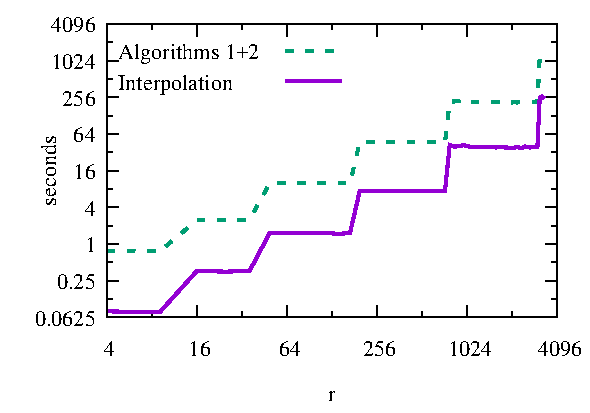
\includegraphics[width=0.49\textwidth]{explicit_isogenies/graphe-101.pdf}
\hfill
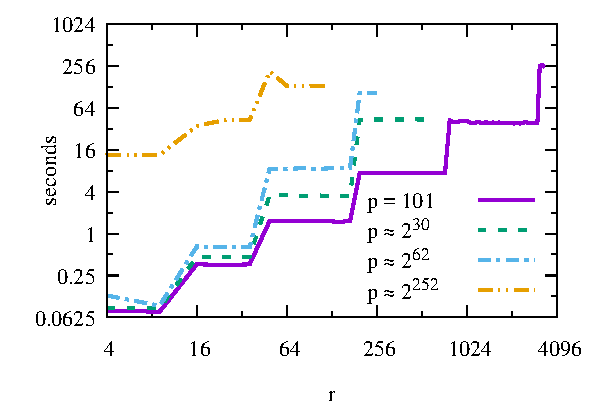
\includegraphics[width=0.49\textwidth]{explicit_isogenies/graphe-101-149-269.pdf}
\caption{Left: comparison of horizontal basis computation and
  interpolation phases, for a fixed curve defined over $\F_{101}$, and
  increasing $r$. Right: Comparison of one interpolation phase for
  $\F_{101}$, $\F_{2^{30}+669}$, $\F_{2^{62}+189}$ and $\F_{2^{252}+421}$, and increasing
  $r$. Plots in logarithmic scale.}
\label{expi:fig:benchs}
\end{figure}

We ran benchmarks on an Intel Xeon E5530 CPU clocked at 2.4GHz. We
fixed a base field $\F_q$ and an elliptic curve $E$ with height $h=3$ and $\beta=2$,
then ran our algorithm to compute the multiplication-by-$r$ isogeny
$E→E$, for $r$ increasing.  The torsion levels involved in the
computations varied from $2^3$ to $2^8$.  Figure~\ref{expi:fig:benchs}
(left) shows the running times for the computation of the horizontal
basis of $E[ℓ^k]$, and for one execution of the interpolation
step. Running times are close to linear in $r$,
as expected. The staircase behavior of our algorithm is apparent from
the plot. Since the interpolation steps must be repeated $\sim r$ times,
we focus on this step to compare the running
time for different base fields. In Figure~\ref{expi:fig:benchs} (right)
we observe that the dependency in $q$, although much better than in
Couveignes' original algorithm, is higher than what the theoretical 
analysis would predict. This may due to low-level implementation details
of SageMath, which, in the current implementation, are beyond our control.

In conclusion, our algorithm shows promise of being of practical
interest within selected parameter ranges. Generalizing it to work
with Atkin primes would considerably enlarge its applicability range;
we hope to develop such a generalization in a future work. On the
practical side, we plan to work on two improvements that seem within
reach. First, the reduction from generic curves to $ℓ$-maximal curves
seems superfluous and unduly expensive: it would be interesting to
generalize the concept of horizontal bases to any curve. Second, a
multi-modular approach interpolating on a torsion group of composite
order is certainly possible, and could improve the running time of our
algorithm by allowing it to work in smaller extension fields.


%\bibliographystyle{plain}
%\bibliography{refs}


%\appendix

\section{Galois classes in~$E[ℓ^k]$}
\label{expi:ap:galois}

We give here the full decomposition of $E[ℓ^k]$ in Galois classes.
This is a more precise form of Proposition~\ref{expi:prop:classes}~(v).
\begin{prop}\label{expi:prop:orbites-l-torsion}
Let~$E$ be an elliptic curve with $ℓ$-maximal endomorphism ring.
Assume $ℓ ≠ 2$, $λ ≡ μ ≡ 1 \pmod{ℓ}$ and let~$α = v_ℓ(λ-1), β=v_ℓ(μ-1)$.
Write~$ν(x, y) = \min (x+y, x+β-1, y+α-1)$
and~$ρ(x, y) = x+y - ν(x, y) = \max (0, x-α+1, y-β+1)$.
The decomposition of the group~$E[ℓ^k]$ in Galois classes is as follows:
\begin{enumerate}
\item for~$i, j = 1, …, k-1$:
$(ℓ-1)^2 · ℓ^{ν(i,j)}$ classes of size~$ℓ^{ρ(i,j)}$;
\item for~$i = 1, …, k-1$:
$(ℓ-1) · ℓ^{\min (i, α-1)}$ classes of size~$ℓ^{\max (0, i-α+1)}$, and
$(ℓ-1) · ℓ^{\min (i, β-1)}$ classes of size~$ℓ^{\max (0, i-β+1)}$;
\item the $ℓ^2$ singleton classes of~$E[ℓ]$.
% \item \todo{le cas où $ℓ=2$}
\end{enumerate}
\end{prop}
\begin{proof}
Fix a basis~$(P, Q)$ of~$E[ℓ^k]$ such that~$π(P)=λP$, $π(Q)=μQ$.
Studying the Galois orbits of~$E[ℓ^k]$
means studying the map~$ℤ_ℓ^2 → ℤ_ℓ^2, (x, y) ↦ (λ x, μ y)$.
In other words, the orbits correspond to elements of~$ℤ_ℓ^2$
modulo the \emph{multiplicative} subgroup generated by~$(λ, μ)$.
An easy way to describe this
is to consider a \emph{multiplicative lattice} in~$(ℚ_ℓ^×)^2$.

Let~$ξ$ be a primitive $(ℓ-1)$-th root of unity in~$ℤ_ℓ$.
Then by~\cite[Théorème II.3.2]{Serre.Arith},
the map~$f(x, y, z) = ℓ^x· ξ^y· \exp (ℓ z)$
is a group isomorphism between~$ℤ × (ℤ/(ℓ-1) ℤ) × ℤ_ℓ$ and~$ℚ_ℓ^{×}$.
For~$i ∈ \bcro{0,k-1}$ and~$c ∈ ℤ/(ℓ-1)ℤ$,
let~$V(i,c)$ be the image in $ℤ/ℓ^k ℤ$ of the map~$f(k-1-i,c,–)$:
then the multiplicative structure of $V(i, c)$
is that of a principal homogeneous space under~$ℤ/ℓ^i ℤ$.
We also define~$W(i,j,c,d) = V(i, c) · P \,+\, V(j, d) · Q ⊂ E[ℓ^k]$.

Since~$λ ≡ 1 \pmod{ℓ}$, we may write~$λ = f(0,0,u\, ℓ^{α-1})$
and~$μ = f(0,0, v\, ℓ^{β-1})$
for some~$u, v ∈ ℤ_ℓ^{×}$.
This implies that the set~$W(i,j,c,d)$ is stable under Galois.
Moreover, the orbits of~$W(i,j,c,d)$ correspond bijectively to
points of a fundamental domain of the lattice~$Λ_{i,j}$ generated by
the columns of~$\smat{ℓ^i & 0 & u ℓ^{α-1}\\ 0 & ℓ^j & v ℓ^{β-1}}$,
whereas the size of each orbit is~$[(ℤ/ℓ^i ℤ)×(ℤ/ℓ^j ℤ)\::\: Λ_{i,j}]$.
By using elementary column manipulations,
we find that the covolume of~$Λ_{i,j}$ is~$ℓ^{ν(i,j)}$,
hence the point~(i) of the proposition.
(The case~$i = j = 0$ yields singleton classes in~$E[ℓ]$).

The union of all the sets~$W(j,i,c,d)$
is exactly the set of all~$x P + y Q$ for~$x, y ≠ 0$.
We obtain the classes of~(ii) by considering
the sets~$V(i, c) · P$ and~$V(j,d) · Q$.
\end{proof}

We now state the equivalent proposition when~$ℓ = 2$.
The proof is much the same as in the odd case.

\begin{prop}\label{expi:prop:orbites-2-torsion}
Let~$E$ be an elliptic curve with $2$-maximal endomorphism ring.
Assume $λ ≡ μ ≡ 1 \pmod{4}$ and let~$α = v_2(λ-1), β=v_2(μ-1)$.
Write~$ν_2(x, y) = \min (x+y, x+β-2, y+α-2)$
and~$ρ_2(x, y) = x+y - ν_2(x, y) = \max (0, x-α+2, y-β+2)$.
The decomposition of the group~$E[2^k]$ in Galois classes is as follows:
\begin{enumerate}
\item for~$i, j = 1, …, k-2$:
$4 · 2^{ν_2(i,j)}$ classes of size~$2^{ρ_2(i,j)}$;
\item for~$i = 1, …, k-2$:
$4 · 2^{\min (i, α-2)}$ classes of size~$2^{\max (0, i-α+2)}$, and
$4 · 2^{\min (i, β-2)}$ classes of size~$2^{\max (0, i-β+2)}$.
\item the 16 singleton classes of~$E[4]$.
\end{enumerate}
\end{prop}
Note that if $λ$ or~$μ ≡ -1 \pmod{4}$ then
by replacing the base field by a quadratic extension,
we can always ensure that the condition $λ ≡ μ ≡ 1 \pmod{4}$ is
satisfied.
% \begin{proof}%<<<
% The proof is much the same as that of Prop.~\ref{expi:prop:orbites-l-torsion}.
% The case~$ℓ = 2$ of~\cite[Théorème II.3.2]{Serre.Arith}
% states that $f(x,y,z) = 2^x · (-1)^y · \exp (4z)$
% is an isomorphism between~$ℤ × (ℤ/2ℤ) × ℤ_2$ and~$ℚ_2^×$.
% Let~$V(i, c)$ be the image modulo~$2^k$ of~$f(k-2-i, c, -)$;
% then $V(i, c)$ has cardinal~$2^{i}$ for~$i ≥ 0$,
% while~$V(-1, 0) = V(-1, 1)$ is the singleton $\acco{2^{k-1}}$.
% 
% Let~$P, Q$ be diagonal generators of~$E[2^{k}]$
% and define~$W(i,j,c,d) = V(i,c) P + V(j,d) Q$;
% also write~$λ = f(0,0,2^{α-2} u)$, $μ = f(0,0,2^{β-2} v)$.
% Then the Galois orbits in~$W(i,j,c,d)$ correspond to $ℤ_2^2$ modulo
% the lattice~$Λ_{i,j} = \smat{2^{i}&0&2^{α-2} u\\0&2^{j}&2^{β-2} v}$.
% We find that $Λ_{i,j}$ has covolume~$2^{ν_2(i,j)}$.
% This gives the orbits of point~(i) of the proposition,
% while the case~$i = j = 0$ gives singleton orbits.
% 
% By considering the orbits of~$V(i,c) P + ε Q$ and~$ε P + V(i,c) Q$
% for~$ε ∈ \acco{0, 2^{k-1}}$, we obtain the orbits
% of point~(ii).
% \end{proof}%>>>
% >>>1

%  LocalWords:  isogeny morphisms Isogenies isogenies isogenous
%  LocalWords:  cardinality bijection Couveignes automorphism

% vim: ts=2:
%  LocalWords:  Frobenius endomorphism precomputation morphism
%  LocalWords:  subproduct factorizations asymptotical
}
{\def\C {\ensuremath{\mathsf{C}}}
\def\M {\ensuremath{\mathsf{M}}}
\def\Q {\ensuremath{\mathbb{Q}}}
\def\N {\ensuremath{\mathbb{N}}}
\def\R {\ensuremath{\mathbb{R}}}
\def\Z {\ensuremath{\mathbb{Z}}}
\def\F {\ensuremath{\mathbb{F}}}
\def\H {\ensuremath{\mathbb{H}}}
\def\K {\ensuremath{\mathbb{K}}}
\def\Kbar {\ensuremath{\overline{\mathbb{K}}}}
\def\L {\ensuremath{\mathbb{L}}}
\def\A {\ensuremath{\mathbb{A}}}
\def\B {\ensuremath{\mathbb{B}}}

\def\va {\ensuremath{\mathsf{a}}}
\def\vy {\ensuremath{\mathsf{y}}}
\def\vu {\ensuremath{\mathsf{u}}}
\def\vb {\ensuremath{\mathsf{b}}}
\def\vc {\ensuremath{\mathsf{c}}}

\def\mul {\ensuremath{\mathsf{mul}}}
\def\rem {\ensuremath{\mathsf{rem}}}
\def\cat {\ensuremath{\mathsf{cat}}}
\def\coeff {\ensuremath{\mathsf{coefficient}}}
\def\mulmod {\ensuremath{\mathsf{mulmod}}}
\def\rev {\ensuremath{\mathsf{rev}}}
\def\x {\ensuremath{\mathbf{x}}}
\def\Tr {\ensuremath{\mathrm{Tr}}}
\DeclareBoldMathCommand{\bxi}{\xi}
\DeclareBoldMathCommand{\bupsilon}{\upsilon}
\DeclareBoldMathCommand{\bzeta}{\zeta}
\DeclareBoldMathCommand{\blambda}{\lambda}

\newcounter{algo}
\renewcommand{\thealgo}{\thechapter.\arabic{algo}}

\newenvironment{algorithm_noendline}[4]{\begin{center}\begin{minipage}{0.98\textwidth}
      \refstepcounter{algo}
      \label{ff_compositum:#4}
      \rule{\textwidth}{0.2pt}\\
      \makebox[\textwidth][l]{\textbf{Algorithm~\thealgo}~\textsf{#1}}\\
      \rule[0.5\baselineskip]{\textwidth}{0.2pt}\\

      \vspace{-12pt}

      \parbox{\textwidth}{\textbf{Input} #2}
      \parbox{\textwidth}{\textbf{Output} #3}

      \vspace{-7pt}

      \begin{enumerate*}}{\end{enumerate*}
      \vspace{-11pt}
\end{minipage}\end{center}
}

\newenvironment{algorithm_endline}[4]{\begin{center}\begin{minipage}{0.98\textwidth}
      \refstepcounter{algo}
      \label{ff_compositum:#4}
      \rule{\textwidth}{0.2pt}\\
      \makebox[\textwidth][l]{\textbf{Algorithm~\thealgo}~\textsf{#1}}\\
      \rule[0.5\baselineskip]{\textwidth}{0.2pt}\\

      \vspace{-12pt}

      \parbox{\textwidth}{\textbf{Input} #2}
      \parbox{\textwidth}{\textbf{Output} #3}

      \vspace{-7pt}

      \begin{enumerate*}}{\end{enumerate*}
      \vspace{-11pt}
      \rule{\textwidth}{0.2pt}
\end{minipage}\end{center}
%\vspace{-0.5cm}
}

\floatstyle{plain}
\newfloat{algofloat}{thp}{bla}
\floatname{algofloat}{}

\newcommand{\ang}[1]{\langle#1\rangle}

\let\Def\definition
\let\endDef\enddefinition
\let\Theo\theorem
\let\endTheo\endtheorem
\let\Prop\proposition
\let\endProp\endproposition
\let\Lemma\lemma
\let\endLemma\endlemma

\chapter{Fast arithmetic for the algebraic closure of finite fields}

\begin{abstract}
  We present algorithms to construct and do arithmetic operations in
  the algebraic closure of the finite field $\mathbb{F}_p$. Our
  approach is inspired by algorithms for constructing irreducible
  polynomials, which first reduce to prime power degrees, then use
  composita techniques. We use similar ideas to give efficient
  algorithms for embeddings and isomorphisms.
\end{abstract}

{\small This article was authored with Javad Doliskani and Éric
  Schost. It originally appeared in the \textit{Proceedings of the
    38th International Symposium on Symbolic and Algebraic
    Computation} (ISSAC 2013), \doi{10.1145/2465506.2465956}.}

%%%%%%%%%%%%%%%%%%%%%%%%%%%%%%%%%%%%%%%%%%%%%%%%%%%%%%%%%%%%
%%%%%%%%%%%%%%%%%%%%%%%%%%%%%%%%%%%%%%%%%%%%%%%%%%%%%%%%%%%%
%%%%%%%%%%%%%%%%%%%%%%%%%%%%%%%%%%%%%%%%%%%%%%%%%%%%%%%%%%%%

\section{Introduction}

Several computer algebra systems or libraries, such as
Magma~\cite{MAGMA}, Sage~\cite{Sage}, NTL~\cite{shoup2003ntl},
PARI~\cite{Pari} or Flint~\cite{Hart2010}, offer built-in
features to build and compute in arbitrary finite fields. At the core
of these designs, one finds algorithms for building irreducible
polynomials and algorithms to compute embeddings and isomorphisms.
The system used in Magma (one of the most complete we know of) is
described in~\cite{bosma+cannon+steel97}.

Previous algorithms typically rely on linear algebra techniques, for
instance to describe embeddings or isomorphisms (this is the case for
the algorithms in~\cite{bosma+cannon+steel97}, but also for those
in~\cite{LenstraJr91,Allombert02}). Unfortunately, linear algebra
techniques have cost at least quadratic in the degree of the
extensions we consider, and (usually) quadratic memory requirements.
Our goal here is to replace linear algebra by polynomial arithmetic,
exploiting fast polynomial multiplication to obtain algorithms of
quasi-linear complexity. As we will see, we meet this goal for
several, but not all, operations.

\noindent{{\bf \rm Setup.}}
Let $p$ be a prime (that will be fixed throughout this paper). We are
interested in describing extensions $\F_{p^n}$ of $\F_p$; such an
extension has dimension $n$ over $\F_p$, so representing an element in
it involves $n$ base field elements.

It is customary to use polynomial arithmetic to describe these
extensions (but not necessary: Lenstra's algorithm~\cite{LenstraJr91}
uses a multiplication tensor). For an extension degree $n$, a
first step is to construct an irreducible polynomial $Q_n$ of degree
$n$ in $\F_p[x]$. Identifying $\F_{p^n}$ with $\F_p[x]/\ang{Q_n}$,
operations $(+,\times,\div)$ in $\F_p[x]/\ang{Q_n}$ all take
quasi-linear time in~$n$.

However, this is not sufficient: we also want mechanisms for
e.g. field embeddings. Given irreducible polynomials $Q_m$ and $Q_n$
over $\F_p$, with $\deg(Q_m)=m$ dividing $\deg(Q_n)=n$, there exist
algorithms to embed $\F_p[x]/\ang{Q_m}$ in 
$\F_p[x]/\ang{Q_n}$ (for the system to be consistent, these embeddings
must be {\em compatible}~\cite{bosma+cannon+steel97}). However, most
algorithms use linear algebra techniques.

To bypass these issues, we use an approach inspired by Shoup's
algorithm for computing irreducible polynomials~\cite{Shoup_1990,shoup94}
(see also~\cite{couveignes+lercier11,lenstra+desmit08-stdmodels}):
first reduce to the case of prime power degrees, then use composita
techniques, in a manner that ensures compatibility of the embeddings
automatically.

\smallskip\noindent{{\bf \rm Background: towers.}}
Suppose that for any prime $\ell$, an {\em $\ell$-adic tower} over
$\F_p$ is available. By this, we mean a family of polynomials
$(T_{\ell,i})_{i \ge 1}$, with $T_{\ell,i} \in \F_p[x_1,\dots,x_i]$,
monic of degree $\ell$ in $x_i$, such that for all $i$ the ideal
$\ang{T_{\ell,1},\dots,T_{\ell,i}}$ is maximal in $\F_p[x_1,\dots,x_i]$.
Our model of the field with $p^{\ell^i}$ elements could then
be
$\K_{\ell^i}=\F_p[x_1,\dots,x_i]/\ang{T_{\ell,1},\dots,T_{\ell,i}}$,
but we prefer to work with univariate polynomials (the cost of
arithmetic operations is higher in the multivariate basis).  

For $1 \le i \le n$, let then $Q_{\ell,i}$ be the minimal polynomial
of $x_i$ in the extension $\K_{\ell^n}/\F_p$. This polynomial does
not depend on $n$, but only on $i$; it is monic, irreducible of degree
$\ell^i$ in $\F_p[x_i]$ and allows us to define $\F_{p^{\ell^i}}$ as
$\F_p[x_i]/\ang{Q_{\ell,i}}$.
For $1 \le i \le j \le n$, let further $Q_{\ell,i,j-i}$ be the minimal
polynomial of $x_j$ in the extension $\F_p[x_i]/\ang{Q_{\ell,i}} \hookrightarrow
\K_{\ell^n}$ (as above, it does not depend on $n$). This polynomial is
monic, irreducible of degree $\ell^{j-i}$ in
$\F_{p^{\ell^i}}[x_j]=\F_p[x_i]/\ang{Q_{\ell,i}}[x_j]$.

Thus, $\F_p[x_j]/\ang{Q_{\ell,j}}$ and
$\F_p[x_i,x_j]/\ang{Q_{\ell,i},Q_{\ell,i,j-i}}$ are two models for
$\F_{p^{\ell^j}}$. Provided conversion algorithms between these
representations are available, we can perform embeddings (that will
necessarily be compatible) between different levels of the $\ell$-adic
tower, i.e.\ extensions of degrees $(\ell^i)_{i \ge 1}$.

Such towers, together with efficient conversion algorithms, were
constructed in the cases $\ell = p$
in~\cite{cantor89,couveignes00,df+schost12}, $\ell=2$
in~\cite{DoSc12}, and for other values of $\ell$ in~\cite{DeDoSc13}.
Thus, it remains to give algorithms to ``glue'' towers defined for
different values of $\ell$. This is the purpose of this paper.

\smallskip\noindent{{\bf \rm Our contribution.}} The algorithms used
to construct towers are inspired by those used
in~\cite{Shoup_1990,shoup94,couveignes+lercier11} to build irreducible
polynomials. Also used in these references is the following idea: let
$Q_m(x)$ and $Q_n(y)$ be irreducible polynomials over $\F_p$, with
coprime degrees $m,n>1$, and having respectively $(a_i)_{1 \le i
  \le m}$ and $(b_j)_{1 \le j \le n}$ as roots in an algebraic closure
of $\F_p$. Then their {\em composed product} $Q_{mn} = \prod_{1 \le i
  \le m, 1 \le j \le n} (z- a_i b_j)$ is irreducible of degree $mn$ in
$\F_p[z]$.

In this paper, we use an {\em algebraic complexity model}, where the
cost of an algorithm is counted in terms of the number of operations
$(+,\times,\div)$ in $\F_p$.  If the goal is building irreducible
polynomials, then computing $Q_{mn}$ is enough: an algorithm given
in~\cite{BoFlSaSc06} has quasi-linear cost in $mn$. Our goal here is
to give algorithms for further operations: computing embeddings of the
form $\varphi_x: \F_p[x]/\ang{Q_m}\to \F_p[z]/\ang{Q_{mn}}$ or
$\varphi_y: \F_p[y]/\ang{Q_n}\to \F_p[z]/\ang{Q_{mn}}$, and the
isomorphism $\Phi: \F_p[x,y]/\ang{Q_m,Q_n}\to \F_p[z]/\ang{Q_{mn}}$ or
its inverse.

Standard solutions to these questions exist, using {\em modular
  composition} techniques: once the image $S=\Phi(x)$ is known,
computing $\varphi_x(a)$ amounts to computing $a(S) \bmod Q_{mn}$;
similarly, computing $\Phi(b)$, for $b$ in $\F_p[x,y]/\ang{Q_m,Q_n}$,
amounts to computing $b(S,T) \bmod Q_{mn}$, with $T=\Phi(y)$.  This
can be done using the Brent and Kung algorithm~\cite{brent+kung}: the
resulting cost is $O(m n^{(\omega+1)/2}) \subset O(m n^{1.69})$ for
$\varphi_x$ (see the analysis in~\cite{shoup94}) and $O((m
n)^{(\omega+1)/2}) \subset O(m^{1.69} n^{1.69})$ for $\Phi$ or its
inverse~\cite{PoSc13b}. Here, we denote by $\omega$ a constant in
$(2,3]$ such that one can multiply matrices of size $m$ over any ring
  $A$ using $O(m^\omega)$ operations $(+,\times)$ in~$A$; using the
  algorithms of~\cite{coppersmith+winograd,Williams12}, we can take
  $\omega \le 2.38$.

Our main result improves on these former ones. We denote by $\M:\N \to
\N$ a function such that for any ring $A$, polynomials in $A[x]$ of
degree at most $n$ can be multiplied in $\M(n)$ operations
$(+,\times)$ in $A$, and we make the usual super-linearity assumptions
on $\M$~\cite[Chapter~8]{vzGG}.
\begin{Theo}\label{ff_compositum:theo:main}
  One can apply $\varphi_x$ (resp.\ $\varphi_y$) to an element of
  $\F_p[x]/\ang{Q_m}$ (resp.\ $\F_p[x]/\ang{Q_n}$), or invert it on its
  image, using $O(n\M(m)+m\M(n))$ operations in $\F_p$.

  Suppose that $m \le n$. Then one can
  apply $\Phi$ to an element of $\F_p[x,y]/\ang{Q_m, Q_n}$ or invert
  it using either $O(m^2 \M(n))$ or $O(\M(mn)n^{1/2}+\M(m)
  n^{(\omega+1)/2} )$ operations in $\F_p$.
\end{Theo}

Using the $O\tilde{~}$ notation to neglect polylogarithmic factors, we
can take $\M(n) \in O\tilde{~}(n)$.  Our algorithm for embeddings and
their inverses has quasi-linear cost $O\tilde{~}(mn)$.  Those for
$\Phi$ or $\Phi^{-1}$ have respective costs $O\tilde{~}(m^2 n)$ and
$O\tilde{~}(m n^{(\omega+1)/2})$; the minimum of the two is in
$O\tilde{~}( (mn)^{2\omega/(\omega+1)})$; for $\omega \in (2,3]$, the
  resulting exponent is in $(1.333\dots, 1.5]$.  

If $S=\Phi(x)$ and $T=\Phi(y)$ are known, a result by Kedlaya and
Umans~\cite{KeUm11} for modular composition, and its extension
in~\cite{PoSc13a}, yield an algorithm with {\em bit complexity}
essentially linear in $mn$ and $\log(p)$ on a RAM. Unfortunately,
making these algorithms competitive in practice is challenging; we are
not aware of any implementation of them. It is also worth noting that
our algorithms apply in a more general setting than finite fields
(mild assumptions are required).

\smallskip\noindent{\bf Outline.}  Section~\ref{ff_compositum:sec:prelim} presents
basic algorithms for polynomials and their transposes.
Section~\ref{ff_compositum:sec:trace} introduces the main idea behind our
algorithms: the trace induces a duality on algebras of the form
$\F_p[x]/\ang{Q}$, and some conversion algorithms are straightforward
in dual bases; the algorithms are detailed in
Section~\ref{ff_compositum:sec:emb-iso}. Section~\ref{ff_compositum:sec:fpbar} explains how the
results in this paper can be used in order to construct the algebraic
closure of $\F_p$. We conclude with experimental results.

%%%%%%%%%%%%%%%%%%%%%%%%%%%%%%%%%%%%%%%%%%%%%%%%%%%%%%%%%%%%
%%%%%%%%%%%%%%%%%%%%%%%%%%%%%%%%%%%%%%%%%%%%%%%%%%%%%%%%%%%%
%%%%%%%%%%%%%%%%%%%%%%%%%%%%%%%%%%%%%%%%%%%%%%%%%%%%%%%%%%%%

\section{Preliminaries}\label{ff_compositum:sec:prelim}

We recall first previous results concerning polynomial arithmetic and
transposition of algorithms. In all this section, a ground field $k$,
not necessarily finite, is fixed. For integers $m,n$, we denote by
$k[x]_m$ (resp.\ $k[x,y]_{m,n}$) the set of polynomials $P$ in $k[x]$
with $\deg(P) <m$ (resp.\ $P$ in $k[x,y]$ with $\deg(P,x) <m$ and
$\deg(P,y)<n$).

%%%%%%%%%%%%%%%%%%%%%%%%%%%%%%%%%%%%%%%%%%%%%%%%%%%%%%%%%%%%

\subsection{Polynomial multiplication and remainder}

We start with some classical algorithms and their complexity. For all
the algorithms that follow, all polynomials are written on the
canonical monomial basis (this is innocuous for the moment, but other
bases will be discussed below).

The product of two polynomials of respective degrees at most $m$ and
$n$ can be computed in $\M(\max(m,n))$ operations in $k$.  If $P$ is a
monic polynomial of degree $m$ in $k[x]$, for $n \ge 1$, we let
$\rem(.,P,n)$ be the operator
$$
\begin{array}{cccc}
\rem(.,P,n): &k[x]_n& \to &k[x]_{m}\\
& a & \mapsto & a \bmod P.
\end{array}$$ 
For $n \le m$, this is free of cost. For $n > m$, this can be computed
in time $O(n\M(m)/m)$ using the Cook-Sieveking-Kung algorithm and
blocking techniques~\cite[Ch.~5.1.3]{Bostan10}. Defining
$A=k[x]/\ang{P}$, and choosing a fixed $b \in A$, we can then define
the mapping $\mulmod(.,b,P)$, which maps $a \in A$ to $ab \bmod P$; it
can be computed in time $O(\M(m))$. Finally, given an integer $m$, the
reversal operator in length $m$ is 
$$
\begin{array}{cccc} \rev(.,m): &k[x]_m &\to& k[x]_m \\ & a & \mapsto &
x^{m-1} a(1/x).
\end{array}$$ 

%%%%%%%%%%%%%%%%%%%%%%%%%%%%%%%%%%%%%%%%%%%%%%%%%%%%%%%%%%%%

\subsection{Duality and the transposition principle}\label{ff_compositum:ssec:duality}

The {\em transposition principle} is an algorithmic result which
states that, given an algorithm that performs a matrix-vector product
$u \mapsto M u$, one can deduce an algorithm with essentially the same
cost which performs the transposed matrix-vector product $v \mapsto
M^t v$~\cite[Ch.~13]{burgisser+clausen-shokrollahi}.

Following~\cite{df+thesis}, we give here a more abstract presentation
of the transposition principle, using the algebraic theory of duality
(see~\cite[Ch.~IX.1.8]{BourbakiAlgCom9}). The added level of abstraction
will pay off by greatly simplifying the proofs of the next sections.

Let $E$ and $F$ be $k$-vector spaces, with $\dim(E)=\dim(F)<\infty$,
and suppose that $\ang{.,.}: E\times F \to k$ is a non-degenerate
bilinear form.  Then, to any vector space basis $\bxi=(\xi_i)_i$ of
$E$, we can associate a unique \emph{dual basis}
$\bxi^\ast=(\xi_i^\ast)_i$ of $F$ such that $ \ang{\xi_i,\xi^\ast_j} =
\delta_{i,j}$ (the Kronecker symbol).  In other words, given $a$ in
$F$, the coefficients $(a_i)$ of $a$ on the basis $\bxi^\ast$ are
given by $a_i=\ang{\xi_i, a}$.

For example, denote by $E^\ast$ the dual space of $E$, i.e.\ the
$k$-linear forms on $E$. The bilinear form on $E\times E^\ast$ defined
by with $\ang{v,\ell}=\ell(v)$ for all $v\in E$ and $\ell \in E^*$ is
non-degenerate. This is indeed the canonical example, and any
non-degenerate form, is isomorphic to this one. We will see in the
next section another family of examples, with $E=F$.

Let $E',F'$ be two further vector spaces, with $\dim(E')=\dim(F')<\infty$ and
let $\ang{.,.}'$ be a bilinear form $E'\times F' \to k$. Then, to
any linear mapping $u:E\to E'$, one associates its {\em dual}
(with respect to $\ang{.,.}$ and $\ang{.,.}'$), which is a linear
mapping $u^t: F' \to F$ characterized by the equality
$\ang{u(a),b'}'=\ang{a,u^t(b')}$, for all $a\in E$ and $b'\in F'$.

Let as above $\bxi$ be a basis of $E$, and let $\bxi^\ast$ be
the dual basis of $F$; consider as well a basis $\bupsilon$ of $E'$ and
its dual basis $\bupsilon^\ast$ of $F'$. If $M$ is the matrix of $u$ in
the bases $(\bxi,\bupsilon)$, the matrix of $u^t$ in the bases
$(\bupsilon^\ast,\bxi^\ast)$ is the transpose of $M$. 

As presented in~\cite{bostan+lecerf+schost:tellegen,df+thesis}, the
transposition principle is an algorithmic technique that, given an
algorithm to compute $u: E \to E'$ in the bases $(\bxi,\bupsilon)$,
yields an algorithm for the dual map $u^t: F' \to F$ in the bases
$(\bupsilon^\ast,\bxi^\ast)$. The two algorithms have same cost, up to
$O(\dim(E)+\dim(E'))$. In a nutshell, starting from an algorithm relying
on a few basic operations (such as polynomial or matrix
multiplication), its transpose is obtained by transposing each basic
subroutine, then reversing their order.

Let us briefly review the transposes of operations described in the
previous subsection. The transpose of polynomial multiplication is
described in~\cite{bostan+lecerf+schost:tellegen}; it is closely
related to the {\em middle product}~\cite{hanrot+quercia+zimmermann}.
Let next $P$ be monic of degree $m$, and define $A=k[x]/\ang{P}$. As
shown in~\cite{bostan+lecerf+schost:tellegen}, the dual map of \rem
$$
\begin{array}{cccc}
\rem^t(.,P,n): &A^\ast& \to &k[x]_n^\ast
\end{array}$$ 
is equivalent to \emph{linear sequence extension}:
it takes as input the initial $m$ values of a linear recurring
sequence of minimal polynomial $P$, and outputs its first $n$ values.
% LFSRs give a simple, though suboptimal, implementation of this
% operator.
The transposed version of the Cook-Sieveking-Kung fast Euclidean
division algorithm yields an algorithm with cost $O(n\M(m)/m)$
operations in $k$~\cite{vzgathen+shoup92:journal,shoup99}.

For a fixed $b\in A$, the transpose of \mulmod\ is the map
$$
\begin{array}{cccc}
\mulmod^t(.,b,P): & A^\ast &\to& A^\ast \\
& \ell & \mapsto & b\cdot\ell,
\end{array}
$$ 
where $b \cdot \ell$ is defined by $(b \cdot \ell)(a)
=\ell(ab)$. Algorithms for $\mulmod^t$ have been subject to much
research (for instance, Berlekamp's \emph{bit serial
  multiplication}~\cite{Berlekamp82} is a popular arithmetic circuit
for $\mulmod^t$ in the case $k=\F_2$); algorithms of cost $O(\M(m))$
are given in~\cite{shoup99,bostan+lecerf+schost:tellegen}.

Lastly, the reversal operator on $k[x]_m$ is its own transpose.

%%%%%%%%%%%%%%%%%%%%%%%%%%%%%%%%%%%%%%%%%%%%%%%%%%%%%%%%%%%%
%%%%%%%%%%%%%%%%%%%%%%%%%%%%%%%%%%%%%%%%%%%%%%%%%%%%%%%%%%%%
%%%%%%%%%%%%%%%%%%%%%%%%%%%%%%%%%%%%%%%%%%%%%%%%%%%%%%%%%%%%

\section{Trace and duality}\label{ff_compositum:sec:trace}\label{ff_compositum:ssec:conversions}\label{ff_compositum:sec:trace-formulas}

Next, we discuss some classical facts about the trace form, and give
algorithms to change between monomial bases and their duals. In all
this section, $k$ is a perfect field. General references for the
following are~\cite{Kunz86,Cox-Little-OShea:UAG2005}.

\smallskip\noindent{{\bf \rm Traces in reduced algebras.}} 
Let $s$ be a positive integer and $I$ a zero dimensional radical ideal
in $k[x_1,\dots,x_s]$. Thus, $A=k[x_1,\dots,x_s]/I$ is a reduced
$k$-algebra of finite dimension $d$, where $d$ is the cardinality of
$V=V(I) \subset\overline{k}^s$ (in general, $A$ is not a field).

Let $a$ be in $A$. As we did in the case of one variable, we associate
to $a$ the endomorphism of multiplication-by-$a$ $M_a: A \to A$ given
by $M_a(b)=ab$.  Even though $A$ may not be a field, we still define
the {\em minimal polynomial} of $a$ as the minimal polynomial of
$M_a$; since $I$ is radical, this polynomial is squarefree, with roots
$a(x)$, for $x$ in $V$. Similarly, the \emph{trace} of $a$
is the trace of $M_a$, and denote it by $\tau_I(a)$. Because $I$
is radical, the trace defines a non-degenerate bilinear form on
$A\times A$, given by $\ang{a,b}_I = \tau_I(ab)$.

Thus, to any basis $\bxi=(\xi_i)_{0 \le i < d}$ of $A$, one can
associate a dual basis $\bxi^\ast=(\xi^\ast_i)_{0 \le i < d}$,
such that $\ang{\xi_i, \xi^\ast_j}_I=\delta_{i,j}$ for all
$i,j$.  It will be useful to keep in mind that for $a \in A$, its
expression on the dual basis $\bxi^\ast$ is $a=\sum_{0 \le i < d}
\ang{a,\xi_i}_I \xi^\ast_i$.

We now describe algorithms for converting between the monomial basis and its
dual, in two particular cases, involving respectively univariate
and bivariate polynomials. In both cases, our conclusion will be that
such conversions have quasi-linear complexity.

\smallskip\noindent{{\bf \rm Univariate conversion.}} 
Let $P$ be monic of degree $m$ and squarefree in $k[x]$, and define
$A=k[x]/\ang{P}$. We denote by $P'$ its derivative and by $\tau_P$ the trace modulo the ideal $\ang{P}$.

The $k$-algebra $A$ is endowed with the canonical monomial basis
$\bxi=(x^i)_{0 \le i < m}$. In view of what was said in the previous
subsection, the coefficients of an element $a \in A$ on the dual basis
$\bxi^\ast$ are the traces $\tau_P(ax^i)_{0 \le i < m}$. The following
lemma shows that the generating series of these traces is rational,
with a known denominator; this will be the key to the conversion
algorithm. This is a restatement of well-known results, see for
instance the proof of~\cite[Theorem~3.1]{rouiller99}.

\begin{Lemma}\label{ff_compositum:lemma:trace:1}
  For $a$ in $A$, the following
  holds in $k[[x]]$:
  $$\sum_{i \ge 0} \tau_P(a x^i) x^i = \frac{\rev( P' a \bmod P,m)}{\rev(P,m+1)}.$$
\end{Lemma}

Some well-known algorithms to convert between $\bxi$ and $\bxi^\ast$
follow easily. In these algorithms, and all that follows, input and
output are vectors (written in {\sf sans serif} font).

\begin{algorithm_noendline}
{MonomialToDual$(\va,P)$}
{$\va=(a_i)_{0 \le i < m} \in k^m$, $P$ monic squarefree in $k[x]$ of degree $m$}
{$(\tau_P(a x^i))_{0 \le i < m}$, with $a=\sum_{0 \le i < m} a_i x^i$}
{algo:minpolytotrace}
\item $T = 1/\rev(P, m+1) \bmod x^m$
\item $b = \rev(P' \sum_{0 \le i < m} a_i x^i \bmod P, m)\, T \bmod x^m$
\item {\bf return} $(\coeff(b,x^i))_{0 \le i < m}$
\end{algorithm_noendline}

\begin{algorithm_endline}
{DualToMonomial$(\vb, P)$}
{$\vb=(b_i)_{0 \le i < m} \in k^m$, $P$ monic squarefree in $k[x]$ of degree $m$}
{$(a_i)_{0 \le i < m}$ such that $\tau_P(\sum_{0 \le i < m} a_i x^{i+j}) = b_j$ for all $j$}
{algo:tracetopoly}
\item $S = 1/P' \bmod P$
\item $b= \rev(P,m+1) \sum_{0 \le i < m} b_i x^i \bmod x^m$
\item $c= \rev(b, m)$
\item $d =c\, S \bmod P$
\item {\bf return} $(\coeff(d,x^i))_{0 \le i < m}$
\end{algorithm_endline}

\begin{Lemma}\label{ff_compositum:lemma:uniconv}
  Algorithms~\ref{ff_compositum:algo:minpolytotrace} and~\ref{ff_compositum:algo:tracetopoly} are
  correct. The former uses $O(\M(m))$ operations in $k$, the
  latter $O(\M(m)\log(m))$.  If the polynomial $S=1/P' \bmod P$ is
  known, the running time of Algorithm~\ref{ff_compositum:algo:tracetopoly} drops to
  $O(\M(m))$.
\end{Lemma}
\begin{proof}
  Correctness follows from Lemma~\ref{ff_compositum:lemma:trace:1}.  Once we point
  out that power series inversion modulo $x^m$ can be done in time
  $O(\M(m))$, the running time analysis of the former is
  straightforward. For Algorithm~\ref{ff_compositum:algo:tracetopoly}, the dominant
  part is the computation of $S$, which takes time $O(\M(m)\log(m))$
  by fast XGCD; all other steps take $O(\M(m))$ operations in $k$.
\end{proof}

\vspace{-1ex}\noindent{{\bf \rm Bivariate conversions.}} Now we consider two monic
squarefree polynomials $P$ in $k[x]$ of degree $m$, and $Q$ in $k[y]$
of degree $n$. We define $A=k[x,y]/I$, with $I=\ang{P,Q}$,
then $A$ has the canonical monomial basis $(x^i y^j)_{0 \le i <m, 0
  \le j <
  n}$. %% For $a$ in $k[x,y]$, $a \bmod I$ denotes the polynomial in
%% $k[x,y]_{m,n}$ obtained by reduction modulo both $P$ and $Q$.
We
denote by $\tau_I$ the trace modulo $I$, and by $\tau_P$ and $\tau_Q$
the traces modulo respectively $\ang{P}$ and $\ang{Q}$.

In addition to its monomial basis, $A$ can be endowed with a total of
four natural bases, which are described as follows. Let $\bxi=(x^i)_{0
  \le i < m}$ and $\bupsilon=(y^i)_{0 \le j < n}$ be the monomial
bases of respectively $k[x]/\ang{P}$ and $k[y]/\ang{Q}$; let
$\bxi^\ast$ and $\bupsilon^\ast$ be their respective dual bases, with
respect to $\tau_P$ and $\tau_Q$. The monomial basis seen above is
$\bxi \otimes \bupsilon$; the other combinations $\bxi^\ast \otimes
\bupsilon$, $\bxi \otimes \bupsilon^\ast$ and $\bxi^\ast \otimes
\bupsilon^\ast$ are bases of $A$ as well. After a precomputation of
cost $O(\M(m)\log(m) + \M(n)\log(n))$, Lemma~\ref{ff_compositum:lemma:uniconv} shows
that conversions between any pair of these bases can be done using
$O(n\M(m)+m\M(n))$ operations in $k$ (by applying the univariate
conversion algorithms $n$ times $x$-wise and / or $m$ times
$y$-wise). Using fast multiplication, this is quasi-linear in the
dimension $mn$ of $A$.

The following easy lemma will help us exhibit the duality
relationships between these bases; it follows from the fact that $A$
is the tensor product of $k[x]/\ang{P}$ and $k[y]/\ang{Q}$.

\begin{Lemma}
  \label{ff_compositum:lemma:traces:PQR1}
  Let $b$ be in $k[x]/\ang{P}$ and $c$ in $k[y]/\ang{Q}$. Then we have
  $\tau_I(bc) = \tau_P(b) \ \tau_Q(c)$.
\end{Lemma}
This lemma implies that $\bxi \otimes \bupsilon$ and $\bxi^\ast
\otimes \bupsilon^\ast$ are dual to one another with respect to
$\ang{.,.}_I$, as are $\bxi^\ast \otimes \bupsilon$ and $\bxi
\otimes \bupsilon^\ast$. 

%%%%%%%%%%%%%%%%%%%%%%%%%%%%%%%%%%%%%%%%%%%%%%%%%%%%%%%%%%%%
%%%%%%%%%%%%%%%%%%%%%%%%%%%%%%%%%%%%%%%%%%%%%%%%%%%%%%%%%%%%
%%%%%%%%%%%%%%%%%%%%%%%%%%%%%%%%%%%%%%%%%%%%%%%%%%%%%%%%%%%%

\section{Embedding and isomorphism} \label{ff_compositum:sec:emb-iso}

This section contains the main algorithms of this paper. We consider
two squarefree polynomials $P(x)$ and $Q(y)$ of respective degrees $m$
and $n$, with coefficients in a perfect field $k$. Let us then set
$A=k[x,y]/I$, where $I$ is the ideal $\ang{P(x),Q(y)}$ in $k[x,y]$. In
all this section, {\em we assume that $xy$ is a generator of $A$ as a
  $k$-algebra}. 

The main example we have in mind is the following: $k$ is a finite
field and both $P$ and $Q$ are irreducible, with $\gcd(m,n)=1$. Then
our assumption is satisfied and in addition $A$ is a field, namely,
the {\em compositum} of the fields $k[x]/\ang{P}$ and $k[y]/\ang{Q}$,
see~\cite{BrCa87}. More generally, if we let $(r_i)_{i<m}$ be the
roots of $P$ in an algebraic closure of $k$, and let $(s_j)_{j<n}$ be
the roots of $Q$, then as soon as the products $r_i s_j$ are pairwise
distinct, $xy$ generates $A$ as a $k$-algebra.

Let $R \in k[z]$ be the minimal polynomial of $xy$ in the extension
$A/k$ (equivalently, the roots of $R$ are the products $r_i s_j$);
this polynomial is known as the {\em composed product} of $P$ and $Q$,
and we will denote it $R = P \odot Q$. As $k$-algebras, we have $A
\simeq k[x]/\ang{R}$, so there exist embeddings $\varphi_x$, $\varphi_y$, 
and an isomorphism $\Phi$
of the form
$$
\begin{array}{ccccc}
&\varphi_x: & k[x]/\ang{P} & \to & k[z]/\ang{R}\\[2mm]
& \varphi_y: & k[y]/\langle Q \rangle & \to & k[z]/\ang{R}\\[2mm]
\text{and}& \Phi:&  A=k[x,y]/\langle P,Q\rangle & \to & k[z]/\ang{R} \\
& &  xy & \mapsfrom & z.
\end{array}$$
In this section, we give algorithms for computing $R$, applying
$\varphi_x$, $\varphi_y$ and their sections, and finally $\Phi$ and its inverse. Except from the
computation of $R$, these are all linear algebra problems. If $R$ and
the images $S=\Phi(x),T=\Phi(y)$ are known, then as was explained in
the introduction, direct solutions are available for both $\varphi_x$
(or $\varphi_y$) and $\Phi$ -- modular composition -- but none of
these approaches have a quasi-linear running time.

We take a different path. Our algorithms have quasi-linear running
time for $\varphi_x$ and $\varphi_y$ and improve on the Brent-Kung
algorithm for $\Phi$. Put together, Lemmas~\ref{ff_compositum:lemma:algo:embed}
to~\ref{ff_compositum:lemma:tiso2} below prove Theorem~\ref{ff_compositum:theo:main}. One of the
key aspects of these algorithms is that some are written in the usual
monomial bases, whereas others are naturally expressed in the
corresponding dual bases. From the complexity point of view, this is
not an issue, since we saw that all change-of-bases can be done in
quasi-linear time.

In what follows, we write $\tau_P,\tau_Q,\tau_R,\tau_I$ for the traces
modulo the ideals $\ang{P}\subset k[x]$, $\ang{Q} \subset k[y]$,
$\ang{R} \subset k[z]$ and $I=\ang{P,Q} \subset k[x,y]$; the
corresponding bilinear forms are denoted by $\ang{.,.}_P$, \dots

We let $\bxi=(x^i)_{0 \le i < m}$, $\bupsilon=(y^i)_{0 \le j <
  n}$ and $\bzeta = (z^i)_{0 \le i < mn}$ be the monomial bases of
respectively $k[x]/\ang{P}$, $k[y]/\ang{Q}$ and $k[z]/\ang{R}$. We also let
$\bxi^\ast=(\xi^\ast_i)_{0 \le i <m}$,
$\bupsilon^\ast=(\upsilon^\ast_i)_{0 \le i < n}$ and
$\bzeta^\ast=(\zeta^\ast_i)_{0 \le i < mn}$ be the dual bases, with
respect to respectively $\ang{.,.}_P$, $\ang{.,.}_Q$ and
$\ang{.,.}_R$.

Finally, we denote by $\vu_P \in k^m$ the vector of the coordinates of
$1 \in k[x]/\ang{P}$ on the dual basis $\bxi^\ast$; the vector
$\vu_Q$ is defined similarly. These vectors can both be computed in
quasi-linear time, since we have, for instance, $\vu_P = {\sf
  MonomialToDual}((1,0,\dots,0), P)$. Thus, in what follows, we assume
that these vectors are known.

%%%%%%%%%%%%%%%%%%%%%%%%%%%%%%%%%%%%%%%%%%%%%%%%%%%%%%%%%%%%

\subsection{Embedding and computing $R$} 

We first show how to compute the embeddings $\varphi_x$ and
$\varphi_y$, and their inverses in quasi-linear time in $mn$. We
actually give a slightly more general algorithm, which computes the
restriction of $\Phi$ to the set $$\Pi= \{bc \,\mid\, b\in
k[x]/\ang{P},\ c\in k[y]/\ang{Q}\} \subset k[x,y]/\ang{P,Q}.$$ We
will use the following lemma, which results from the base independence
of the trace (the second equality is Lemma~\ref{ff_compositum:lemma:traces:PQR1}).

\begin{Lemma}
  \label{ff_compositum:lemma:traces:PQR}
  Let $b$ be in $k[x]/\ang{P}$ and $c$ in $k[y]/\ang{Q}$. Then we have
  $\tau_R(\Phi(bc)) = \tau_I(bc) = \tau_P(b) \ \tau_Q(c)$.
\end{Lemma}
An easy consequence is that $\tau_R(z^i) =
\tau_P(x^i)\tau_Q(y^i)$. From this lemma, we also immediately deduce
Algorithm~\ref{ff_compositum:algo:embed}, which computes the image in $k[z]/\ang{R}$
of any element of $\Pi$, with inputs and outputs written on dual
bases.

%\vspace{-2ex}

\begin{algorithm_endline}
{Embed$(\vb,\vc,r)$}
{$\vb=(b_i)_{0 \le i < m} \in k^m$, $\vc=(c_i)_{0 \le i < n} \in k^n$
    an optional integer $r \ge mn$ set to $r=mn$ by default}
{$\va=(a_i)_{0 \le i < r} \in k^{r}$}
{algo:embed}
\item $(t_i)_{0\le i<r} = \rem^t(\vb,P,r)$
\item $(u_i)_{0\le i<r} = \rem^t(\vc,Q,r)$
\item {\bf return}$(t_i u_i)_{0 \le i <r}$
\end{algorithm_endline}

\begin{Lemma}\label{ff_compositum:lemma:algo:embed}
  Let $b \in k[x]/\ang{P}$ and $c \in k[y]/\ang{Q}$.  Given the
  coefficients $\vb$ and $\vc$ of respectively $b$ and $c$ in the
  bases $\bxi^\ast$ and $\bupsilon^\ast$, {\sf Embed}$(\vb,\vc,r)$
  computes $a_i=\tau_R\left(\Phi(bc)z^i\right)$ for $0 \le i < r$ in time
  $O(r(\M(m)/m+\M(n)/n))$. If $r=mn$, $(a_i)_{0 \le i < mn}$ are
  the coefficients of $\Phi(bc)$ in the basis~$\bzeta^\ast$.
\end{Lemma}
\begin{proof}
  Recall that for $0 \le i <m$, $b_i = \tau_P(bx^i)$, and that for $0
  \le i < n$, $c_i = \tau_Q(cy^i)$. By definition of $\rem^t$, the
  sequences $(t_i)$ and $(u_i)$ encode the same traces, but up to
  index $r$.  By Lemma~\ref{ff_compositum:lemma:traces:PQR}, the algorithm correctly
  computes
  %% \begin{eqnarray*}
  %%   \bigl(\tau_P(bx^i)\tau_Q(cy^i)\bigr)_{i<r} &=&  \bigl(\tau_R(\Phi(bc x^i y^i))\bigr)_{i<r}\\
  %%   &=&  \bigl(\tau_R(\Phi(bc) z^i))\bigr)_{i<r},
  %% \end{eqnarray*}
$$ \bigl(\tau_P(bx^i)\tau_Q(cy^i)\bigr)_{i<r} = \bigl(\tau_R(\Phi(bc)
  z^i))\bigr)_{i<r}.$$ For $r=mn$, this is indeed the representation
  of $\Phi(bc)$ on the dual basis $\bzeta^\ast$ of $k[z]/\ang{R}$. The
  cost of the calls to $\rem^t$ is in Section~\ref{ff_compositum:ssec:duality}; the
  last step takes $r$ multiplications in~$k$.
\end{proof}

In particular, the map $\varphi_x$ is computed as
{\sf Embed}$(\cdot,\vu_Q)$, and the map $\varphi_y$ as
{\sf Embed}$(\vu_P,\cdot)$. Another interesting consequence is that, when
$A$ is known to be a field, {\sf Embed} allows us to compute $R$, using the
Berlekamp-Massey algorithm.

%\vspace{-2ex}

\begin{algorithm_endline}
{Compute$R(P,Q)$}
{$P$ in $k[x]$, $Q$ in $k[y]$}
{$R$ in $k[z]$}
{algo:R}
\item $(t_i)_{0 \le i < 2mn}={\sf Embed}(\vu_P,\vu_Q,2mn)$,
\item {\bf return} {\sf BerlekampMassey}$((t_i)_{0 \le i < 2mn})$
\end{algorithm_endline}

Indeed, in this case, {\sf Embed}$(\vu_P,\vu_Q,2mn)$ computes the sequence
$(\tau_R(z^i))_{0\le i < 2mn}$. If we know that $A$ is a field, $R$ is
irreducible, so the minimal polynomial of this sequence (which is
computed by the Berlekamp-Massey algorithm) is precisely $R$; the
running time is $O(\M(mn)\log(mn))$ operations in $k$. This algorithm
for computing $R$ is well-known; see for instance~\cite{BoFlSaSc06}
for a variant using power series exponentials instead of
Berlekamp-Massey's algorithm (that applies in large enough
characteristic) and~\cite{BGPS05} for the specific case of finite
fields of small characteristic.


For the inverse of say $\varphi_x$, we take $a$ in $k[z]/\langle R
\rangle$ of the form $a=\varphi_x(b)$, and compute $b$. Using the
equality of Lemma~\ref{ff_compositum:lemma:traces:PQR} in the form $\tau_P(b x^i)
=\tau_R(a z^i)/\tau_Q(y^i)$ would lead to a simple algorithm, but some
traces $\tau_Q(y^i)$ may vanish. 

We take a different path. Let $c$ be a fixed element in $k[y]/\ang{Q}$
such that $\tau_Q(c)=1$; we will take for $c$ the first element
$\upsilon^\ast_0$ of the dual basis of $k[y]/\ang{Q}$, but this is not
necessary. Let us denote by $\epsilon: k[x]/\ang{P} \to k[z]/\ang{R}$
the mapping defined by $\epsilon(b) = \Phi(b c)$, and let $\epsilon^t:
k[z]/\ang{R} \to k[x]/\ang{P}$ be its dual map with respect to the
bilinear forms $\ang{.,.}_P$ and $\ang{.,.}_R$. Then, for $b$ and $b'$
in $k[x]/\ang{P}$, we have
\begin{eqnarray*}
  \ang{b,b'}_P &=& \tau_P(b b') ~=~  \tau_P(b b')\tau_Q(c) 
~=~ \tau_R( \Phi(b b' c))\\
&=& \ang{\epsilon(b), \Phi(b')}_R 
~=~ \ang{b, \epsilon^t(\Phi(b'))}_P,
\end{eqnarray*}
where the third equality comes from
Lemma~\ref{ff_compositum:lemma:traces:PQR}. Using the non-degeneracy of
$\ang{.,.}_P$, we get $\epsilon^t(\Phi(b')) = b'$, that is,
$\epsilon^t(\varphi_x(b')) = b'$. Thus, $\epsilon^t$ is an inverse of
$\varphi_x$ on its image.

Writing $\vc=(1,0,\dots,0)$, we remark that {\sf Embed}$(.,\vc)$ precisely
computes the mapping $b\mapsto \epsilon(b)$. Since {\sf Embed} is written in
the dual bases, the discussion of Section~\ref{ff_compositum:ssec:duality} shows
that transposing this algorithm (with respect to $b$) yields an
algorithm for $\epsilon^t$ written in the monomial bases. 

\begin{algofloat}[t]
\begin{algorithm_endline}
{Project$(\va)$}
{$\va=(a_i)_{0 \le i < mn} \in k^{mn}$}
{$\vb=(b_i)_{0 \le i < m} \in k^m$}
{algo:inverseEmbed}
\item $\vc=(1,0,\dots,0)$ 
\item  $(u_i)_{0\le i<mn} = \rem^t(\vc,Q,mn)$
\item \label{ff_compositum:algo:inverseEmbed:dotprod} $d = \sum_{i=0}^{mn-1} a_i u_i x^i  \bmod P$
\item {\bf return} \label{ff_compositum:algo:inverseEmbed:mod} $(\coeff(d,i))_{0 \le i < m}$
\end{algorithm_endline}
\vspace{-5ex}
\end{algofloat}

\begin{Lemma}\label{ff_compositum:lemma:project}
  Let $b \in k[x]/\ang{P}$ and $a=\varphi_x(b)$. Given the
  coefficients $\va$ of $a$ in the basis $\bzeta=(z^i)_{0 \le i
    < mn}$, {\sf Project}$(\va)$ computes the coefficients of $b$ in
  the basis $\bxi=(x^i)_{0 \le i < m}$ using $O(n\M(m) + n\M(n))$
  operations in $k$.
\end{Lemma}
\begin{proof}
  We show correctness using transposition techniques as
  in~\cite{bostan+lecerf+schost:tellegen}. For fixed $\vc$,
  {\sf Embed}$(\vb,\vc)$ is linear in $\vb$ and can be written as
  $\pi_\vc\circ\rem^t$, where $\pi_\vc$ is the map that multiplies a
  vector in $k^{mn}$ coefficient-wise by $(\tau_Q(c y^i))_{i<mn}$, for
  $c=\sum_{0 \le i < n} c_i \upsilon^\ast_i$; hence, its transpose is
  $\rem\circ\pi_\vc^t$. It is evident that $\pi_\vc^t=\pi_\vc$ (since
  $\pi_\vc$ is a diagonal map), whereas $\rem$ is just reduction
  modulo $P$. These correspond to
  steps~\ref{ff_compositum:algo:inverseEmbed:dotprod}
  and~\ref{ff_compositum:algo:inverseEmbed:mod}. The discussion above now proves
  that the output is $\epsilon^t(a)$. The cost analysis is similar to
  the one in Lemma~\ref{ff_compositum:lemma:algo:embed}.
\end{proof}

%%%%%%%%%%%%%%%%%%%%%%%%%%%%%%%%%%%%%%%%%%%%%%%%%%%%%%%%%%%%

\subsection{Isomorphism} 

We are not able to give an algorithm for $\Phi$ that would be as
efficient as those for embedding; instead, we provide two algorithms,
with different domains of applicability. In what follows, without
loss of generality, {\em we assume that $m\le n$}.

Recall that $\bxi \otimes \bupsilon$,\ $\bxi^\ast \otimes
\bupsilon$,\ $\bxi \otimes \bupsilon^\ast$ and $\bxi^\ast \otimes
\bupsilon^\ast$ are four bases of $A$, with $(\bxi \otimes \bupsilon,
\bxi^\ast \otimes \bupsilon^\ast)$ and $(\bxi^\ast \otimes \bupsilon,
\bxi \otimes \bupsilon^\ast)$ being two pairs of dual bases with
respect to $\ang{.,.}_I$. Our algorithms will exploit all these bases;
this is harmless, since conversions between these bases have
quasi-linear complexity.

Before giving the details of the algorithms, we make an observation
similar to the one we did regarding the transpose of {\sf Embed}. Let
$\Phi^t$ be the dual map of $\Phi$ with respect to $\ang{.,.}_I$ and
$\ang{.,.}_R$. Then, for any $b,b' \in k[z]/\ang{R}$, we have:
\begin{eqnarray*}
\ang{b,b'}_I&=&\tau_I(b b') ~=~  \tau_R(\Phi(b b'))\\
&=& \ang{\Phi(b), \Phi(b')}_R ~=~  \ang{b, \Phi^t(\Phi(b'))}_I;
\end{eqnarray*}
hence, $\Phi^t = \Phi^{-1}$. If ${\bf b}$ and ${\bf b}^\ast$ are two
bases of $A=k[x,y]/I$, dual with respect to $\ang{.,.}_I$ (such as the
ones seen above) and if ${\bf c}$ and ${\bf c}^\ast$ are two bases of
$k[z]/\ang{R}$, dual with respect to $\ang{.,.}_R$, the previous
equality, together with the transposition principle, shows the
following: if we have an algorithm for $\Phi$, expressed in the bases
(${\bf b}$, ${\bf c}$), transposing it yields an algorithm for
$\Phi^{-1}$, expressed in the bases $({\bf c}^\ast,{\bf b}^\ast)$.

\smallskip\noindent{{\bf \rm First case: $m$ is small.}}
We start by a direct application of the results in the previous
subsection, which is well-suited to situations where $m$ is small
compared to $n$.

Let $b$ be in $k[x,y]/I$ and let $a=\Phi(b)$. Writing $b=\sum_{0 \le i
  < m} b_i x^i$, with all $b_i$ in $k[y]/\ang{Q}$, we obtain a
straightforward algorithm to compute $a$: compute all $\Phi(b_i x^i)$
using {\sf Embed}, then sum. Since {\sf Embed} takes its inputs
written on the dual bases, the algorithm requires that all $b_i$
be written on the dual basis of $k[y]/\ang{Q}$ (equivalently, the
input is given on the basis $\bxi \otimes \bupsilon^\ast$ of $A$). We
also use the fact that the expression of $x^i$ on the dual
basis $\bxi^\ast$ is $\vu_P$ shifted by $i$ positions to give a
 more compact algorithm, called {\sf Phi1}.

Transposing this algorithm then gives an algorithm for
$\Phi^{-1}$. Its input is given on the monomial basis $(z^i)_{0 \le i
  < mn}$ of $k[z]/\ang{R}$; the output is written on the basis
$\bxi^\ast \otimes \bupsilon$ of $A$.

\begin{algofloat}[t]
  \begin{algorithm_noendline}
{Phi1$(\vb)$}
{$\vb = (b_{i,j})_{0 \le i < m, 0 \le j < n} \in k^{m \times n}$}
{$\va = (a_{i})_{0 \le i < mn} \in k^{m n}$}
{algo:iso1}
\item $(u_i)_{0\le i < m(n+1)-1} = \rem^t(\vu_P,P,m(n+1)-1)$
\item  $(a_i)_{0\le i < mn} = (0,\dots,0)$
\item {\bf for} {$0\le i < m$}
\item \hspace{7mm} $(t_j)_{0\le j < mn} = \rem^t( (b_{i,j})_{0 \le j <n},Q,mn)$
\item \hspace{7mm} $(a_j)_{0\le j < mn} = (a_j + t_ju_{i+j})_{0\le j < mn}$
\item {\bf return} $(a_i)_{0\le i <mn}$
  \end{algorithm_noendline}
\begin{algorithm_endline}
{InversePhi1$(\va)$}
{$\va = (a_{i})_{0 \le i < mn} \in k^{m n}$}
{$\vb = (b_{i,j})_{0 \le i < m, 0 \le j < n} \in k^{m \times n}$}
{algo:tiso1}
\item $(u_i)_{0\le i < m(n+1)-1} = \rem^t(\vu_P,P,m(n+1)-1)$
\item {\bf for} {$i = m-1,\dots,0$}
\item \hspace{7mm} $d=\sum_{0 \le j < mn} a_j u_{i+j} y^j \bmod Q$
\item \hspace{7mm}  $(b_{i,j})_{0 \le j < n} = (\coeff(d,j))_{0 \le j < n}$
\item {\bf return} $(b_{i,j})_{0 \le i < m, 0 \le j < n}$
\end{algorithm_endline}
\vspace{-4ex}
\end{algofloat}

\begin{Lemma}
  Let $b \in k[x,y]/I$. Given the coefficients $\vb$ of $b$ in the
  basis $\bxi \otimes \bupsilon^\ast$, {\sf Phi1}$(\vb)$ computes the
  coefficients of $\Phi(b)$ in the basis $\bzeta^\ast$ using
  $O(m^2\M(n))$ operations in~$k$.

   Let $a\in k[z]/\ang{R}$. Given the coefficients $\va$ of $a$ in the
  basis $\bzeta=(z^i)_{0 \le i < mn}$, {\sf InversePhi1}$(\va)$
  computes the coefficients of $\Phi^{-1}(a)$ in the basis $\bxi
  \otimes \bupsilon^\ast$ using $O(m^2\M(n))$ operations in~$k$.
\end{Lemma}
\begin{proof}
  Correctness of {\sf Phi1} follows from the previous discussion; the
  most expensive step is $m$ calls to $\rem^t$, for a cumulated cost
  of $O(m^2\M(n))$.

  The correctness of the transposed algorithm is proved as in
  Lemma~\ref{ff_compositum:lemma:project}, observing that it consists of the
  line-by-line transposition of {\sf Phi1}. The running time analysis
  is straightforward: the dominant cost is that of $m$ remainders,
  each of which costs $O(m\M(n))$.
\end{proof}

\vspace{-2ex} \noindent{{\bf \rm Second case: $m$ is not small.}}  The previous
algorithms are most efficient when $m$ is small; now, we propose an
alternative solution that does better when $m$ and $n$ are of the same
order of magnitude (with still $m \le n$).

This approach is based on baby steps / giant steps techniques, as in
Brent and Kung's modular composition algorithm, but uses the fact that
$z=\Phi(xy)$ to reduce the cost. Given $b$ in $A=k[x,y]/\ang{P,Q}$,
let us write
\begin{eqnarray*}
b&=&\sum_{i=0}^{m-1}\sum_{j=0}^{n-1} b_{i,j}x^i y^j
=~\sum_{i=0}^{m-1}\sum_{j=0}^{n-1} b_{i,j}x^i y^i y^{j-i}\\
&=&\sum_{h=-m+1}^{n-1}\sum_{i=0}^{m-1} b_{i,i+h}(xy)^i y^h
=~\frac{1}{y^{m-1}} \sum_{h=0}^{m+n-2} c_h(xy) y^h,
\end{eqnarray*}
with $c_h(z)=\sum_{0 \le i < m} b_{i,i+h-m+1} z^i$ for all
$h$ (undefined indices are set to zero). Hence $a=\Phi(b)$ has the
form
$$a = \frac{1}{T^{m-1}}\widetilde{a} \mod R\quad\text{with}\quad
\widetilde{a}=\sum_{h=0}^{m+n-2} c_h T^h,$$ where
$T=\Phi(y)$.  We use baby steps / giant steps techniques
from~\cite{LeMeSc13} (inspired by Brent and Kung's algorithm) to
compute $a$, reducing the problem to polynomial matrix
multiplication. Let $n'=m+n-1,$ $p=\lceil \sqrt {n'} \rceil$ and $
q=\lceil n'/p\rceil,$ so that $n \le n' \le 2n-1$ and $p\simeq q
\simeq \sqrt{n}$.  For baby steps, we compute the polynomials $T_i=T^i
\bmod R$, which have degree at most $mn-1$; we write $T_i = \sum_{0
  \le j < n} T'_{i,j} z^{jm}$, with $T'_{i,j}$ of degree less than
$m$, and build the polynomial matrix $M_{T'}$ with entries $T'_{i,j}$.
We define the matrix $M_C=[c_{iq+j}]_{0 \le i <p, 0 \le j < q}$
containing the polynomials $c_h$ organized in a row-major fashion,
and compute the product $M_V=M_C M_T$. We can then construct
polynomials from the rows of $M_V$, and conclude with giant steps
using Horner's scheme.

The previous discussion leads to Algorithm~\ref{ff_compositum:algo:iso2}. Remark
that input {\em and} output are written on the monomial bases.

\begin{algofloat}[t]
  \begin{algorithm_noendline}
{Phi2$(\vb)$}      
{$\vb = (b_{i,j})_{0 \le i < m, 0 \le j < n} \in k^{m \times n}$}
{$\va = (a_{i})_{0 \le i < mn} \in k^{m n}$}
{algo:iso2}
\item $n'=m+n-1$, $p=\lceil \sqrt {n'} \rceil$, $q=\lceil n'/p\rceil$
\item $\vy={\sf MonomialToDual}((0,1,0,\dots,0),Q)$ 
\item \label{ff_compositum:iso2:2} $T={\sf DualToMonomial}({\sf Embed}(\vu_P, \vy), R)$
\item \label{ff_compositum:iso2:3} $U=1/T \bmod R$
\item \label{ff_compositum:iso2:4} $T'=[T^i \bmod R]_{0 \le i \le q}$
\item $M_{T'}=[T'_{i,j}]_{0\le i < q, 0, \le j < n}$ \hfill $T'_{i,j}$ are defined in the text
\item $M_C=[c_{iq+j}]_{0 \le i <p, 0 \le j < q}$ \hfill $c_h$ are defined in the text
\item \label{ff_compositum:iso2:7} $M_V = M_C M_{T'}$
\item $V=[\sum_{0 \le j <n} {M_V}_{i,j} z^{jm} ]_{0 \le i <p}$
\item $V'=[V_i \bmod R]_{0 \le i <p}$
\item $a=0$
\item {\bf for} {$i=p-1,\dots,0$}\label{ff_compositum:iso2:11}
\item \hspace{7mm} $a=T'_q\, a+V'_i \bmod R$
\item \label{ff_compositum:iso2:14} $a=a\, U^{m-1} \bmod R$
\item {\bf return} $(\coeff(a,i))_{0 \le i < mn}$
  \end{algorithm_noendline}
  \begin{algorithm_endline}
{InversePhi2$(\va)$}
{$\va = (a_{i})_{0 \le i < mn} \in k^{m n}$}
{$\vb = (b_{i,j})_{0 \le i < m, 0 \le j < n} \in k^{m \times n}$}
{algo:tiso2}
\item $n'=m+n-1$, $p=\lceil \sqrt {n'} \rceil$, $q=\lceil n'/p\rceil$
\item $\vy={\sf MonomialToDual}((0,1,0,\dots,0),Q)$ 
\item $T={\sf DualToMonomial}({\sf Embed}(\vu_P, \vy), R)$
\item $U=1/T \bmod R$
\item $T'=[T^i \bmod R]_{0 \le i \le q}$
\item $M_{T'}=[T'_{i,j}]_{0\le i < q, 0, \le j < n}$ \hfill $T'_{i,j}$ as defined above
\item $\va = \mulmod^t(\va, U^{m-1}, R)$
\item {\bf for} {$i=0,\dots,p-1$}
\item \hspace{7mm} $V'_i = \va$
\item \hspace{7mm} $\va = \mulmod^t(\va,T'_q,R)$
\item $V = [\rem^t(V'_i,R,mn+m-1)]_{0 \le i < p}$
\item $M_V = [(V_{i})_{jm,\dots,jm+2m-2}]_{0 \le i < p, 0 \le j < n}$
\item\label{ff_compositum:step:tmatmul} $M_C = \mul^t(M_V, M_{T'},m-1,m)$
\item $c=[{M_C}_{0,0},\dots,{M_C}_{0,q-1},\dots,{M_C}_{p-1,q-1}]$
\item {\bf return} $[\coeff(c_{i-j+m-1},i)]_{0 \le i < m, 0 \le j < n}$
  \end{algorithm_endline}
\vspace{-5ex}
\end{algofloat}

\begin{Lemma}
  Let $b \in k[x,y]/I$. Given the coefficients $\vb$ of $b$ in the
  basis $\bxi \otimes \bupsilon=(x^i y^j)_{0 \le i < m, 0 \le j < n}$,
  {\sf Phi2}$(\vb)$ computes the coefficients of $\Phi(b)$ in the
  basis $\bzeta=(z^i)_{0 \le i < mn}$ in $O(\M(mn)n^{1/2}+\M(m)
  n^{(\omega+1)/2} )$ operations in~$k$.
\end{Lemma}
\begin{proof}
  Correctness follows from the discussion prior to the algorithm.  As
  to the cost analysis, remark first that $n'=O(n)$, and that $p$ and
  $q$ are both $O(\sqrt{n})$. Steps~\ref{ff_compositum:iso2:3} and~\ref{ff_compositum:iso2:14}
  cost $O(\M(mn)\log(mn))$ operations. Steps~\ref{ff_compositum:iso2:4} (the baby
  steps) and the loop at Step~\ref{ff_compositum:iso2:11} (the giant steps) cost
  $O(\sqrt{n}\M(mn))$. The dominant cost is the matrix product at
  Step~\ref{ff_compositum:iso2:7}, which involves matrices of size $O(\sqrt{n})
  \times O(\sqrt{n})$ and $O(\sqrt{n}) \times O(n)$, with polynomial
  entries of degree $m$: using block matrix multiplication in size
  $O(\sqrt{n})$, this takes $O(\M(m) n^{(\omega+1)/2})$ operations in
  $k$.
\end{proof}

As before, writing the transpose of this algorithm gives us an
algorithm for $\Phi^{-1}$, this time written in the dual bases.  The
process is the same for the previous transposed algorithms we saw,
involving line-by-line transposition. The only point that deserves
mention is Step~\ref{ff_compositum:step:tmatmul}, where we transpose polynomial
matrix multiplication; it becomes a similar matrix product, but this
time involving transposed polynomial multiplications (with degree
parameters $m-1$ and $m$). The cost then remains the same, and leads to
Lemma~\ref{ff_compositum:lemma:tiso2}.

\begin{Lemma}\label{ff_compositum:lemma:tiso2}
  Let $a\in k[z]/\ang{R}$. Given the coefficients $\va$ of $a$ in the
  basis $\bzeta^\ast$, {\sf InversePhi2}$(\va)$ computes the
  coefficients of $\Phi^{-1}(a)$ in the basis $\bxi^\ast \otimes
  \bupsilon^\ast$ in $O(\M(mn)n^{1/2}+\M(m) n^{(\omega+1)/2} )$
  operations in~$k$.
\end{Lemma}

%%%%%%%%%%%%%%%%%%%%%%%%%%%%%%%%%%%%%%%%%%%%%%%%%%%%%%%%%%%%
%%%%%%%%%%%%%%%%%%%%%%%%%%%%%%%%%%%%%%%%%%%%%%%%%%%%%%%%%%%%
%%%%%%%%%%%%%%%%%%%%%%%%%%%%%%%%%%%%%%%%%%%%%%%%%%%%%%%%%%%%

\section{The algebraic closure of $\F_p$}\label{ff_compositum:sec:fpbar}

In this section, we explain how the algorithms of
Section~\ref{ff_compositum:sec:emb-iso} can be used in order to construct and work
in arbitrary extensions of $\F_p$, when used in conjunction with
algorithms for  {\em $\ell$-adic towers} over $\F_p$. Space
constraints prevent us from giving detailed algorithms, so we only
outline the construction. We reuse definitions given in the
introduction relative to $\ell$-adic towers: polynomials $T_{\ell,i}$,
$Q_{\ell,i}$ and $Q_{\ell,i,j-i}$ and fields
$\K_{\ell^i}=\F_p[x_1,\dots,x_i]/\langle
T_{\ell,1},\dots,T_{\ell,i}\rangle$. We also assume that algorithms
for embeddings or change of basis in $\ell$-adic towers are
available (as in~\cite{DeDoSc13} and references therein).

\smallskip\noindent{{\bf \rm Setup.}} For $\ell$ prime and $i \ge 1$,
the residue class of $x_i$ in $\K_{\ell^i}$ will be written
$x_{\ell^i}$. For a positive integer $m=\ell_1^{e_1}\cdots
\ell_r^{e_r}$, with $\ell_i$ pairwise distinct primes and $e_i$
positive integers, $\K_m$ denotes the tensor product
$\K_{\ell_1^{e_1}} \otimes \cdots \otimes \K_{\ell_r^{e_r}}$; this is
a field with $p^m$ elements.  If $m$ divides $n$, then $\K_m$ embeds
in $\K_n$. Taking the direct limit of all $\K_m$ under such
embeddings, we get an algebraic closure $\K$ of $\F_p$. The residue
classes written $x_{\ell^e}$ in $\K_{\ell^e}$ all lie in $\K$ and are
still written $x_{\ell^e}$.

For any integer $m$ of the form $m=\ell_1^{e_1}\cdots \ell_r^{e_r}$
with $\ell_i$'s pairwise distinct primes, we write $x_m =
x_{\ell_1^{e_1}} \cdots x_{\ell_r^{e_r}} \in \K$.

\smallskip\noindent{{\bf \rm Minimal polynomials.}}  We discuss first
minimal polynomials of monomials in $\K$ over $\F_p$.

Take $x_{\ell^{e}}$ in $\K$, with $\ell$ prime. By construction, its
minimal polynomial over $\F_p$ is $Q_{\ell,e}$, irreducible of degree
$\ell^{e}$ in (say) $\F_p[z]$. Next, consider a term $x_m$, with
$m=\ell_1^{e_1}\cdots \ell_r^{e_r}$, with $\ell_i$'s pairwise distinct
primes. It equals $x_{\ell_1^{e_1}} \cdots x_{\ell_r^{e_r}}$,
so it is a root of the composed product $Q_{m}=Q_{\ell_1,e_1} \odot \cdots
\odot Q_{\ell_r,e_r}.$ In Section~\ref{ff_compositum:sec:emb-iso}, we pointed out
that $Q_m$ is irreducible of degree $m=\ell_1^{e_1}\cdots
\ell_r^{e_r}$ in $\F_p[z]$, so it must be the minimal polynomial of
$x_m$ over $\F_p$.  In particular, this implies that $\F_p(x_m)$ is a
field with $p^m$ elements, and that if we consider terms $x_m$ and
$x_n$, with $m$ dividing $n$, then $x_m$ is in $\F_p(x_n)$.

Note that this process of constructing irreducible polynomials over
$\F_p$ is already in~\cite{Shoup_1990,shoup94,couveignes+lercier11}.

\smallskip\noindent{{\bf \rm Embedding and change of basis.}}
Consider a sequence $e=(e_1,\dots,e_t)$ of positive integers, and let
$n=e_1 \cdots e_t$. The set
$$B_e = \{ x_{e_1}^{a_1} x_{e_1 e_2}^{a_2} \cdots x_{e_1 \cdots
  e_t}^{a_t} \mid 0 \le a_i < e_i \text{~for all $i$}\}$$ is a basis
of $\F_p(x_n)$. Important examples are sequences of the form $e=(e_1)$,
with thus $n=e_1$, for which $B_e$ is the univariate basis $(x_n^i)_{0
  \le i < n}$. Also useful for us are sequences $e=(e_1,e_2)$; letting
$m=e_1$ and $n=e_1 e_2$, $B_e$ is the bivariate basis $(x_m^i
x_n^j)_{0 \le i < m, 0 \le j < n/m}$.

Consider sequences $d=(d_1,\dots,d_s)$ and $e=(e_1,\dots,e_t)$, with
$m=d_1 \cdots d_s$ and $n=e_1 \cdots e_t$, and suppose that $m$
divides $n$. The linear mapping $\F_p^m \to \F_p^n$ that describes the
embedding $\F_{p^m} \to \F_{p^n}$ in the bases $B_d$ and $B_e$ is
denoted by $\Phi_{e,d}$; when $m=n$, it is an isomorphism, with
inverse $\Phi_{d,e}$. More generally, as soon as this expression makes
sense, we have $\Phi_{f,d} = \Phi_{f,e}\circ \Phi_{e,d}$, so these
mappings are compatible.

To conclude this section, we describe how the algorithms of this paper
can be used in this framework to realize some particular cases of
mappings $\Phi_{d,e}$ (more general examples can be deduced readily).

\smallskip\noindent{{\bf \rm Embedding.}} Consider two integers $m,n$
with $m$ dividing $n$. We describe here how to embed $\F_p(x_m)$ in
$\F_p(x_n)$, that is, how to compute $\Phi_{(n),(m)}$. Without loss of
generality, we may assume that $n = m\ell$, with $\ell$ prime.

Assume first that $\gcd(m,\ell)=1$. Since then $x_n = x_m x_\ell$, and
we have access to the polynomials $Q_m$, $Q_\ell$ and $Q_n$ (see
above), we just apply the embedding algorithm of
Section~\ref{ff_compositum:sec:emb-iso}.

Suppose now that $\ell$ divides $m$, so $m=m'\ell^k$, with $m',\ell$
coprime. Using one of the inverse isomorphism algorithms of
Section~\ref{ff_compositum:sec:emb-iso}, we can rewrite an element given on the
basis $(x_m^i)_{0 \le i < m}$ on the basis $(x_{m'}^i x_{\ell^k}^j)_{0
  \le i < m', 0 \le j < \ell^k}$. Using an algorithm for embeddings in
the $\ell$-adic tower, we can then embed on the basis $(x_{m'}^i
x_{\ell^{k+1}}^j)_{0 \le i < m', 0 \le j < \ell^{k+1}}$; applying our
isomorphism algorithm, we end up on the basis $(x_{m\ell}^i)_{0 \le i
  < m \ell}$, since $x_{m \ell} = x_{m'} x_{\ell^{k+1}}$.

\smallskip\noindent{{\bf \rm Further operations.}}  Without entering
into details, let us mention that further operations are feasible, in
the same spirit as the embedding algorithm we just described.

For instance, for arbitrary integers $m$ and $n$, it is possible to
compute the relative minimal polynomial of $x_{mn}$ over $\F_p(x_m)$; it
is obtained as a composed product, with factors deduced from the
decomposition of $m$ and $n$ into primes.

As another example, we can compute $\Phi_{(m,n),(mn)}$, that is, go
from the univariate basis $(x_{mn}^i)_{0 \le i < mn}$ to the bivariate
basis \sloppy $(x_m^i x_{mn}^j)_{0 \le i < m, 0 \le j < n}$. This can
be used to compute for instance relative traces, norms or minimal
polynomials of arbitrary elements of $\F_{p^{mn}}$ over $\F_{p^m}$.

%%%%%%%%%%%%%%%%%%%%%%%%%%%%%%%%%%%%%%%%%%%%%%%%%%%%%%%%%%%%
%%%%%%%%%%%%%%%%%%%%%%%%%%%%%%%%%%%%%%%%%%%%%%%%%%%%%%%%%%%%
%%%%%%%%%%%%%%%%%%%%%%%%%%%%%%%%%%%%%%%%%%%%%%%%%%%%%%%%%%%%

\section{Implementation}\label{ff_compositum:sec:implem}

\begin{figure}
  \centering
  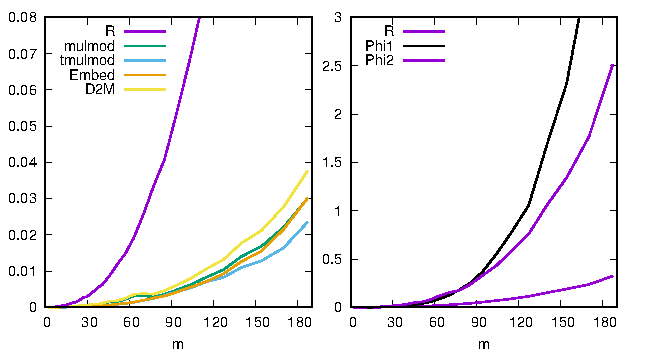
\includegraphics[width=0.8\textwidth]{ff_compositum/creat}
%  \vspace{-6ex}
  \caption{Timings in seconds, $p=5$, $n=m+1$}
  \label{ff_compositum:fig:bench}
%\vspace{-4ex}
\end{figure}

To demonstrate the practicality of our algorithms, we made a C
implementation and compared it to various ways of constructing the
same fields in Magma. All timings in this section are obtained on an
Intel Xeon E5620 CPU at 2.40GHz, using Magma V2.18-12, Flint 2.4.1 and
Sage 6.

Our implementation is limited to finite fields of word-sized
characteristic.  It is based on the C library
Flint~\cite{Hart2010}, and we make it available as a Sage module
in an experimental fork at
\url{https://github.com/defeo/sage/tree/ff_compositum}. We plan to
make it available as a standard Sage module, as well as a separate C
library, when the code has stabilized.

Based on the observation that algorithms {\sf Embed} and {\sf Project}
are simpler than conversion algorithms between monomial and dual
bases, we chose to implement a \emph{lazy change of basis}
strategy. By this we mean that our Sage module (rather than the C
library itself) represents elements on either the monomial or the dual
basis, with one representation computed from the other only when
needed. For example, two elements of the same field can be summed if
both have a monomial or if both have a dual representation. Similarly,
two elements can be multiplied using standard multiplication if both
have a monomial representation, or using transposed multiplication if
one of the two has a monomial representation. In all other cases, the
required representation is computed and stored when the user input
prompts it. To implement this strategy efficiently, our Sage module is
written in the compiled language Cython.

We focus our benchmarks on the setting of Section \ref{ff_compositum:sec:emb-iso}:
$P$ and $Q$ are two irreducible polynomials of coprime degrees $m$ and
$n$, and $R=P\odot Q$. We fix the base field $\F_p$ and make $m$ and
$n$ grow together with $n=m+1$. We measure the time to compute $R$, to
apply the algorithms {\sf Embed}, {\sf Phi1}, etc., and to compute the
changes of bases. We noticed no major difference between different
characteristics, so we chose $p=5$ for our demonstration. As shown in
Figure~\ref{ff_compositum:fig:bench}, the dominating phase is the computation of $R$
(line labeled {\sf R}). Surprisingly, transposed modular
multiplication is slightly faster than ordinary modular
multiplication. The cost of {\sf Embed} is about the same as that of
multiplication, while {\sf DualToMonomial} is about 50\% slower. {\sf
  Project} and {\sf MonomialToDual} have, respectively, similar
performances (only slightly faster) hence they are not reported on the
graph. This justifies our design choice of \emph{lazy change of
  basis}.  

Unsurprisingly, the isomorphism algorithms take significantly more
time than the computation of $R$; for our choices of degrees, {\sf
  Phi2} is asymptotically faster than {\sf Phi1} and the crossover
between them happens around $m=70$. 

\begin{figure}
  \centering
  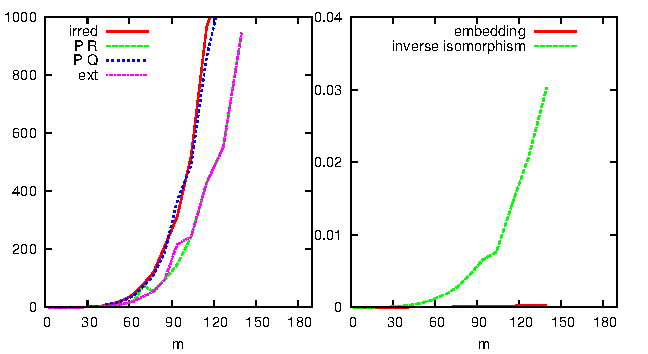
\includegraphics[width=0.8\textwidth]{ff_compositum/magma}
%  \vspace{-6ex}
\caption{Magma timings in seconds, $p=5$, $n=m+1$}
  \label{ff_compositum:fig:magma}
%\vspace{-4ex}
\end{figure}

We compare our implementation to four different strategies available
in Magma. For each of them we measure the time to construct the finite
fields and embedding data, as well as the time to do operations
equivalent to {\sf Embed}, resp.\ inverse
isomorphism. 

Figure~\ref{ff_compositum:fig:magma} reports on the following experiments.
In {\sf irred}, we supply directly $P$, $Q$ and $R$ to Magma's
  finite field constructor, then we call the \verb+Embed+ routine to
  compute the embedding data.
 In  {\sf P R}, we use Magma's default constructor to compute $P$
  and $R$ (Magma chooses its own polynomials), then we call the
  \verb+Embed+ routine to compute the embedding.
 In {\sf P Q}, we use Magma's default constructor to compute $P$
  and $Q$ (Magma chooses its own polynomials), then use the
  \verb+CommonOverfield+ routine to compute $R$, then \verb+Embed+ to
  compute the embedding data.
 In {\sf ext}, we use Magma's default constructor to compute $P$,
  then the \verb+ext+ operator to compute an extension of degree $n$
  of $\F_p[x]/\ang{P}$ (Magma chooses its own polynomials).


Timings for constructing the extension and the embedding vary from one
method to the other; once this is done, timings for applying
embeddings or (inverse) isomorphisms are the same across these
methods.

The Magma implementation cannot construct the embedding data in large
cases ($m = 150$) in less than 1000 seconds, while our code takes a
few seconds. Once the embedding data is known, Magma can apply the
embeddings or isomorphisms extremely fast; in our case, one may do the
same, using our algorithms to compute the matrices of $\Phi$ and
$\Phi^{-1}$, when precomputation time and memory are not a concern.

% \scriptsize
% \bibliographystyle{plain} \bibliography{defeo}




% Local Variables:
% ispell-local-dictionary:"american"
% End:

% LocalWords:  embeddings bilinear
}
{% \usepackage{graphicx}              
% \usepackage{amssymb}
% \usepackage{mathrsfs}
% \usepackage{url}
% \usepackage{hyperref}
% \usepackage{tikz}
% \usetikzlibrary{positioning,calc,arrows}
% \usepackage{algorithmic}
% \usepackage{subcaption}
% \usepackage{enumitem}

% theorem environments
% \theoremstyle{plain}
% \newtheorem{theorem}{Theorem}
% \newtheorem{lemma}[theorem]{Lemma}
% \newtheorem{corollary}[theorem]{Corollary}
% \newtheorem{proposition}[theorem]{Proposition}
% \theoremstyle{definition}
% \newtheorem{definition}[theorem]{Definition}
% \newtheorem{conjecture}[theorem]{Conjecture}
% \newtheorem*{problem}{Problem}
% \newtheorem{example}[theorem]{Example}
% \newtheorem*{remark}{Remark}
% \newtheorem{note}[theorem]{Note}

% \newcommand{\wrt}{\vdash} 
% \newcommand{\ang}[1]{\langle#1\rangle}
\newcommand{\abs}[1]{\left\vert#1\right\vert}
% \newcommand{\dual}[1]{\overline{#1}}
% \newcommand{\mapsfrom}{\ensuremath{\reflectbox{$\mapsto$}}}
% \newcommand{\tildO}{\tilde{O}}
% % roman numerals
% \newcommand{\romnum}[1]{\romannumeral #1}
% \newcommand{\Romnum}[1]{\uppercase\expandafter{\romannumeral #1}}

% \newcommand{\todo}[1]{\textcolor{red}{TODO: #1}}
% \newcommand{\comment}[2][Note]{\textcolor{green}{(#1): #2}}

% \DeclareMathOperator{\fieldchar}{char} % characteristic of a field
% \DeclareMathOperator{\ringofend}{End} % endomorphism ring
\let\trace\Tr
% \DeclareMathOperator{\trace}{Tr} % finite field trace
\let\gal\Gal % Galois group
\let\order\ord % order of an element
% \DeclareMathOperator{\lcm}{lcm} % least common multiple
% \DeclareMathOperator{\divisor}{div} % divisor on a curve
% \DeclareMathOperator{\supp}{supp} % support of a divisor
% \DeclareMathOperator{\norm}{N} % norm
% \DeclareMathOperator{\Res}{Res}
% \DeclareMathOperator{\Aut}{Aut}
% \DeclareMathOperator{\minpoly}{minpoly}
% \DeclareMathOperator{\loglog}{loglog}
% \DeclareMathOperator{\rev}{rev}

\newcommand{\Q}{\ensuremath{\mathbb{Q}}}
% \newcommand{\N}{\ensuremath{\mathbb{N}}}
% \newcommand{\R}{\ensuremath{\mathbb{R}}}
\newcommand{\Z}{\ensuremath{\mathbb{Z}}}
% \newcommand{\F}{\ensuremath{\mathbb{F}}}
\newcommand{\MM}{\ensuremath{\mathsf{M}}}
% \newcommand{\euler}{\ensuremath{\varphi}}

% allow algorithms to split over multiple pages
% \makeatletter
% \newcounter{algorithm}
% \setcounter{algorithm}{0}
% \renewcommand{\thealgorithm}{\arabic{algorithm}}
% \def\algorithm{\@ifnextchar[{\@algorithma}{\@algorithmb}}
% \def\@algorithma[#1]{%
% 	\refstepcounter{algorithm}
% 	\trivlist
% 	\leftmargin\z@
% 	\itemindent\z@
% 	\labelsep\z@
% 	\item[\parbox{\columnwidth}{%
% 		\hrule
% 		\hrule
% 		\noindent\strut\textbf{Algorithm \thealgorithm} #1
% 		\hrule
% 	}]\hfil\vskip0em%
% }
% \def\@algorithmb{\@algorithma[]}
% \def\endalgorithm{\hfil\vskip-1em\hrule\endtrivlist}
% \makeatother

%%%%%%%%%%%%%%%%%%%%%%%%%%%%%%%%%%%%%%%%%

\chapter{Computing isomorphisms and embeddings of finite fields}

% \author[L. Brieulle]{Ludovic Brieulle}
% \address{Laboratoire de Math\'ematiques de Versailles,
%   UVSQ, CNRS, Universit\'e Paris-Saclay}

% \author[L. De Feo]{Luca De Feo}
% \address{Laboratoire de Math\'ematiques de Versailles,
%   UVSQ, CNRS
%   \& Inria, Universit\'e Paris-Saclay}
% \email{luca.de-feo@uvsq.fr}
% \email{http://orcid.org/0000-0002-9321-0773}

% \author[J. Doliskani]{Javad Doliskani}
% \address{Institute for Quantum Computing, University of Waterloo}
% \email{javad.doliskani@uwaterloo.ca}

% \author[J.-P. Flori]{Jean-Pierre Flori}
% \address{Agence nationale de la s\'ecurit\'e des syst\`emes d'information}

% \author[\'E. Schost]{\'Eric Schost}
% \address{Cheriton School of Computer Science, University of Waterloo}


\begin{abstract}
  Let $\F_q$ be a finite field. %
  Given two irreducible polynomials $f,g$ over $\F_q$, with $\deg f$
  dividing $\deg g$, the finite field embedding problem asks to
  compute an explicit description of a field embedding of
  $\F_q[X]/f(X)$ into $\F_q[Y]/g(Y)$. %
  When $\deg f = \deg g$, this is also known as the isomorphism
  problem.

  This problem, a special instance of polynomial factorization, plays
  a central role in computer algebra software. %
  We review previous algorithms, due to Lenstra, Allombert, Rains, and
  Narayanan, and propose improvements and generalizations. %
  Our detailed complexity analysis shows that our newly proposed
  variants are at least as efficient as previously known algorithms,
  and in many cases significantly better.

  We also implement most of the presented algorithms, compare them
  with the state of the art computer algebra software, and make the
  code available as open source. %
  Our experiments show that our new variants consistently outperform
  available software.
\end{abstract}


%%%%%%%%%%%%%%%%%%%%%%%%%%%%%%%%%%
%%%%%%%%%%%%%%%%%%%%%%%%%%%%%%%%%%


\section{Introduction}
\label{sec:introduction}

Let $q$ be a prime power and let $\F_q$ be a field with $q$
elements. Let $f$ and $g$ be irreducible polynomials over $\F_q$, with
$\deg f$ dividing $\deg g$. Define $k=\F_q[X]/f(X)$ and
$K=\F_q[Y]/g(Y)$; then, there is an embedding $\phi:k\hookrightarrow
K$, unique up to $\F_q$-automorphisms of $k$. The goal of this paper
is to describe algorithms to efficiently represent and evaluate one
such embedding.

All the algorithms we are aware of split the embedding problem in two
sub-problems:
\begin{enumerate}
\item Determine elements $\alpha\in k$ and $\beta\in K$ such that
  $k=\F_q(\alpha)$, and such that there exists an
  embedding $\phi$ mapping $\alpha$ to $\beta$. We refer to this
  problem as the \emph{embedding description problem}.
  It is easily seen that $(\alpha,\beta)$ describes an embedding
  if and only if $\alpha$ and $\beta$ share the same minimal polynomial.
\item Given elements $\alpha$ and $\beta$ as above, given $\gamma\in
  k$ and $\delta\in K$, solve the following problems:
  \begin{itemize}
  \item Compute $\phi(\gamma)\in K$.
  \item Test if $\delta\in\phi(k)$.
  \item If $\delta\in\phi(k)$, compute $\phi^{-1}(\delta)\in k$.
  \end{itemize}
  We refer collectively to these problems as the \emph{embedding
    evaluation problem}.
\end{enumerate}


\paragraph{\bf Motivation, previous work.}
The first to get interested in this problem was H.~Lenstra: in his
seminal paper~\cite{LenstraJr91} he shows that it can be solved in
deterministic polynomial time, by using a representation for finite
fields that he calls \emph{explicit data}.\footnote{Technically,
  Lenstra only proved his theorem in the case where $k$ and $K$ are
  isomorphic; however, the generalization to the embedding problem
  poses no difficulties.} %
In practice, the embedding problem arises naturally when designing a
computer algebra system: as soon as a system is capable of
representing arbitrary finite fields, it is natural to ask it to
compute the morphisms between them. %
Ultimately, by representing effectively the lattice of finite fields
with inclusions, the user is given access to the algebraic closure of
$\F_q$. %
The first system to implement a general embedding algorithm was
Magma~\cite{MAGMA}. %
As detailed by its developers~\cite{bosma+cannon+steel97}, it used a
much simpler approach than Lenstra's algorithm, entirely based on
polynomial factorization and linear algebra. %
Lenstra's algorithm was later revived by
Allombert~\cite{Allombert02,Allombert02-rev} who modified some key
steps in order to make it practical; his implementation has since been
part of the PARI/GP system~\cite{Pari}.

Meanwhile, a distinct family of algorithms for the embedding problem
was started by Pinch~\cite{Pinch}, and later improved by
Rains~\cite{rains2008}. %
These algorithms, based on principles radically different from
Lenstra's, are intrinsically probabilistic. %
Although their worst-case complexity is no better than that of
Allombert's algorithm, they are potentially much more efficient on a
large set of parameters. %
This potential was understood by Magma's developers, who implemented
Rains' algorithm in Magma v2.14.%
\footnote{As a matter of fact, Rains' algorithm was never published;
  the only publicly available source for it is in Magma's source code
  (file \texttt{package/Ring/FldFin/embed.m}, since v2.14).}

With the exception of Lenstra's work, the aforementioned papers were
mostly concerned with the practical aspects of the embedding
problem. %
While it was generally understood that computing embeddings is an
easier problem than general polynomial factoring, no results on its
complexity more precise than Lenstra's had appeared until recently. %
A few months before the present paper was finalized, Narayanan
published a novel generalization of Allombert's
algorithm~\cite{narayanan2016fast}, based on elliptic curve
computations, and showed that its (randomized) complexity is at most
quadratic.
Narayanan's
  generalization relies on the fact that Artin--Schreier and Kummer
  theories are special cases of a more general situation:
  as already emphasized by Couveignes and Lercier~\cite{CL08}, whereas
  the former theory acts on the additive group of a finite field, and
  the latter on its multiplicative group, they can be extended to more
  general commutative algebraic groups, in particular to elliptic
  curves.

\paragraph{\bf Our contribution.}
This work aims to be, in large part, a complete review of all known
algorithms for the embedding problem; we analyze in detail the cost of 
existing algorithms and introduce several new variants. %
After laying out the foundations in the next section, we start with
algorithms for the embedding description problem. %

Section~\ref{sec:kummer} describes the family of algorithms based
(more or less loosely) on Lenstra's work; we call these
\emph{Kummer-type} algorithms. %
In doing so, we pay a particular attention to Allombert's algorithm:
to our knowledge, this is the first detailed and complete complexity
analysis of this algorithm and its variants. %
Thanks to our work on asymptotic complexity, we were able to devise
improvements to the original variants of Allombert that largely
outperform them both in theory and practice. %
One notable omission in this section is Narayanan's algorithm, which
is, in our opinion, mostly of theoretical rather than practical
interest. %
We present instead in Subsection~\ref{sec:fast-algor-large} a simpler
algorithm with essentially the same complexity.

In Section~\ref{sec:rains-algorithm} we describe Rains' algorithm. %
Rains' original preprint~\cite{rains2008} went unpublished, thus we
give here a complete description and analysis of his algorithm, for
reference. %
We also give new variants of Rains' algorithm of lesser
interest in Appendix~\ref{app:rains-vars}.

Then, in Section~\ref{sec:rains-elliptic} we present a generalization
of Rains' algorithm using elliptic curves. %
The possibility of this algorithm was hinted at by Rains, but never
fully developed; we show that it is indeed possible to use
\emph{elliptic periods} to solve the embedding description problem,
and that the resulting algorithm behaves well both in theory and in
practice. %
While working out the correctness proof of the elliptic variant of
Rains' algorithm, we encounter an unexpected difficulty: whereas roots
of unity enjoy Galois properties that guarantee the success of Rains'
original algorithm, points of elliptic curves fail to provide the
same. %
Heuristically, the failure probability of the elliptic variant is
extremely small, however we are not able to prove it formally. %
Our experimental searches even seem to suggest that the failure
probability might be, surprisingly, zero. %
We state this as a conjecture on elliptic periods (see
Conjecture~\ref{conj:ellperiods}).

Section~\ref{sec:selection} does a global comparison of all the
algorithms presented previously. %
In particular, Rains' algorithm and variants require a non-trivial
search for parameters, which we discuss thoroughly. %
Then we present an algorithm to select the best performing embedding
description algorithm from a practical point of view. %
This theoretical study is complemented by the experimental
Section~\ref{sec:experimental-results}, where we compare our
implementations of all the algorithms; our source code is made
available through the Git repository
\url{https://github.com/defeo/ffisom} for replication and further
scrutiny.

The algorithms for the embedding evaluation problem are much more
classical and well understood. %
Due to space constraints, we do not present them here; we address
instead the interested reader to the extended version of the present
paper~\cite{ffisom-long}.

In conclusion, we hope that our review will constitute a reference
guide for researchers and engineers interested in implementing
embeddings of finite fields in a computer algebra system.


\section{Preliminaries}
\label{sec:preliminaries}

\subsection{Fundamental algorithms and complexity}
\label{sec:fundamentalgo}
We review the fundamental building blocks that constitute the
algorithms presented next.  We are going to measure all complexities
in number of operations $+$, $\times$, $\div$ in $\F_q$, unless
explicitly stated otherwise. Most of the algorithms we present are
randomized; we use the \emph{big-Oh} notation $O(\,)$ to express {\em average}
asymptotic complexity, and we will make it clear when this complexity
depends on heuristics. We also occasionally use the notation
$\tildO(\,)$ to neglect logarithmic factors in the parameters.

We let $\MM(m)$ be a function such that polynomials in $\F_q[X]$ of
degree less than $m$ can be multiplied in $\MM(m)$ operations in
$\F_q$, under the assumptions of~\cite[Ch.~8.3]{vzGG}, together with
the slightly stronger one, that $\MM(mn)$ is in $O(m^{1+\varepsilon}
\MM(n))$ for all $\varepsilon > 0$. Using FFT multiplication, one can
take $\MM(m)\in O(m\log(m) \loglog(m))$~\cite{cantor+kaltofen91}.

We denote by $\omega$ the \emph{exponent of linear algebra}, i.e.\ a
constant such that $m\times m$ matrices with coefficients in any field
$k$ can be multiplied using $O(m^\omega)$ additions and
multiplications in $k$. One can take $\omega < 2.38$, the best result
to date being in~\cite{LeGall14}; on the other hand, we also suppose
that $\omega > 2$.

The algorithms presented in the next sections perform computations in
ring extensions of finite fields. Some of these extensions also happen
to be finite fields. As customary, if $k$ is a finite field and $\xi$
is some element of an algebraic extension of $k$, we will write
$k[\xi]$ for the ring generated by $\xi$. To avoid confusion, when the
extension generated by $\xi$ is a finite field, we will write instead
$k(\xi)$.

Some algorithms will operate in a polynomial ring $k[Z]$, where $k$ is
a field extension of $\F_q$; some other algorithms will operate in
$k[Z]/h(Z)$, where $h$ is a monic polynomial in $k[Z]$. We review the
basic operations in these rings. We assume that $k$ is represented as
a quotient ring $\F_q[X]/f(X)$, with $m=\deg f$, and we let $s=\deg h$
in the complexity estimates.

Multiplying and dividing polynomials of degree at most $s$ in $k[Z]$
is done in $O(\MM(sm))$ operations in $\F_q$, using Kronecker's
substitution~\cite{moenck76,kaltofen87,vzGG,von1992computing,harvey09}.
Multiplication in $k[Z]/h(Z)$ is also done in $O(\MM(sm))$ operations using the
technique in~\cite{pascal+schost06}. By the same techniques, gcds of
degree $m$ polynomials in $k[Z]$ and inverses in $k[Z]/h(Z)$ are
computed in $O(\MM(sm)\log(sm))$ operations.

Given polynomials $e,g,h \in k[Z]$ of degree at most $s$, modular
composition is the problem of computing $e(g) \bmod h$. An upper bound
on the algebraic complexity of modular composition is obtained by the
Brent--Kung algorithm~\cite{brent+kung}; under our assumptions on the
respective costs of polynomial and matrix multiplication, its cost is
$O(s^{(\omega+1)/2}\MM(m))$ operations in $\F_q$
(so if $k=\F_q$, this is $O(s^{(\omega+1)/2})$). In the binary RAM
complexity model, the Kedlaya--Umans algorithm~\cite{KeUm11} and its
extension in~\cite{PoSc13a} yield an algorithm with essentially linear
complexity in $s$, $m$ and $\log(q)$. Unfortunately, making these
algorithms competitive in practice is challenging; we are not aware of
any implementation of them that would outperform Brent and Kung's
algorithm. 

\begin{note}\label{note:multimc}
If we have several modular compositions of the form $e_1(g) \bmod
h,\dots,$ $e_t(g) \bmod h$ to compute, we can slightly improve the obvious
bound $O(ts^{(\omega+1)/2})$ (we discuss here $k=\F_q$, so $m=1$). If
$t=O(s)$, using~\cite[Lemma~4]{kaltofen+shoup98}, this can be done in
time $O(t^{(\omega-1)/2}s^{(\omega+1)/2})$. If $t=\Omega(s)$, this can
be done in $O(t s^{\omega-1})$ operations, by computing $1,g,\dots,g^{s-1}$
modulo $f$, and doing a matrix product in size $s \times s$ by
$s \times t$.
\end{note}

\paragraph{\bf Frobenius evaluation.} Consider an $\F_q$-algebra $Q$,
and an element $\alpha$ in $Q$. Given integers $c,d$, we will have to
compute expressions of the form
\[
\sigma_d= \alpha^{q^d}, \quad \tau_d = \sum_{i=0}^{d-1} \alpha^{q^{ci}}, \quad
\mu_d=\alpha^{\lfloor q^d/c\rfloor} \enspace .
\]
A direct binary powering approach
would yield a complexity of, e.g., $O(d\log(q))$ multiplications in $Q$
for the first expression.

To do better, we use a recursive approach that goes back
to~\cite{von1992computing}, with further ideas borrowed from~\cite{shoup94,kaltofen+shoup97}.
For $i \ge 1$, define integers $A_i, B_i$ as follows
\begin{equation*}
  q^i = A_ic + B_i, \quad 0\le B_i < c.
\end{equation*}
Then, we have the relations
$$\sigma_{i+j}=\sigma_j^{q^i}, \quad \tau_{i+j}=\tau_i +
\tau_j^{q^{ic}}, \quad \mu_{i+j}=\mu_j^{q^i}
\mu_i^{B_j}\alpha^{\lfloor B_iB_j / c \rfloor}.$$ Since we are
interested in $\sigma_d,\tau_d$ and $\mu_d$, using an addition chain
for $d$, we are left to perform $O(\log(d))$ steps as above.

To perform these operations, we will make a heavy use of a technique
originating in~\cite{von1992computing}. In its simplest form, it
amounts to the following: if $Q=\F_q[X]/f(X)$, for some polynomial $f$
in $\F_q[X]$, and $\beta$ is in $Q$, we can compute $\beta^{q}$ by
means of the modular composition $\beta(\xi)$, where $\xi = x^{q}$ and
$x$ is the image of $X$ modulo $f$.

In the following proposition, we discuss
versions of this idea for various kinds of algebras $Q$, and how they
allow us to compute the expressions $\sigma_d, \tau_d, \mu_d$ defined
above.

\begin{proposition}
\label{prop:trace-like}
Let $f \in \F_q[X]$ be a polynomial of degree $m$,
and define the $\F_q$-algebra $Q = \F_q[X]/f(X)$.
Let $h \in Q[Z]$ be a polynomial of degree $s$,
and define the $Q$-algebra $S =  Q[Z]/h(Z)$.
Finally, whenever $h \in \F_q[Z]$, define
the $\F_q$-algebra $Q' = \F_q[Z]/h(Z)$.

Denote by $T_Q, T_S, T_{Q'}$ the cost, in terms of $\F_q$-operations,
of one modular composition in $Q, S, Q'$ respectively. %
Also denote by $T_{Q,t}\le tT_Q$ (resp. $T_{S,t}, T_{Q',t}$) the cost of $t$
modular compositions sharing the same polynomial (see
Note~\ref{note:multimc}).

Then the expressions
\[
\sigma_d= \alpha^{q^d}, \quad \tau_d = \sum_{i=0}^{d-1} \alpha^{q^{ci}}, \quad
\mu_d=\alpha^{\lfloor q^d/c\rfloor}
\]
can be computed using the following number of operations:
\begin{enumerate}[label=\textbf{Case~\theenumi.},leftmargin=*, align=left]
\item $\alpha \in Q$:
\begin{itemize}
\item
$\sigma_d$: $O(\MM(m) \log(q) + T_Q \log(d))$,
\item
$\tau_d$: $O(\MM(m) \log(q) + T_Q \log(d c))$,
\item
$\mu_d$: $O(\MM(m) \log(q) + (T_Q + \MM(m)\log(c))\log(d))$;
\end{itemize}
\item $\alpha \in Q$ with $f | X^r - 1$:
\begin{itemize}
\item
$\sigma_d$: $O(\MM(m) \log(q) + \MM(r) \log(d))$,
\item
$\tau_d$: $O(\MM(m) \log(q) + \MM(r) \log(d c))$,
\item
$\mu_d$: $O(\MM(m) \log(q) + (\MM(r) + \MM(m)\log(c))\log(d))$;
\end{itemize}
\item $\alpha \in S$:
\begin{itemize}
\item
$\sigma_d$: $O(\MM(ms)\log(q) + (T_{Q,s}+T_S)\log(d))$,
\item
$\tau_d$: $O(\MM(ms)\log(q) + (T_{Q,s}+T_S)\log(d c))$,
\item
$\mu_d$: $ O(\MM(ms)\log(q) + (T_{Q,s}+T_S + \MM(ms)\log(c))\log(d))$;
\end{itemize}
\item $\alpha \in S$ with $h \in \F_q[Z]$:
\begin{itemize}
\item
$\sigma_d$: $O((\MM(m)+\MM(s))\log(q) + (T_{Q,s}+T_{Q',m})\log(d)$,
\item
$\tau_d$: $O((\MM(m)+\MM(s))\log(q) + (T_{Q,s}+T_{Q',m})\log(d c))$,
\item
$\mu_d$: $O((\MM(m)+\MM(s))\log(q) + (T_{Q,s}+T_{Q',m} + (m\MM(s)+s\MM(m))\log(c))\log(d))$;
\end{itemize}
\item $\alpha \in S$ with $h | X^r - a$ for $a \in Q$:
\begin{itemize}
\item
$\sigma_d$: $O(\MM(m)\log(q) + (T_{Q,s}+ \MM(mr))\log(d))$,
\item
$\tau_d$: $O(\MM(m)\log(q) + (T_{Q,s} + \MM(mr))\log(d c))$,
\item
$\mu_d$: $O(\MM(m)\log(q) + (T_{Q,s} + \MM(mr) + \MM(m)\log(c))\log(d))$.
\end{itemize}
\end{enumerate}
\end{proposition}

\begin{proof}
The complexity estimates mostly rely on the complexity of modular composition.
\begin{enumerate}[label=\textbf{Case~\theenumi.},leftmargin=*, align=left]
\item
  We let $x$ be the image of $X$ in $Q$, and we
  start by computing $x^q$, using $O(\MM(m)\log(q))$ operations in
  $\F_q$.

  For $i \ge 0$, given $\xi_i = x^{q^i}$ and $\beta$ in $Q$, we can
  compute $\beta^{q^i}$ as $\beta^{q^i}=\beta(\xi_i)$, using
  $T_Q=O(m^{(\omega+1)/2})$ operations; in particular, this allows us to
  compute $\xi_{i+j}$ from the knowledge of $\xi_i$ and $\xi_j$. Given
  an addition chain for $d$, we thus compute all corresponding
  $\xi_i$'s, and we deduce the $\sigma_i$'s similarly, since
  $\sigma_{i+j}=\sigma_j(\xi_j)$. Altogether, starting from
  $\xi_1=x^q$, this gives us $\sigma_d$ for $O(T_Q\log(d))$
  further operations in $\F_q$.

  The same holds for $\tau_d$, with a cost in $O(T_Q\log(cd))$,
  since we have to compute $\xi_c$ first;
  and for $\mu_d$, with a cost in
  $O((T_Q + \MM(m)\log(c))\log(d))$ operations,
  as the formula for $\mu_{i+j}$ shows that
  we can obtain it by means of a modular composition
  (to compute $\mu_j^{q^i}=\mu_j(\xi_i)$), together with
  two exponentiations of indices less than~$c$.

  The costs for computing $\sigma_d, \tau_d, \mu_d$ follow immediately.

\item
  When $f$ divides $X^r-1$, we obtain $\beta(\xi_i)$ by computing
  $\beta(X^{q^i \bmod r}) \bmod (X^r-1)$ first, and then reducing
  modulo $f(X)$.  %
  Thus, the cost of one modular composition is $T_Q=O(\MM(r))$, and
  the total cost is obtained by replacing this value in the estimates
  for the previous case.

\item
  We let $x$ and $z$ be the respective images of $X$ in $Q$ and $Z$ in $S$,
  and as a first step, we compute $z^q$ (and $x^q$, unless $f$ is as
  in Case~2 above), in $O(\MM(ms)\log(q))$ operations.
  
  In order to compute
  the quantities $\sigma_d,\tau_d,\mu_d$, we apply the same strategy
  as above; the key factor for complexity is thus the cost of
  computing $\beta^{q^i}$, for $\beta$ in $S$, given $\zeta_i =
  z^{q^i}$ and $\xi_i=x^{q^i}$ (as we did in Case~1, we apply this
  procedure to our input element $\alpha$, as well as to $\zeta_i$
  itself, and $\xi_i$, in order to be able to continue the
  calculation).

  To do so, we use an algorithm by Kaltofen and Shoup~\cite{kaltofen+shoup97},
  which boils down to writing $\beta=\sum_{j=0}^{s-1} c_j(x) z^j$, so
  that $\beta^{q^i} = \sum_{j=0}^{s-1} c_j(x)^{q^i} \zeta_i^j.$ The
  $s$ coefficients $c_j(x)^{q^i}$ are computed by applying the
  previous algorithms in $Q$ to $s$ inputs. This takes time at most
  $sT_Q$, but as pointed out in Note~\ref{note:multimc}, improvements 
  are possible if we base our algorithm on modular composition;
  we thus denote the cost $T_{Q,s}$.

  Then, we do a modular composition in $S$ to evaluate the result at
  $\zeta_i$; this latter step takes $T_S=O(s^{(\omega+1)/2} \MM(m))$
  operations in~$\F_q$.

\item
  The cost for computing $z^q$ is
  $O(\MM(s)\log(q))$ and that for computing $x^q$ is $O(\MM(m)\log(q))$.
  In the last step, the cost $T_S$ of modular
  composition in $S$ is now that of $m$ modular compositions in degree
  $s$ (with the same argument), as detailed in
  Note~\ref{note:multimc}, that we denote $T_{Q',m}$.
  Similarly, the cost of multiplication in $S$ can be reduced
  from $O(\MM(ms))$ to $O(s\MM(m) + m\MM(s))$ operations.

\item
  We start by computing $x^q$, using $O(\MM(m)\log(q))$ operations in
  $\F_q$.

  For $\beta$ as above, suppose that we have already computed all
  coefficients $d_j(x)=c_j(x)^{q^i}$ in $O(T_{Q,s})$ operations;
  we now have to compute $\beta^{q^i} = \sum_{j=0}^{s-1} d_j(x) \zeta_i^j$.

  We first do the calculation modulo $Z^r-a$ rather than modulo $h$;
  that is, we compute $\sum_{j=0}^{s-1} d_j(x) z_i^j$ where
  $z_i=z^{q^i}$.
  Because $z^r=a$, we
  have $z_i = a_i z^{q^i \bmod r}$, with $a_i =
  a^{\lfloor q^i/r\rfloor}$. If we assume that $a_i$ is
  known, we can compute $\sum_{j=0}^{s-1} d_j(x) z_i^j$ using
  Horner's method, in time $O(s \MM(m))$, and we reduce this result
  modulo $h$, for the cost $O(\MM(mr))$ of a Euclidean division in
  degree $r$ in $Q[Z]$. 

  In order to continue the calculation for all indices in our addition
  chain, we must thus compute the corresponding $a_i$'s as well,
  just like the $\mu_i$'s;
  this takes $O(T_{Q}+\MM(m)\log(r))$ operations.

  Since the first stage of the algorithm took $O(T_{Q,s})$ operations,
  we can take $T_S = O(\MM(mr))$
  for computing $\beta^{q^i}$.
  
  To initiate the procedure, the algorithm also needs to compute
  $a_1=a^{\lfloor q/r\rfloor}$, using $O(\log(q))$
  multiplications in $Q$ for a cost $O(\MM(m)\log(q))$. \qedhere
\end{enumerate}
\end{proof}

\paragraph{\bf Computing subfields.}
With $k = \F_q[X]/f(X)$ and $\deg f=m$ as above, we are given a
divisor $r$ of $m$, and we want to construct an intermediate extension
$\F_q \subset L \subset k$ of degree $r$ over $\F_q$. More precisely,
we want to compute a monic irreducible polynomial $g \in \F_q[X]$ of
degree $r$, and a polynomial $h \in \F_q[X]$ such that
$x \mapsto h(x)\bmod f$ defines an embedding
$L = \F_q[X] / g(X) \hookrightarrow k$.

An algorithm for this will be used to reduce the embedding problem to
an isomorphism problem; although this is not strictly necessary for
most of our algorithms to work, it will greatly simplify the
expostion. We proceed as follows.

Let $\alpha\in k$ be a random element\footnote{For efficiency reasons,
  it may be preferable to choose $\alpha$ pseudo-randomly, such as a
  low-degree polynomial in the generator of $k$}. %
Then $\alpha$ has a minimal polynomial of degree $m$ 
over $\F_q$ with high probability. In other words, one needs $O(1)$ such random elements to find 
one with degree $m$ minimal polynomial. Now, the trace
\begin{equation}
	\label{equ:trace-simple}
	\trace_{k/L}(\alpha) = \alpha + \alpha^{q^r} + \cdots + \alpha^{q^{m - r}}
\end{equation}
has a minimal polynomial of degree $r$ over $\F_q$ with high
probability as well. This means we can compute, after $O(1)$ random
trials, the desired polynomials $\beta = \trace_{k/L}(\alpha)$,
its minimal polynomial
$g$, and $h$ the polynomial of degree less than $m$ representing $\beta$.

\begin{proposition}
	\label{prop:subfield}
	Let $\F_q \subset k$ be a finite extension of degree $m$, and
        let $r$ be a divisor of $m$.  Computing an intermediate field
        $\F_q \subset L \subset k$ with $[L:\F_q]=r$ takes an expected
        $O(m^{(\omega+1)/2}\log(m) + \MM(m)\log(q))$ operations in $\F_q$.  Once
        $L$ is computed, any element $\gamma\in L$ can be lifted to
        its image in $k$ using $O(m^{(\omega+1)/2})$ operations.
\end{proposition}
\begin{proof}
  Computing the minimal polynomial of an element in $k$ takes
  $O(m^{(\omega+1)/2})$ operations in $\F_q$, see~\cite{shoup99}. %
  The trace in Eq.~\eqref{equ:trace-simple} is computed as the
  expression $\tau_m$ of the previous paragraph (with $c=r$ and
  $d=m/r$), at a cost of $O(m^{(\omega+1)/2}\log(m)+\MM(m)\log(q))$
  operations in $\F_q$.
  
  Finally, given an element $\gamma\in L$, its image in $k$ is
  computed by evaluating $h(\gamma)$, where $h$ is the polynomial
  representation of $\trace_{k/L}(\alpha)$. This can be done by a
  modular composition at cost $O(m^{(\omega+1)/2})$.
\end{proof}

\paragraph{\bf Root finding in cyclotomic extensions.}
Given a field $k = \F_q[X]/f(X)$ of degree $m$ as above, we will need
to factor some special polynomials in $k[Z]$: we are interested in
finding one factor of a polynomial that splits into factors of the
same, known, degree. This problem is known as \emph{equal degree
  factorization} (EDF), and the best generic algorithm for it is the
Cantor--Zassenhaus method~\cite{cantor1981,von1992computing}, which
runs in $O(\MM(sm)(dm\log(q) + \log(sm)))$ operations in
$\F_q$~\cite[Th.~14.9]{vzGG}, where $s$ is the degree of the
polynomial to factor, and $d$ is the degree of the factors.

More efficient variants of the Cantor--Zassenhaus method are known for
special cases. When the degree $s$ of the polynomial is small compared
to the extension degree $m$, Kaltofen and Shoup~\cite{kaltofen+shoup97} 
give an efficient algorithm which is as follows.

\begin{algorithm}
  \caption{Kaltofen--Shoup EDF for extension fields}
	\label{alg:ks}
	\begin{algorithmic}[1]
		\REQUIRE A polynomial $h$  with irreducible factors of degree $d$ over $k=\F_q[X]/f(X)$.
		\ENSURE An irreducible factor of $h$ over $k$.
		\STATE If $\deg h = d$ return $h$.
		\STATE Take a random polynomial $a_0\in k[Z]$ of degree less than $\deg h$,
		\STATE\label{alg:ks-pseudotrace} Compute $\displaystyle a_1 
		\leftarrow \sum_{i=0}^{md-1} a_0^{q^i} \mod h$,
		\IF{$q$ is an even power $q=2^e$}
		\STATE\label{alg:ks:even} Compute $\displaystyle a_2 \leftarrow 
		\sum_{i=0}^{e-1} a_1^{2^i}\mod h$
		\ELSE
		\STATE\label{alg:ks:odd} Compute $a_2 \leftarrow a_1^{(q-1)/2}\mod h$
		\ENDIF
		\STATE\label{alg:ks:gcd} Compute $h_0\leftarrow\gcd(a_2,h)$ and 
		$h_1\leftarrow\gcd(a_2-1,h)$ and $h_{-1}\leftarrow h/(h_0h_1)$,
		\STATE Apply recursively to the smallest non-constant polynomial among 
		$h_0,h_1,h_{-1}$.
	\end{algorithmic}
\end{algorithm}


We refer the reader to the original paper~\cite{kaltofen+shoup97} for
the correctness of the Kaltofen--Shoup algorithm. We are mainly
interested here in its application to root extraction in cyclotomic
extensions. Let $r$ be a prime power and let $f$ be an irreducible
factor of the $r$-th cyclotomic polynomial $\Phi_r$, with $s = \deg
f$. Denote $\F_q[X] / f(X)$ by $\F_q(\zeta)$, where $\zeta$ is the
image of $X$ in the quotient. Given an $r$-th power $\alpha \in
\F_q(\zeta)$ we want to compute an $r$-th root $\alpha^{1 / r}$, or
equivalently a linear factor of $Z^r - \alpha$ over $\F_q(\zeta)$.

We propose two different algorithms; one of them is quadratic in $r$,
whereas the other one has a runtime that depends on $r$ and $s$,
and will perform better for small values of $s$.

\begin{proposition}
  \label{prop:root-fpz}
  Let $r$ be a prime power and let $\zeta$ be a primitive $r$-th root of unity; let also $s = 
  [\F_q(\zeta): \F_q]$. One can take $r$-th roots in 
  $\F_q(\zeta)$ using either 
  $$O(\MM(s)\log(q) + rs^{\omega-1}\log(r)\log(s) + \MM(rs)\log(s)\log(r))$$
  or
  $$O(\MM(s)\log(q) + r\MM(r)\log(s) + \MM(rs)\log(s)\log(r))$$ operations in $\F_q$. 
\end{proposition}
\begin{proof}
We use Algorithm~\ref{alg:ks} with $k=\F_q(\zeta)$, to get a linear
factor of the polynomial $Z^r-\alpha$, so that $d=1$ (note that
$Z^r-\alpha$ splits into linear factors in $k[Z]$). We discuss
Step~\ref{alg:ks-pseudotrace}, which is the dominant step. Let $f \in
\F_q[X]$ be the defining polynomial of $\F_q(\zeta)$ and let $h$ be a
factor of $Z^r-\alpha$ of degree $n$. 

We are in Case~5 of our discussion on Frobenius evaluation, and we
want to compute a trace-like expression of the form $\tau_s$. As per
that discussion, two algorithms are available to do Frobenius
evaluation in $k$ (one of them uses modular composition, the other the
fact that $f$ divides $X^r-1$). Because $s \le r$, we deduce that
$a_1$ can be computed in either
$$O(\MM(s)\log(q) + rs^{\omega-1}\log(s) + \MM(rs)\log(s))$$
or
$$O(\MM(s)\log(q) + n\MM(r)\log(s) + \MM(rs)\log(s))$$ operations in
$\F_q$, where the first term accounts for computing $\alpha^{\lfloor
  q/r \rfloor}$ (so we need only compute it once).

Steps~\ref{alg:ks:odd} and~\ref{alg:ks:even} are again an instance of
Case~5, and their cost is subsumed by Step~\ref{alg:ks-pseudotrace}.
The depth of the recursion in Algorithm~\ref{alg:ks} is $\log(r)$, and
the degree $n$ is halved each time, so we obtain the desired result.
\end{proof}

\paragraph{\bf Root finding in some extensions of cyclotomic extensions.}
Let $r = v^d$, where $v \ne p$ is a prime and $d$ is a positive
integer and let $s$ be the order of $q$ in $\Z / v\Z$.  We 
assume that $d \ge 2$, since this will be the case whenever we want to
apply the following.

Consider an extension $\F_q \subset k=\F_q[X]/f(X)$ of degree $r$, and
let $\F_q(\zeta)$ and $k(\zeta)$ be extensions of degree $s$ over
$\F_q$ and $k$ respectively, defined by an irreducible factor of the
$v$-th cyclotomic polynomial over $\F_q$. In this paragraph, we
discuss the cost of computing a $v$-th root in $k(\zeta)$, by adapting
the root extraction algorithm given in~\cite{doliskanischost2011}.

Following~\cite[Algorithm~3]{doliskanischost2011}, one reduces the
root extraction in $k(\zeta)$ to a root extraction in $\F_q(\zeta)$;
note that \cite[Algorithm~3]{doliskanischost2011} reduces the root
extraction to the smallest possible extension of $\F_p$, but
projecting to $\F_q(\zeta)$ is more convenient here. The critical
computation in this algorithm is a trace-like computation performing
the reduction.

\begin{algorithm}
\caption{$v$-th root in $k(\zeta)$}
\label{algorithm:new}
\begin{algorithmic}[1]
\REQUIRE $a \in k(\zeta)^v$
\ENSURE a $v$-th root of $a$
\REPEAT
\STATE choose a random $c \in k(\zeta)$
\STATE $a'\leftarrow ac^v$
\STATE $\lambda \leftarrow {a'}^{(q^s-1)/v}$
\STATE $b \leftarrow 1 + \lambda + \lambda^{1+q^{s}} + \cdots + \lambda^{1+q^{s}+\cdots+q^{(r-2)s}}$
\UNTIL {$b \ne 0$}
\STATE $\beta \leftarrow (a'b^v)^{1/v}$ in $\F_q(\zeta)$
\RETURN $\beta b^{-1}c^{-1}$
\end{algorithmic}
\end{algorithm}

One multiplication in $k(\zeta)$ amounts to doing $r$ multiplications
modulo a degree $s$ factor of $\Phi_v$, and $s$ multiplications modulo
$f$; since $s \le r$, this takes $O(s \MM(r))$ operations in $\F_q$.
The computation of $\lambda = {a'}^{(q^s - 1)/v}= {a'}^{\lfloor
  q^s/v\rfloor}$ can then be done as explained in our discussion on
Frobenius evaluation (Case~4). The cost of each modular composition
 is $O(s^{(\omega-1)/2} r^{(\omega+1)/2})$, for a 
total of $O(s^{(\omega-1)/2} r^{(\omega+1)/2}\log(s) +
s\MM(r)\log(q))$ operations in $\F_q$.


The trace-like computation of $1 + \lambda + \lambda^{1+q^{s}} +
\cdots + \lambda^{1+q^{s}+\cdots+q^{(r-2)s}}$ can be done as follows.
Let $x$ be the image of $X$ in $k=\F_q[X]/f(X)$.  To compute $x^{q^s}$
we first compute $x^q$ using $O(\MM(r)\log(q))$ operations in $\F_q$,
and then do $\log(s)$ modular compositions in $k$.  To compute
$\lambda^{q^s}$, note that an element $\lambda \in k(\zeta)$ can be
written as $\lambda = \lambda_0(x) + \lambda_1(x) \zeta + \cdots +
\lambda_{s - 1}(x) \zeta^{s - 1}$ and that $\zeta^{q^s} = \zeta$.
Therefore for any $i$,
\[
\lambda^{q^{i s}} = \sum_{j = 0}^{s - 1} \lambda_j(x^{q^{i s}}) \left(\zeta^{q^{i s}}\right)^j = \sum_{j = 0}^{s - 1} \lambda_j(x^{q^{i s}}) \zeta^j.
\]
In particular, given $x^{q^{i s}}$, $\lambda^{q^{is}}$ can be computed using $O(s^{(\omega-1)/2}r^{(\omega+1)/2})$ operations in $\F_q$,
and~\cite[Algorithm~2]{doliskanischost2011} can be applied in a direct
way, with a cost of $O(s^{(\omega-1)/2}r^{(\omega+1)/2}\log(r) + \MM(r)\log(q))$ operations in $\F_q$.

The root extraction in $\F_q(\zeta)$ is done as in the previous
paragraph, and have a negligible cost, since we assumed that $s \le v
\le \sqrt{r}$. Therefore, we arrive at the following result.

\begin{proposition}\label{prop:root_high_degree_extension}
With $k$, $\zeta$ and $v$ as above, one can extract $v$-th roots in
$k(\zeta)$ using an expected
$O(s^{(\omega-1)/2}r^{(\omega+1)/2}\log(r) + s\MM(r)\log(q))$
operations in $\F_q$.
\end{proposition}




\subsection{The Embedding Description problem}

We are finally ready to address the problem of describing the embedding of
$k=\F_q[X]/f(X)$ in $K=\F_q[Y]/g(Y)$; throughout the paper we let $m=\deg f$ and
$n=\deg g$, so that $m|n$. The \emph{embedding description problem}
asks to find two elements $\alpha\in k$ and $\beta\in K$ such that
$\phi(\alpha)=\beta$ for some field embedding $\phi:k\to K$. This is
equivalent to saying that $\alpha$ and $\beta$ have the same minimal polynomial.

The most obvious way to solve this problem is to take the class of $X$
in $k=\F_q[X]/f(X)$ for $\alpha$, and a root of $f$ in $K$ for
$\beta$. Since $f$ splits completely in $K$, we can apply Algorithm
\ref{alg:ks} for the special case $d = 1$. Using our discussion on the
cost of Frobenius evaluation (precisely, Case~4), we obtain an upper
bound of $O\bigl((nm^{(\omega+1)/2} + \MM(m)n^{(\omega+1)/2} +
m\MM(n)\log(q))\log(m)\bigr)$ expected operations in $\F_q$ for the
problem. We remark that this complexity is strictly larger than
$\tildO(m^2)$.

For a more specialized approach, we note that it is enough to solve
the following problem: let $r$ be a prime power such that $r|m$ and
$\gcd(r,m/r)=1$, find $\alpha_r\in k$ and $\beta_r\in K$ such that
$\alpha_r$ and $\beta_r$ have the same minimal polynomial, of degree $r$.

Indeed, once such $\alpha_r$ and $\beta_r$ are known for every primary
factor $r$ of $m$, possible solutions to the embedding problem are
\begin{equation*}
  \alpha = \prod_{\substack{r|m,\\\gcd(r,m/r)=1}}\alpha_r,\qquad
  \beta = \prod_{\substack{r|m,\\\gcd(r,m/r)=1}}\beta_r,
\end{equation*}
or
\begin{equation*}
  \alpha = \sum_{\substack{r|m,\\\gcd(r,m/r)=1}}\alpha_r,\qquad
  \beta = \sum_{\substack{r|m,\\\gcd(r,m/r)=1}}\beta_r.
\end{equation*}

Moreover, to treat the general embedding description problem,
it is sufficient to treat the case where $[k:\F_q]=[K:\F_q]=r$.
Indeed, we can reduce to this situation by applying
Proposition~\ref{prop:subfield}, at an additional cost of
$O(n^{(\omega+1)/2}\log(n) + \MM(n)\log(q))$ for each primary factor~$r$.
Therefore, to simplify the exposition, we focus on algorithms
solving the following problem.
\begin{problem}
\label{prob:embedding}
Let $r$ be a prime power and $k, K$ two extensions of $\F_q$
of degree $r$.
Describe an isomorphism between $k$ and $K$.
\end{problem}
All algorithms presented next are going to rely on one common
principle: construct an element in $k$ (and in $K$) such that its
minimal polynomial (or, equivalently, its orbit under the absolute
Galois group of $\F_q$) is uniquely (or \emph{almost} uniquely)
defined.

\section{Kummer-type algorithms}
\label{sec:kummer}

In this section, we review what we call \emph{Kummer-type} approaches to the embedding problem for prime power degree extensions. 
We briefly review the works of Lenstra~\cite{LenstraJr91},
and Allombert~\cite{Allombert02,Allombert02-rev}, then 
we give variants of these algorithms with significantly lower complexities.
As stated above, we let $k, K$ be degree $r$ extensions of $\F_q$,
where $r$ is a prime power,
and we let $p$ be their characteristic.
We give our fast versions of the algorithms for two separate cases: the case $p \nmid r$
is treated in Section~\ref{sec:fast-kummer}, the case $r = p^d$, where $d$ 
is a positive integer, is treated in Section~\ref{sec:fast-artin-schreier}.
Finally, in Section~\ref{sec:fast-algor-large} we give a variant of the case
$p \nmid r$ better suited for the case where $r$ is a high-degree prime power.

In~\cite{LenstraJr91}, Lenstra proves that 
given two finite fields of the same size, there exists a deterministic polynomial time algorithm 
that finds an isomorphism between them.
The focus of the paper is on theoretical computational complexity;
in particular, it avoids using randomized subroutines, such as polynomial
factorization. 
In~\cite{Allombert02,Allombert02-rev}, Allombert gives a similar approach with more focus on practical efficiency.
In contrast to Lenstra's, his algorithm relies on polynomial factorization, thus it is
polynomial time Las Vegas.
Even though neither of the two algorithms is given a detailed complexity analysis, both rely
on solving linear systems, thus a rough analysis yields an estimate of $O(r^{\omega})$ operations
in $\F_q$ in both cases.

The idea of Lenstra's algorithm is as follows.  Assume that $r$ is prime, and let $\F_q[\zeta], 
k[\zeta]$ denote the ring extensions $\F_q[Z] / \Phi_r(Z), k[Z] / \Phi_r(Z)$ where $\Phi_r$ is the 
$r$-th cyclotomic polynomial. From a normal basis of $k$, computed using linear algebra, Lenstra 
constructs an element $\theta_1 \in k[\zeta]$ such that $\theta_1$ and $\tau_1 = \theta_1^r$ are 
generators of the \textit{Teichm\"uller subgroups} of $k[\zeta]$ and $\F_q[\zeta]$, respectively. 
He then proves that there is an $\F_q[\zeta]$-isomorphism of rings
\[ k[\zeta] \xrightarrow{\sim} \F_q[\zeta][Y]/(Y^r - \tau_1) \]
sending $\theta_1$ to the class of $Y$. Doing the same for 
$K[\zeta]$, elements $\theta_2 \in K[\zeta]$ and $\tau_2 \in \F_q[\zeta]$ and an 
$\F_q[\zeta]$-isomorphism
\[ \F_q[\zeta][Y]/(Y^r - \tau_2) \xrightarrow{\sim} K[\zeta], \]
that sends the class of $Y$ to $\theta_2$, is obtained.
Since $\tau_1$ and $\tau_2$ both generate the Teichm\"uller subgroup of $\F_q[\zeta]$,
there exists an integer $j > 0$ such that $\tau_1=\tau_2^j$, then the map
\[
\begin{array}{lrll}
	\psi: & k[\zeta] & \rightarrow & K[\zeta] \\
	& \theta_1 & \mapsto & \theta_2^j
\end{array}
\]
is an isomorphism of rings. Finally, denoting by $\Delta$ the automorphism group of $k[\zeta]$
over $k$, an embedding $k \hookrightarrow K$ is obtained by restricting the above isomorphism 
$\psi$ to the fixed field $k[\zeta]^\Delta$. To summarize, the algorithm is made of three steps:
\begin{itemize}
	\item Construct elements $\theta_1\in k[\zeta]$ and $\theta_2\in K[\zeta]$;
	\item Letting $\tau_i=\theta_i^r$, find the integer $j$ such that
	  $\tau_1=\tau_2^j$ by a discrete logarithm computation in
	  $\F_q[\zeta]$;
	\item Compute $\alpha\in k$ and $\beta\in K$ as some functions of
	  $\theta_1,\theta_2^j$ invariant under $\Delta$.
\end{itemize}
The algorithm is readily generalized to prime powers $r$ by iterating this procedure.

Allombert's algorithms differ from Lenstra's in two key steps, both
resorting to polynomial factorization.
First, he computes an irreducible factor $h$ of the cyclotomic
polynomial $\Phi_r$ of degree $s$,
and so constructs a field extension $\F_q(\zeta)$ as $\F_q[Z]/h(Z)$.
Then he defines $k[\zeta]=k[Z]/h(Z)$ and $K[\zeta]=K[Z]/h(Z)$
(note that these are not fields if $r$ is not prime), and constructs
$\theta_1\in k[\zeta]$ and $\theta_2\in K[\zeta]$ in a way equivalent
to Lenstra's using linear algebra. 
%A solution to Hilbert's theorem 90 in $k[\zeta]$ is directly
%computed using linear algebra over either $\F_q(\zeta)$ or $\F_q$,
%depending on the version of Allombert's algorithm.
At this point, rather than computing a discrete
logarithm, Allombert points out that there exists a $c\in\F_q(\zeta)$
such that $\theta_1\mapsto c\theta_2$ defines an isomorphism,
and that such value can be
computed as the $r$-th root of $\theta_1^r/\theta_2^r$.
Finally, by making the automorphism group of $k[\zeta]$ over $k$ act
on $\theta_1$ and $\theta_2$, he obtains an embedding $k \hookrightarrow K$.%


\subsection{Allombert's algorithm}
\label{sec:fast-kummer}

In this section, we analyze the complexity of Allombert's original
algorithm~\cite{Allombert02}, that of its revised version~\cite{Allombert02-rev},
and we present new variants with the best known asymptotic complexities.
The main difference with respect to the 
versions presented in~\cite{Allombert02,Allombert02-rev} is in the way
we compute $\theta_1, \theta_2$, which are solutions to Hilbert's theorem 90
as will become clear below.
Whereas Allombert resorts to linear algebra, we rely instead on evaluation
formulas that have a high probability of yielding a solution.
Recently, Narayanan~\cite[Sec.~3]{narayanan2016fast} independently described 
a variant which is similar to our Proposition~\ref{prop:xitheta}
in the special case $s=1$.

\subsubsection{General strategy}
Let $k=\F_q[X]/f(X)$ where $f$ has degree $r$, a prime power, and let $x$ be the image of $X$ in $k$.
Let $h(Z)$ be an 
irreducible factor of the $r$-th cyclotomic polynomial over $\F_q$. Then $h$ has degree $s$ where 
$s$ is the order of $q$ in the multiplicative group $(\Z/r\Z)^\times$. We form the field extension
$\F_q(\zeta) \cong \F_q[Z] / h(Z)$ and the ring extension $k[\zeta] = k[Z] / h(Z) \cong k \otimes
\F_q(\zeta)$ where $\zeta$ is the image of $Z$ in the quotients. The action of the Galois group
$\gal(k / \F_q)$ can be extended to $k[\zeta]$ by
\[
\left.
\begin{array}{llll}
\sigma: & k[\zeta] & \rightarrow & k[\zeta], \\
& x \otimes \zeta & \mapsto & x^q \otimes \zeta.
\end{array}
\right.
\]
Allombert shows (see~\cite[Prop.~3.2]{Allombert02}) that $\sigma$ is
an automorphism of $\F_q(\zeta)$-algebras, and that its fixed set is
isomorphic to $\F_q(\zeta)$.
The same can be done for the ring $K[\zeta]$.
Let us restate the algorithm for clarity.

\begin{algorithm}
  \caption{Allombert's algorithm}
	\begin{algorithmic}[1]
		\REQUIRE Field extensions $k, K$ of $\F_q$ of degree $r$.
		\ENSURE The description of a field embedding $k\to K$.
		\STATE Factor the $r$-th cyclotomic polynomial and make the extensions $\F_q(\zeta), 
		k[\zeta], K[\zeta]$;
		\STATE Find $\theta_1 \in k[\zeta]$ such that $\sigma(\theta_1) = \zeta\theta_1$;
		\STATE Find $\theta_2 \in K[\zeta]$ such that $\sigma(\theta_2) = \zeta\theta_2$;
		\STATE Compute an $r$-th root $c$ of $\theta_1^r / \theta_2^r$ in $\F_q(\zeta)$;
		\STATE Let $\alpha, \beta$ be the constant terms of $\theta_1, c\theta_2$ respectively;
		\RETURN The field embedding defined by $\alpha\mapsto\beta$.
	\end{algorithmic}
        \label{alog:allombert}
\end{algorithm}

%% , for an expected $O(\MM(r)\log(rq))$
%% operations in $\F_q$.

The cyclotomic polynomial $\Phi_r$ is factored over $\F_q$
using~\cite[Theorem~9]{shoup94}, and $r$-th root extraction in
$\F_q(\zeta)$ is done using Proposition~\ref{prop:root-fpz}, so we are
left with the problem of finding $\theta_1$ (and $\theta_2$), that is,
instances of Hilbert's theorem 90.  

We now show how to do it in the extension $k[\zeta]/\F_q(\zeta)$, the
case of $K[\zeta]$ being analogous. We review approaches due to
Allombert, that rely on linear algebra, and propose new algorithms
that rely on evaluation formulas and ultimately polynomial
arithmetic. Note that all these variants can be directly applied to
any extension degree $r$ as long as $p \nmid r$, and do not require $r$
to be a prime power.  Nevertheless, in practice, it is more efficient
to perform computations for each primary factor independently and glue
the results together in the end.

If $A$ is a polynomial with coefficients in $\F_q(\zeta)$, we will
denote by $\hat{A}$ the morphism $A(\sigma)$ of the algebra
$k[\zeta]$; note that the usual property of \emph{$q$-polynomials}
holds: $\widehat{AB} = \hat{A}\circ\hat{B}$.

\subsubsection{Algorithms relying on linear algebra}
\label{sec:algor-rely-line}

As some algorithmic details were omitted in Allombert's publications,
and no precise complexity analysis was performed, we extracted the
details from PARI/GP source code~\cite{Pari} and perform the complexity analysis
here.  We also propose another variant, using an algorithm by Paterson
and Stockmeyer.

\paragraph{\bf Allombert's original algorithm.}
A direct solution to Hilbert's theorem 90 is to find a non-zero
$\theta\in k[\zeta]$ such that $\widehat{(S-\zeta)}(\theta)=0$.

The original version of Allombert's algorithm~\cite{Allombert02} does
precisely this, by computing the matrix of the Frobenius automorphism
$\sigma$ of $k/\F_q$ using $O(\MM(r) \log(q) + r \MM(r))$ operations
in $\F_q$ and then an eigenvalue of $\sigma$ for $\zeta$ over
$\F_q(\zeta)$ using linear algebra, at a cost of $O((rs)^\omega)$
operations in $\F_q$. This gives a total cost of $O(s \MM(r) \log(q) +
(rs)^{\omega})$ operations in~$\F_q$.

\paragraph{\bf Allombert's revised algorithm.}
Allombert's revision of his own algorithm~\cite{Allombert02-rev} uses
the factorization
\begin{equation}
  \label{eq:allomb-b}
  h(S)=(S-\zeta) b(S).
\end{equation}
If we set $h(S)=S^s+\sum_{i=0}^{s-1}h_iS^i$, we can
explicitly write $b$ as
\begin{equation}
  \label{eq:hprime}
  b(S)=\sum_{i=0}^{s-1}b_i(S)\zeta^i,\quad
  \text{where}\quad
  \left\{\begin{aligned}
    b_{s-1}(S) &= 1,\\
    b_{i-1}(S) &= b_i(S) S + h_i.
  \end{aligned}\right.
\end{equation}
Indeed, Horner's rule shows that $b_{-1}(S)=h(S)$, and by direct
calculation we find that $(S-\zeta)\cdot b(S) = b_{-1}(S)$.

We get a solution to Hilbert's theorem 90 by evaluating
$b(S)=h(S)/(S-\zeta)$ on an element in the kernel of $\hat{h}$ over
$k$, linear algebra now taking place over $\F_q$ rather than
$\F_q(\zeta)$. The details on the computation of $\hat{h}$ were
extracted from PARI/GP source code and yield the following complexity.

\begin{proposition}
  Using Allombert's revised algorithm, a solution $\theta$ to
  Hilbert's theorem 90 can be computed in $O(\MM(r) \log(q) + s r
  \MM(r) + r^\omega)$ operations in $\F_q$.
\end{proposition}

\begin{proof}
As in Allombert's original algorithm, one first
computes the matrix of $\sigma$ over $k$ at a cost of
$O(\MM(r) \log(q) + r \MM(r))$ operations in $\F_q$.


To get the matrix of $\hat{h}$ over $k$, one first computes the powers
$x^{q^i}$ for $0 \leq i \leq s$ using the matrix of $\sigma$, at a
cost of $O(s r^2)$ operations in $\F_q$.  From them, one can
iteratively compute the powers $x^{j q^i}$ for $2 \leq j \leq r$ for a
total cost of $O(s r \MM(r))$ operations in $\F_q$, and iteratively
compute the matrix of $\hat{h}$ for an additional total cost of $O(s
r^2)$ operations in $\F_q$, accounting for the scalar multiplications
by the coefficients of $h$.  The total cost is therefore dominated by
$O(s r \MM(r))$ operations in $\F_q$.

Given the matrix of $\hat{h}$ over $k$, computing an element in its
kernel costs $O(r^\omega)$ operations in $\F_q$.  The final evaluation
of $\hat{b}$ is done using Eq.~\eqref{eq:hprime} and the matrix of
$\sigma$ for Frobenius computations, for a cost of $O(s r^2)$ operations
in $\F_q$.
\end{proof}
%(or $O(s \MM(r) \log(q))$ operations in $\F_q$ using modular exponentiation).

\paragraph{\bf Using the Paterson--Stockmeyer algorithm.}
Given the matrix $M_\sigma$ of $\sigma$, there is a natural way of evaluating
$\hat{h}$ at a reduced cost: the Paterson--Stockmeyer
algorithm~\cite{paterson_stockmeyer} computes the matrix of $\hat h$
and $h(M_\sigma)$, using $O(\sqrt{s} r^\omega)$ operations in
$\F_q$. The evaluations of $\sigma$ that take a total of $O(s r^2)$
operations in $\F_q$ can be done directly using modular
exponentiations, for a total of $O(s \MM(r) \log(q))$.

\begin{proposition}
Using the Paterson--Stockmeyer algorithm and modular exponentiations,
a solution $\theta$ to Hilbert's theorem 90 can be computed in
$O(s \MM(r) \log(q) + \sqrt{s} r^\omega)$ operations in~$\F_q$.
\end{proposition}

Although this complexity is not as good as the ones we will obtain
next, this variant performs reasonably well in practice, as discussed
in Section~\ref{sec:experimental-results}.

\subsubsection{Algorithms relying on polynomial arithmetic}
\label{sec:algor-rely-polyn}

It is immediate to see that the minimal polynomial of $\sigma$ over $k[\zeta]$ is
$S^r-1$; by direct calculation, we verify that it
factors as
\begin{equation}
  \label{eq:theta90}
  S^r-1 = (S-\zeta)\cdot\Theta(S) =
  (S-\zeta)\sum_{i=0}^{r-1} \zeta^{-i-1}S^i. 
\end{equation}
Hence, we can set
\begin{equation}
  \label{eq:thetaa}
  \theta_a = \hat\Theta(a)
  =  a\otimes\zeta^{-1} + \sigma(a)\otimes\zeta^{-2} + \cdots + \sigma^{r-1}(a)\otimes\zeta^{-r}
\end{equation}
for some $a\in k$ chosen at random. %
Because of Eq.~\eqref{eq:theta90}, $\theta_a$ is a solution as long as
it is non-zero. %
This is reminiscent of Lenstra's algorithm~\cite[Th.~5.2]{LenstraJr91}.

To ensure the existence of $a$ such that $\theta_a\ne0$, we only need
to prove that $k$ is not entirely contained in $\ker\hat\Theta$. %
But the maps $\sigma^i$ restricted to $k$ are all distinct, thus
Artin's theorem on character independence (see~\cite[Ch~VI, Theorem~4.1]{lang})
shows that they are linearly 
independent, and therefore $\hat\Theta$ is not identically zero on $k$.
In practice, we take $a \in k$ at random until
$\theta_a\ne0$. Since the map $\hat\Theta$ is
$\F_q$-linear and non-zero, it has rank at least 1, thus a
random $\theta_a$ is zero with probability less than $1 / q$. Therefore, we only 
need $O(1)$ trials to find $\theta_1$ (and $\theta_2$).

Using the polynomial $b(S)$ introduced in Eq.~\eqref{eq:allomb-b},
and defining
$g(S)=(S^r-1)/h(S)$, we can rewrite Eq.~\eqref{eq:theta90} as
\begin{equation}
  \label{eq:theta90bis}
  \Theta(S) = b(S) \cdot g(S).
\end{equation}
Then, the morphism $\hat\Theta$ can be evaluated
as $\hat{b}\circ\hat{g}$, the advantage being that $g$ has
coefficients in $\F_q$, rather than in $\F_q(\zeta)$: we set $\tau_a = \hat{g}(a)$ for some $a\in k$ chosen at random
and compute $\theta_a = \hat{b}(\tau_a)$ using Eq.~\eqref{eq:hprime},
yielding a solution to Hilbert's theorem 90 as soon as $\tau_a \neq 0$.
As before, $O(1)$ trials are enough to get $\theta_a \neq 0$.



We now give three variations on the above algorithm to compute 
a candidate solution $\theta_a$ more efficiently.
Which algorithm has the best asymptotic complexity depends on the
value of $s$ with respect to $r$; we arrange them by increasing $s$.



\paragraph{\bf First solution: divide-and-conquer recursion.}
We use a recursive algorithm similar to the computation of trace-like
functions in Proposition~\ref{prop:trace-like}, to directly evaluate
$\theta_a$ using Eq.~\eqref{eq:thetaa}. For $j \ge 1$, let
$\xi_j=\sigma^j(x)$ and $\theta_{a,j} = a\otimes\zeta^{-1} +
\sigma(a)\otimes\zeta^{-2} + \cdots +
\sigma^{j-1}(a)\otimes\zeta^{-j}$, so that we want to compute
$\theta_{a,r}=\theta_a$. For $j=1$, we have $(\xi_1,\theta_{a,1})=
(x^q, a\zeta^{-1})$; for $i,j \ge 1$, we have the following
recursive relations:
\begin{equation}
\label{eq:theta-recursive}
(\xi_{i+j}, \theta_{a, i+j}) = (\sigma^i(\xi_j), \theta_{a,i} + \sigma^i(\theta_{a,j})\zeta^{-i}).
\end{equation}

\begin{proposition}
  \label{prop:xitheta}
  Given $a\in k$, the value $\theta_a$ in Eq.~\eqref{eq:thetaa} can be
  computed using \[
O(s^{(\omega-1)/2}r^{(\omega+1)/2}\log(r)+\MM(r)\log(q))
\]
  operations in $\F_q$.
\end{proposition}
\begin{proof}
  The value $\xi_1$ is computed by binary powering using
  $O(\MM(r)\log(q))$ operations, while the value $\theta_{a,1}$ is
  deduced from the polynomial $h$ using $O(rs)$ operations.
  
  To compute the recursive formulas in Eq.~\eqref{eq:theta-recursive}
  we use the same technique as in Proposition~\ref{prop:trace-like}:
  given $b \in k[\zeta]$, the value $\sigma^j(b)$ is computed as the
  modular composition of the polynomial $b(x,z)$ with the polynomial
  $\xi_j(x)$ in the first argument. %
  Each modular composition in $k[\zeta]$ is done using $s$ 
  modular compositions in $k$, at a cost of $O(s^{(\omega-1)/2}r^{(\omega+1)/2})$ operations (see Note~\ref{note:multimc}). %
  Multiplications by $\zeta^{-j}$ are done by seeing the elements of
  $k[\zeta]$ as polynomials in $x$ over $\F_q(\zeta)$, thus performing
  $r$ multiplications modulo $h$, at a cost of $O(r\MM(s))$
  operations. %
  Given that the total depth of the recursion is $O(\log(r))$, we
  obtain the stated bound.
\end{proof}

\paragraph{\bf Second solution: automorphism evaluation.}
We use Eq.~\eqref{eq:theta90bis} and Eq.~\eqref{eq:hprime}
to compute $\theta_a$ as
$\theta_a = \hat{b}\circ \hat{g} (a)$.
\begin{proposition}
  \label{prop:ks-theta}
  Given $a\in k$, the value $\theta_a$ in Eq.~\eqref{eq:thetaa} can
  be computed using
  \[
  O(r^{(\omega^2-4\omega-1)/(\omega-5)}+(s+r^{2/(5-\omega)})\MM(r)\log(q))
  \]
  operations in $\F_q$.
\end{proposition}
\begin{proof}
  We proceed in two steps. We first compute $\hat{g}(a)$ using the
  \emph{automorphism evaluation} algorithm of Kaltofen and
  Shoup~\cite[Algorithm~AE]{kaltofen+shoup98}, at a cost of
  $O(r^{(\omega+1)/2 + (3-\omega)\lvert\beta-1/2\rvert}+
  r^{(\omega+1)/2 + (1-\beta)(\omega-1)/2}+r^\beta\MM(r)\log(q))$, for
  any $0\le\beta\le1$. Choosing $\beta=2/(5-\omega)$ minimizes the
  overall runtime, giving the exponents reported above.
  
  We then use Eq.~\eqref{eq:hprime} to compute
  $\theta_a=\sum_{i=0}^{s-1}a_i\otimes\zeta^i$, where
  $a_{s-1}=\hat{g}(a)$, and $a_{i-1}=\sigma(a_i)+h_i\hat{g}(a)$. 
  The cost of this computation is dominated by the evaluations of
  $\sigma$, which take $O(\MM(r)\log(q))$ operations each, thus
  contributing $O(s\MM(r)\log(q))$ total operations.
\end{proof}


\paragraph{\bf Third solution: multipoint evaluation.}
Finally, we can compute all the values
$\sigma(a),\dots,\sigma^{r-1}(a)$ directly, write $\theta_a$ as a
polynomial in $x$ and $\zeta$ of degree $r-1$ in both variables, and
reduce modulo $h$ for each power $x^i$.

\begin{proposition}
  \label{prop:iter-frob-theta}
  Given $a\in k$, the value $\theta_a$ in Eq.~\eqref{eq:thetaa} can
  be computed using 
  \[
O(\MM(r^2)\log(r) + \MM(r)\log(q))
\] operations in
  $\F_q$.
\end{proposition}
\begin{proof}
  The values $\sigma(a),\dots,\sigma^{r-1}(a)$ can be computed by
  binary powering using $O(r\MM(r)\log(q))$. %
  We can do slightly better using the iterated Frobenius technique of
  von~zur~Gathen and Shoup~\cite[Algorithm~3.1]{von1992computing} (see
  also~\cite[Ch.~14.7]{vzGG}), which costs of
  $O(\MM(r^2)\log(r) + \MM(r)\log(q))$ operations. %
  The final reduction modulo $h$ costs $O(r\MM(r)\log(r))$ operations,
  which is negligible in front of the previous step.
\end{proof}

%% \subsubsection{Complexity analysis}
%% We can now combine all the previous complexities, to analyze the
%% overall cost of the best variations of Allombert's algorithm.

The following proposition summarizes our analysis. To clarify the
order of magnitude of the exponents, let us assume $q=O(1)$ and
neglect polylogarithmic factors; then, if $\omega=2.38$ (best bound to
date), the runtimes are $O(s^{0.69}r^{1.69})$ for $s \in O(r^{0.23})$,
$O(r^{1.85}+s^{1.38}r)$ for $s \in \Omega(r^{0.23})$ and $s\in
O(r^{0.72})$, and $\tildO(r^2)$ otherwise.
For $\omega=3$, all costs are at best quadratic.

\begin{proposition}
  \label{proposition:XiDelta-updated}
  Given $k,K$ of degree $r$ over $\F_q$, assuming that $s$ is the
  order of $q$ in $(\Z/r\Z)^\times$,   Algorithm~\ref{alog:allombert} 
 computes its output using 
  \begin{itemize}
  \item $O(s^{(\omega-1)/2}r^{(\omega+1)/2}\log(r)+\MM(r)\log(q))$
    expected operations in $\F_q$ if $s \in O(r^{(\omega-3)/(\omega-5)})$, or
  \item
    $O(
 r^{(\omega^2-4\omega-1)/(\omega-5)}+(s+r^{2/(5-\omega)})\MM(r)\log(q)
+s^{\omega-1}r\log(r)\log(s))$
    expected operations in $\F_q$ if if $s \in \Omega(r^{(\omega-3)/(\omega-5)})$
    and $s \in O(r^{1/(\omega-1)})$, or
  \item $O(\MM(r^2)\log^2(r) + \MM(r)\log(r)\log(q))$ expected operations in
    $\F_q$ otherwise.
  \end{itemize}
\end{proposition}
\begin{proof}
  The cost of factoring the $r$-th cyclotomic polynomial is an
  expected \sloppy $O(\MM(r)\log(rq))$ operations in $\F_q$,
  using~\cite[Theorem~9]{shoup94}. This is negligible compared with
  other steps. The solutions $\theta_1,\theta_2$ to Hilbert's theorem
  90 are computed as described above, according to the size of $s$.
  The powers $\theta_1^r,\theta_2^r$ are computed using Kronecker
  substitution in $O(\MM(sr)\log(r))$ operations, which is also
  negligible. Finally, the cost of computing an $r$-th root in
  $\F_q(\zeta)$ is given by Proposition~\ref{prop:root-fpz} and can
  not be neglected.

  Combining the costs coming from the solution to Hilbert's theorem 90
  and the $r$-th root extraction, we obtain the following complexities
  according to $s$.
  \begin{itemize}
  \item If we use the algorithm described in
    our first solution, combining Proposition~\ref{prop:xitheta} with the first
    case of Proposition~\ref{prop:root-fpz}, we obtain an estimate of
    $O(s^{(\omega-1)/2}r^{(\omega+1)/2}\log(r)+\MM(r)\log(q))$
    operations.
%% $\MM(sr)\log(s)\log(r)$ is $o(s^{(\omega-1)/2}r^{(\omega+1)/2})$
  \item If we use the algorithm described in
    our second solution, combining Proposition~\ref{prop:ks-theta} with the first
    case of Proposition~\ref{prop:root-fpz}, we obtain an estimate of
    $O( r^{(\omega^2-4\omega-1)/(\omega-5)}+(s+r^{2/(5-\omega)})\MM(r)\log(q)
+s^{\omega-1}r\log(r)\log(s)+\MM(rs)\log(r)\log(s))$
    operations.
  \item Otherwise, we use the algorithm described in our third solution. Combining
    Proposition~\ref{prop:iter-frob-theta} with the second case of
    Proposition~\ref{prop:root-fpz}, and replacing $s$ with $r$
    everywhere, we obtain an estimate of
    $O(\MM(r^2)\log^2(r) + \MM(r)\log(r)\log(q)) $ expected operations.
  \end{itemize}
  For $s\in O(r^{(\omega-3)/(\omega-5)})$, the first solution has the
  better runtime. Assuming $s\in \Omega(r^{(\omega-3)/(\omega-5)})$,
  the runtime in the second case can be written as $O(
  r^{(\omega^2-4\omega-1)/(\omega-5)}+(s+r^{2/(5-\omega)})\MM(r)\log(q)
  +s^{\omega-1}r\log(r)\log(s))$. If in addition $s$ is in $O(r^{1/(\omega-1)})$,
  this runtime is subquadratic, that is, better than that in our third solution.
\end{proof}


\subsection{The Artin--Schreier case}
\label{sec:fast-artin-schreier}

This section is devoted to the case $r = p^d$ for some positive integer $d$.
The technique we present here originates in Adleman and Lenstra's work~\cite[Lemma 5]{Adleman-Lenstra},
and appears again in Lenstra's~\cite{LenstraJr91}
and Allombert's~\cite{Allombert02}.
The chief difference with previous work once again consists
in replacing linear algebra
with a technique to solve the additive version of Hilbert's theorem 90
similar to the one in the previous section.
Recently, Narayanan~\cite[Sec.~4]{narayanan2016fast} independently described
a related variant with a similar complexity.

The idea is to build a 
tower inside the extension $k/\F_q$ using polynomials of the form $X^p - X - a$ where $a \in k$.
To  start, let $a_1 \in \F_q$ be such that $\trace_{\F_q/\F_p}(a_1) \ne 0$.
Let $\sigma \in  \gal(\F_q/\F_p)$ be a generator of the Galois group.
Then by the additive version of  Hilbert's theorem 90 there is no element 
$\alpha \in \F_q$ such that $\sigma(\alpha) - \alpha = a_1$.
Equivalently, the polynomial $f_1 =  X^p - X - a_1$ has no root in $\F_q$.
By the Artin--Schreier theorem in~\cite[Ch VI]{lang}, $f_1$ 
is irreducible over $\F_q$. For a root $\alpha_1 \in k$ of $f_1$, the extension $\F_q(\alpha_1) / \F_q$ is of degree $p$.
Now let $a_2 = a_1\alpha_1^{p - 1}$. Then, by~\cite[Lemma 5]{Adleman-Lenstra}, the polynomial $f_2 = 
X^p - X - a_2$ is irreducible over $\F_q(\alpha_1)$. So, for a root $\alpha_2 \in k$ of $f_2$ the 
extension $\F_q(\alpha_2, \alpha_1) / \F_q(\alpha_1)$ is of degree $p$. Continuing the above 
process we build a tower
\begin{equation}
	\label{equ:art-sch-tower}
	\F_q \subset \F_q(\alpha_1)  \subset \cdots \subset \F_q(\alpha_1, \cdots, \alpha_d) = k.
\end{equation}
The idea of building such tower using the Artin--Schreier polynomials $f_i$ can also be found
in~\cite{LenstraJr91, Allombert02, shoup93}. By construction, $\alpha_i \notin \F_q(\alpha_1, \cdots, 
\alpha_{i - 1})$ for all $1 \le i \le d$. This means that the minimal polynomial of $\alpha_d$ over 
$\F_q$ is of degree $r = p^d$. Therefore, $k = \F_q(\alpha_d)$, and the element $\alpha_d$ is 
uniquely defined up to $\F_q$-isomorphism.

The above construction boils down to computing a root of the polynomial $f = X^p - X - a \in k[X]$.
We now show how to efficiently compute such a root.
By construction, $a$ is always in an intermediate subfield 
$\F_q \subseteq k' \subset k$. This means 
\[ \trace_{k / \F_p}(a) = \trace_{k' / \F_p}(\trace_{k / k'}(a)) = \trace_{k' / \F_p}(p^ia) = 0  \]
for some $i > 0$. By Hilbert's theorem 90 there exists $\alpha \in k$ such that $\alpha - 
\sigma(\alpha) = -a$ for a generator $\sigma \in \gal(k / \F_p)$. In other words, $\alpha^p - 
\alpha - a = 0$. Therefore, $\alpha$ is a root of $f$. On the other hand, for a random element 
$\theta \in k$ with nonzero trace, $\alpha$ can be explicitly set as
\begin{equation}
	\label{equ:art-sch-hil}
	\alpha = \frac{1}{\trace(\theta)}[a\sigma(\theta) + (a + \sigma(a))\sigma^2(\theta) + \cdots + 
	(a + \sigma(a) + \cdots + \sigma^{rt - 2}(a))\sigma^{rt - 1}(\theta)]
\end{equation}
where $t = [\F_q : \F_p]$.
To compute $\alpha$ using Eq.~\eqref{equ:art-sch-hil} efficiently, for $j \ge 1$, we define
$ \xi_j = \sigma^j(x)$, and, 
for $u$ in $k$, 
\[ \beta_{u,j} = u + \sigma(u) + \cdots + \sigma^{j - 1}(u), \quad 
\alpha_{u,j} = \beta_{a,1}\sigma(u) + \cdots +
\beta_{a,j}\sigma^j(u). \] Our goal is to ultimately compute
$\beta_{\theta,rt}=\trace(\theta) $ and $\alpha =
\beta_{\theta,rt}^{-1}\,\alpha_{\theta,rt}$. For this, we show how to
compute quadruples of the form $(\xi_j, \beta_{a,j}, \beta_{\theta,j},
\alpha_{\theta,j})$, for $j \ge 1$.

For $j=1$, we have $(\xi_1, \beta_{a,1}, \beta_{\theta,1}, \alpha_{\theta,1})=(x^q,a,\theta,a\theta^q)$;
 for $i,j \ge 1$, a calculation gives
\begin{multline}
(\xi_{i+j},\beta_{a,i+j},\beta_{\theta,i+j}, \alpha_{\theta,i + j}) =\\
\big(\sigma^j(\xi_i),\
  \beta_{a,j} + \sigma^j(\beta_{a,i}),\ 
  \beta_{\theta,j} + \sigma^j(\beta_{\theta,i}),\
  \alpha_{\theta,j} + \sigma^j(\alpha_{\theta,i}) + \beta_{a,j}\sigma^{j + 1}(\beta_{\theta,i})\big).
\end{multline}

%% 		u + \sigma(\beta_{j - 1}(u)) & j \text{ odd}
%% 	\end{cases}, \\
%% 	\alpha_{j}(v) & = 
%% 	\begin{cases}
%% 		\alpha_{j / 2}(v) + \sigma^{j / 2}(\alpha_{j / 2}(v)) + \beta_{j / 2}(a)\sigma^{j / 2 + 
%% 		1}(\beta_{j / 2}(v)) & j \text{ even} \\
%% 		\alpha_1(v) + \sigma(\alpha_{j - 1}(v)) + a\sigma^2(\beta_{j - 1}(v)) & j \text{ odd} 
%% 	\end{cases}
%% \end{aligned}
%% \]
In particular, the values $\beta_{\theta,rt}$, and
$\alpha_{\theta,rt}$ can be computed recursively, in $O(\log(rt))$
steps. The initial values $(\xi_1,\beta_{a,1}, \beta_{\theta,1},
\alpha_{\theta,1})$ are computed using $O(\MM(r)\log(q))$ operations
in $\F_q$. For higher indices, as before, the action of $\sigma^j$ is the same as composing
with $\xi_j$, so each step of the recursion is dominated by $O(1)$
modular compositions over $\F_q$, at the cost of $O(r^{(\omega+1)/2})$
operations in $\F_q$.  Therefore, the cost of
computing a root of $f$ is $O(r^{(\omega+1)/2}\log(rt) +
\MM(r)\log(q))$ operations in $\F_q$.

Now, to compute $\alpha_d$ in Eq.~\eqref{equ:art-sch-tower} we 
need to take $d$ roots where $d \in O(\log(r) / \log(p))$ which leads to the following result. (Note that $\xi_1$ is computed only once and reused thereafter.)

\begin{proposition}
	Let $r = p^d$ for a positive integer $d$, and let $t = [\F_q : \F_p]$. An isomorphism of two 
	extensions $k / \F_q$, $K / \F_q$ of degree $r$ can be constructed using 
	$O(r^{(\omega+1)/2}\log(rt)\log(r) + \MM(r)\log(q))$ operations in $\F_q$.
\end{proposition}


\subsection{High-degree prime powers}
\label{sec:fast-algor-large}

We end this section with an algorithm that is particularly efficient when the extension 
degree $r$ is a high-degree prime power.
Allombert's algorithm works well in this case, however its
complexity depends linearly on the order $s$ of $q$ modulo $r$. If $r=v^d$ for some prime $v\ne p$,
it is natural to seek an algorithm which depends on the order of $q$ modulo $v$ instead.
The idea we present is a variation on Lenstra's algorithm, using successive $v$-th root
extractions.
We are not aware of this algorithm appearing anywhere in the literature. %
We also note that Narayanan~\cite[Sec.~5]{narayanan2016fast} recently
published a radically different generalization
of Allombert's algorithm with a very similar complexity in $r$ (his
algorithm has much worse complexity in $q$, though).

An overview of our construction is as follows. Let $r = v^d$ where $v \ne p$ is a 
prime and $d$ is a positive integer. Suppose the extension $k/\F_q$ is of degree $r$. Let $s$ be 
the order of $q$ in $\Z / v\Z$, and write $q^s - 1 = uv^t$ where $\gcd(v, u) = 1$. Since $q^r = 
q^{v^d} = q \bmod v$, we see that $q^r$ has the same order $s$ in $\Z / v\Z$. So the cyclotomic 
field extensions $\F_q(\zeta) / \F_q, k(\zeta) / k, K(\zeta) / K$ are all of degree $s$. We move to 
these extensions by obtaining an irreducible factor of the $v$-th cyclotomic polynomial over 
$\F_q$. Next, we obtain a random non-$v$-th power $\eta$ in $\F_q(\zeta)^*$.

It follows from $v^t \mid q^s - 1$ that $v^{t + d} \mid q^{rs} - 1$. So we can compute an $r$-th 
root $\theta_1$ of $\eta$ in $k(\zeta)$ using $d$ successive $v$-th root extractions in $k(\zeta)$. 
Since $\eta$ is a non-$v$-th power, the polynomial $Y^r - \eta$ is irreducible over $\F_q(\zeta)$ 
and there is an $\F_q(\zeta)$-isomorphism 
\[ \F_q(\zeta)(\theta_1) \xrightarrow{\sim} \F_q(\zeta)[Y] / (Y^r - \eta) \]
that sends $\theta_1$ to $Y$. From this we see that $\F_q(\theta)$ and $k(\zeta)$ have the same 
degree over $\F_q$, and hence $\F_q(\theta_1) = k(\zeta)$. Similarly, we find $\theta_2 \in 
K(\zeta)$. So we have an $\F_q(\zeta)$-embedding
\[ \phi: k(\zeta) \xrightarrow{\sim} \F_q(\zeta)[Y] / (Y^r - \eta) \xrightarrow{\sim} K(\zeta) \]
that sends $\theta_1$ to $\theta_2$. Let $\alpha = \trace_{k(\zeta) / k}(\theta_1)$ and $\beta = 
\trace_{K(\zeta) / K}(\theta_2)$. Then $k = \F_q(\alpha)$ and $K = F_q(\beta)$, see \cite[Algorithm 
13]{shoup93} and the proof of \cite[Theorem 2.1]{Shoup90}. Since $\phi$ commutes with traces, the 
map $\alpha\mapsto\beta$ defines an isomorphism.

The main difficulty in applying such an algorithm resides in computing efficiently $v$-th roots in 
$k(\zeta)$, for which we use Proposition~\ref{prop:root_high_degree_extension}; this yields the 
main result of this section.
\begin{theorem}
	\label{theorem:isom-root}
	Let $r = v^d$ where $v \ne p$ is a prime and $d$ is a positive integer. Also let $s$ be the 
	order of $q$ in $\Z / v\Z$. Given extensions $k/\F_q$, $K/\F_q$ of degree $r$, an
        embedding $k\hookrightarrow K$ can be constructed at the cost of 
an expected $O(s^{(\omega-1)/2}r^{(\omega+1)/2}\log(r)^2 + s\MM(r)\log(r)\log(q)$
operations in $\F_q$.
	%% $O(s\CC(r)\log^2(r) + \MM(rs)\log(r)\log(qs))$
\end{theorem}

\begin{proof}
We can construct the embedding of Theorem~\ref{theorem:isom-root} as
follows. We first build the extensions $k(\zeta) / \F_q(\zeta)$ and
$K(\zeta)/\F_q(\zeta)$. Let $\eta$ be a non $v$-th power in
$\F_q(\zeta)$.  Then $\eta$ is an $r$-power in $k(\zeta)$ and
$K(\zeta)$. To obtain $r$-th roots $\theta_1\in k$, $\theta_2\in K$ of
$\eta$ we take $d$ successive $v$-th roots.

\begin{algorithm}
  \caption{Kummer-type algorithm for extension towers}
	\label{algorithm:alpha-root}
	\begin{algorithmic}[1]
		\REQUIRE Extensions $k / \F_q$, $K/\F_q$ of degree prime-power $r = v^d$, with $v\ne p$.
		\ENSURE The description of a field embedding $k\hookrightarrow K$.
		\STATE\label{step:factor-cyclo} Factor the $v$-th cyclotomic polynomial over $\F_q$ to 
		build the extensions $k(\zeta) / \F_q(\zeta)$ and $K(\zeta)/\F_q(\zeta)$;
		\STATE\label{step:non-v-res} Find a random non $v$-th power $\eta \in \F_q(\zeta)$;
		\STATE\label{step:rep-root1} Compute $r$-th roots $\theta_1,\theta_2$ of $\eta$ in $k(\zeta),K(\zeta)$;
		\STATE\label{step:trace} Compute $\alpha = \trace_{k(\zeta) / k}(\theta_1)$ and $\beta = 
		\trace_{K(\zeta) / 
		K}(\theta_2)$;
		\RETURN The field embedding defined by $\alpha\mapsto\beta$.
	\end{algorithmic}
\end{algorithm}

Step~\ref{step:factor-cyclo} is done using~\cite[Theorem~9]{shoup94},
which takes $O(\MM(v)\log(vq))$ operations in $\F_q$. We do
Step~\ref{step:non-v-res} by taking random elements in $\F_q(\zeta)$
until a non $v$-th power is found. Testing whether $\eta$ is a $v$-th power
amounts to computing $\eta^{(q^s-1)/v}$ in $\F_q(\zeta)$, which
can be done in $O(s^{(\omega-1)/2}\log(s) + \MM(s)\log(v)\log(s) +
\MM(s)\log(q))$ operations in $\F_q$, in view of our discussion in
Section~\ref{sec:preliminaries}.

Step~\ref{step:rep-root1} is done using $d = O(\log(r) / \log(v))$ successive root extractions, 
each of which takes an expected $O(s^{(\omega-1)/2}r^{(\omega+1)/2}\log(r) + s\MM(r)\log(q))$
operations in $\F_q$. Writing $\theta_1$ and $\theta_2$ as polynomials in $\zeta$ with coefficients 
in $k$ and $K$, reps., we see that computing the traces of Step \ref{step:trace} boils down to 
computing the traces $\trace_{\F_q(\zeta) / \F_q}(\zeta^i)$ for $0 \le i < s$. The cost of this is 
dominated by those of the previous steps. Therefore, Algorithm~\ref{algorithm:alpha-root} runs in 
an expected $O(s^{(\omega-1)/2}r^{(\omega+1)/2}\log(r)^2 + s\MM(r)\log(r)\log(q)$ operations in 
$\F_q$.
\end{proof}




%%%%%%%%%%%%%%%%%%%%%%%%%%%%%%%%%%
\section{Rains' algorithm}
\label{sec:rains-algorithm}

We now move on to a different family of algorithms based on the theory of
algebraic groups. The simplest of these is Pinch's
cyclotomic algorithm~\cite{Pinch}. The idea is very simple: given $r$,
select an integer $\ell$ such that $[\F_q(\mu_\ell):\F_q]=r$, where
$\mu_\ell$ is the group of $\ell$-th roots of unity.  Then, any
embedding $k\to K$ takes $\mu_\ell\subset k^\ast$ to $\mu_\ell\subset
K^\ast$, and the minimal polynomial of any primitive $\ell$-th root of
unity has degree exactly $r$.

Pinch's algorithm is very effective when $r=\euler(\ell)$. Indeed in
this case the $\ell$-th cyclotomic polynomial $\Phi_\ell$ is
irreducible over $\F_q$, and its roots form a unique orbit under the
action of the absolute Galois group of $\F_q$. Thus we can take any
primitive $\ell$-th roots of unity $\alpha\in k$ and $\beta\in K$ to
describe the embedding.

In the general case, however, the roots of $\Phi_\ell$ are partitioned
in $\euler(\ell)/r$ orbits, thus for two randomly chosen $\ell$-th
roots of unity $\zeta_1\in k$ and $\zeta_2\in K$, we can only say that
there exists an exponent $e$ such that
\begin{equation*}
  \alpha = \zeta_1 \mapsto \zeta_2^e = \beta
\end{equation*}
defines a valid embedding. Pinch's algorithm tests all possible
exponents $e$, until a suitable one is found. To test for the validity
of a given $e$, it applies the embedding $\phi:\zeta_1\mapsto\zeta_2$
to the class of $X$ in $k$, and verifies that its image is a root of
$f$ in $K$.

The trial-and-error nature of Pinch's algorithm makes it impractical,
except for rare favorable cases where a \emph{small} $\ell$ such that
$r=\euler(\ell)$ can be found. One possible workaround, suggested by
Pinch himself, is to replace the group of roots of unity with a group
of torsion points of a well chosen elliptic curve. We analyze this
idea in greater detail in Section~\ref{sec:rains-elliptic}.

This section is devoted to a different way of improving Pinch's
algorithm, imagined by Rains~\cite{rains2008}, and implemented in the
Magma computer algebra system~\cite{MAGMA}. Rains' technical
contribution is twofold: first he replaces roots of unity with
Gaussian periods to avoid trial-and-error, second he moves to slightly
larger extension fields to ensure the existence of a small $\ell$ as
above.

\subsection{Uniquely defined orbits from Gaussian periods}

For the rest of the section, we are going to assume that $q$ is
prime. The case where $q$ is a higher power of a prime is discussed in
Note~\ref{note:rains-non-prime}.

Suppose that we have an $\ell$, coprime with $q$, such that
$[\F_q(\mu_\ell):\F_q]=r$, then the cyclotomic polynomial $\Phi_\ell$
factors over $\F_q$ into $\euler(\ell)/r$ distinct factors of degree
$r$. Pinch's method, by choosing random roots of $\Phi_\ell$ in $k$
and $K$, randomly selects one of these factors as minimal polynomial.
By combining the roots of $\Phi_\ell$ into Gaussian periods, Rains'
method uniquely selects a minimal polynomial of degree $r$.

\begin{definition}
  Let $q$ be a prime, and let $\ell$ be a squarefree integer such that
  $(\Z/\ell\Z)^\times = \langle q\rangle \times S$ for some $S$.  For any
  generator $\zeta_\ell$ of $\mu_\ell$ in $\F_q(\mu_\ell)$, define the
  Gaussian period $\eta_q(\zeta_\ell)$ as
  \begin{equation}
    \eta_q(\zeta_\ell) = \sum_{\sigma\in S}{\zeta_\ell^{\sigma}}.
  \end{equation}
\end{definition}

It is evident from the definition that the Galois orbit of
$\eta_q(\zeta_\ell)$ is independent of the initial choice of
$\zeta_\ell$. Much less evident is the fact that this orbit has
maximal size and forms a normal basis of $\F_q(\mu_\ell)$, as stated
in the following lemma.

\begin{lemma}
  \label{th:gaussian}
  Let $q$ be a prime, and let $\ell$ be a squarefree integer such that
  $(\Z/\ell\Z)^\times = \langle q\rangle \times S$ for some $S$.  The
  periods $\eta_q(\zeta_\ell^\tau)$ for $\tau$ running through
  $\langle q\rangle$ form a normal basis of $\F_q(\mu_\ell)$ over
  $\F_q$, independent of the choice of $\zeta_\ell$.
\end{lemma}
\begin{proof}
  Gaussian periods were introduced by Gauss~\cite{gauss1986disquisitiones} in 1796 and extensively studied by Kummer~\cite{Kummer1846,Kummer1847a,Kummer1847b,Kummer1847c,Kummer1851,Kummer1855,Kummer1857}.
  The existence of integral normal bases for general Galois extensions without ramification was proved by Noether~\cite{Noether1932}.
  For a generalized treatment specific to the case of finite fields, see~\cite[Main Theorem]{feisel1999normal}:
  the main idea of the proof is to show that cyclotomic units are
  normal in characteristic zero, then that integrality conditions
  carry normality through reduction modulo $q$.
\end{proof}

In what follows we are going to write $\eta(\zeta_\ell)$ when $q$ is
clear from the context.

\begin{example} 
  Consider the extension $\F_8/\F_2$ of degree $3$, which is generated
  by the $7$-th roots of unity. We have a decomposition
  $(\Z/7\Z)^\times=\langle 2\rangle\times\langle-1\rangle$, and the
  cyclotomic polynomial factors as
  \begin{equation}
    \Phi_7(X) = (X^3 + X + 1) (X^3 + X^2 + 1).
  \end{equation}
  For any root $\zeta_7$, we define the period
  \begin{equation}
    \eta_2(\zeta_7) = \zeta_7+\zeta_7^{-1}.
  \end{equation}
  The three periods $\eta_2(\zeta_7)$, $\eta_2(\zeta_7)^2$ and
  $\eta_2(\zeta_7)^4$ are all roots of the polynomial $x^3+x^2+1$ and
  form a normal basis of $\F_8/\F_2$.
\end{example}

\subsection{Rains' cyclotomic algorithm}

The bottom-line of Rains' algorithm follows immediately from the
previous section: given $k$, $K$ and $r$,
\begin{enumerate}
\item find a \emph{small} $\ell$ satisfying the conditions of
  Lemma~\ref{th:gaussian} with $[\F_q(\mu_\ell):\F_q]=r$;
\item take random $\ell$-th roots of unity $\zeta_\ell\in k$ and
  $\zeta_\ell'\in K$;
\item return the Gaussian periods $\alpha_r=\eta(\zeta_\ell)$ and
  $\beta_r=\eta(\zeta_\ell')$.
\end{enumerate}

The problem with this algorithm is the vaguely defined
\emph{smallness} requirement on $\ell$. Indeed the conditions of
Lemma~\ref{th:gaussian} imply that $\ell$ divides $\Phi_r(q)$, thus in
the worst case $\ell$ can be as large as $O(q^{\euler(r)})$, which
yields an algorithm of exponential complexity in the field size.

To circumvent this problem, Rains allows the algorithm to work in
small auxiliary extensions of $k$ and $K$, and then descend the
results to $k$ and $K$ via a field trace. In other words, Rains'
algorithm looks for $\ell$ such that $[\F_q(\mu_\ell):\F_q]=rs$ for
some small $s$. We summarize this method in
Algorithm~\ref{algorithm:rains-cyclo}; we only give the procedure for
the field $k$, the procedure for the field $K$ being identical.

\begin{algorithm}
  \caption{Rains' cyclotomic algorithm}
  \label{algorithm:rains-cyclo}
  \begin{algorithmic}[1]
    \REQUIRE A field extension $k/\F_q$ of degree $r$; a squarefree
    integer $\ell$ such that
    \begin{itemize}
    \item $(\Z/\ell\Z)^\times = \langle q\rangle \times S$ for some $S$,
    \item $\#\langle q\rangle = rs$ for some integer $s$;
    \end{itemize}
    a polynomial $h$ of degree $s$ irreducible over $k$.
    \ENSURE A normal generator of $k$ over $\F_q$,
    with a uniquely defined Galois orbit.
    
    \STATE Construct the field extension $k'=k[Z]/h(Z)$;
    \REPEAT
    \STATE\label{algorithm:rains-cyclo:power} Compute $\zeta\leftarrow \theta^{(\#k'-1)/\ell}$ for a random $\theta\in k'$
    \UNTIL $\zeta$ is a primitive $\ell$-th root of unity;
    \STATE\label{algorithm:rains-cyclo:period} Compute $\eta(\zeta) \leftarrow \sum_{\sigma\in S}\zeta^\sigma$;
    \RETURN\label{algorithm:rains-cyclo:trace} $\alpha \leftarrow \trace_{k'/k}\eta(\zeta) = \sum_{i=0}^{s-1}\eta(\zeta)^{q^{ri}}$.
  \end{algorithmic}
\end{algorithm}

\begin{proposition}
  Algorithm~\ref{algorithm:rains-cyclo} is correct. On input
  $q,r,\ell,s$ it computes its output using
  $O(sr^{(\omega+1)/2}\log(sr) + \MM(sr)(\log(q) + (\ell/r)\log(\ell)))$ operations in $\F_q$ on average.
\end{proposition}
\begin{proof}
  By construction $k'$ is isomorphic to $\F_q(\mu_\ell)$. By
  Lemma~\ref{th:gaussian} $\eta(\zeta)$ is a normal generator of $k'$,
  and by~\cite[Prop.~5.2.3.1]{mullen2013handbook} $\alpha$ is a
  normal generator of $k$. This proves correctness.

  According to Proposition~\ref{prop:trace-like}, computing $\zeta$
  in Step~\ref{algorithm:rains-cyclo:power}
  costs
  $$O\bigl(\bigl(s^{(\omega+1)/2}\MM(r) + sr^{(\omega+1)/2}
  +\MM(sr)\log(\ell)\bigr)\log(sr)+\MM(sr)\log(q)\bigr),
  $$
  and the loop is executed $O(1)$ times on average. %
  By observing that $s^{(\omega-1)/2}\in O(\ell/r)$, this fits into
  the stated bound.
  
  Steps~\ref{algorithm:rains-cyclo:period}
  and~\ref{algorithm:rains-cyclo:trace} can be performed at once by
  observing that
  \[\alpha = \sum_{i=0}^{s-1}\eta(\zeta^{q^{ri}})= \sum_{i=0}^{s-1}\sum_{\sigma\in S}\zeta^{q^{ri}\sigma}.\]
  By reducing $q^{ri}\sigma$ modulo $\ell$, we can compute this sum at
  the cost of $\euler(\ell)/r$ exponentiations of degree at most
  $\ell$ in $k'$, for a total cost of
  $O((\MM(sr)(\ell/r)\log(\ell))$,
  using the techniques of Section~\ref{sec:preliminaries}.
  The final result is obtained as an element of $k$.
\end{proof}

The attentive reader will have noticed the irreducible polynomial $h$
of degree $s$ given as input to Rains' algorithm. Computing this
polynomial may be expensive. For a start, we may ask $s$ to be coprime
with $r$, so that $h$ can be taken with coefficients in $\F_q$. Then,
for small values of $s$ and $q$, one may use a table of irreducible
polynomials. For larger values, the
constructions~\cite{couveignes+lercier11,DeDoSc13,DeDoSc2014}
are reasonably efficient, and yield an irreducible polynomial in time
less than quadratic in $s$.
However negligible from an asymptotic point of view, the construction
of the polynomial $h$ and of the field $k'$ take a serious toll on the
practical performances of Rains' algorithm.%
\footnote{
A straightforward way to avoid these constructions consists in computing
a factor $h$ of the cyclotomic polynomial $\Phi_\ell$
over the extension $k$ following case~$5$ from Section~\ref{sec:fundamentalgo}.
Then, using Newton's identities, the period can be recovered from the
logarithmic derivative of the reciprocal of $h$. %
Nevertheless, the cost of factoring $\Phi_\ell$ renders this approach
unpractical.}

This concludes the presentation of Rains' algorithm. However, we are
still left with a problem: how to find $\ell$ satisfying the
conditions of the algorithm, and what bounds can be given on it. These
questions will be analyzed in Section~\ref{sec:selection}.

\begin{note}
  \label{note:rains-non-prime}
  Rains' algorithm is easily extended to a non-prime field $\F_q$, as
  long as $q=p^d$ with $\gcd(d,r)=1$. In this case, indeed, any
  generator of $\F_{p^r}$ over $\F_p$ is also a generator of
  $\F_{q^r}$ over $\F_q$. The algorithm is unchanged, except for the
  additional requirement that $\gcd(\euler(\ell),d)=1$, which ensures
  that the Gaussian periods indeed generate $\F_{p^r}$.

  However, when $\gcd(d,r)\ne 1$, it is impossible to have
  $(\Z/\ell\Z)^\times=\langle q\rangle\times S$, so Rains' algorithm
  simply cannot be applied to this case. In the next section we are
  going to present a variant that does not suffer from this problem.
\end{note}


%%%%%%%%%%%%%%%%%%%%%%%%%%%%%%%%%%

\section{Elliptic Rains' algorithm}
\label{sec:rains-elliptic}

The Pinch/Rains' algorithm presented in the previous section relies on the use
of the multiplicative group of finite fields.
It is natural to try to extend it to other types of algebraic groups in
order to cover a wider range of parameters.
And indeed Pinch~\cite{Pinch} showed how to use torsion points of elliptic
curves in place of roots of unity.
Rains also considered this possibility, but did not investigate it thoroughly
as no theoretical gain was to be expected.
However, the situation in practice is quite different.
In particular, the need for auxiliary extensions in the cyclotomic method
is very costly, whereas the elliptic variant has naturally more chances
to work in the base fields, and to be therefore very competitive.

In the next sections, we first introduce \emph{elliptic periods}, a
straightforward generalization of Gaussian periods for torsion points
of elliptic curves,
%the non-trivial part being to show that
%elliptic periods yield (power) bases of finite fields,
then analyze the cost of their computation.
The main issue with this generalization is that, contrary to Gaussian periods,
elliptic periods do not yield normal bases of finite fields.
We still provide experimental data and heuristic arguments
to support the benefit of using them.
Whether they always yield an element generating the right field extension,
a weak counterpart to Lemma~\ref{th:gaussian}, is left as an open problem.

\subsection{Uniquely defined orbits from elliptic periods}
\label{sec:ellperiods}

An elliptic curve $E/L$ defined over a field $L$ is given by an
equation of the form
\begin{equation*}
  E\;:\; y^2 + a_1xy + a_3y = x^3 + a_2x^2 + a_4x + a_6
  \qquad\text{with $a_1,a_2,a_3,a_4,a_6\in L$.}
\end{equation*}
For any field extension $M/L$ the group of $M$-rational points of $E$
is the set
\begin{equation*}
  E(M) = \{(x,y)\in M^2 \mid E(x,y) = 0\} \cup \{\mathcal{O}\}
\end{equation*}
endowed with the usual group law, where $\mathcal{O}$ is the point at
infinity.

For an integer $\ell$, we denote by $E[\ell]$ the $\ell$-torsion
subgroup of $E(\bar{L})$, where $\bar{L}$ denotes the algebraic
closure of $L$. In this section we are going to consider integers
$\ell$ coprime with the characteristic of $L$, then $E[\ell]$ is a
group of rank $2$.

For an elliptic curve $E/\F_q$ defined over a finite field, we denote
by $\pi$ its \emph{Frobenius endomorphism}. It is well known that
$\pi$ satisfies a quadratic equation $\pi^2-t\pi+q=0$, where $t$ is
called the \emph{trace of $E$}, and that this equation determines the
cardinality of $E$ as $\#E(\F_q)=q+1-t$.

Like in the cyclotomic case, the Frobenius endomorphism partitions
$E[\ell]$ into orbits. Our goal is to take traces of points in
$E[\ell]$ so that a uniquely defined orbit arises. This task is made
more complex by the fact that $E[\ell]$ has rank 2, hence we are going
to restrict to a family of primes $\ell$ named \emph{Elkies primes}.

\begin{definition}[Elkies prime]
  Let $E/\F_q$ be an elliptic curve, let $\ell$ be a prime number not
  dividing $q$.  We say that $\ell$ is an Elkies prime for $E$ if the
  characteristic polynomial of the Frobenius endomorphism $\pi$ splits
  into two distinct factors over $\Z/\ell\Z$:
\begin{equation}
\pi^2-t\pi+q=(\pi-\lambda)(\pi-\mu)\bmod\ell
\qquad\text{with $\lambda\ne\mu$}.
\end{equation}
\end{definition}

Note that if $\ell$ is an Elkies prime for $E$, then $E[\ell]$ splits
into two eigenspaces for $\pi$ which are defined on extensions of
$\F_q$ of degrees $\order_\ell(\lambda)$ and $\order_\ell(\mu)$. We
are now ready to define the elliptic curve analogue of Gaussian
periods.

\begin{definition}
  \label{definition:ellperiod}
  Let $E/\F_q$ be an elliptic curve of $j$-invariant not $0$ or
  $1728$.%
  \footnote{The definition is easily extended to include $j=0,1728$:
    one must quotient $S$ by $\Aut(E)\cap S$ and raise summands to an
    appropriate power. See~\cite{ffisom-long} for more details.} %
  Let $\ell > 3$ be an Elkies prime for $E$, $\lambda$ an eigenvalue
  of $\pi$, and $P$ a point of order $\ell$ in the eigenspace
  corresponding to $\lambda$ (i.e., such that $\pi(P)=\lambda P$).
  Suppose that there is a subgroup $S$ of $(\Z/\ell\Z)^{\times}$ such
  that
  \begin{equation}
    (\Z/\ell\Z)^{\times} = \langle{\lambda}\rangle \times S.
  \end{equation}
  
  Then we define an elliptic period as
  \begin{equation}
    \eta_{\lambda,S}(P) =
    \begin{cases}
      \sum_{\sigma\in S/\{\pm1\}} {x \left([\sigma] P \right)} & \text{if $-1\in S$,}\\
      \sum_{\sigma\in S} {x \left([\sigma] P \right)} & \text{otherwise,}
    \end{cases}
  \end{equation}
  where $x(P)$ denotes the abscissa of $P$.
\end{definition}

\begin{lemma}
  \label{lemma:ellperiods-order}
  With the same notation as in Definition~\ref{definition:ellperiod},
  let
  \begin{equation*}
    \#\langle\lambda\rangle =
    \begin{cases}
      r & \text{if $-1\notin\langle\lambda\rangle$,}\\
      2r & \text{otherwise.}
    \end{cases}
  \end{equation*}
  Then, for any point $P$ in the eigenspace of $\lambda$, the period
  $\eta_{\lambda,S}(P)$ is in $\F_{q^r}$, and its minimal polynomial
  does not depend on the choice of $P$.
\end{lemma}
\begin{proof}
  By construction, the Frobenius endomorphism $\pi$ acts on
  $\langle P\rangle$ as multiplication by the scalar $\lambda$. It is
  well known that two points have the same abscissa if and only if
  they are opposite, hence the Galois orbit of $x(P)$ has size $r$,
  and we conclude that both $x(P)$ and $\eta_{\lambda,S}(P)$ are in
  $\F_{q^r}$.

  Now let $P'=[a]P$ be another point in the eigenspace of
  $\lambda$. By construction, $a=\pm \lambda^i\sigma$, for some
  $0\le i<r$ and some $\sigma\in S$. Hence
  $\eta_{\lambda,S}(P')=\eta_{\lambda,S}([\lambda^i]P)$, implying that
  $\eta_{\lambda,S}(P)$ and $\eta_{\lambda,S}(P')$ are conjugates in
  $\F_{q^r}$.
\end{proof}

We remark that the previous lemma only states that the elliptic
periods $\eta_{\lambda,S}([\lambda^i]P)$ uniquely define an orbit
inside $\F_{q^r}$, but gives no guarantee that they generate the whole
$\F_{q^r}$. %
At this point, one would like to have an equivalent of
Lemma~\ref{th:gaussian} for elliptic periods, i.e.\ that the elliptic
period $\eta_{\lambda,S}(P)$ is a normal generator of $\F_q(x(P))$.
However, it is easy to find non-normal elliptic periods, as the
following example shows.

\begin{example}
\label{ex:non-normal}
  Let $E/\F_7$ be defined by $y^2 = x^3 + 5 x + 4$, and consider the
  degree $3$ extension of $\F_7$ defined by
  $k=\F_7[X]/(X^3 + 6 X^2 + 4)$. Then
  \begin{itemize}
  \item $\ell = 31$ is an Elkies prime for $E$;
  \item the eigenvalues of the Frobenius modulo $\ell$ are
    $\lambda = 25$ of multiplicative order $3$ and $\mu = 4$ of
    multiplicative order $5$;
  \item $P = (5 a^2+2 a, 4)$ is a point of order $31$ of $E/k$;
  \item $\eta=\eta_{\lambda,S}(P) = 5 a^2 + 5 a + 4$ is not a normal
    element, indeed
    $\eta + 4 \eta^7 + 2 \eta^{49} = 0$.
  \end{itemize}
\end{example}

All known proofs of Lemma~\ref{th:gaussian} rely on the fact that
the $\ell$-th cyclotomic polynomial is irreducible over $\Q$, and its
roots form a normal basis of $\Q(\zeta_\ell)$. %
This fails in the elliptic case: there is indeed no guarantee that the
eigenspace of $\lambda$ can be lifted to a normal basis over some
number field.

Note however that, even if the elliptic period is not normal, it is
enough for our purpose that it generates $\F_q(x(P))$ as a field, like
in the example above.
Experimental evidence suggests that this might always be the
case.
Thus, we state this as a conjecture.

\begin{conjecture}
\label{conj:ellperiods}
With the above notation, the elliptic period $\eta_{\lambda,S}(P)$
generates $\F_q(x(P))$ over $\F_q$.
\end{conjecture}

If the conjecture is false, the only arguments we can give are of a
heuristic nature.  First and most simply, we can assume that the
elliptic period behaves like a random element of $\F_q(x(P))$. In this
case the chance of it not being a generator is approximately
$1/q^r$. %
Based on this observation, numerous experiments were conducted for
small values of $q$ and $r$: for all primes $\ell$ up to $1000$,
and all primes $q$ up to a bound depending on $\ell$,
we tested all curves defined over $\F_q$ such that $\ell$
is an Elkies prime and a corresponding eigenvalue $r$
is an odd prime. %
Overall, more than 43 million curves were tested, and no
counterexample was found. %
We also tested the conjecture through more involved methods using
modular curves, more details are given
in~\cite[Appendix~C.2]{ffisom-long}.\footnote{The source code for our
  tests is available at
  \url{https://github.com/defeo/ffisom/blob/master/misc/conjdata/}.} %

Secondly, based on the polynomially cyclic algebras setting
of~\cite{Mihailescu2010825}, one can give a sufficient
condition for the period to be a normal generator of
$\F_q(x(P))$, that is a weak counterpart to Lemma~\ref{th:gaussian}
(see~\cite[Appendix~C.1]{ffisom-long}). %
Heuristically, this suggests that the
chance of the period not being normal is approximately $1/q$.

We are now ready to present the generalization of Rains' algorithm,
with the warning that the algorithm may fail, with low probability, if
Conjecture~\ref{conj:ellperiods} is false.



\subsection{Elliptic variant of Rains' algorithm}

Rain's cyclotomic algorithm needs auxiliary extensions to accommodate
for sufficiently small subgroups $\mu_\ell$ of the unit group. By
replacing unit groups with torsion groups of elliptic curves, we gain
more freedom on the choice of the size of the group, thus we are able
to work with smaller fields.  

The algorithm is very similar to
Algorithm~\ref{algorithm:rains-cyclo}, and follows immediately from
the previous section. For simplicity, we are going to state it only
for $r$ odd. Given $k$, $K$ and $r$,
\begin{enumerate}
\item find a prime $\ell$, an elliptic curve $E$, and an eigenvalue
  $\lambda$ of the Frobenius endomorphism, satisfying the conditions
  of Definition~\ref{definition:ellperiod}, and such that
  $\order_\ell(\lambda)=r$;
\item take random points $P\in E(k)[\ell]$ and $P'\in E(K)[\ell]$ in
  the eigenspace of $\lambda$;
\item return the elliptic periods $\alpha := \eta_{\lambda,S}(P)$ and
  $\beta:= \eta_{\lambda,S}(P')$.
\end{enumerate}

Here we are faced with a difficulty: given $E$ and $\lambda$ it is
easy to pick a random point in $E[\ell]$, but it is potentially much
more expensive to compute a point in the eigenspace of $\lambda$. We
will circumvent the problem by forcing $E(\F_{q^r})[\ell]$ to be of
rank $1$, and to coincide exactly with the eigenspace of $\lambda$.
If we write $\mu = q/\lambda$ for the other eigenvalue of $\pi$, this
is easily ensured by further asking that $\order_\ell(\mu) \nmid r$.

We defer the discussion on the search for the elliptic curve $E$ to
Section~\ref{sec:selection}. Here we suppose that we are already given
suitable parameters $\ell$, $E$ and $\lambda$, and analyze the last
two steps of the algorithm, summarized below.  We only give the
procedure for $k$, the procedure for the field $K$ being
identical.

\begin{algorithm}
  \caption{Elliptic Rain's algorithm}
\label{algorithm:compell}
  \begin{algorithmic}[1]
    \REQUIRE A field extension $k/\F_q$ of odd degree $r$,
    an elliptic curve $E/\F_q$, its trace $t$, a prime $\ell$ not dividing $q$,
    an integer $\lambda$ such that:
    \begin{itemize}
    \item $X^2 - tX + q = (X-\lambda)(X-q/\lambda) \mod\ell$,
    \item $\order_\ell(\lambda)=r$, $\order_\ell(q/\lambda)\nmid r$,
    \item $(\Z/\ell\Z)^{\times} = \langle{\lambda}\rangle \times S$ for some $S$.
    \end{itemize}
    \ENSURE A generator of $k$ over $\F_q$, with a uniquely defined Galois orbit, or FAIL.
    \REPEAT
    \STATE Compute $P\leftarrow[\# E(k)/\ell]Q$ for a random $Q\in E(k)$;
    \UNTIL{$P\neq\mathcal{O}$;}
    \STATE Compute $\alpha\leftarrow\eta_{\lambda,S}(P)$;
    \RETURN $\alpha$ if $k=\F_q(\alpha)$, FAIL otherwise.
  \end{algorithmic}
\end{algorithm}

\begin{proposition}
  Algorithm~\ref{algorithm:compell} is correct. Assuming the
  heuristics about elliptic periods are correct, it fails
  with probability $\le 1/q^r$.  On input
  $r,q,E,t,\ell,\lambda$ it computes its output using
  $O(\MM(r)(r\log(q) + (\ell/r)\log(\ell))$ operations in $\F_q$ on average, or
  $\tildO(r^2\log(q))$ assuming $\ell\in o(r^2)$.
\end{proposition}
\begin{proof}
  Correctness follows immediately from
  Lemma~\ref{lemma:ellperiods-order}. Success probability comes from
  the assumption that $\eta_{\lambda,S}(P)$ behaves like a random element of
  $\F_q(x(P))$.

  From the knowledge of the trace $t$, we immediately determine the
  zeta function of $E$, and hence the cardinality $\# E(k)$, at
  no algebraic cost.

  To select the random point $Q\in E(k)$ we take a random
  element $x\in k$, then we verify that it is the abscissa of a
  point using a squareness test, at a costs of $O(r\MM(r)\log(q))$
  operations. Then, using Montgomery's formulas for scalar
  multiplication~\cite{montgomery}, we can compute the points $P$ and
  $[\ell]P$ without the knowledge of the ordinate of $Q$, at a cost of
  $O(r\MM(r)\log(q))$ operations. A valid point is obtained after
  $O(1)$ tries on average.

  The computation of the elliptic period $\alpha$ requires $O(\ell/r)$ scalar
  multiplications by an integer less than $\ell$, for a total cost of
  $O((\MM(r)(\ell/r)\log(\ell))$.

  Finally, testing that $\alpha$ generates $k$ is done by computing
  its minimal polynomial, at a cost of $O(r^{(\omega+1)/2})$ operations in
  $\F_q$ using~\cite{shoup93}.
\end{proof}


\section{Algorithm selection}
\label{sec:selection}

The algorithms presented in the previous sections have very similar
complexities, and no one stands out as absolute winner. %
The complexity of all algorithms depends in a non-trivial way on the
parameters $q$ and $r$, and, for Rains' algorithms, on the search for
a parameter $\ell$ and an associated elliptic curve.

This section studies the complexity of the embedding description
problem from a global perspective: we explain how to find parameters
for Rains' algorithms and criteria to choose the best among the
embedding algorithms.

Given parameters $q=p^d$ and $r$, Rains' cyclotomic algorithm asks for
a \emph{small} parameter $\ell$ such that:
\begin{enumerate}
\item $(\Z/\ell\Z)^\times = \langle q\rangle \times S$ for some $S$,
\item $\langle q \rangle = rs$ for some integer $s$,
\item $\gcd(\euler(\ell),d)=1$ (see Note~\ref{note:rains-non-prime}).
\end{enumerate}

Since $r$ is a prime power, the second condition lets us take a prime
power for $\ell$ too. Indeed if
$\Z/\ell\Z\simeq\Z/\ell_1\Z\times\Z/\ell_2\Z$, then either
$q\bmod\ell_1$ or $q\bmod\ell_2$ has order a multiple of $r$.
Furthermore, if $\gcd(\ell,r)=1$, then we can take $\ell$ prime, since
higher powers would not help satisfy the conditions. On the other hand
if $\gcd(\ell,r)\ne1$, then the algorithms of Section~\ref{sec:kummer} have much
better complexity. Hence we shall take $\ell$ prime.

Given the above constraints, we can rewrite the conditions as:
\begin{enumerate}
\item $\ell = rsv + 1$ for some $s,v$ such that $\gcd(rs,v)=1$,
\item $\order_\ell(q) = rs$,
\item $\gcd(rsv,d)=1$.
\end{enumerate}

\begin{remark}
  Rains remarked that, when $q=2$ and $r$ is a power of $2$ greater
  than $4$, no $\ell$ can satisfy these constraints because $2$ is a
  quadratic residue modulo any prime of the form $8u+1$. This case,
  however, is covered by the Artin--Schreier technique in
  Section~\ref{sec:fast-artin-schreier}, we thus ignore it.
\end{remark}

In the elliptic algorithm we look for an integer $\ell$ and a curve
$E/\F_q$ that satisfy the preconditions of
Algorithm~\ref{algorithm:compell}, i.e., such that 
\begin{enumerate}
\item the Frobenius endomorphism $\pi$ satisfies a characteristic
  equation \[(\pi-\lambda)(\pi-\mu) = 0 \mod \ell,\]
\item $(\Z/\ell\Z)^\times = \langle\lambda\rangle\times S$ for some $S$,
\item $\#\langle\lambda\rangle=r$, and
\item $\mu^r\ne1\mod\ell$.
\end{enumerate}

As before, we only need to look at prime $\ell$. Because
$\mu=q/\lambda$, the last condition is equivalent to
$q^r\ne1\bmod\ell$. Hence, we can restate the conditions on $\ell$ as
\begin{enumerate}
\item $\ell = ru+1$ for some $u$ such that $\gcd(r,u)=1$,
\item $q^r\ne1\mod\ell$.
\end{enumerate}
Once $\ell$ is found, we compile a list of all integers of order $r$
in $(\Z/\ell\Z)^\times$, and look for a curve of trace
$t=\lambda+q/\lambda\bmod\ell$ for any $\lambda$ in the list. %
Note, however, that for there to be such a curve, $t$ must have a
representative in the interval $[-2\sqrt{q},2\sqrt{q}]$.

We thus have a procedure to produce parameters for Rains' algorithms:
test integers of the form $\ell=ur+1$ for increasing $u$, until a
suitable one is found. %
We summarize the elliptic case in Algorithm~\ref{algorithm:selectell}.

\begin{algorithm}
  \caption{Parameter selection for Rains' elliptic algorithm}
  \label{algorithm:selectell}
  \begin{algorithmic}[1]
    \REQUIRE Prime powers $q$ and $r$, a bound $\bar{u}\in o(\sqrt[4]{q}/r)$;
    \ENSURE An elliptic curve suitable for Rains' elliptic algorithm, or FAIL.
    \FOR{$u=1$ to $\bar{u}$}
    \IF{\label{alg:selectell:prime} $\gcd(u,r)=1$, and $\ell=ur+1$ is prime, and $q^r\ne1\bmod\ell$}
    \STATE\label{alg:selectell:ellorder} Compute $\mathcal{T} \leftarrow \{\lambda + q/\lambda \bmod\ell \;|\; \order_\ell(\lambda)=r\}$;
    \FOR{each curve $E$ defined over $\F_q$}
    \STATE\label{alg:selectell:pointcount} Compute $t = \#E - q + 1$;
    \STATE {\bf if} $(t\bmod\ell)\in\mathcal{T}$ {\bf return} $(E, t)$;
    \ENDFOR
    \ENDIF
    \ENDFOR
    \RETURN FAIL.
  \end{algorithmic}
\end{algorithm}

Nevertheless, we are left with a question: when does the search for a
suitable prime $\ell$ stop? %
It is not easy to give a precise answer: already the condition that
$\ell=ur+1$ is prime poses some difficulties. Heuristically, we expect
that about $u/\log(u)$ of those numbers are prime. However the best
lower bound on primes of the form $\ell=ur+1$, even under GRH, is
$\ell\in O(r^{2.4+\epsilon})$~\cite{heath1992zero}. Empirical data
show that the reality is much closer to the heuristic bound: in
Figure~\ref{fig:primes-arith-prog} we plot for all prime powers
$r<10^8$ the smallest $u$ such that $ur+1$ is prime. It appears that
$u$ is effectively bounded by $O(\log(r))$ for any practical purpose.

\begin{figure}
  \centering
  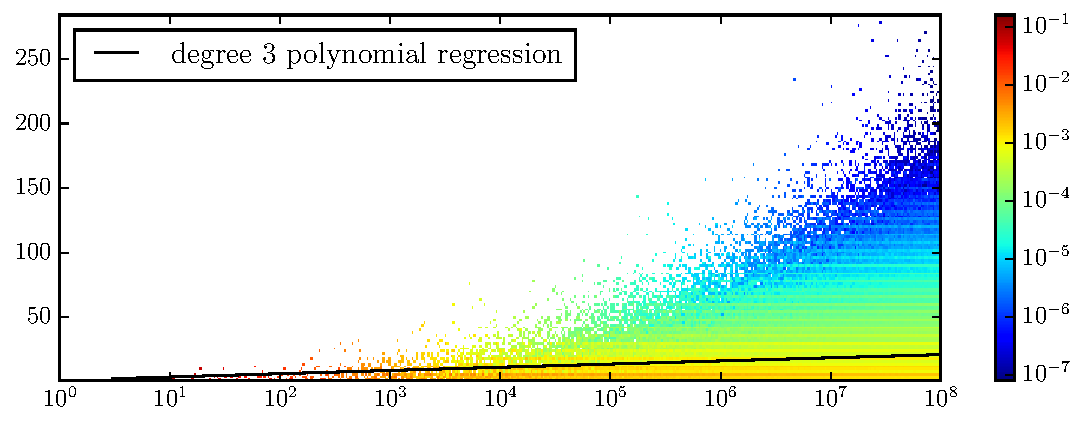
\includegraphics[width=0.85\textwidth]{ffisom/arith_prog}
  \caption{Prime powers $r$ (abscissa) versus smallest integer $u$
    (ordinate) such that $ur+1$ is prime. Abscissa in logarithmic
    scale, density normalized by $\log(x)/x$ and colored in
    logarithmic scale.}
  \label{fig:primes-arith-prog}
\end{figure}

For the cyclotomic algorithm we also require that $\order_\ell(q)$ is
a multiple of $r$. %
Assuming that $q$ is uniformly distributed in $(\Z/\ell\Z)^\times$,
this happens with probability at least $\euler(r)/r\ge 1/2$, hence we
can assume that asymptotically $\ell\in O(r\log(r))$. %

The elliptic algorithm has a similar condition on $\ell$, however it
also requires that the set of curves with trace in $\mathcal{T}$ is
not empty. %
In principle, it is enough to ask that $\ell<4\sqrt{q}$; however, in
order to have a good chance of finding such curves, we set an even
more stringent bound $\ell\in o(\sqrt[4]{q})$. %
Indeed, although it is well known that traces are not evenly
distributed modulo prime numbers~\cite{lenstra87}, it is shown
in~\cite[Th.~1]{castryck+hubrechts13} that the probability that the
trace of a random curve is in $\mathcal{T}$ approaches
$\abs{\mathcal{T}}/\ell\sim r/\ell$, as $\ell$ and $q$ go to infinity,
subject to $\ell\in o(\sqrt[4]{q})$.  %
Thus, also in the elliptic case, we can assume that
$\ell\in O(r\log(r))$.

Finally, we must also take into account the possibility that the
elliptic algorithm fails on the curve output by
Algorithm~\ref{algorithm:selectell}. %
Under the heuristics about the random distribution of elliptic
periods, this possibility only discards one in $O(q^r)$ curves, and is
thus negligible.

The cost of the search for $\ell$ is negligible compared to the cost
of computing the embedding: for each candidate $\ell=ur+1$ we need to
test its primality, and do some computations modulo $\ell$. %
All this is well within $O(\sqrt{r})$ binary operations, using naive
algorithms. %
In the elliptic case we also need to count the number of points of
$O(\log(r))$ elliptic curves defined over $\F_q$, which can be done in
$\tildO\left(\log^5(q)\right)$ binary operations using the
Schoof--Elkies--Atkin algorithm~\cite{schoof95,lercier+sirvent08}. %
This highlights the fact that the elliptic algorithm is only practical
for relatively small $q$.

Summarizing, we can expect heuristically to find a
$\ell\in O(r\log(r))$ that satisfies all the constraints for the
cyclotomic algorithm, leading to an expected running time of
$\tildO(r^{(\omega+1)/2}+\MM(r)\log(q))$ operations in $\F_q$.  %
Similarly, if we assume that $r\log(r)\in o(\sqrt[4]{q})$, we can
expect to find suitable parameters for the elliptic algorithm, leading
to an expected running time of $\tildO(r^2\log(q))$ operations in
$\F_q$, plus $\tildO(\log^5(q))$ binary operations.

Although the complexity of the cyclotomic algorithm looks better, it
must not be neglected that the $\tildO$ notation
hides the cost of taking an auxiliary extension of degree
$O(\log(r))$; whereas the elliptic algorithm, when it applies, does
not incur such overhead. The impact of the hidden terms in the
complexity can be extremely important, as we will show in the next
section. 

The same considerations also apply when comparing Rains' algorithms to
Allombert's. Indeed, the latter performs extremely well when the
degree $s$ of the auxiliary extension is small, but becomes slower as
this degree increases.

In practice, it is hopeless to try and determine the appropriate
bounds for each algorithm from a purely theoretical point of view. The
best approach we can suggest, is to determine parameters at runtime,
and set bounds and thresholds experimentally.
To summarize, given parameters $q$ and $r$, we suggest
the following approach:
\begin{enumerate}
\item If $\gcd(q,r)\ne 1$, run the Artin--Schreier algorithm of
  Section~\ref{sec:fast-artin-schreier}.
\item If $r$ is a power of a small prime $v$, run the algorithm of
  Section~\ref{sec:fast-algor-large}.
\item Determine the order $s$ of $q$ in $(\Z/r\Z)^\times$. If it is
  small enough, run one of the variants of Allombert's algorithm
  presented in Section~\ref{sec:kummer}.
\item Search for suitable parameters for Rains' algorithms. %
  Depending on the best parameters found, run the best option among
  Rains' cyclotomic algorithm, Rains' elliptic algorithm, and
  Allombert's algorithm.
\end{enumerate}

In the next section we shall focus on the last two steps, by comparing
our implementations of the
algorithms involved, thus giving an estimate of the various thresholds
between them.  However we stress that these thresholds are bound to
vary depending on the implementation and the target platform, thus it
is the implementer responsibility to determine them at the moment of
configuring the system.


\section{Experimental Results}
\label{sec:experimental-results}

To validate our results, we implemented the algorithms described in
the previous sections, and compared them to the implementation of
Allombert's algorithm available in PARI/GP 2.8.0~\cite{Pari}, and to
that of Rains' algorithm available in Magma 2.22-7~\cite{MAGMA}. %
The variants of Allombert's algorithm described in
Section~\ref{sec:fast-kummer} were implemented in C on top of the
Flint library, version 2.5.2~\cite{hart2010flint}. %
Rains' cyclotomic and elliptic algorithms were implemented in
SageMath, version 7.5.rc0~\cite{Sage} (which itself uses PARI and
Flint to implement finite fields), with critical code rewritten in
C/Cython. %
Our code is limited to $q$ a prime fitting in a machine-word, and
$m,n$ odd.

We make our code freely available under the open source MIT license,
at \url{https://github.com/defeo/ffisom}. %
Instructions for compiling and running it are available online, as
well as a ready-made cloud environment for testing it, hosted by the
\href{https://mybinder.org/}{Binder} service. %
We stress the fact that our code is experimental and only meant for
research purposes; a subset of the authors is currently working on
integrating part of it in a future release of Flint.

We ran tests for a wide range of primes $q$ between $3$ and
$2^{60}+253$, and prime powers $r$ between $3$ and $2069$. %
% data available at the top of 0x.dat, change it if you change dataset
All tests were run on an Intel(R) Xeon(R) CPU E5-4650 v2 clocked at
2.40GHz. %
We report in Figure~\ref{fig:bench} some statistics, exclusively on
the runs for $100<q<2^{20}$; other ranges show very similar trends. %
The complete datasets, together with more plots and interactive
visualizations are also hosted at
\url{https://github.com/defeo/ffisom}.

\begin{figure}
  \newlength{\mywidth}
  \setlength{\mywidth}{6cm}
  \centering

  \begin{subfigure}{.48\textwidth}
    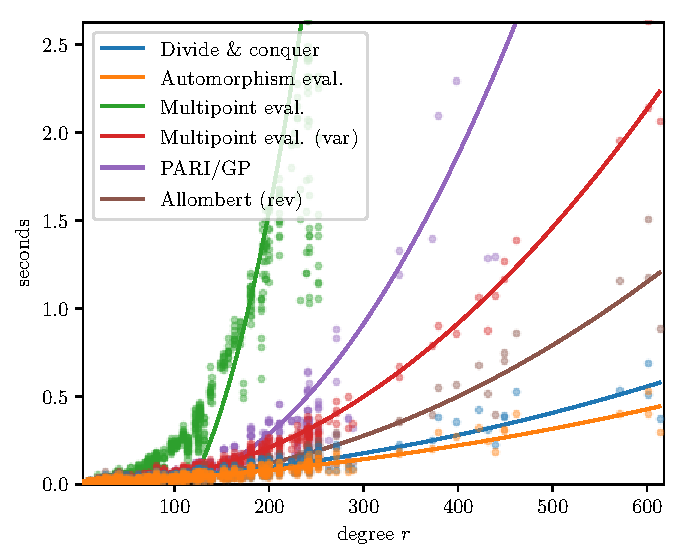
\includegraphics[width=\mywidth]{ffisom/bench-allombert-lowaux}
    \caption{Comparison of various implementations of Allombert's
      algorithm, in the case where the auxiliary degree
      $s=\order_q(r)\le 10$.  Dots represent individual runs, lines
      represent degree 2 linear regressions.}
    \label{fig:bench:allombert-lowaux}
  \end{subfigure}
  \hfill
  \begin{subfigure}{.48\textwidth}
    \noindent
    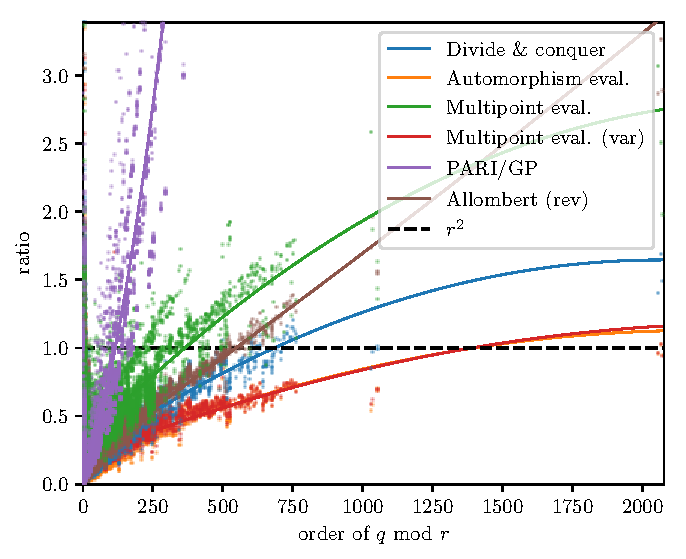
\includegraphics[width=\mywidth]{ffisom/bench-allombert-anyaux}
    \caption{Comparison of various implementations of Allombert's
      algorithm, as a function of the auxiliary degree
      $s=\order_q(r)$.  Individual running times are scaled by down by
      $r^2$.  Dots represent individual runs, lines represent degree 2
      linear regressions.}
    \label{fig:bench:allombert-anyaux}
  \end{subfigure}

  \begin{subfigure}{.48\textwidth}
    \noindent
    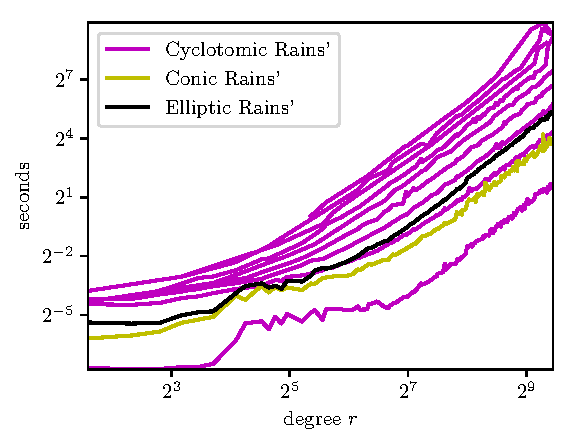
\includegraphics[width=\mywidth]{ffisom/bench-rains}
    \caption{Cyclotomic, conic and elliptic variants of Rains'
      algorithm.  Auxiliary extension degrees $s$ for cyclotomic
      Rains' range between $1$ and $9$. Lines represent median times.}
    \label{fig:bench:rains}
  \end{subfigure}
  \hfill
  \begin{subfigure}{.48\textwidth}
    \noindent
    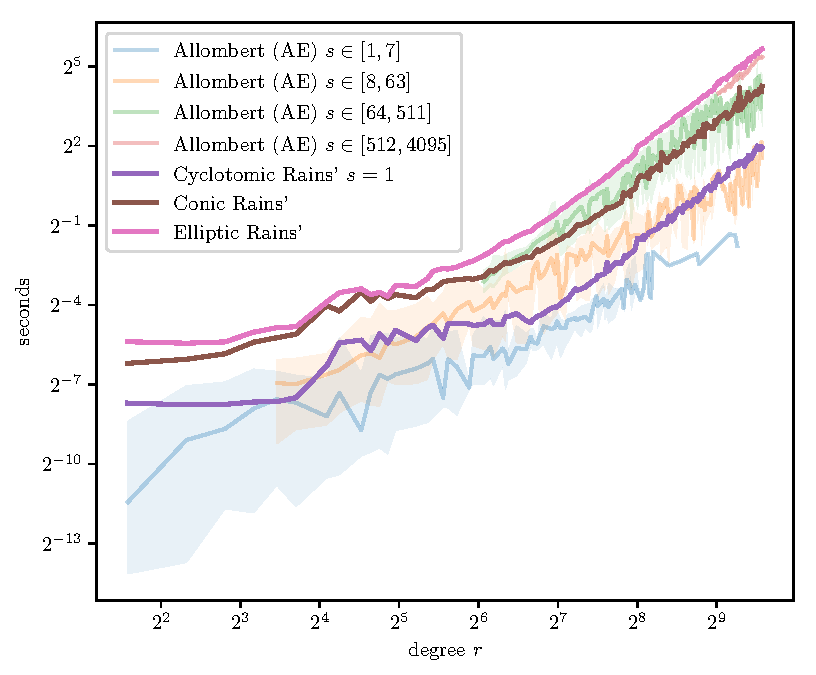
\includegraphics[width=\mywidth]{ffisom/bench-all}
    \caption{Comparison of Allombert's (Automorphism evaluation
      variant) and Rains' algorithms at some fixed auxiliary extension
      degrees $s$. Lines represent median times, shaded areas minimum
      and maximum times.}
    \label{fig:bench:all}
  \end{subfigure}

  \caption{Benchmarks for Rains' and Allombert's algorithms. $q$ is a
    prime between $100$ and $2^{20}$, $r$ is an odd prime power
    varying between $3$ and $2069$.  Plots~\subref{fig:bench:rains}
    and~\subref{fig:bench:all} are in doubly logarithmic scale.}
  \label{fig:bench}
\end{figure}

\begin{figure}
  \centering
  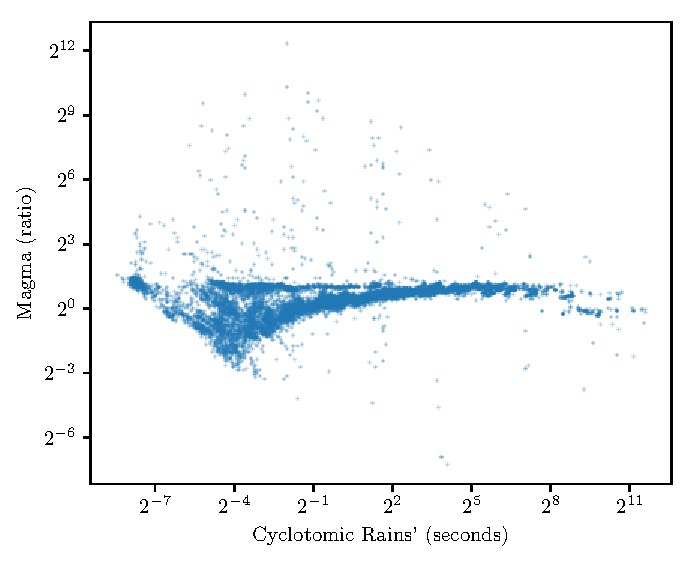
\includegraphics[width=8cm]{ffisom/bench-magma}
  \caption{Comparison of our implementation of Rains' algorithm and
    Magma's. Running time of our implementation in seconds vs ratio of
    Magma running time over ours. Plot in doubly logarithmic scale.}
  \label{fig:bench:magma}
\end{figure}

We start by comparing our implementation of the three variants of
Allombert's algorithm presented in Section~\ref{sec:algor-rely-polyn}
with the original one in PARI. %
In Figure~\ref{fig:bench:allombert-lowaux} we plot running times
against the extension degree $r$, only for cases where the auxiliary
degree $s=\order_q(r)$ is at most $10$: dots represent individual
runs, continuous lines represent degree $2$ linear regressions. %
Analyzing the behavior for arbitrary auxiliary degree $s$ is more
challenging. %
Based on the observation that all variants have essentially quadratic
cost in $r$, in Figure~\ref{fig:bench:allombert-anyaux} we take
running times, we scale them down by $r^2$, and we plot them against
the auxiliary degree $s$. %

The first striking observation is the extremely poor performance of
PARI, especially as $s$ grows. %
To provide a fairer comparison, we re-implemented Allombert's revised
algorithm~\cite{Allombert02-rev}, as faithfully as possible, as
described in Section~\ref{sec:algor-rely-line}; this is the curve
labeled \emph{``Allombert (rev)''} in the graphs. %
For completeness we also implemented the Paterson-Stockmeyer variant
described previously; we do not plot it here, because it overlaps
almost perfectly with our \emph{``Divide \& conquer''} curve. %
Although our re-implementations are considerably faster than PARI, it
is apparent that Allombert's original algorithm does not behave as
well as our new variants.

Focusing now on our three new variants presented in
Section~\ref{sec:algor-rely-polyn}, one can't fail to notice that the
second one, named \emph{``Automorphism evaluation''}, beats the other
two by a great margin, both for small and large auxiliary degree. %
Although the \emph{``Multipoint evaluation''} approach is expected to
eventually beat the other variants as $s$ grows, the cross point seems
to be extremely far from the parameters we explored. %
However, we notice that the naive variant of \emph{``Multipoint
  evaluation''} not using the iterated Frobenius technique (labeled
\emph{``Multipoint evaluation (var)''} in the graphs), starts poorly,
then quickly catches \emph{``Automorphism evaluation''} as $s$ grows.

Finally, comparing the variants as $q$ grows shows\footnote{For lack
  of space we do not show these graphs here, but see
  \url{https://github.com/defeo/ffisom/blob/master/notebooks/benchmarks.ipynb}.}
that the hierarchy between them is essentially unchanged as $q$
approaches $2^{64}$. %
We could not test larger values of $q$, as our code is limited to
machine-word size.

Now we shift to Rains' algorithm and its variants. %
In comparing our implementation with Magma's, discarding outliers, we
obtain a fairly consistent speed-up of about 30\% (see
Figure~\ref{fig:bench:magma}); hence we will compare these algorithms
only based on our timings. %
In Figure~\ref{fig:bench:rains} we group runs of the cyclotomic
algorithm by the degree $s$ of the auxiliary extension, and we plot
median times against the degree $r$; only the graphs for $s<10$ are
shown in the figure. %
We observe a very large gap between $s=1$ and larger $s$ ($s=2$ is
$8-16$ times slower). This is partly due to the fact that we use
generic Python code to construct auxiliary extensions, rather than
dedicated C; however, a large gap is unavoidable, due to the added
cost of computing in extension fields. %
We also plot median times for the elliptic variant and for the conic
variant (see Appendix~\ref{app:rains-vars}). %
It is apparent that the elliptic algorithm outperforms the cyclotomic
one as soon as $s\ge 3$, and that the conic algorithm conveniently
replaces the case $s=2$. %
Thus, at least for the parameter ranges we have tested, the cyclotomic
algorithm with auxiliary extensions seems of limited interest. %
Plotting against the prime $q$ instead of the degree $r$ shows
essentially the same behavior\footnote{Again, see
  \url{https://github.com/defeo/ffisom/blob/master/notebooks/benchmarks.ipynb}
  for a plot.}, however it should be reminded that the elliptic
variant becomes very poor when $q$ grows larger than a machine-word,
because of the cost of point counting.

Finally, in Figure~\ref{fig:bench:all} we compare Rains' algorithms
against Allombert's. %
In light of the excellent performances of the \emph{``Automorphism
  evaluation''} variant of Allombert's algorithm, we only plot the
performances for this variant. %
We plot, against the degree $r$, runs of Allombert's algorithm grouped
by ranges of the auxiliary degree $\order_r(q)$: we shade the area
between minimum and maximum running times, and trace the median
time. %
We also take from Figure~\ref{fig:bench:rains} the graphs for the
cyclotomic (only $s=1$), the conic and the elliptic variants of Rains'
algorithm. %
We notice that Allombert's algorithm, even with relatively large
auxiliary degrees, is extremely fast; the cyclotomic algorithm only
beats it when $\order_r(q)$ goes beyond 10 to 50, the conic algorithm
only beats extremely large $\order_r(q)$, and the elliptic algorithm
is never better. %
We also observe that Allombert's algorithm has a better asymptotic
behavior as the degree $r$ grows.

In light of these comparisons, it seems that the absolute winner is
our \emph{Automorphism evaluation} variant of Allombert's algorithm,
with Rains' cyclotomic algorithm being only occasionally more
interesting. %
Obviously, the comparisons are only relevant to our own code and test
conditions. Other implementations and benchmarks will likely find
slightly different cross-points for the algorithms.

%%%%%%%%%%%%%%%%%%%%%%%%%%%%%%%%%%
%%%%%%%%%%%%%%%%%%%%%%%%%%%%%%%%%%

%\appendix

%%%%%%%%%%%%%%%%%%%%%%%%%%%%%%%%%%

\section{Rain's conic algorithm}
\label{app:rains-vars}

We have seen that Rains' cyclotomic algorithm suffers in practice from
the need to build a field extension $k'$ of $k$. %
The conic variant we are going to present reduces the degree of the
field extension from $s=[k':k]$ to $s/2$ whenever $s$ is even. %
This is especially useful when $s=2$, as highlighted in
Section~\ref{sec:experimental-results}. %
The algorithm is similar in spirit to Williams' $p+1$ factoring
method~\cite{williams1982}, where the arithmetic of the norm $1$
subgroup of ${k'}^*$ is performed using Lucas sequences on a subfield
of index $2$ of $k'$.

Let $\F$ be a finite field of odd characteristic, let $\Delta\in\F$ be
a quadratic non-residue, let $\delta$ be an element of the algebraic
closure of $\F$ such that $\delta^2=\Delta$, and define the norm $1$
subgroup of $\F[\delta]^*$ as
\[T_2(\F) = \{(x+\delta y)/2 \;\mid\; x,y\in\F \text{ and } x^2-\Delta
  y^2 = 4\};\] %
it is easy to verify that $T_2(\F)$ forms a group under
multiplication. %
If we see the elements $(x+\delta y)/2$ as points $(x,y)$ on a conic
$x^2-\Delta y^2=4$, the group law of $T_2(\F)$ induces a group law on
the conic. %
By projecting onto the $x$-coordinate, a straightforward calculation
shows that, for any point $(\theta,*)$ on the conic, its $n$-th power
has coordinates $(\theta_n,*)$, where $\theta_n$ is defined by the
Lucas sequence
\[\theta_0 = 2, \quad \theta_1 = \theta, \quad \theta_{i+1}=\theta\theta_i-\theta_{i-1}.\] %
We shall denote by $[n]$ the map $\theta\mapsto\theta_n$; notice how
it does not depend on the choice of $\Delta$.

The generalization of Rains' algorithm is now obvious: by projecting
on the $x$-coordinate, we work in a field extension twice as small
compared to the original algorithm. %
This is summarized in Algorithm~\ref{algorithm:rains-conic}.

\begin{algorithm}
    \caption{Rains' conic algorithm}
  \label{algorithm:rains-conic}
  \begin{algorithmic}[1]
    \REQUIRE A field extension $k/\F_q$ of degree $r$; a prime $\ell$
    such that
    \begin{itemize}
    \item $(\Z/\ell\Z)^\times = \langle q\rangle \times S$ for some $S$,
    \item $\#\langle q\rangle = 2rs$ for some integer $s$;
    \end{itemize}
    a polynomial $h$ of degree $s$ irreducible over $k$.
    \ENSURE A normal generator of $k$ over $\F_q$,
    with a uniquely defined Galois orbit.
    
    \STATE Construct the field extension $k'=k[Z]/h(Z)$;
    \REPEAT
    \REPEAT
    \STATE Take a random element $\theta\in k'$,
    \UNTIL\label{algorithm:rains-conic:sqtest} $\theta^2-4$ is a quadratic non-residue;
    \STATE\label{algorithm:rains-conic:power} Compute $\zeta=[(\#k'+1)/\ell]\theta$,
    \UNTIL $\zeta\ne2$;
    \STATE\label{algorithm:rains-conic:period} Compute $\eta(\zeta) \leftarrow \sum_{\sigma\in S}[\sigma]\zeta$;
    \RETURN\label{algorithm:rains-conic:trace} $\alpha \leftarrow \trace_{k'/k}\eta(\zeta) = \sum_{i=0}^{s-1}[q^{ri}]\eta(\zeta)$.
  \end{algorithmic}
\end{algorithm}

\begin{proposition}
  Algorithm~\ref{algorithm:rains-conic} is correct: on input
  $q,r,\ell,s$ it returns an element in the same Galois orbit as
  Algorithm~\ref{algorithm:rains-cyclo} on input $q,r,\ell,2s$. %
  It computes its output using $O(\MM(sr)(sr\log(q)+(\ell/r)\log(\ell)))$
  operations in $\F_q$ on average, or $\tildO((sr)^2\log(q))$ assuming
  $\ell\in o(sr^2)$.
\end{proposition}
\begin{proof}
  By construction, all the $\ell$-th roots of unity are in
  $T_2(k')$. %
  Observe that if $(x+\delta y)/2$ is in $T_2(k')$, then its trace
  over $k'$ is equal to $x$. %
  Hence, the value $\zeta$ computed in
  Step~\ref{algorithm:rains-conic:power} is the trace over $k'$ of a
  primitive $\ell$-th root of unity. %
  We conclude by comparing this algorithm with
  Algorithm~\ref{algorithm:rains-cyclo}.

  The non-residuosity test in Step~\ref{algorithm:rains-conic:sqtest}
  is done by verifying that the $(\#k'-1)/2$-th power of $\theta$ is
  equal to $-1$. %
  We do this in $O(sr\log(q))$ operations in $k'$, or
  $O(sr\MM(sr)\log(q))$ operations in $\F_q$.

  To implement the other steps, we need to evaluate the map $[n]$
  efficiently. %
  We have the following classical relationships for the Lucas sequence
  of $\theta$:
  \begin{equation*}
    \theta_{2i} = \theta_{i}^2-2,\quad
    \theta_{2i+1} = \theta_i\theta_{i+1} - \theta,\quad
    \theta_{2i+2} = \theta_{i+1}^2-2.
  \end{equation*}
  Starting with $\theta_0=2$ and $\theta_1=\theta$, we use a binary
  scheme to deduce $\theta_i,\theta_{i+1}$ from
  $\theta_{\lfloor i/2\rfloor},\theta_{\lfloor i/2\rfloor+1}$. %
  We reach $\theta_n$ after $O(\log(n))$ steps, each requiring a
  constant number of operations in $k'$.

  Hence, Step~\ref{algorithm:rains-conic:power} costs
  $O(sr\MM(sr)\log(q))$ operations in $\F_q$, while
  Steps~\ref{algorithm:rains-conic:period}
  and~\ref{algorithm:rains-conic:trace} together cost
  $O((\MM(sr)(\ell/r)\log(\ell))$.
\end{proof}

Although this variant does not exploit the asymptotic improvement
offered by Proposition~\ref{prop:trace-like}, the fact that its
auxiliary degree $s$ is half the one of the original algorithm usually
gives an interesting practical improvement. %
Step~\ref{algorithm:rains-conic:power} can be modified so as to avoid
the premature projection on the $x$-axis, so that the algorithms of
Proposition~\ref{prop:trace-like} apply. %
We leave the details of this variant to the reader.


%%%%%%%%%%%%%%%%%%%%%%%%%%%%%%%%%%

%%%%%%%%%%%%%%%%%%%%%%%%%%%%%%%%%%
%%%%%%%%%%%%%%%%%%%%%%%%%%%%%%%%%%



% Local Variables:
% ispell-local-dictionary:"american"
% End:

%  LocalWords:  isomorphism cyclotomic coprime subfield Frobenius
%  LocalWords:  endomorphism eigenspace Allombert's polynomially
%  LocalWords:  automorphism morphism morphisms
}
{\newcommand{\dottriangle}[2][\i-\j]{  \foreach \i in {0,...,#2} {    \foreach \j in {0,...,\i} {      \draw(\i,\j) node{#1};    }  }}


\let\prop\proposition
\let\endprop\endproposition

\newcommand{\QQ}{{\mathbb{Q}}}
\newcommand{\ZZ}{{\mathbb{Z}}}
\newcommand{\RR}{{\mathbb{R}}}
\newcommand{\FF}{{\mathbb{F}}}
\newcommand{\VV}{{\mathcal{V}}}
\newcommand{\EE}{{\mathcal{E}}}
\newcommand{\iso}{\cong}
\newcommand{\id}{\operatorname{sID}}
\newcommand{\cyc}[1]{{\langle #1 \rangle}}
\def\abs#1{\left|#1\right|}


\chapter{Towards quantum-resistant cryptosystems from supersingular elliptic
curve isogenies}

\begin{abstract}
We present new candidates for quantum-resistant public-key
cryptosystems based on the conjectured difficulty of finding isogenies
between supersingular elliptic curves.  The main technical idea in our
scheme is that we transmit the images of torsion bases under the isogeny
in order to allow the parties to construct a shared commutative square
despite the noncommutativity of the endomorphism ring.
We give a precise formulation of the necessary computational assumptions
along with a discussion of their validity, and prove the
security of our
protocols under these assumptions. In addition, we present implementation
results showing that our protocols are multiple orders of magnitude faster
than previous isogeny-based cryptosystems over ordinary curves.

This paper is an extended version of~\cite{jao+defeo2011}. We add a new
zero-knowledge identification scheme, and detailed security proofs for
the protocols. We also present a new, asymptotically faster, algorithm
for key generation, a thorough study of its optimization, and new
experimental data.
\end{abstract}

{\small This article was authored with David Jao and Jérôme Plût. It
  originally appeared in the \textit{Journal of Mathematical
    Cryptology}, 8.3 (2014), \doi{10.1515/jmc-2012-0015}.}

%%%%%%%%%%%%%%%%%%%%%%%%%%%%%%%%%%

\section{Introduction}

The Diffie-Hellman scheme is a fundamental protocol for public-key
exchange between two parties. Its original definition over finite
fields is based on the hardness of computing the map $g,g^a,g^b
\mapsto g^{ab}$ for $g \in \FF_p^*$. Recently, Stolbunov~\cite{Stol}
proposed a Diffie-Hellman type system based on the difficulty of
computing isogenies between ordinary elliptic curves, with the stated
aim of obtaining quantum-resistant cryptographic protocols.  The
fastest known (classical) probabilistic algorithm for solving this
problem is the algorithm of Galbraith and Stolbunov~\cite{galbraith+stolbunov11}, based
on the algorithm of Galbraith, Hess, and Smart~\cite{GHS}. This
algorithm is exponential, with a worst-case running time of
$O(\sqrt[4]{q})$. However, on a quantum computer, recent work of
Childs et al.~\cite{childs2014constructing} showed that the private keys in
Stolbunov's system can be recovered in subexponential time. Moreover,
even if we only use classical attacks in assessing security levels,
Stolbunov's scheme requires 229 seconds (even with precomputation) to
perform one key exchange operation at the 128-bit security level on a
desktop PC~\cite[Table 1]{Stol}.

In this work we present isogeny-based key-exchange, encryption, and
identification schemes that address both the performance and security
drawbacks of Stolbunov's system. Our primitive achieves performance on
the order of 60 milliseconds (cf. Section~\ref{sidh:sec:imp}) at the
128-bit security level (as measured against the fastest known quantum
attacks) using desktop PCs, making our schemes far faster than
Stolbunov's. In terms of security, our schemes are not vulnerable to
the algorithm of Childs et al.~\cite{childs2014constructing}, nor to any algorithm of
this type, since they are not based on a group action. The fastest
known attacks against our schemes, even on quantum computers, require
fully exponential time. Our schemes involve new computational
assumptions upon which their quantum resistance is based, and like all
new computational assumptions, further study and the passage of time
is needed for validation. Nevertheless, we believe our proposal
represents a promising candidate for quantum-resistant isogeny-based
public-key cryptography.

Our proposal, presented in Section~\ref{sidh:sec:kep}, uses isogenies
between \emph{supersingular} elliptic curves rather than ordinary
elliptic curves. The main technical difficulty is that, in the
supersingular case, the endomorphism ring is noncommutative, whereas
Diffie-Hellman type protocols require commutativity. We show how to
overcome this obstacle by providing the outputs of the isogeny on
certain points as auxiliary input to the protocols. To the best of our
knowledge, nothing similar to this idea has ever previously appeared
in the literature. Providing this auxiliary input does not seem to
make the problem of finding isogenies any easier, and the added
difficulty arising from noncommutativity seems to make our protocols
stronger; see Section~\ref{sidh:subsec:hardness} for a full discussion. The
multiple orders of magnitude of performance gains in our scheme arise
from the fact that supersingular isogeny graphs are much faster to
navigate than ordinary graphs, as described in
Section~\ref{sidh:sec:alg}. In Sections~\ref{sidh:sec:security}
and~\ref{sidh:sec:proof} we provide formal statements of the hardness
assumptions and security reductions for our system. Finally, in
Section~\ref{sidh:sec:imp} we present implementation results confirming the
correctness and performance of our protocol.


\section{Isogenies}\label{sidh:isogenies}
Let $E_1$ and $E_2$ be elliptic curves defined over a finite field
$\FF_q$.
An isogeny $\phi: E_1 \rightarrow E_2$ defined over $\FF_q$ is a
non-constant rational map defined over $\FF_q$ which is also a group
homomorphism from $E_1(\FF_q)$ to $E_2(\FF_q)$ \cite[III.4]{Sil}. The
degree of an isogeny is its degree as a rational map.  For separable
isogenies, having degree $\ell$ implies that the kernel of the
isogeny has cardinality $\ell$.
Every isogeny of degree greater than 1 can be factored into a
composition of isogenies of prime degree over $\bar{\FF}_q$
\cite{cryptoeprint:2006:291}.

An endomorphism of an elliptic curve $E$ defined over $\FF_q$ is an
isogeny $E \rightarrow E$ defined over $\FF_{q^m}$ for some $m$. The
set of endomorphisms of $E$ together with the zero map forms a ring
under the operations of pointwise addition and composition; this ring
is called the endomorphism ring of $E$ and denoted $\End(E)$. The ring
$\End(E)$ is isomorphic either to an order in a quaternion algebra or
to an order in an imaginary quadratic field \cite[V.3.1]{Sil}; in the
first case we say $E$ is supersingular and in the second case we say
$E$ is ordinary.

Two elliptic curves $E_1$ and $E_2$ defined over $\FF_q$ are said to
be isogenous over $\FF_q$ if there exists an isogeny $\phi\colon E_1
\to E_2$ defined over $\FF_q$. A theorem of Tate states that
two curves $E_1$ and $E_2$ are isogenous over $\FF_q$ if and only if
$\#E_1(\FF_q) = \#E_2(\FF_q)$ \cite[$\S$3]{Tate}. Since every isogeny
has a dual isogeny \cite[III.6.1]{Sil}, the property of being
isogenous over $\FF_q$ is an equivalence relation on the finite set of
$\bar{\FF}_q$-isomorphism classes of elliptic curves defined over
$\FF_q$.  Accordingly, we define an isogeny class to be an equivalence
class of elliptic curves, taken up to $\bar{\FF}_q$-isomorphism, under
this equivalence relation.

The $\ell$-torsion group of $E$, denoted $E[\ell]$, is the set of all
points $P \in E(\bar{\FF}_q)$ such that $\ell P$ is the identity. For
$\ell$ such that $p\nmid \ell$, we have $E[\ell] \cong \ZZ/\ell\ZZ \oplus
\ZZ/\ell\ZZ.$

Curves in the same isogeny class are either all supersingular or all
ordinary. 
We assume for the remainder of this paper that
we are in the supersingular case. Because we only care about curves
up to isomorphism, and every supersingular curve is
isomorphic to a curve defined over the field~$\FF_{p^2}$, we limit
ourselves to this base field.

For every
prime $\ell \nmid p$, there exist exactly $\ell+1$ isogenies (counting
multiplicities) of degree $\ell$ originating from any given such
supersingular curve.
Given an elliptic curve $E$ and a finite subgroup $\Phi$ of $E$, there
is up to isomorphism a unique isogeny $E \to E'$ having kernel
$\Phi$~\cite[III.4.12]{Sil}. Hence we can identify an isogeny by
specifying its kernel, and conversely given a kernel subgroup the
corresponding isogeny can be computed using V\'elu's
formulas~\cite{velu71}. Typically, this correspondence is of little use,
since the kernel, or any representation thereof, is usually as
unwieldy as the isogeny itself. However, in the special case of
kernels generated by $\FF_{p^2}$-rational points of smooth order,
specifying a generator of the kernel allows for compact representation
and efficient computation of the corresponding isogeny, as we
demonstrate in Section~\ref{sidh:sec:alg}.


\subsection{Ramanujan graphs}\label{sidh:ram_graph} 

Let $G = (\mathcal{V},\EE)$ be a finite graph on $h$ vertices $\VV$
with undirected edges $\EE$.  Suppose $G$ is a regular graph of degree
$k$, i.e., exactly $k$ edges meet at each vertex. Given a
labeling of the vertices $\VV = \{v_1,\ldots , v_h\}$, the adjacency
matrix of $G$ is the symmetric $h\times h$ matrix $A$ whose $ij$-th
entry $A_{i,j} = 1$ if an edge exists between $v_i$ and $v_j$ and 0
otherwise.

It is convenient to identify functions on $\VV$ with vectors in
$\RR^h$ via this labeling, and therefore also think of $A$ as a
self-adjoint operator on $L^2(\VV)$.  All of the eigenvalues of $A$
satisfy the bound $|\lambda| \leq k$. Constant vectors are
eigenfunctions of $A$ with eigenvalue $k$, which for obvious reasons
is called the trivial eigenvalue $\lambda_{\operatorname{triv}}$. A
family of such graphs $G$ with $h \rightarrow \infty$ is said to be a
sequence of \emph{expander graphs} if all other eigenvalues of their
adjacency matrices are bounded away from
$\lambda_{\operatorname{triv}}= k$ by a fixed
amount.\footnote{Expansion is usually phrased in terms of the number
  of neighbors of subsets of $G$, but the spectral condition here is
  equivalent for $k$-regular graphs and also more useful for our
  purposes.}  In particular, no other eigenvalue is equal to $k$; this
implies the graph is connected.  A Ramanujan graph is a special type
of expander which has $|\lambda| \leq 2\sqrt{k-1}$ for any nontrivial
eigenvalue which is not equal to $-k$ (this last possibility happens
if and only if the graph is bipartite). The Ramanujan property was
first defined in \cite{LubPS}. It characterizes the optimal separation
between the two largest eigenvalues of the graph adjacency matrix, and
implies the expansion property.

A fundamental use of expanders is to prove the rapid mixing of the
random walk on $\VV$ along the edges $\EE$. The following rapid mixing
result is standard but we present it below for completeness. For the
proof, see~\cite{jao+miller+venkatesan09} or \cite{DSV,Lub,Sarnak}.

\begin{prop}\label{sidh:prop:mixing} Let $G$ be a regular graph of degree
  $k$ on $h$ vertices. Suppose that the eigenvalue $\lambda$ of any
  nonconstant eigenvector satisfies the bound $|\lambda| \leq c$ for
  some $c < k$. Let $S$ be any subset of the vertices of $G$, and $x$
  be any vertex in $G$. Then a random walk of length at least
  $\frac{\log 2h/|S|^{1/2}}{\log k/c}$ starting from $x$ will land in
  $S$ with probability at least $\frac{|S|}{2h} = \frac{|S|}{2|G|}$.
\end{prop}

\subsection{Isogeny graphs}\label{sidh:isog_graph} 

An isogeny graph is a graph whose nodes consist of all elliptic curves
in $\FF_q$ belonging to a fixed isogeny class, up to
$\bar{\FF}_q$-isomorphism (so that two elliptic curves which are
isomorphic over $\bar{\FF}_q$ represent the same node in the
graph). In practice, the nodes are represented using $j$-invariants,
which are invariant up to isomorphism. 
Isogeny graphs for supersingular elliptic curves were first considered
by Mestre \cite{mestre86}, and were shown by Pizer \cite{pizer1,pizer2}
to have the Ramanujan property.

Every supersingular elliptic curve in characteristic $p$ is defined
over either $\FF_p$ or $\FF_{p^2}$ \cite{Sil}, so it suffices to fix
$\FF_q = \FF_{p^2}$ as the field of definition for this
discussion. Thus, in contrast to ordinary curves, there are a finite
number of isomorphism classes of supersingular curves in any given isogeny class;
this number is in fact $g+1$, where $g$ is the genus of the modular curve $X_0(p)$,
which is roughly $p/12$. It turns out that all supersingular
curves defined over $\FF_{p^2}$ belong to the same isogeny
class~\cite{mestre86}. For a fixed prime value of $\ell \neq p$, we
define the vertices of the supersingular isogeny graph $\mathcal{G}$
to consist of these $g$ isomorphism classes of curves, with
edges given by isomorphism classes of degree-$\ell$ isogenies,
defined as follows: two isogenies $\phi_1, \phi_2 \colon E_i \to E_j$
are isomorphic if there exists an automorphism $\alpha \in
\text{Aut}(E_j)$ (i.e., an invertible endomorphism) such that $\phi_2
= \alpha\phi_1$. Pizer~\cite{pizer1,pizer2} has shown that
$\mathcal{G}$ is a connected $k = \ell + 1$-regular multigraph
satisfying the Ramanujan bound of $|\lambda| \leq 2\sqrt{\ell} =
2\sqrt{k - 1}$ for the nontrivial eigenvalues of its adjacency matrix.


\section{Public-key cryptosystems based on supersingular curves}\label{sidh:sec:kep}

In this section we present a key-exchange protocol and a public-key
cryptosystem analogous to those of \cite{rostovtsev+stolbunov06,Stol}, and a
zero-knowledge identification scheme, all using supersingular elliptic
curves.

Our protocols require supersingular curves of smooth order. Such
curves are normally unsuitable for cryptography since discrete
logarithms on them are easy. However, since the discrete logarithm
problem is unimportant in our setting, this issue does not affect
us. In the supersingular setting, it is easy to construct curves of
smooth order, and using a smooth order curve will give a large number
of isogenies that are fast to compute. Specifically, we fix $\FF_q =
\FF_{p^2}$ as the field of definition, where $p$ is a prime of the
form $\ell_A^{e_A} \ell_B^{e_B}\cdot f \pm 1$.  Here $\ell_A$ and
$\ell_B$ are small primes, and $f$ is a cofactor such that $p$ is
prime.  Then we construct a supersingular curve $E$ defined over
$\FF_q$ of cardinality $(\ell_A^{e_A}\ell_B^{e_B}f)^2$. By
construction, $E[\ell_A^{e_A}]$ is $\FF_q$-rational and contains
$\ell_A^{e_A-1}(\ell_A+1)$ cyclic subgroups of order $\ell_A^{e_A}$,
each defining a different isogeny; the analogous statement holds for
$E[\ell_B^{e_B}]$.

Our protocols revolve around the following commutative diagram
\begin{equation}
  \label{sidh:eq:square}
  \begin{tikzpicture}[xscale=2,yscale=1.5,baseline=(current bounding box.east)]
    \node(0) at (0,0) {$E$};
    \node(S) at (1,0) {$E/\cyc{P}$};
    \node(R) at (0,-1) {$E/\cyc{Q}$};
    \node(SR) at (1,-1) {$E/\cyc{P,Q}$};
    \path[->] (0) edge node[auto] {$\phi$} (S);
    \path[->] (0) edge node[auto,swap] {$\psi$} (R);
    \path[->] (S) edge (SR);
    \path[->] (R) edge (SR);
  \end{tikzpicture}
\end{equation}
where $\phi$ and $\psi$ are random walks in the graphs of isogenies of
degrees $\ell_A$ and $\ell_B$ respectively. Their security is based on
the difficulty of finding a path connecting two given vertices in a
graph of supersingular isogenies. We refer to Section~\ref{sidh:sec:alg}
for low-level algorithmic details, and Section~\ref{sidh:sec:security} for
a full discussion of security.

\subsection{Zero-knowledge proof of identity}\label{sidh:subsec:zk}

We begin with the protocol which is easiest to understand. Peggy
knows a cyclic degree $\ell_A^{e_A}$ isogeny $\phi:E \to E/\cyc{S}$,
with the curves $E$ and $E/\cyc{S}$ publicly known, and wants to prove to
Vic that she knows a generator for $\cyc{S}$, without revealing it.

Our protocol is loosely inspired by the zero-knowledge proof of
membership for Graph
Isomorphism~\cite{goldreich+micali+widgerson91}. In that protocol,
Peggy shows that she knows a graph isomorphism $G \simeq G'$ by first
publishing a random $H$ such that the following diagram commutes
\begin{equation}
  \label{sidh:eq:gi}
  \begin{tikzpicture}[xscale=1.5,yscale=1.5,baseline=(current bounding box.east)]
    \node(G) at (0,0) {$G$};
    \node(G') at (1,0) {$G'$};
    \node(H) at (0.5,-1) {$H$};
    \path[<->] (G) edge (G');
    \path[<->] (G) edge node[auto,swap] {$\phi$} (H);
    \path[<->] (G') edge node[auto] {$\psi$} (H);
  \end{tikzpicture}  
\end{equation}
and then revealing only one among $\phi$ and $\psi$. Intuitively, this
protocol is \emph{perfectly} zero-knowledge because the information
that Peggy reveals (i.e., a random permutation of $G$ or $G'$) could
be easily computed by anyone without her help.

In an analogous way, our protocol consists in publishing the vertices
of diagram~\eqref{sidh:eq:square}, and then revealing some, but not all, of
its arrows. Unlike the case of Graph Isomorphism, in our protocol
Peggy needs to use her secret knowledge to create the diagram, thus we
cannot achieve a \emph{perfect} zero-knowledge. Nevertheless, we will
show in Section~\ref{sidh:sec:proof} that, under suitable assumptions, our
protocol is \emph{computationally} zero-knowledge.

We show below the diagram used in our protocol. $\cyc{S}$ is the
kernel of the secret isogeny $\phi$ of degree $\ell_A^{e_A}$, while
$\cyc{R}$ is a cyclic group of order $\ell_B^{e_B}$.
\begin{equation}
  \label{sidh:eq:zk}
  \begin{tikzpicture}[xscale=2,yscale=1.5,baseline=(current bounding box.east)]
    \node(0) at (0,0) {$E$};
    \node(S) at (1,0) {$E/\cyc{S}$};
    \node(R) at (0,-1) {$E/\cyc{R}$};
    \node(SR) at (1,-1) {$E/\cyc{S,R}$};
    \path[->] (0) edge node[auto] {$\phi$} (S);
    \path[->] (0) edge node[auto,swap] {$\psi$} (R);
    \path[->] (S) edge node[auto] {$\psi'$} (SR);
    \path[->] (R) edge node[auto] {$\phi'$} (SR);
  \end{tikzpicture}
\end{equation}

Peggy can compute the diagram as follows:
\begin{itemize}
\item She uses V\'elu's formulas to compute the isogeny $\psi:E\to
  E/\cyc{R}$;
\item She computes $R' = \phi(R)$ and the isogeny $\psi':E/\cyc{S}\to
  E/\cyc{S,R}$;
\item She computes $S' = \psi(S)$ and the isogeny
  $\phi':E/\cyc{R}\to E/\cyc{S,R}$.
\end{itemize}

Now, the natural question is: which arrows of the diagram can Peggy
reveal without compromising her secret $\phi$? It is not hard to see,
and we will show it in Theorem~\ref{sidh:thm:zk-proof}, that the knowledge
of $(\psi,\phi')$ or $(\psi',\phi')$ allows anyone to compute the
kernel of $\phi$. However, we will argue that there is no obvious way
to compute $\phi$ from the sole knowledge of $\phi'$. Revealing one of
$\psi$ or $\psi'$ is no problem either, however revealing
$(\psi,\psi')$ altogether is more subtle. Indeed, revealing the points
$R$ and $\phi(R)$ uncovers some information on the action of $\phi$ on
$E[\ell_B^{e_B}]$: it is to be expected that after a few iterations
Peggy will reveal a basis $(P,Q)$ of $E[\ell_B^{e_B}]$ and the
respective images $\phi(P)$, $\phi(Q)$, thus allowing anyone to
evaluate $\phi$ on the whole $E[\ell_B^{e_B}]$. Nevertheless, we
conjecture that this leakage does not compromise Peggy's secret
either, and we make these data part of the public
parameters.\footnote{An alternative solution, that intuitively leaks
  less information on $\phi$, would be to publish random generators of
  $\cyc{R}$ and $\cyc{\phi(R)}$.  However, it is not clear that this
  idea would considerably improve the security of the protocol, and we
  will not pursue it further for coherence with the protocols that
  will follow.}

Finally, we present our protocol.

\begin{description}
\item[Secret parameters] A supersingular curve $E$ defined over
  $\FF_q$ and a primitive $\ell_A^{e_A}$-torsion point $S$ defining an
  isogeny $\phi:E\to E/\cyc{S}$.
\item[Public parameters] The curves $E$ and $E/\cyc{S}$. Generators
  $P,Q$ of $E[\ell_B^{e_B}]$ and their images $\phi(P),\phi(Q)$.
\item[Identification] Repeat $m$ times:
  \begin{enumerate}
  \item Peggy chooses a random primitive $\ell_B^{e_B}$-torsion point
    $R$ and computes diagram~\eqref{sidh:eq:zk}.
  \item Peggy sends the curves $E_1=E/\cyc{R}$ and $E_2=E/\cyc{S,R}$ to Vic.
  \item Vic selects a random bit $b$ and sends it to Peggy.
  \item If $b=0$, Peggy reveals the points $R$ and $\phi(R')$. Vic
    accepts if they have order $\ell_b^{e_B}$ and generate the kernels
    of isogenies $E\to E_1$ and $E/\cyc{S}\to E_2$, respectively.
  \item If $b=1$, Peggy reveals the point $\psi(S)$. Vic accepts if it
    has order $\ell_A^{e_A}$ and generates the kernel of an isogeny
    $E_1\to E_2$.
  \end{enumerate}
\end{description}


\subsection{Key exchange}\label{sidh:subsec:kep}

The key exchange protocol is a variation \emph{\`a la} Diffie-Hellman
over diagram~\eqref{sidh:eq:square}. The idea is to let Alice choose
$\phi$, while Bob chooses $\psi$. Although similar in spirit to the
protocol based on the action of the class group on ordinary elliptic
curves of~\cite{Stol}, a main technical difference is that, since
ideal classes no longer commute (or indeed even multiply together) in
the supersingular case, extra information must be communicated as part
of the protocol in order to ensure that both parties arrive at the
same common value.

\begin{figure}[t]
\begin{center} 
\begin{tabular}{l c l}
\cline{1-1} \cline{3-3} 
$\mathcal{A}$ & & $\mathcal{B}$ \\ 
\cline{1-1} \cline{3-3} 
\textbf{Input:} $A,B,\id$ & & \textbf{Input:} $B$ \\
$m_A,n_A \in_{R} \ZZ/\ell_A^{e_A}\ZZ$ & & $m_B,n_B \in_{R} \ZZ/\ell_B^{e_B}\ZZ$ \\
$\phi_A := E_0/\scriptstyle{\cyc{[m_A]P_A+[n_A]Q_A}}$ & & $\phi_B :=
E_0/\scriptstyle{\cyc{[m_B]P_B+[n_B]Q_B}}$ \\ 
 & $\xrightarrow[]{\substack{A, \id \\ \phi_A(P_B),\\ \phi_A(Q_B),\\ E_A}} $ &  \\
  & $\xleftarrow[]{\substack{B, \id \\ \phi_B(P_A),\\ \phi_B(Q_A),\\ E_B}} $ &  \\
$E_{AB} := $ &  & $ E_{BA} := $ \\
$E_B/\scriptstyle{\cyc{[m_A]\phi_B(P_A)+[n_A]\phi_B(Q_A)}} $ &  & $
E_A/\scriptstyle{\cyc{[m_B]\phi_A(P_B)+[n_B]\phi_A(Q_B)}}$ \\
\textbf{Output:} $j(E_{AB}), \id$ & & \textbf{Output:} $j(E_{BA}), \id$

\end{tabular}
\end{center}

\begin{center}
\begin{tikzpicture}
\node (1) at (-5cm,0cm){$E_0$};

\node (2) at (0cm,2cm){$E_A$};
\draw [color = red, ->] (1) -- (2);
\path (1) -- (2) node [above,sloped,pos=0.5]{$\scriptscriptstyle ker(\phi_A)=\cyc{[m_A]P_A+[n_A]Q_A}$};
\path (1) -- (2) node [below,sloped,pos=0.5]{$\scriptscriptstyle\phi_A(P_B),\phi_A(Q_B)$};

\node (3) at (0cm,-2cm){$E_B$};
\draw [color = blue, ->] (1) -- (3);
\path (1) -- (3) node [below,sloped,pos=0.5]{$\scriptscriptstyle ker(\phi_B)=\cyc{[m_B]P_B+[n_B]Q_B}$};
\path (1) -- (3) node [above,sloped,pos=0.5]{$\scriptscriptstyle\phi_B(P_A),\phi_B(Q_A)$};

\node (2a) at (0cm,1.9cm){};
\node (2b) at (-.1cm,1.9cm){};

\node (3a) at (.1cm,-1.9cm){};
\node (3b) at (0cm,-1.9cm){};

\draw [color = red, dashed, ->] (2a) -- (3a);
\draw [color = blue, dashed, <-] (2b) -- (3b);

\node (4) at (5cm,-.4cm){$E_{AB}$};
\draw [color = red, ->] (3) -- (4);
\path (3) -- (4) node [below,sloped,pos=0.5]{$\scriptscriptstyle ker(\phi_A')=\cyc{[m_A]\phi_B(P_A)+[n_A]\phi_B(Q_A)}$};

\node (5) at (5cm,.4cm){$E_{BA}$};
\draw [color = blue, ->] (2) -- (5);
\path (2) -- (5) node [above,sloped,pos=0.5]{$\scriptscriptstyle ker(\phi_B')=\cyc{[m_B]\phi_A(P_B)+[n_B]\phi_A(Q_B)}$};

\node (6) at (5cm,0cm){$\|$};

\end{tikzpicture}
\end{center}
\caption{Key-exchange protocol using isogenies on supersingular
  curves.}
\label{sidh:fig:kep}
\end{figure}

We fix as public parameters a supersingular curve $E_0$ defined over
$\FF_{p^2}$, and bases $\{P_{A},Q_{A}\}$ and $\{P_{B},Q_{B}\}$ which
generate $E_0[\ell_A^{e_A}]$ and $E_0[\ell_B^{e_B}]$ respectively, so
that $\cyc{P_{A}, Q_{A}} = E_0[\ell_A^{e_A}]$ and $\cyc{P_{B}, Q_{B}}
= E_0[\ell_B^{e_B}]$.  Alice chooses two random elements $m_A,n_A
\in_R \ZZ/\ell_A^{e_A}\ZZ$, not both divisible by $\ell_A$, and computes
an isogeny $\phi_A\colon E_0 \to E_A$ with kernel $K_A :=
\cyc{[m_A]P_A+[n_A]Q_A}$. Alice also computes the image
$\{\phi_A(P_B), \phi_A(Q_B)\} \subset E_A$ of the basis
$\{P_{B},Q_{B}\}$ for $E_0[\ell_B^{e_B}]$ under her secret isogeny
$\phi_A$, and sends these points to Bob together with
$E_A$. Similarly, Bob selects random elements $m_B,n_B \in_R
\ZZ/\ell_B^{e_B}\ZZ$ and computes an isogeny $\phi_B\colon E_0 \to E_B$
having kernel $K_B := \cyc{[m_B]P_B+[n_B]Q_B}$, along with the points
$\{\phi_B(P_A), \phi_B(Q_A)\}$. Upon receipt of $E_B$
and $\phi_B(P_A),\phi_B(Q_A) \in E_B$ from Bob, Alice computes an
isogeny $\phi_A' \colon E_B \to E_{AB}$ having kernel equal to
$\cyc{[m_A]\phi_B(P_A)+[n_A]\phi_B(Q_A)}$; Bob proceeds \emph{mutatis
mutandis}.  Alice and Bob can then use the common $j$-invariant of
\[ E_{AB} = \phi_B'(\phi_A(E_0))=  \phi_A'(\phi_B(E_0)) =
E_0/\scriptstyle{\cyc{[m_A]P_A+[n_A]Q_A ,[m_B]P_B+[n_B]Q_B }} \]
to form a secret shared key.

The full protocol is given in Figure~\ref{sidh:fig:kep}. We denote by $A$
and $B$ the identifiers of Alice and Bob, and use $\id$ to denote the
unique session identifier.

\subsection{Public-key encryption}\label{sidh:subsec:pk}

The key-exchange protocol of Section~\ref{sidh:subsec:kep} can easily be
adapted to yield a public-key cryptosystem, in much the same way that
Elgamal encryption follows from Diffie-Hellman. We briefly give the
details here. All notation is the same as above. Stolbunov~\cite{Stol}
uses a similar construction, upon which ours is based.

\begin{description}
\item[Setup] Choose $p = \ell_A^{e_A} \ell_B^{e_B} \cdot f \pm 1$,
  $E_0$, $\{P_A,Q_A\}$, $\{P_B,Q_B\}$ as above. Let $\mathcal{H} =
  \{H_k: k \in K\}$ be a hash function family indexed by a finite set
  $K$, where each $H_k$ is a function from $\FF_{p^2}$ to the message
  space $\{0,1\}^w$.
\item[Key generation] Choose two random elements $m_A,n_A \in_R
\ZZ/\ell_A^{e_A}\ZZ$, not both divisible by $\ell_A$. Compute $E_A,
\phi_A(P_B), \phi_A(Q_B)$ as above, and choose a random element $k
\in_R K$. The public key is the tuple $(E_A, \phi_A(P_B), \phi_A(Q_B), k)$ and
the private key is $(m_A,n_A,k)$.
\item[Encryption] Given a public key $(E_A, \phi_A(P_B), \phi_A(Q_B),
  k)$ and a message $m \in \{0,1\}^w$, choose two random elements
  $m_B,n_B \in_R \ZZ/\ell_B^{e_B}\ZZ$, not both divisible by $\ell_B$,
  and compute
\begin{align*}
h &= H_k(j(E_{AB})), \\
c &= h \oplus m.
\end{align*}
The ciphertext is $(E_B, \phi_B(P_A), \phi_B(Q_A), c)$.
\item[Decryption] Given a ciphertext $(E_B, \phi_B(P_A), \phi_B(Q_A),
  c)$ together with a private key $(m_A,n_A,k)$, compute the $j$-invariant
  $j(E_{AB})$ and set
\begin{align*}
h &= H_k(j(E_{AB})), \\
m &= h \oplus c.
\end{align*}
The plaintext is $m$.
\end{description}

\section{Algorithmic aspects}\label{sidh:sec:alg}

We now give specific algorithms to implement the aforementioned steps
efficiently. 

\subsection{Parameter generation}\label{sidh:subsec:parameter}

For any fixed choice of $\ell_A^{e_A}$ and $\ell_B^{e_B}$, one can
easily test random values of $f$ (of any desired cryptographic size)
until a value is found for which $p=\ell_A^{e_A} \ell_B^{e_B}\cdot f -
1$ or $p=\ell_A^{e_A} \ell_B^{e_B}\cdot f + 1$ is prime. The prime
number theorem in arithmetic progressions (specifically, the effective
version of Lagarias and Odlyzko~\cite{lo}) provides a sufficient lower
bound for the density of such primes. 

Once the prime $p= \ell_A^{e_A} \ell_B^{e_B}\cdot f \pm 1$ is known,
Br\"oker~\cite{broker-ss} has shown that it is easy to find a
supersingular curve $E$ over $\FF_{p^2}$ having cardinality $(p\mp
1)^2 = (\ell_A^{e_A} \ell_B^{e_B}\cdot f)^2$. Starting from $E$, one
can select a random supersingular curve $E_0$ over $\FF_{p^2}$ by
means of random walks on the isogeny graph
(cf. Proposition~\ref{sidh:prop:mixing});
alternatively, one can simply take $E_0 = E$. In either case, $E_0$
has group structure $(\ZZ/(p\mp 1)\ZZ)^2$. To find a basis for
$E_0[\ell_A^{e_A}]$, choose a random point $P \in_R E_0(\FF_{p^2})$
and multiply it by $(\ell_B^{e_B}\cdot f)^2$ to obtain a point $P'$ of
order dividing $\ell_A^{e_A}$. With high probability, $P'$ will have
order exactly $\ell_A^{e_A}$; one can of course check this by
multiplying $P'$ by powers of $\ell_A$. If the check succeeds, then
set $P_A = P'$; otherwise try again with another $P$. A second point
$Q_A$ of order $\ell_A^{e_A}$ can be obtained in the same way.  To
check whether $Q_A$ is independent of $P_A$, simply compute the Weil
pairing $e(P_A,Q_A)$ in $E[\ell_A^{e_A}]$ and check that the result
has order $\ell_A^{e_A}$; as before, this happens with high
probability, and if not, just choose another point $Q_A$. Note that
the choice of basis has no effect on the security of the scheme, since
one can convert from one basis to another using extended discrete
logarithms, which are easy to compute in $E_0[\ell_A^{e_A}]$
by~\cite{teske-ph}.

\subsection{Key exchange and other protocols}\label{sidh:subsec:kea}

The key exchange is performed in two rounds. In each round Alice and
Bob do the following operations on each side:
\begin{enumerate}
\item\label{sidh:step:muladd} Compute $\cyc{R}=\cyc{[m]P+[n]Q}$ for some points $P,Q$;
\item\label{sidh:step:isogeny} Compute the isogeny $\phi:E\to E/\cyc{R}$ for a curve $E$;
\item\label{sidh:step:push} In the first round (only), compute $\phi(R)$
  and $\phi(S)$ for some points $R,S$;
\end{enumerate}
where the curve $E$ and the points $P,Q,R,S$ depend on the round and
the player, as shown in Figure~\ref{sidh:fig:kep}. Similar operations are
needed by the other protocols of Section~\ref{sidh:sec:kep}. We demonstrate
how to implement efficiently each of these steps.

\subsubsection{Computing $\cyc{[m]P+[n]Q}$}\label{sidh:sssec:muladd}

We first observe that it suffices to compute any generator of
$\cyc{[m]P+[n]Q}$. Without loss of generality we can assume that $m$
is invertible modulo the order of the group, in which case $R' = P +
[m^{-1}n]Q$ is one such generator. Computing $R'$ by a standard
double-and-add approach requires half the effort of computing
$[m]P+[n]Q$ naively
(see~\cite{elgamal,solinas01,antipa+brown+gallant+lambert+struik+vanstone06},
though, for better ways of computing the latter).

However, computing $P+[m^{-1}n]Q$ by double-and-add has one major
drawback: it is trivially vulnerable to simple power analysis
(SPA)~\cite{kocher+jaffe+jun99}. To avoid SPA, one can use a Montgomery
ladder~\cite{montgomery} to compute $[m^{-1}n]Q$, and then add $P$, but
this is significantly slower.

Instead, we propose in Algorithm~\ref{sidh:fig:ladder} a much more efficient ladder,
computing $P+[m^{-1}n]Q$ directly. The idea behind it is simple: at
each iteration the registers $A$,$B$ and $C$ contain respectively the
values $[x]Q$, $[x+1]Q$ and $P+[x]Q$, for $x$ equal to the leftmost
bits of $m^{-1}n$. The function $\mathrm{dadd}(A,B,C)$ is a
\emph{differential addition}: it computes the sum $A+B$ knowing
$C=A-B$. Montgomery curves have a very efficient differential addition
\cite{montgomery}, making the implementation of our ladder as
efficient as the naive double and add on twisted Edwards curves (see
Section~\ref{sidh:subsec:montgomery}).

\begin{algorithm}[t]
  \caption{Three-point ladder to compute $P+[t]Q$.}
  \label{sidh:fig:ladder}
  \begin{algorithmic}[1]
    \REQUIRE $t,P,Q$;
    \STATE Set $A=0,B=Q,C=P$;
    \STATE Compute $Q-P$;
    \FOR{$i$ decreasing \textbf{from} $|t|$ \textbf{to} $1$}
    \STATE Let $t_i$ be the $i$-th bit of $t$;
    \IF{$t_i = 0$}
    \STATE $A=2A$,~~~$B=$ dadd$(A,B,Q)$,~~~$C=$ dadd$(A,C,P)$;
    \ELSE
    \STATE $A=$ dadd$(A,B,Q)$,~~~$B=2B$,~~~$C=$ dadd$(B,C,Q-P)$;
    \ENDIF
    \ENDFOR
    \ENSURE $C=P+[t]Q$.
  \end{algorithmic}
\end{algorithm}


\subsubsection{Computing smooth degree isogenies}\label{sidh:sssec:isogeny}


It remains to describe how Alice and Bob can compute and evaluate the
isogenies. Let $E$ be an elliptic curve, and let $R$ be a point of
order $\ell^e$. Our goal is to compute the image curve $E/\cyc{R}$ and
to evaluate the isogeny $\phi:E\to E/\cyc{R}$ at some points of $E$.

Since the degree of $\phi$ is smooth, it is best to decompose it as a
chain of $\ell$-isogenies. Set $E_0=E$, $R_0=R$ and, for $0\le i <e$,
let
\begin{equation*}
  E_{i+1} = E_i/\cyc{\ell^{e-i-1}R_i},\qquad
  \phi_i : E_i \to E_{i+1},\qquad
  R_{i+1} = \phi_i(R_i).
\end{equation*}
Then $E/\cyc{R} = E_e$ and $\phi=\phi_{e-1}\circ\cdots\circ\phi_0$.

The curve $E_{i+1}$ and the isogeny $\phi_i$ can be computed using
V\'elu's formulas~\cite{velu71}, once the $\ell$-torsion
subgroup $\cyc{R_i}$ of $E_i$ is known. This immediately suggests two strategies
having quadratic complexity in $e$, as described
in~\cite{jao+defeo2011}.

\begin{figure}[t]
  \centering
  \begin{tikzpicture}[/triangle,scale=1.1]
    \def\n{5}
    \pgfmathtruncatemacro{\pn}{\n-1}
    

    \draw(-0.4,-0.2) node{$R_0$};

    \foreach \i in {1,...,\n} {
      \draw(\i,\i+0.7) node{$R_\i$};
    }
    \foreach \i in {1,...,\n} {
      \draw(\i,-1) node{$[\ell^\i]R_0$};
    }
    \foreach \i in {0,...,\pn} {
      \pgfmathtruncatemacro{\ii}{\pn-\i}
      \foreach \j in {0,...,\ii} {
        \draw(\i+\j+0.4,\i+0.6) node{$\phi_\i$};
      }
    }
    \foreach \i in {0,...,\pn} {
      \draw(\i+0.5,-0.2) node{$[\ell]$};
    }

    \foreach \i in {1,...,\pn} {
      \pgfmathtruncatemacro{\ii}{\n-\i}
      \draw(\n+0.5,1.15*\i-0.1) node{{\small $[\ell^\ii]R_\i$}};
    }

    \foreach \i in {0,...,\pn} {
      \foreach \j in {0,...,\i} {
        \draw[gray,dashed]  (\i,\j) -- (\i+1,\j+1);
        \draw[gray,dashed]  (\i,\j) -- (\i+1,\j);
      }
    }

    \dottriangle[$\bullet$]{\n}
  \end{tikzpicture}

  \caption{Computational structure of the construction of
    $\phi=\phi_5\circ\cdots\circ\phi_0$.}
  \label{sidh:fig:det}
\end{figure}

However, we can do much better. Figure~\ref{sidh:fig:det} summarizes the
computational structure of the problem for $e=6$.  Bullets represent
points, with points on the same horizontal level having the same order, and points on the
same left diagonal belonging to the same curve. Dashed edges are directed
and go from top to bottom; leftward edges represent multiplication by
$\ell$, and rightward edges represent evaluation of an $\ell$-isogeny.

At the beginning of the algorithm, only the point $R_0$ is known. Our
goal is to compute all the points on the bottom line. Indeed, from the
knowledge of the point $[\ell^{e-i-1}]R_i$ we can compute the kernel
of $\phi_i$ using $O(\ell)$ point additions. We then apply V\'elu's
formulas to compute $\phi_i$ and $E_{i+1}$. From this point on, we can
forget about the number theoretic nature of the problem and purely
focus on its combinatorial structure. Lemma~\ref{sidh:lem:strategy}
guarantees that any solution to the combinatorial problem yields a
valid strategy to compute $\phi$. Before stating it, we first formally
rephrase the picture in Figure~\ref{sidh:fig:det}.

\def\order{\mathop{\rightarrow}}

\begin{definition}  Let $T_n$ be the portion of the unit triangular equilateral lattice
  contained between the $x$-axis, the line $y=\sqrt{3}x$ and the line
  $y=-\sqrt{3}(x-n+1)$. We call $T_n$ the \emph{discrete equilateral
    triangle} (DET) of side $n$.

  An \emph{edge} is any segment of unit length
  directed downwards to the $x$-axis connecting two points of $T_n$. We say
  an edge is a \emph{left edge} if it has positive slope, a
  \emph{right edge} otherwise. This definition yields a directed acyclic graph
  (DAG) structure on $T_n$.

  We equip the vertices of any directed graph~$G$ with the ordering
  $\order_G$ defined by: $x \order_G y$ if and only if there exists a
  path in~$G$ from~$x$ to~$y$. We use~$\order$ as a shorthand
  for~$\order_{T_n}$. The \emph{leaves} of~$G$ are the final vertices, and
  the \emph{roots} of~$G$ are the initial vertices. The graph~$T_n$ has the
  $n$ vertices on the $x$-axis as leaves and the top-most vertex as its
  unique root. We write~$\abs{G}$ for the number of leaves of~$G$.

  For any two vertices~$y$, $y'$ of~$T_n$, there exists a most final
  vertex~$x$ with the property that~$x \order y$ and~$x \order y'$. We
  write~$x = y \wedge y'$.

  A \emph{strategy}~$S$ is a sub-graph of $T_n$ having a unique root.
  It is \emph{full} if its leaves contain those of~$T_n$; in this case,
  the root of~$S$ is the same as that of~$T_n$. The \emph{fork} of~$S$ is
  the final-most vertex~$x$ of~$S$ that is comparable (for the
  ordering~$\order_S$) to all vertices of~$S$.
\end{definition}

\begin{lemma}\label{sidh:lem:strategy}
  Any full strategy yields a valid algorithm to compute the isogeny
  $\phi=\phi_{n-1}\circ\cdots\circ\phi_0$ by decorating the DET as
  shown in Figure~\ref{sidh:fig:det}.
\end{lemma}

\begin{proof}
  Travel the graph in depth-first left-first order. Upon reaching
  the bottom, apply V\'elu's formulas before going right.
\end{proof}

At this point it should be clear that a strategy that passes twice
through an interior vertex does unnecessary computations. Another waste
of resources is a strategy having a leaf distinct from the leaves
of~$T_n$.

\begin{figure}[!ht]
  \centering
\begin{tikzpicture}[/triangle,scale=0.5]
  \def\n{3}

  \begin{scope}
    \dottriangle[$\cdot$]{\n}
    \draw (0,0)--(3,0) (0,0)--(3,3) (1,0)--(2,1) (1,1)--(3,1);
    \fill[fill=red] (2,1) circle (3pt);
  \end{scope}

  \begin{scope}[xshift=5cm]
    \dottriangle[$\cdot$]{\n}
    \draw (0,0)--(3,0) (0,0)--(3,3) (2,2)--(3,2);
    \draw[color=red,very thick](1,0)--(2,1);
  \end{scope}
\end{tikzpicture}
\caption{Two ill-formed strategies}
\end{figure}

We define a \emph{well-formed} strategy to be one that has no such
useless edge\footnote{We do not know much about well-formed full
  strategies. One remarkable fact is that they are in one-to-one
  correspondence with certain instances of Gelfand-Tsetlin
  patterns~\cite{oeis}.}. Figure~\ref{sidh:fig:seven} shows all the seven
well-formed full strategies for $n=4$, the leftmost and the rightmost
ones corresponding respectively to the \emph{isogeny-based} and the
\emph{multiplication-based} algorithms from~\cite{jao+defeo2011}.

\begin{figure}[!ht]
  \centering
  \begin{tikzpicture}[/triangle,scale=0.35]
    \def\n{3}
    \newlength{\shift}
    \setlength{\shift}{5cm}

    \foreach \k in {0,...,6} {
      \begin{scope}[xshift=\k\shift]
        \dottriangle[$\cdot$]{\n}
        \foreach \i in {1,...,\n} {
          \draw(\i-1,0) -- (\i,0);
        }
        \foreach \i in {1,...,\n} {
          \draw(\i-1,\i-1) -- (\i,\i);
        }
      \end{scope}
    }

    \begin{scope}
      \draw (1,0)--(2,1) (2,1)--(3,2) (2,0)--(3,1);
    \end{scope}

    \begin{scope}[xshift=\shift]
      \draw (1,0)--(2,1) (2,1)--(3,1) (2,1)--(3,2);
    \end{scope}

    \begin{scope}[xshift=2\shift]
      \draw (1,0)--(2,1) (2,1)--(3,1) (2,2)--(3,2);
    \end{scope}

    \begin{scope}[xshift=3\shift]
      \draw (2,0)--(3,1) (2,2)--(3,2);
    \end{scope}

    \begin{scope}[xshift=4\shift]
      \draw (1,1)--(2,1) (2,1)--(3,2) (2,0)--(3,1);
    \end{scope}

    \begin{scope}[xshift=5\shift]
      \draw (1,1)--(2,1) (2,1)--(3,2) (2,1)--(3,1);
    \end{scope}

    \begin{scope}[xshift=6\shift]
      \draw (1,1)--(2,1) (2,1)--(3,1) (2,2)--(3,2);
    \end{scope}
  \end{tikzpicture}
  
  \caption{The seven well-formed full strategies for $n=4$.}
  \label{sidh:fig:seven}
\end{figure}

It is clear that some strategies are computationally better than
others.  From the figures, we see that the multiplication-based and
isogeny-based strategies have a number of edges quadratic in~$n$,
whereas the middle strategy in Figure~\ref{sidh:fig:seven} extends to a
family of \emph{balanced strategies} with
asymptotically~$\frac{1}{2\log 2} n \log n$ left and right edges.

We are thus interested in computing the ``best'' full strategy,
according to some measure of computational effort. We first observe
that any well-formed strategy has a binary tree topology, obtained by
forgetting the internal nodes of out-degree less than two and by
keeping the same connectivity structure. Conversely, to any binary
tree~$A$ with $n$ leaves one can canonically associate a strategy~$S$
on $T_n$ as follows: if $n = 1$, then $S = T_1$; else, let $S'$ be the
strategy associated to the left branch of~$A$, $S''$ be the translated
to the right by~$\abs{S'}$ of the strategy associated to the right
branches of~$A$, and $r'$, $r''$ be their roots. Then $r' \wedge
r''$~is the root of~$T_n$ and we define~$S = rr' \cup rr'' \cup S'
\cup S''$, where $rr'$ and~$rr''$ are the (unique) paths from~$r$
to~$r'$ and~$r''$ in~$T_n$.

For example, in Figure~\ref{sidh:fig:seven} the three middle
strategies share the same tree topology, and the middle one is the
canonical one.

In our original problem, left edges are multiplications by~$\ell$, while
right edges are $\ell$-isogeny evaluations, and these steps have
different costs. Thus it makes sense to assign different weight to left
and right edges.

We fix a \emph{measure} on~$T_n$, i.e., a pair~$(p,q)$ of
positive real numbers, where $p$~represents the weight of a left edge
(i.e., a point multiplication) and $q$~represents the weight of a
right edge (i.e., an isogeny). For any set of edges~$S$ of~$T_n$,
we write~$(S)$ for the sum of the weights of all edges of~$S$.

If $x \order y$, then all paths going from~$x$ to~$y$ in~$T_n$ have
the same measure; we write~$(xy)$ for this measure. For all vertices~$x$,
$y$, $y'$, $y''$ such that~$x \order y$, $y \order y''$ and~$y \order
y''$, we have the inequality $(xy) + (yy') + (yy'') \leq
(xy') + (xy'')$.

We find optimal strategies in two steps. The first step
(Lemma~\ref{sidh:lemma:tree-canonical}) shows that, for any measure, only
canonical strategies are interesting. Then we determine the optimal
full strategy for a given measure
(Proposition~\ref{sidh:prop:optimal-strategy}).

\begin{lemma}\label{sidh:lemma:tree-canonical}
  Among all the strategies sharing the same tree topology, the
  canonical strategy is minimal with respect to any measure.

\end{lemma}

Lemma~\ref{sidh:lemma:tree-canonical} follows from
Lemma~\ref{sidh:lemma:tree-canonical-induction}.
\def\hr{\widehat{r}}
\def\hS{\widehat{S}}

\begin{lemma}\label{sidh:lemma:tree-canonical-induction}
  Let $S$~be a strategy with root~$r$. Let~$\hS$ be the canonical
  strategy associated to~$S$ and~$\hr$ be the root of~$\hS$. Then~$r \order
  \hr$, and $(r\hr) + (\hS) \leq (S)$.
\end{lemma}

\begin{proof}
We prove this by induction on~$S$. Let~$t$ be the fork of~$S$.
If $t$~has no children in~$S$, then it is the unique leaf of~$S$
and the lemma is obviously true. Therefore, we may assume that $t$~has
two children in~$S$.

\begin{figure}[!ht]
  \centering
\begin{tikzpicture}[/triangle,scale=.4]
\def\n{12}
\pgfmathtruncatemacro{\pn}{\n-1}

\draw[rounded corners=5] (0,0) -- (1,0) -- (2,1) -- (3,1);
\draw[rounded corners=5, fill=black!5] 
 (3,1) -- (6,1) -- (7,1) -- (8,2) [sharp corners] -- (11,2)
 -- (11,5)[rounded corners] -- (10,4) -- (9,4) -- (7,2) -- (6,2) -- (5,1)
 [sharp corners] -- cycle;
\draw[rounded corners=5, fill=black!5]
 (3,1) -- (5,3) -- (7,3) -- (9,5) -- (10, 5) [sharp corners] -- (11,6)
 -- (11,8)[rounded corners] -- (8,5) -- (7,5) [sharp corners] -- cycle;
\draw (10,3) node{$S'$};
\draw (10,6) node{$S''$};
\fill (0,0) circle (3pt); \draw (.5,.75) node{$r$};
\fill (3,1) circle (3pt); \draw (2.5,.5) node{$t$};
\end{tikzpicture}
\hfil
\begin{tikzpicture}[/triangle,scale=.4]
\def\n{12}
\pgfmathtruncatemacro{\pn}{\n-1}
\draw[fill=black!10] (8,2) -- (11,2) -- (11,5) -- cycle;
\draw[fill=black!10] (9,6) -- (11,6) -- (11,8) -- cycle;
\draw (8,2) -- (5,2) -- (9,6);
\draw[rounded corners=5] (0,0) -- (1,0) -- (2,1) -- (3,1) -- (4,1) -- (5,2);
\draw (10.2,3.1) node{$\hat{S}'$};
\draw (10.2,6.55) node{$\hat{S}''$};
\fill (0,0) circle (3pt); \draw (.5,.75) node{$r$};
\fill (3,1) circle (3pt); \draw (2.5,.5) node{$t$};
\fill (5,2) circle (3pt); \draw (4.5,2.5) node{$\hat{r}$};
\fill (8,2) circle (3pt); \draw (7.5,1) node{$\hat{r}'$};
\fill (9,6) circle (3pt); \draw (8.5,6.5) node{$\hat{r}''$};
\end{tikzpicture}
\caption{Proof of Lemma~\ref{sidh:lemma:tree-canonical-induction}.}
\end{figure}

Let~$S'$, $S''$ be the right and left sub-strategies of~$S$ with
root~$t$. We apply the induction hypothesis on~$S'$ and~$S''$ and
use~$\hr = \hr' \wedge \hr''$ to derive the following (in)equalities:
\begin{align*}
(S') + (S'') + (rt) &= (S)
  & \text{(definition of~$(S)$),}\\
(t\hr') + (\hS') &\leq (S')
  & \text{(induction hypothesis on~$\hS'$),}\\
(t\hr'') + (\hS'') &\leq (S'')
  & \text{(induction hypothesis on~$\hS''$),} \\
\quad (t\hr)+ (\hr\hr') + (\hr\hr'') & \leq  (t\hr') + (t\hr'')
  & \text{(definition of~$\hr$),}\\
(r\hr) &= (rt) + (t\hr)
  & \text{(path $r \order t \order \hr$),}\\
(\hS) &= (\hr\hr') + (\hr\hr'') + {} & \\
& \quad\ (\hS') + (\hS'')
  & \text{(definition of~$\hS$).}
\end{align*}
By summing all of these and cancelling all extra terms, we obtain the
desired result.
\end{proof}

Now that we have ruled out non-canonical strategies, we proceed to
determine the best ones. From this point on, we are only interested in
full strategies. Thus, we shall call \emph{optimal} a strategy that is
minimal, among all full strategies with $n$ leaves, with respect to a
measure $(p,q)$.

In practice, we can compute optimal strategies using the fact that,
for a fixed measure, optimality is a local property. For a full
canonical strategy $S\ne T_1$, having $i$ leaves to the left of its
root, we define its \emph{left branch} as $S \cap T_i$. We also define
its \emph{right branch} as $S \cap T'$, where $T'$ is $T_{\abs{S}-i}$
translated by $i$ to the right. Because $S$ is full and canonical,
both branches are full canonical strategies too.

\begin{lemma}\label{sidh:lem:cost}
  Let $S$ be an optimal strategy. Let $S'$ and $S''$ be, respectively,
  its left and right branch. Then $S'$ and $S''$ are optimal
  strategies.
\end{lemma}
\begin{proof}
  By Lemma~\ref{sidh:lemma:tree-canonical}, we know that $S$ is a canonical
  strategy. Hence, $S'$ and $S''$ are well defined.  Now, suppose that
  $S'$ were not optimal. By substituting an optimal strategy for $S'$
  inside $S$, we obtain a strategy with weight lower than $(S)$. The
  same argument holds for $S''$.
\end{proof}

Define $C_{p,q}(n)$ to be the cost of the optimal strategies with $n$
leaves. Lemma~\ref{sidh:lem:cost} says that
\begin{equation}
  C_{p,q}(n) = \min_{i = 1, \dots, n-1} \;
    \bigl(C_{p,q}(i) + C_{p,q}(n-i) \,+ \,(n-i)p + iq\bigr).
\end{equation}
This equality suggests a dynamic-programming algorithm that, given $p$
and $q$, computes $C(n)$ in time $O(n^2)$. A straightforward Python
implementation computes the optimal strategies for $n=1024$ in less
than one second, indicating that the dynamic-programming approach is
very satisfying in practice. Figure~\ref{sidh:fig:optimal} shows an
optimal strategy for $n=512,p=4.6,q=2.8$.

\begin{figure}[t]
  \centering
  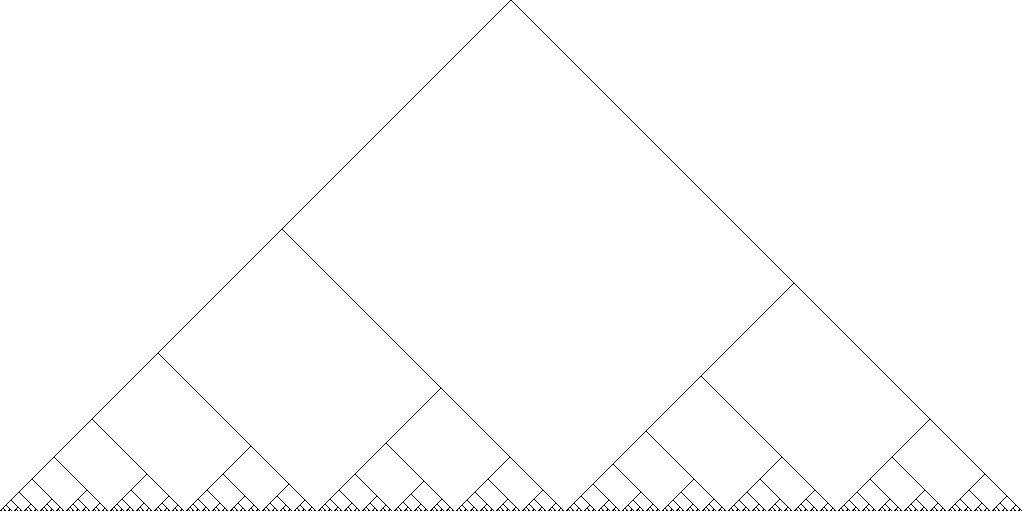
\includegraphics[width=0.8\textwidth]{sidh/optimal.png}
  \caption{Optimal strategy for $n=512,p=4.6,q=2.8$.}
  \label{sidh:fig:optimal}
\end{figure}

However, it is also possible to mathematically characterize the
optimal strategies. Since the optimal strategies for~$(p,q)$ are
symmetrical to those for~$(q,p)$, we may assume that~$p < q$. For
simplicity, we will also assume that $p$ and $q$ are integers: the
generalization to the case of rational $p$ and $q$ is
straightforward.

Let~$(u_m)$ be the sequence defined by~$u_{p+1} =
\dots = u_{p+q} = 1$ and~$u_m = u_{m-p} + u_{m-q}$, and~$f(n)$ be the
function defined by~$f(1) = 0$, $f(n) = f(u_{m}) + m(n - u_m)$
for all~$n \in [u_{m}, u_{m+1}]$. We check that $f$~satisfies the
recurrence relation
\begin{equation}\label{sidh:eq:recurrence-f}
f(u_m) = f(u_{m-p}) + f(u_{m-q}) + p u_{m-p} + q u_{m-q}.
\end{equation}

\begin{proposition}\label{sidh:prop:optimal-strategy}
A full strategy~$S$ is optimal if, and only if, it is canonical, both its left
and right branches~$S'$ and~$S''$ are optimal, and
\[ u_{m-q} \leq \abs{S'} \leq u_{m-q+1}, \quad
  u_{m-p} \leq \abs{S''} \leq u_{m-p+1}, \]
where $m$~is such that~$u_{m} \leq \abs{S} < u_{m+1}$. In this case, the
weight of~$S$ is~$f(\abs{S})$.
\end{proposition}

For example, in the case where~$p = 1$ and~$q = 2$, the sequence~$(u_m)$
is the sequence of Fibonacci numbers, starting at~$u_2 = 1$, $u_3 = 1$,
$u_4 = 2$..., and a strategy~$S$ with~$u_{m} \leq \abs{S} < u_{m+1}$ is
optimal if, and only if, the left and right branches~$S'$ and~$S''$
satisfy $u_{m-2} \leq \abs{S'} \leq u_{m-1}$ and~$u_{m-1} \leq \abs{S''} \leq
u_m$.

\begin{proof}
We prove this by induction on~$n = \abs{S}$. Let~$n = n' + n''$ with~$n',
n'' > 0$ and let~$S = S_{n',n''}$ be any canonical full strategy with optimal
left and right branches~$S'$, $S''$, such that~$\abs{S'} = n'$
and~$\abs{S''} = n''$. Then any optimal strategy is one of
the~$S_{n',n''}$. Therefore, we find them by looking at the sign
of~$\delta_n = (S_{n'+1,n''-1}) - (S_{n',n''})$.

Let~$m',m''$ be such that~$u_{m'} \leq n' < u_{m' + 1}$ and~$u_{m''} \leq
n'' < u_{m''+1}$. Using the induction hypothesis on~$S'$ and~$S''$, we
have $(S_{n',n''}) = f(n') + f(n'')  + n' q + n'' p$, and therefore
\begin{equation}
\delta_n \;=\; \begin{cases}
(m' + q) - (m'' + p),& \text{if $n'' \geq u_{m''} + 1$,}\\
(m' + q) - (m'' + p) + 1, &\text{if $n'' = u_{m''}$.}
\end{cases}
\end{equation}
We find that~$\delta_n \leq 0$ exactly when~$n' < u_{m-q+1}$ and~$n'' >
u_{m-p}$, and $\delta_n \geq 0$ exactly when~$n' \geq u_{m-q}$ and~$n''
\leq u_{m-p+1}$. The optimality condition follows from this.
It remains only to check that~$(S) = f(\abs{S})$: this results from
relation~(\ref{sidh:eq:recurrence-f}).
\end{proof}

In particular, there are in general several optimal strategies of a given
size. Moreover, with~$z$ being the (unique) root in~$[0,1]$ of the
equation~$z^p + z^q - 1 = 0$, this gives the asymptotic equivalents
\begin{eqnarray}
\abs{S'} &\sim& z^q \abs{S},\\
C_{p,q}(n) = (S) &\sim& -\frac{1}{\log z}\, n \log n.
\end{eqnarray}
The relative cost of an optimal strategy is therefore
asymptotically~$-\frac{2 \log 2}{\log (z^{p+q})}$ times the cost of
the balanced strategy. In the case where~$(p, q) = (4.6, 2.8)$, as in
Table~\ref{sidh:tab:counts} with~$\ell = 2$, this gives an improvement
of~2.1\% over the balanced strategy.

\subsection{Choice of the models}\label{sidh:subsec:montgomery}

At each phase of the key generation it is important to use models for
elliptic curves that offer the fastest formulas for doubling,
addition, isogeny computation and evaluation, etc.

To measure efficiency, we count the number of elementary operations in
$\FF_{p^2}$: we write $I,M,S$ for the costs of one inversion,
multiplication and squaring respectively, and we make the assumption
$S\le M\le I$. We neglect additions, subtractions and comparisons. We
refer to the Explicit Formulas Database (EFD)~\cite{efd} for operation
counts of elliptic point addition, doubling, etc. in various models
and coordinate systems. Contrary to the convention taken in the EFD,
we count multiplications by constants (other than small integers) as
ordinary multiplications.

Any curve used in our cryptosystem has group structure
$\left(\ZZ/(p\mp 1)\ZZ\right)^2$. Hence either the curve or its twist
has a point of order~$4$. Consequently, it is isomorphic to a twisted
Edwards curve and to a Montgomery curve~\cite{twisted-edwards}.

Twisted Edwards curves~\cite{twisted-edwards} have equation
\begin{equation}
  \label{sidh:eq:twisted-ed}
  E_{a,d}\;:\;ax^2+y^2=1+dx^2y^2.
\end{equation}
They have many interesting properties, but what interests us most is
their very efficient addition and doubling formulas.  Using projective
coordinates, one point addition costs $12M+1S$ and one point doubling
costs $4M+4S$. When one of the points is scaled to have $Z$-coordinate
equal to $1$, these costs drop to $11M+1S$ and $3M+4S$ respectively.

Montgomery curves~\cite{montgomery} have equation
\begin{equation}
  \label{sidh:eq:montgomery}
  M_{B,A}\;:\;By^2 = x^3 + Ax^2 + x.
\end{equation}
They have very efficient arithmetic on their Kummer line, i.e., by
representing points by the coordinates $(X:Z)$ where $x=X/Z$.  Using
this representation, a point can be doubled using $3M+2S$, or $2M+2S$
when it is scaled to have $Z$-coordinate equal to $1$.

The Kummer line identifies $P$ with $-P$; thus it is not possible to
add two distinct points. However it is still possible to perform what
is called \emph{differential addition}, i.e., adding points $P$ and
$Q$ for which the difference $P-Q$ is known. One differential addition
can be computed using $4M+2S$, or $3M+2S$ when the difference $P-Q$ is
scaled to have $Z$-coordinate equal to $1$.

By using doublings and differential additions, it is possible to
compute any scalar multiple of a point using a Montgomery
ladder~\cite{montgomery}. Also observe that since $P$ and $-P$
generate the same subgroup, isogenies can be defined and evaluated
correctly on the Kummer line. We shall give formulas for this
operation later.

It is shown in~\cite{twisted-edwards} that the twisted Edwards curve
$E_{a,d}$ is birationally equivalent to the Montgomery curve $M_{A,B}$
where
\begin{equation}
  A = \frac{2(a+d)}{a-d}, \qquad B = \frac{4}{a-d},
\end{equation}
and where the transformation is given by the following maps (in
affine coordinates)
\begin{equation}
  \label{sidh:eq:birational}
  \begin{aligned}
    \psi\;:\;E_{a,d}&\to M_{A,B},\\
    (x,y) &\mapsto \left(\frac{1+y}{1-y}, \frac{1+y}{(1-y)x}\right),
  \end{aligned}
  \qquad
  \begin{aligned}
    \psi^{-1}\;:\;M_{A,B}&\to E_{a,d},\\
    (x,y) &\mapsto \left(\frac{x}{y}, \frac{x-1}{x+1}\right).
  \end{aligned}
\end{equation}
Hence, after the models $E_{a,d}$ and $M_{A,B}$ are computed, points
in projective coordinates can be moved from one model to the other at
a cost of a few multiplications (and no inversions).

Now we detail the cost of each step of the key generation algorithm.

\subsubsection{Computing $\cyc{[m]P+[n]Q}$}\label{sidh:sssec:montgomery-ladder}

We have already mentioned two algorithms to compute the value of
$P+[m^{-1}n]Q$. One solution is to express the points $P$ and $Q$ in
projective Edwards coordinates and perform a double and add followed
by an addition. If we scale $Q$ to have $Z$-coordinate equal to $1$,
computing $[m^{-1}n]Q$ costs $9.5M+4.5S$ per bit on average.

Because addition by $P$ is performed last, this approach cannot
be used with points on the Montgomery curve in Kummer coordinates, but
we can use the ladder given in Algorithm~\ref{sidh:fig:ladder} instead. We
first compute $P-Q$ using point addition in full projective
coordinates (either by using the standard chord-and-tangent law, or by
using the equivalence with twisted Edwards curves). Then we scale $P$,
$Q$ and $P-Q$ to have $Z$-coordinate equal to $1$. We can now discard
the $Y$ coordinate and work on the Kummer line. At each iteration we
perform one doubling and two differential additions (with one of the
scaled points $P$, $Q$ and $P-Q$). The total cost of one iteration is
thus $9M+6S$.

In general the cost of one squaring is close to the cost of one
multiplication. Thus the ladder algorithm is slightly slower than
double-and-add. However the advantages of the ladder are SPA
resistance and an implementation simplified by not using Edwards
coordinates at all for key generation.

\subsubsection{Isogenies of Montgomery curves}\label{sidh:sssec:montgomery-isogeny}

The literature on efficient formulas for evaluating small degree
isogenies is much less extensive than for point multiplication. We now
give explicit formulas for isogenies of Montgomery curves, and
optimize the degree $2$ and $3$ cases. Our goal is to obtain the most
efficient formulas for isogeny evaluation, and thus we seek to avoid
inversions and square root computations as much as possible.

Let $E$ be the Montgomery curve defined by Eq.~\eqref{sidh:eq:montgomery}.
It has a point of order two $P_2=(0,0)$, and a point of order four
$P_4=(1,\sqrt{(A+2)/B})$---sometimes defined over a quadratic
extension---such that $[2]P_4=P_2$. Montgomery curves have twists of
the form $\tilde{y}=\sqrt{c}y$; these are isomorphisms when $c$ is a
square. The change of coordinates $\tilde{x}=x/B, \tilde{y}=y/B$
brings the curve $E$ to the Weierstrass form
\begin{equation}
  \label{sidh:eq:twisted}
  \tilde{y}^2 = \tilde{x}^3 + \frac{A}{B}\tilde{x}^2 + \frac{1}{B^2}\tilde{x},
\end{equation}
and the point $P_4$ to $P_4'=(1/B,\ldots)$. Conversely, given a
Weierstrass curve with equation
$\tilde{y}^2=\tilde{x}^3+a\tilde{x}^2+b\tilde{x}$, together with a
point $P_4=(1/\beta,\ldots)$---with its ordinate possibly lying in a
quadratic extension---such that $[2]P_4=(0,0)$, the change of
variables $\tilde{x}=x/\beta, \tilde{y}=y/\beta$ brings the curve to
the Montgomery form $\beta y^2=x^3+a\beta x^2 + x$.

Given a point $P\ne\pm P_4$ of order $4$, we will need to compute the
isomorphism of Montgomery curves that brings $[2]P$ in $(0,0)$ and $P$
in $(1,\ldots)$. Let $X$ be the abscissa of $P$ and $X_0$ the abscissa
of $[2]P$; by a straightforward calculation, we find that this
isomorphism is given by the map
\begin{equation}
  \label{sidh:eq:isomorphism}
  \begin{aligned}
    \iota : E &\to E',\\
    (x,y) &\mapsto \left(\frac{x-X_0}{X-X_0}, \frac{y}{X-X_0}\right),
  \end{aligned}
\end{equation}
and the new curve has equation
\begin{equation*}
  E' \;:\; \frac{B}{X-X_0}y^2 = x^3 + \frac{3X_0 + A}{X-X_0} x^2 + x.
\end{equation*}

By precomputing $1/(X-X_0)$, and sharing common subexpressions, the
above map can be evaluated on a point in full projective
coordinates using $3M$ operations, or $2M$ using Kummer
coordinates.

Let $G$ be a subgroup of the Montgomery curve $E$ of odd cardinality
$\ell$ and let $h$ be the degree $(\ell-1)/2$ polynomial vanishing on
the abscissas of $G$. With a twist $y=\tilde{y}/\sqrt{B}$, we can put
$E$ in the form
\begin{equation*}
  E \;:\; \tilde{y}^2 = \tilde{x}^3 + A\tilde{x}^2 +\tilde{x},
\end{equation*}
and this does not change the abscissas of $G$ nor the polynomial
$h$. Now, composing the twist with V\'elu's formulas gives an isogeny
\begin{equation*}
  \begin{aligned}
    \phi : E &\to E/G,\\
    (x,y) &\mapsto \left(\frac{g(x)}{h(x)^2}, y\sqrt{B}\left(\frac{g(x)}{h(x)^2}\right)'\right).
  \end{aligned}
\end{equation*}

We now need to express $E/G$ in Montgomery form. Because $\ell$ is
odd, the point $(0,0)$ of $E$ is sent to a point of order two in
$E/G$, and the change of variables
$\tilde{x}=x-g(0)/h(0)^2$ brings this point to $(0,0)$.

Now, $\phi(P_4)$ is a point of order four lying above $(0,0)$ (possibly
in a quadratic extension). Its abscissa is rational and is given by
\begin{equation}
  \frac{1}{\beta} = \frac{g(1)}{h(1)^2} - \frac{g(0)}{h(0)^2},  
\end{equation}
so we further apply the change of variables
$\tilde{x}=\bar{x}/\beta,\tilde{y}=\bar{x}/\beta$ to obtain a
Montgomery curve. Finally, we have to twist back the model in order to
obtain a curve isogenous over the base field: the twist $\bar{y} =
y\sqrt{B}$ cancels with the first one and leaves us with
square-root-free formulas.

Given $h$ as input, the cost of evaluating the whole path is $O(\ell)$
operations in the base field, using the formula in
\cite[Proposition~4.1]{bostan+morain+salvy+schost08} to evaluate $g/h$.

Let now $P$ be a $3$-torsion point, let $G=\{0,P,-P\}$ and let $X$ be
the abscissa of $P$ (and $-P$). If we specialize the formula to the
case $\ell=3$, we have $h = x - X$ and
\begin{equation}
  \label{sidh:eq:3-isogeny}
  \begin{aligned}
    \phi : E &\to E/G,\\
    (x,y) &\mapsto \textstyle{\left(
      \frac{x\left(x - \frac{1}{X}\right)^2}{(x-X)^2}X^2,\;
      y\frac{\left(x-\frac{1}{X}\right)\left(\left(x-\frac{1}{X}\right)(x-X)+2x\left(\frac{1}{X}-X\right)\right)}{(x-X)^3}X^2
    \right),}
  \end{aligned}
\end{equation}
and the curve $E/G$ has equation
\begin{equation*}
  E/G \;:\; BX^2y^2 = x^3 + \left(A+\frac{6}{X}-6X\right)X^2x^2 + x.
\end{equation*}

By precomputing $X$ and $X^2$, and sharing common subexpressions, the
above isogeny can be evaluated on a point in full projective
coordinates using $11M+2S$ operations, or $4M + 2S$ using Kummer
coordinates.

When $\ell$ is even, things get more complicated. Recall that
$P_2=(0,0)$ and $P_4=(1,\sqrt{(A+2)/B})$. The isogeny of degree $2$
vanishing on $P_2$ and mapping $P_4$ to $(0,0)$ is readily seen as
being
\begin{align}
  \label{sidh:eq:isogeny-2}
  &F \;:\;  By^2 = x^3 + (A+6)x^2 + 4(2+A)x,\\
  &\begin{aligned}
    \phi : E &\to F,\\
    (x,y) &\mapsto \left(\frac{(x-1)^2}{x}, y\left(1 - \frac{1}{x^2}\right)\right).
  \end{aligned}
\end{align}
It is not immediately evident how to put $F$ in Montgomery form
without computing square roots. Let $P_8$ be a point satisfying
$[2]P_8=P_4$. Then we have $\phi(P_8)=(2\sqrt{2+A},\ldots)$, and $F$ can be
put in the form
\[\frac{B}{2\sqrt{2+A}}y^2 = x^3 + \frac{A+6}{2\sqrt{2+A}}x^2 + x,\]
with the point $(1,\ldots)$ being the image of $P_8$.  Any other
isogeny of degree $2$ can be treated by applying
Eq.~\eqref{sidh:eq:isomorphism} to move the generator of the kernel in
$(0,0)$.

By precomputing $1/\phi(P_8)$, and sharing common subexpressions, the
above isogeny can be evaluated on a point in full projective
coordinates using $5M+3S$ operations, or $2M+S$ using Kummer
coordinates. Unfortunately, this formula takes no square roots only if
an $8$-torsion point above $P_2$ is known.


Alternatively, $\phi$ and $F$ being as before, we consider the isogeny
$\psi:F\to F/\cyc{(0,0)}$ given by
\begin{align}
  \label{sidh:eq:isogeny-4}
  &G \;:\;  \frac{B}{2-A}y^2 = x^3 - 2\frac{A+6}{2-A}x^2 + x,\\
  &\begin{aligned}
    \psi : F &\to G,\\
    (x,y) &\mapsto \left(\frac{1}{2-A}\frac{(x+4)(x+(A+2))}{x}, \frac{y}{2-A}\left(1 - \frac{4(2+A)}{x^2}\right)\right).
  \end{aligned}
\end{align}
Then $\phi_4 = \psi\circ\phi$ is an isogeny of degree four
$\phi_4\colon E\to
E/\cyc{P_4}$, and the point $\left(1,\sqrt{-4(A+2)/B}\right)$ of $G$
generates the kernel of the dual isogeny $\hat{\phi}_4$. Any other
isogeny of degree $4$ can be treated by applying
Eq.~\eqref{sidh:eq:isomorphism} to move the kernel point to $(1,\ldots)$.

By precomputing $1/(2-A)$, and sharing common subexpressions, the
isogeny $\phi_4$ can be evaluated on a point in full projective
coordinates using $10M+4S$ operations, or $4M+S$ using Kummer
coordinates.

Unfortunately, this formula cannot be applied twice to obtain a degree
$16$ cyclic isogeny: indeed, a double application yields the
multiplication-by-$4$ isogeny. If a chain of degree $4$ isogenies is
wanted, as for the algorithm in Subsection~\ref{sidh:sssec:isogeny}, this
formula must be combined with the isomorphism in
Eq.~\eqref{sidh:eq:isomorphism}.

Isogenies of composite smooth degree are computed by composing small
degree isogenies as discussed in Subsection~\ref{sidh:sssec:isogeny}. We
focus on the fine tuning of this algorithm when the small isogenies
have degrees $2,3$ and $4$.

It is important to remark that, after a generator $R$ of the kernel of
the isogeny has been computed, the algorithm does not use its ordinate
at all: indeed, all the previous formulas for small degree isogenies
only use the abscissas of the kernel points. Hence, we can throw away
the ordinate of $R$ altogether and only use scalar multiplication and
isogeny evaluation formulas for points in Kummer
coordinates.

As usual, some more care must be taken when computing cyclic isogenies
of degree $2^e$. In principle, one could compose either degree $2$
(Eq.~\ref{sidh:eq:isogeny-2}) or degree $4$ (Eq.~\ref{sidh:eq:isogeny-4})
isogenies; however we have already pointed out some caveats:

\begin{itemize}
\item Both equations require the kernel point to be moved to some
  specific coordinates. This can be achieved using the isomorphism in
  Eq.~\eqref{sidh:eq:isomorphism}.
\item After the first change of variables, Eq.~\eqref{sidh:eq:isogeny-2}
  can be repeatedly chained with itself; however, from a point of
  order $2^e$ only $e-2$ degree $2$ isogenies can be computed this
  way, because the formula requires the knowledge of a point of order $8$.
\item Eq.~\eqref{sidh:eq:isogeny-4} cannot be directly chained with itself
  to compute a cyclic isogeny of degree $4^e$. It must be composed,
  instead, with Eq.~\eqref{sidh:eq:isomorphism} at each step.
\end{itemize}

Having this in mind, two obvious strategies to compute degree $2^e$
isogenies are:

\begin{enumerate}
\item Use degree $2$ isogenies as much as possible; use one degree $4$
  isogenies for the last two steps.
\item Use one degree $2$ isogeny if $e$ is odd, then use only degree
  $4$ isogenies composed with isomorphisms.
\end{enumerate}

Table~\ref{sidh:tab:strategies} below suggests that the second strategy
yields a very small improvement over the first. The experiments of
Section~\ref{sidh:sec:imp} show that operations not accounted for in this
analysis might give a greater advantage to the second
strategy. However, for lack of time, we only implemented the first
one.

Finally, it should be noted that both approaches, if implemented as
described above, leak two bits of security. Indeed, the point
$(1,\ldots)$ of the image curve is a point of order $4$ in the kernel
of the dual of the computed isogeny (the secret). It is easy to mask
this leakage by taking a random change of coordinates. However, for
practical purposes, we found this masking more costly than simply adding
two bits of security and letting the information leak, although
technically the
leaked information alters the complexity assumptions needed for the
security proofs. For ease of analysis, we assume in
Section~\ref{sidh:sec:security} that coordinate masking has been applied.

Table~\ref{sidh:tab:counts} summarizes the costs of the isogeny evaluation
and scalar multiplication formulas in light of these remarks. Because
squaring in $\FF_{p^2}$ is faster than multiplication, we also report
the cost obtained by taking $S=0.8M$ (a factor that roughly
approximates the fact that squaring requires $2$ multiplications in
$\FF_p$ instead of $3$).

Table~\ref{sidh:tab:strategies} compares the total cost of isogeny
evaluations and scalar multiplications in a balanced and an optimal
strategy for $\ell=2,3,4$, based on the costs given in
Table~\ref{sidh:tab:counts}, at the classical 256-bit security level (see
Section~\ref{sidh:sec:security} for our complexity assumptions). We make the following observations, backed up by the benchmarks in Section~\ref{sidh:sec:imp}:
\begin{itemize}
\item There may be a small advantage (less than $2\%$) in using
  isogenies of degree $4$ instead of $2$;
\item The gain in using an optimal strategy instead of a balanced one
  is consistent with the predictions of
  Subsection~\ref{sidh:sssec:isogeny};
\item The difference between $2^e$ and $3^e$ isogenies is more
  significant (about $20\%$), suggesting that degree $2^e$ isogenies
  may be preferable for constrained devices.
\end{itemize}

\begin{table}[t]
  \centering
  \caption{Comparative costs for multiplication and isogeny evaluation in projective Kummer coordinates, in number of multiplications and squarings, and assuming $S=0.8M$.}
  \label{sidh:tab:counts}
  \begin{tabular}{ l @{\hspace{1ex}} | *{3}{@{\hspace{1em}} r} }
    $\ell$ & $2$ & $3$ & $4$ \\
    \hline
    Isogeny & $2M+S$ & $4M+2S$ & $6M+S$\\
            &  $2.8$ &   $5.6$ &  $6.8$\\
    \hline
    Multiplication & $3M+2S$ & $7M+4S$ & $6M+4S$\\
                   &   $4.6$ &  $10.2$ &   $9.2$
  \end{tabular}
\end{table}


\begin{table}[t]
  \centering
  \caption{Comparative costs of the balanced and the optimal strategies for computing a degree $2^{514}$ ($\ell=2,4$) or $3^{323}$ ($\ell=3$) isogeny, assuming $S=0.8M$.}
  \label{sidh:tab:strategies}
  \begin{tabular}{ l | *{3}{r} | *{3}{r} }
    & \multicolumn{3}{c|}{optimal strategy} & \multicolumn{3}{c}{balanced strategy}\\
    $\ell$ & $2$ & $3$ & $4$ & $2$ & $3$ & $4$\\
    \hline
    Isogenies       & $2741$    & $1610$    & $1166$    & $2323$    & $1430$    & $1033$ \\
    Multiplications & $1995$    & $1151$    & $921$     & $2307$    & $1288$    & $1025$ \\
    Total cost      & $16852$ & $20756$ & $16402$ & $17117$ & $21146$ & $16454$
  \end{tabular}
\end{table}


\section{Complexity assumptions}\label{sidh:sec:security}

As before, let $p$ be a prime of the form $\ell_A^{e_A}
\ell_B^{e_B}\cdot f \pm 1$, and fix a supersingular curve $E_0$ over
$\FF_{p^2}$ together with bases $\{P_{A},Q_{A}\}$ and
$\{P_{B},Q_{B}\}$ of $E_0[\ell_A^{e_A}]$ and $E_0[\ell_B^{e_B}]$
respectively. In analogy with the case of isogenies over ordinary
elliptic curves, we define the following computational problems,
adapted for the supersingular case:

\begin{problem}[Decisional Supersingular Isogeny (DSSI) problem] Let
  $E_A$ be another supersingular curve defined over
  $\FF_{p^2}$. Decide whether $E_A$ is $\ell_A^{e_A}$-isogenous to
  $E_0$.
\end{problem}

\begin{problem}[Computational Supersingular Isogeny (CSSI) problem]
Let the map $\phi_A \colon E_0 \to E_A$ be an isogeny whose kernel is
$\cyc{[m_A]P_A+[n_A]Q_A}$, where $m_A$ and $n_A$ are chosen at random
from $\ZZ/\ell_A^{e_A}\ZZ$ and not both divisible by $\ell_A$.  Given
$E_A$ and the values $\phi_A(P_B)$, $\phi_A(Q_B)$, find a generator
$R_A$ of $\cyc{[m_A]P_A+[n_A]Q_A}$.
\end{problem}

We remark that given a generator $R_A = [m_A]P_A+[n_A]Q_A$, it is easy
to solve for $(m_A,n_A)$, since $E_0$ has smooth order and thus
extended discrete logarithms are easy in $E_0$~\cite{teske-ph}.

\begin{problem}[Supersingular Computational Diffie-Hellman
    (SSCDH) problem] Let $\phi_A \colon E_0 \to E_A$ be an isogeny
  whose kernel is equal to $\cyc{[m_A]P_A+[n_A]Q_A}$, and let $\phi_B \colon
  E_0 \to E_B$ be an isogeny whose kernel is
  $\cyc{[m_B]P_B+[n_B]Q_B}$, where $m_A,n_A$ (respectively $m_B,n_B$)
  are chosen at random from $\ZZ/\ell_A^{e_A}\ZZ$ (respectively
  $\ZZ/\ell_B^{e_B}\ZZ$) and not both divisible by $\ell_A$ (respectively
  $\ell_B$). Given the curves $E_A,$ $E_B$ and the points
  $\phi_A(P_B),$ $\phi_A(Q_B),$ $\phi_B(P_A),$ $\phi_B(Q_A)$, find the
  $j$-invariant of $E_0/\cyc{[m_A]P_A+[n_A]Q_A ,[m_B]P_B+[n_B]Q_B}$.
\end{problem}

\begin{problem}[Supersingular Decision Diffie-Hellman (SSDDH)
    problem] Given a tuple sampled with probability $1/2$ from one of
  the following two distributions:
\begin{itemize} 
\item $(E_A, \phi_A(P_B), \phi_A(Q_B), E_B, \phi_B(P_A), \phi_B(Q_A),
  E_{AB})$, wherein the quantities $E_A,$ $\phi_A(P_B),$ $\phi_A(Q_B),$ $E_B,$
  $\phi_B(P_A),$ and $\phi_B(Q_A)$ are as in the SSCDH problem and \[E_{AB} \iso
  E_0/\cyc{[m_A]P_A+[n_A]Q_A ,[m_B]P_B+[n_B]Q_B},\]
\item $(E_A, \phi_A(P_B), \phi_A(Q_B), E_B, \phi_B(P_A), \phi_B(Q_A),
  E_C)$, wherein the quantities $E_A,$ $\phi_A(P_B),$ $\phi_A(Q_B),$ $E_B,$
  $\phi_B(P_A),$ and $\phi_B(Q_A)$ are as in the SSCDH problem and \[E_{C} \iso
  E_0/\cyc{[m_A']P_A+[n_A']Q_A ,[m_B']P_B+[n_B']Q_B},\] where
  $m_A',n_A'$ (respectively $m_B',n_B'$) are chosen at random from
  $\ZZ/\ell_A^{e_A}\ZZ$ (respectively $\ZZ/\ell_B^{e_B}\ZZ$) and not both
  divisible by $\ell_A$ (respectively $\ell_B$),
\end{itemize}
determine from which distribution the tuple is sampled.
\end{problem}

The ordinary case analogue of the following problem is trivially
solvable in polynomial time. Its supposed difficulty in the
supersingular case is at the heart of the security of our
identification scheme.

\begin{problem}[Decisional Supersingular Product (DSSP) problem]
  Given a degree $\ell_A^{e_A}$ isogeny $\phi:E_0\to E_3$ and a
  tuple sampled with probability $1/2$ from one of the following two
  distributions:
  \begin{itemize} 
  \item $(E_1,E_2,\phi')$, where the product $E_1\times E_2$ is chosen
    at random among those $\ell_B^{e_B}$-isogenous to $E_0\times E_3$,
    and where $\phi':E_1\to E_2$ is an isogeny of degree
    $\ell_A^{e_A}$, and
  \item $(E_1,E_2,\phi')$, where $E_1$ is chosen at random among the
    curves having the same cardinality as $E_0$, and $\phi':E_1\to
    E_2$ is a random isogeny of degree $\ell_A^{e_A}$,
  \end{itemize}
  determine from which distribution the tuple is sampled.
\end{problem}

We conjecture that these problems are computationally infeasible, in
the sense that for any polynomial-time solver algorithm, the advantage
of the algorithm is a negligible function of the security parameter
$\log p$. The resulting security assumptions are referred to as the
DSSI assumption, CSSI assumption, etc.


\subsection{Hardness of the underlying
  assumptions}\label{sidh:subsec:hardness}

Given a CSSI (respectively, SSCDH) solver, it is trivial to solve
SSCDH (respectively, SSDDH). It is also trivial to solve SSDDH given a
DSSI solver. There are no known reductions in the other direction, and
given that the corresponding question of equivalence for discrete
logarithms and Diffie-Hellman has not yet been completely resolved in
all cases, it is reasonable to assume that the question of equivalence
of CSSI, SSCDH, and SSDDH is at least hard to resolve. For the
purposes of this discussion, we will presume that DSSI and CSSI are
equivalent to SSDDH. Concerning DSSP, there is an evident reduction to
DSSI. However, it seems reasonable to assume that DSSP is easier than the
latter.

In the context of cryptography, the problem of computing an isogeny
between isogenous supersingular curves was first considered by
Galbraith~\cite{Gal} in 1999. The first published cryptographic
primitive based on supersingular isogeny graphs is the hash function
proposal of Charles et al.~\cite{charles+lauter+goren09}, which remains unbroken to date
(the cryptanalysis of~\cite{quis} applies only to the LPS graph-based
hash function from~\cite{charles+lauter+goren09}, and not to the supersingular isogeny
graph-based hash functions). The fastest known algorithm for finding
isogenies between supersingular curves in general takes $O(\sqrt{p}
\log^2 p)$ time~\cite[\S 5.3.1]{charles+lauter+goren09}; however our problem is less
general because the degree of the isogeny is known in advance and is
smooth. In addition, the distribution of isogenous
  curves obtained
from taking kernels of the form $\cyc{[m_A]P_A+[n_A]Q_A}$ is not quite
uniform: a simple calculation against Proposition~\ref{sidh:prop:mixing}
indicates that a sequence of $e_A$ isogenies of degree $\ell_A$ falls
short of the length needed to ensure uniform mixing, regardless of the
value of $p$. Since we are the first to propose using isogenies of
this type, there is no existing literature addressing the security
of the isogenies of the special form that we propose.

There are easy exponential attacks against DSSI and CSSI that improve
upon exhaustive search. To find an isogeny of degree $\ell_A^{e_A}$
between $E$ and $E_A$, an attacker builds two trees of all curves
isogenous to $E$ (respectively, $E_A$) via isogenies of degree
$\ell_A^{e_A/2}$. Once the trees are built, the attacker tries to find
a curve lying in both trees. Since the degree of the isogeny $\phi_A$
is $\sim\sqrt{p}$ (much shorter than the size of the isogeny graph),
it is unlikely that there will be more than one isogeny path---and
thus more than one match---from $E$ to $E_A$. Given two functions
$f:A\to C$ and $g:B\to C$ with domain of equal size, finding a pair
$(a,b)$ such that $f(a)=g(b)$ is known as the \emph{claw problem} in
complexity theory. The claw problem can obviously be solved in $O(|A|
+ |B|)$ time and $O(|A|)$ space on a classical computer by building a
hash table holding $f(a)$ for any $a\in A$ and looking for hits for
$g(b)$ where $b\in B$. This gives a $O(\ell_A^{e_A/2})=O(\sqrt[4]{p})$
classical attack against our cryptosystems. With a quantum computer,
one can do better using the algorithm in~\cite{tani2009claw}, which has
complexity $O(\sqrt[3]{|A||B|})$, thus giving an
$O(\ell_A^{e_A/3})=O(\sqrt[6]{p})$ quantum attack against our
cryptosystems. These complexities are optimal for a black-box claw
attack~\cite{zhang}.

We consider the question of whether the auxiliary data points
$\phi_A(P_B)$ and $\phi_A(Q_B)$ might assist an adversary in
determining $\phi_A$. Since $(P_B,Q_B)$ forms a basis for
$E_0[\ell_B^{e_B}]$, the values $\phi_A(P_B)$ and $\phi_A(Q_B)$ allow
the adversary to compute $\phi_A$ on all of $E_0[\ell_B^{e_B}]$. This
is because any element of $E_0[\ell_B^{e_B}]$ is a (known) linear
combination of $P_B$ and $Q_B$ (known since extended discrete
logarithms are easy~\cite{teske-ph}). However, there does not appear
to be any way to use this capability to determine $\phi_A$. Even on a
quantum computer, where finding abelian hidden subgroups is easy,
there is no hidden subgroup to find, since $\phi_A$ has degree
$\ell_A^{e_A}$, and thus does not annihilate any point in
$E_0[\ell_B^{e_B}]$ other than the identity. Of course, if one could
evaluate $\phi_A$ on arbitrary points of $E_0[\ell_A^{e_A}]$, then a
quantum computer could easily break the scheme, and indeed in this case the
scheme is also easily broken classically by using a few calls to the
oracle to compute a generator of the kernel of the dual isogeny 
$\hat{\phi}_A$. However, it does not seem possible to translate the values of
$\phi_A$ on $E_0[\ell_B^{e_B}]$ into values on $E_0[\ell_A^{e_A}]$.

For both ordinary and supersingular curves, there is a natural
bijection between isogenies (up to isomorphism) and (left) ideals in
the endomorphism ring. In the ordinary case the endomorphism ring is
commutative, and ideal classes form a finite abelian group. This
property has been used by Childs et al.~\cite{childs2014constructing} to solve the
ordinary analogue of CSSI in quantum subexponential time. It is
natural to ask whether their algorithm can be adapted to the
supersingular setting. Here the
endomorphism ring is a maximal order in a noncommutative quaternion
algebra, and the left ideal classes do not form a group at all (though
they do
form a groupoid). Since the algorithm of Childs et al. depends
crucially on the properties of abelian groups, we believe that no
reasonable variant of this strategy would apply.

The same correspondence between isogenies and ideals can be applied to
DSSP. Indeed, deciding DSSP amounts to deciding whether the ideals
$S,S'$ associated to $\phi,\phi'$ are conjugated, i.e., whether there
exists a left ideal $R\in\End(E_0)$ such that $S=RS'R^{-1}$. Although
it can be hoped that deciding conjugacy of ideal classes in the
quaternion algebra $\QQ_{p,\infty}$ is feasible, we are still faced
with the problem that the best known algorithms to compute the
endomorphism rings of supersingular curves are exponential in $\log
p$~\cite{kohel,cervino04,belding08-thesis}. Hence, we deem DSSP secure
given the current knowledge.

The fact that it is possible to obtain a zero-knowledge identification
scheme from CSSI comes as no surprise, since it is well known that a
zero-knowledge protocol can be obtained from any problem in
NP~\cite{goldreich+micali+widgerson91}. Nevertheless, the generic
construction is not very efficient, and many efforts have been made to
obtain efficient \emph{ad-hoc} schemes from NP-complete
problems~\cite{shamir89-pkp,stern94-CLE,stern94-SD,pointcheval95-pp}. While
the security of most of these schemes is based on two solid
assumptions, namely that P $\ne$ NP and that \emph{secure commitment
  schemes} exist, our identification scheme stands on a much
weaker ground: the CSSI and DSSP problems. As performances go, it is
reasonable to assume that our scheme will be some orders of magnitude
slower than the best zero-knowledge protocols. We can thus conclude
that our scheme is of a purely theoretical and pedagogical interest.
Yet it is remarkable that an efficient identification scheme based on
graphs of supersingular isogenies simply exists, while the analogous
construction for ordinary curves is trivially broken and no other
identification scheme is currently known to work in that
case~\cite{Stol}.

\section{Security proofs}\label{sidh:sec:proof}



In this section we state formal security reductions relating the
security of our protocols to the hardness of the appropriate
underlying isogeny computation problem. The security proofs are
routine, but tedious, and contain little original contribution on
our part. For this reason, we only prove a representative selection
of our theorems.

The statements of the theorems are as follows:

\begin{theorem}\label{sidh:thm:kep-proof}
If the SSDDH assumption holds, then the key-agreement protocol of
Section~\ref{sidh:subsec:kep} is session-key secure in the
authenticated-links adversarial model of Canetti and
Krawczyk~\cite{canetti}.
\end{theorem}
\begin{theorem}\label{sidh:thm:pk-proof}
If the SSDDH assumption holds, and the hash function family
$\mathcal{H}$ is entropy-smoothing, then the public-key cryptosystem
of Section~\ref{sidh:subsec:pk} is IND-CPA.
\end{theorem}
\begin{theorem}\label{sidh:thm:zk-proof}
  Under the CSSI and DSSP assumptions, the identification scheme of
  Section~\ref{sidh:subsec:zk} is zero-knowledge.
\end{theorem}

\subsection{Proof of Theorem~\ref{sidh:thm:kep-proof}}\label{sidh:subsec:zkp-proof}

The proofs of Theorems~\ref{sidh:thm:kep-proof} and~\ref{sidh:thm:pk-proof} are
easily adapted from the corresponding proofs given by
Stolbunov~\cite{stolbunov-red}. As an illustration of the proof
techniques, we provide a proof of Theorem~\ref{sidh:thm:kep-proof}.

We recall the definition of session-key security in the
authenticated-links adversarial model of Canetti and
Krawczyk~\cite{canetti}. We consider a finite set of \emph{parties}
$P_1, P_2, \ldots, P_n$ modeled by probabilistic Turing machines.  The
adversary $\mathcal{I}$, also modeled by a probabilistic Turing
machine, controls all communication, with the exception that the
adversary cannot inject or modify messages (except for messages from
corrupted parties or sessions), and any message may be delivered at
most once. Parties give outgoing messages to the adversary, who has
control over their delivery via the \textsf{Send} query. Parties are
activated by \textsf{Send} queries, so the adversary has control over
the creation of protocol sessions, which take place within each party.
Two sessions $s$ and $s'$ are \emph{matching} if the outgoing messages
of one are the incoming messages of the other, and vice versa.

We allow the adversary black-box access to the queries
$\mathsf{SessionStateReveal}$, $\mathsf{SessionKeyReveal}$, and
$\mathsf{Corrupt}$. The $\mathsf{SessionStateReveal}(\mathfrak{s})$
query allows the adversary to obtain the contents of the session
state, including any secret information. The query is noted and
$\mathfrak{s}$ produces no further output.  The
$\mathsf{SessionKeyReveal(\mathfrak{s})}$ query enables the adversary
to obtain the session key for the specified session $\mathfrak{s}$, so
long as $\mathfrak{s}$ holds a session key. The
$\mathsf{Corrupt(P_i)}$ query allows the adversary to take over the
party $P_i$, i.e.,\ the adversary has access to all information in
$P_i$'s memory, including long-lived keys and any session-specific
information still stored. A corrupted party produces no further
output. We say a session $\mathfrak{s}$ with owner $P_i$ is
\emph{locally exposed} if the adversary has issued
$\mathsf{SessionKeyReveal(\mathfrak{s})}$,
$\mathsf{SessionStateReveal(\mathfrak{s})}$, or
$\mathsf{Corrupt(P_i)}$ before $\mathfrak{s}$ is expired. We say
$\mathfrak{s}$ is \emph{exposed} if $\mathfrak{s}$ or its matching
session have been locally exposed, and otherwise we say $\mathfrak{s}$
is \emph{fresh}.

We allow the adversary $\mathcal{I}$ a single
$\mathsf{Test(\mathfrak{s})}$ query, which can be issued at any stage
to a completed, fresh, unexpired session $\mathfrak{s}$. A bit $b$ is
then picked at random. If $b=0$, the test oracle reveals the session
key, and if $b=1$, it generates a random value in the key
space. $\mathcal{I}$ can then continue to issue queries as desired,
with the exception that it cannot expose the test session. At any
point, the adversary can try to guess $b$. Let
$\operatorname{GoodGuess}^{\mathcal{I}}(k)$ be the event that
$\mathcal{I}$ correctly guesses $b$, and define \[
\operatorname{Advantage}^{\mathcal{I}}(k) = \max \left\{0, \left \vert
\operatorname{Pr}[\operatorname{GoodGuess}^{\mathcal{I}}(k)] - \frac 1
2 \right \vert \right\},\] where $k$ is a security parameter.

The definition of security is as follows:

\begin{definition}\label{sidh:def:kep}
A key exchange protocol $\Pi$ in security parameter $k$ is said to be
\emph{session-key secure} in the authenticated-links adversarial model
of Canetti and Krawczyk if for any polynomial-time adversary $\mathcal{I}$,
\begin{enumerate}
\item If two uncorrupted parties have completed matching sessions,
  these sessions produce the same key as output;
\item $\operatorname{Advantage}^{\mathcal{I}}(k)$ is negligible.
\end{enumerate}
\end{definition}

\begin{algorithm}[t]
\caption{SSDDH distinguisher}
\label{sidh:alg:distinguisher}
\begin{algorithmic}[1]
\REQUIRE $E_A, E_B, \phi_A(P_B), \phi_A(Q_B), \phi_B(P_A),
\phi_B(Q_A), E$
\STATE $r \stackrel{R}{\leftarrow} \{1,\ldots,k\}$, where $k$ is an
upper bound on the number of sessions activated by $\mathcal{I}$ in any
interaction.
\STATE Invoke $\mathcal{I}$ and simulate the protocol to $\mathcal{I}$, except for the
$r$-th activated protocol session.
\STATE For the $r$-th session, let Alice send $A$, $i$, $E_A$, $\phi_A(P_B)$,
$\phi_A(Q_B)$ to Bob, and let Bob send $B$, $i$, $E_B$, $\phi_B(P_A)$,
$\phi_B(Q_A)$ to Alice, where $i$ is the session identifier.
\IF{the $r$-th session is chosen by $\mathcal{I}$ as the test session}
\STATE Provide $\mathcal{I}$ as the answer to the test query.
\STATE $d \leftarrow \mathcal{I}$'s output.
\ELSE
\STATE $d \stackrel{R}{\leftarrow}\{0,1\}$.
\ENDIF
\ENSURE $d$

\end{algorithmic}
\end{algorithm}

\begin{proof}[Proof of Theorem~\ref{sidh:thm:kep-proof}]
We adapt the proof given by Canetti and Krawczyk~\cite[\S
  5.1]{canetti} for two-party Diffie-Hellman over $\ZZ_q^*$. A similar
strategy was used by Stolbunov~\cite{stolbunov-red} in the case of
ordinary elliptic curves.

It has been shown in Section~\ref{sidh:sec:kep} that two uncorrupted
parties in matching sessions output the same session key, and thus the
first part of Definition~\ref{sidh:def:kep} is satisfied. To show that the
second part of the definition is satisfied, assume that there is a
polynomial-time adversary $\mathcal{I}$ with a non-negligible advantage
$\varepsilon$. We claim that Algorithm~\ref{sidh:alg:distinguisher} forms a
polynomial-time distinguisher for SSDDH having non-negligible
advantage.

To prove the claim, we must show that
Algorithm~\ref{sidh:alg:distinguisher} has non-negligible advantage (it is
clear that it runs in polynomial time). We consider separately the
cases where the $r$-th session is (respectively, is not) chosen by
$\mathcal{I}$ as the test session. If the $r$-th session is not the
test session, then Algorithm~\ref{sidh:alg:distinguisher} outputs a random
bit, and thus its advantage in solving the SSDDH is $0$. If the
$r$-th session is the test session, then $\mathcal{I}$ will succeed
with advantage $\varepsilon$, since the simulated protocol provided to
$\mathcal{I}$ is indistinguishable from the real protocol. Since the
latter case occurs with probability $1/k$, the overall advantage of
the SSDDH distinguisher is $\varepsilon/k$, which is non-negligible.
\end{proof}



\subsection{Proof of Theorem~\ref{sidh:thm:zk-proof}}

Using classical techniques from
\cite{goldreich+micali+widgerson91,feige+fiat+shamir88}, the theorem
is proved in three steps, known by the names of \emph{completeness},
\emph{soundness} and \emph{zero-knowledge}.

\begin{proof}[Proof of Theorem~\ref{sidh:thm:zk-proof} (sketch)]
  Completeness is obvious: using the algorithms of
  Section~\ref{sidh:sec:alg}, Peggy can always compute the
  diagram~\eqref{sidh:eq:zk} in polynomial time and make Vic accept.

  To prove soundness, we let Charles be any polynomially bounded
  adversary capable of convincing Vic with a non-negligible
  probability. We use Charles as a black-box for which we can control
  the random coin tosses. By restarting it a polynomial number of
  times with the same random input, and by asking each time a different
  set of questions, we learn with overwhelming probability a diagram
  \begin{equation}
    \label{sidh:eq:zk1-soundness}
    \begin{tikzpicture}[xscale=2,yscale=1.5,baseline=(current bounding box.east)]
      \node(0) at (0,0) {$E$};
      \node(S) at (1,0) {$E/\cyc{S}$};
      \node(R) at (0,-1) {$E/\cyc{R}$};
      \node(SR) at (1,-1) {$E/\cyc{S,R}$};
            \path[->] (0) edge node[auto,swap] {$\psi$} (R);
      \path[->] (S) edge node[auto] {$\psi'$} (SR);
      \path[->] (R) edge node[auto] {$\phi'$} (SR);
    \end{tikzpicture}
  \end{equation}

  It is then straightforward to compute the secret. Let $R$ be a
  generator of the kernel of $\phi'$. Using the theorem of the dual
  isogeny it is easy to compute $\hat{\psi}$, then
  $\cyc{\hat{\psi}(R)}$ is the kernel of an isogeny $E\to E/\cyc{S}$
  of degree $\ell_A^{e_a}$. This contradicts the CSSI assumption.

  To prove zero-knowledge, we use a \emph{cheating verifier} (CV) as a
  black-box to construct a \emph{simulator} (S). At each iteration, S
  makes a (uniformly) random guess at what the next question by V will
  be.

  If S guesses $b=0$, it chooses a random primitive
  $\ell_B^{e_B}$-torsion point $R\in E$ and computes $\phi(R)$ (recall
  that the action of $\phi$ on $E[\ell_B^{e_B}]$ is part of the public
  data). Then it constructs the isogenies $\psi:E\to E/\cyc{R}$ and
  $\psi':E/\cyc{S}\to E/\cyc{S,R}$
  \begin{equation}
    \label{sidh:eq:zk2-vertical}
    \begin{tikzpicture}[xscale=2,yscale=1.5,baseline=(current bounding box.east)]
      \node(0) at (0,0) {$E$};
      \node(S) at (1,0) {$E/\cyc{S}$};
      \node(R) at (0,-1) {$E/\cyc{R}$};
      \node(SR) at (1,-1) {$E/\cyc{S,R}$};
      \path[->,dashed] (0) edge node[auto] {$\phi$} (S);
      \path[->] (0) edge node[auto,swap] {$\psi$} (R);
      \path[->] (S) edge node[auto] {$\psi'$} (SR);
    \end{tikzpicture}
  \end{equation}
  and sends $E_1=E/\cyc{R}$ and $E_2=E/\cyc{S,R}$ to CV.
  
  If S guesses $b=1$, it chooses a random supersingular curve $E'$
  having the same cardinality as $E$, and a random primitive
  $\ell_A^{e_A}$-torsion point $R\in E'$. Then, it constructs the
  isogeny $\phi':E'\to E'/\cyc{R}$
  \begin{equation}
    \label{sidh:eq:zk1-horizontal}
    \begin{tikzpicture}[xscale=2,yscale=1.5,baseline=(current bounding box.east)]
      \node(0) at (0,0) {$E$};
      \node(S) at (1,0) {$E/\cyc{S}$};
      \node(R) at (0,-1) {$E'$};
      \node(SR) at (1,-1) {$E'/\cyc{R}$};
      \path[->,dashed] (0) edge node[auto] {$\phi$} (S);
      \path[->] (R) edge node[auto] {$\phi'$} (SR);
    \end{tikzpicture}
  \end{equation}
  and sends $E_1=E'$ and $E_2=E'/\cyc{R}$ to CV.

  If CV does not ask the expected question, S simply discards the
  attempt and restarts. If CV asks the expected question, S writes
  $(E_1,E_2,b,R)$ on its output. S stops whenever CV rejects, or after
  $m$ successful interactions with CV.

  To prove zero-knowledge, we must show that S runs in polynomial time
  and that its output is polynomially indistinguishable from the
  transcript of a conversation between CV and Peggy.

  To show that S runs in polynomial time, it is enough to show that, at
  any iteration, for any guess $b$ made by S, the probability that CV
  asks question $1-b$ is exponentially close to $1/2$. Suppose this
  were not the case, then CV can be used as an oracle for DSSP.
  
  To prove indistinguishability, using the \emph{hybrid} technique
  of~\cite[Claim~4.2]{goldreich+micali+widgerson91}, it is enough to
  prove that no polynomial-time distinguisher exists for a single
  round of the identification scheme. It is obvious that no such
  distinguisher can exist for questions of type $b=0$, because the
  outputs of S and Peggy are identical in this case. Suppose, now,
  that there exists a distinguisher D which, on input $\phi':E_1\to
  E_2$, can tell with non-negligible probability whether it comes from
  S or from a conversation between CV and Peggy, then D can be used as
  an oracle for DSSP.
\end{proof}

\section{Implementation results and example}\label{sidh:sec:imp}

To evaluate the performance of our schemes, we implemented the key
exchange protocol in the computer algebra system Sage~\cite{Sage}
using a mixed C/Cython/Sage architecture. This allows us to access the
large palette of number theoretic algorithms distributed with Sage,
while still permitting very efficient code in C/Cython for the
critical parts such as the algorithms of Section~\ref{sidh:subsec:kea}. The
source code can be downloaded from De Feo's web page.

Arithmetic in $\FF_{p^2}$ is written in C. We use the library GMP for
arithmetic modulo $p$. The field $\FF_{p^2}$ is implemented as
$\FF_{p^2}[X]/(X^2+1)$ (this requires $p=3\bmod4$); using this
representation, one multiplication in $\FF_{p^2}$ requires three
multiplications in $\FF_p$, one squaring requires two
multiplications in $\FF_p$, and one inversion requires one
inversion, two squarings, and two multiplications in $\FF_p$. Our
experiments show that, for the sizes we are interested in, $I=10M$ and
$S=0.8M$.

The computation of the optimal strategies as described in
Section~\ref{sidh:sssec:isogeny} is done in pure Python, using a dynamic
programming algorithm.

We implemented the key exchange algorithm in C for $\ell=2,3$, and in
Cython for any $\ell$. Our experiments show that, in the C
implementation, the ratio between scalar multiplications and isogeny
evaluations is about $2$, which is consistent with the predictions
made in Table~\ref{sidh:tab:counts}. We used this ratio to tune the optimal
strategies for $\ell=2,3$: starting from $768$ bits, a gain over the
balanced strategy, comprised between $1\%$ and $3\%$, starts getting
noticeable. The performances of $3$-isogenies are comparable to those
of $2$-isogenies, thus contradicting the prediction made by
Table~\ref{sidh:tab:strategies}; this is explained by the operations not
accounted for in Table~\ref{sidh:tab:strategies}, such as the computation
of the isogenies and of the isogenous curves ($3$-isogenies gain a
factor of about $\log_32$ on these operations). This suggests that
well optimized $4$-isogeny formulas may eventually outperform
$2$-isogenies.

Finally, the parameter generation is implemented in plain
Sage. Because Sage is a collection of many open source mathematical
systems, various of its subsystems are involved in this last part. Of
these, Pari~\cite{Pari} plays an important role because it is used to
compute Hilbert class polynomials and to factor polynomials over
finite fields.

\begin{table}[t]
  \centering
  \caption{Benchmarks for various key sizes. Alice uses $\ell=2$, Bob uses $\ell=3$.}
  \label{sidh:tab:benchs}
  \begin{tabular}{l | r r r | r r }
    \hline
    & \multicolumn{3}{c|}{tuned 2/1} & \multicolumn{2}{c}{balanced} \\
    & 512 bits & 768 bits & 1024 bits & 768 bits & 1024 bits \\
    \hline
    Alice round 1 & 28.1 ms & 65.7 ms & 122 ms & 66.8 ms & 123 ms \\
    Alice round 2 & 23.3 ms & 54.3 ms & 101 ms & 55.5 ms & 102 ms \\
    Bob round 1   & 28.0 ms & 65.6 ms & 125 ms & 67.1 ms & 128 ms \\
    Bob round 2   & 22.7 ms & 53.7 ms & 102 ms & 55.1 ms & 105 ms \\
    \hline
  \end{tabular}
\end{table}

All tests ran on a 2.4 GHz Opteron running in 64-bit mode. The results
are summarized in Table~\ref{sidh:tab:benchs}.  At the quantum 128-bit
security level (768-bit $p$), our numbers improve upon Stolbunov's
reported performance figures~\cite[Table 1]{Stol} by over three orders
of magnitude (.066 seconds vs. 229 seconds).  This is the highest
security level appearing in~\cite[Table 1]{Stol}, so comparisons at
higher levels are difficult. Nevertheless, it seems safe to assume
that the improvement is even greater at the 256-bit security
level. Our results demonstrate that the proposed scheme is practical.

\subsection{Example}\label{sidh:sec:ex}

As a convenience, we provide an example calculation of a key-exchange
transaction. Let $\ell_A = 2$, $\ell_B = 3$, $e_A = 63$, $e_B = 41$,
and $f = 11$. We use the starting curve $E_0: y^2 = x^3 + x$. For the
torsion bases, we use {\tiny
\begin{align*}
P_A &= (2374093068336250774107936421407893885897 i + 
    2524646701852396349308425328218203569693, \\
    & \qquad 1944869260414574206229153243510104781725 i + 
    1309099413211767078055232768460483417201) \\
P_B &= (1556716033657530876728525059284431761206 i + 
    1747407329595165241335131647929866065215, \\
    & \qquad 3456956202852028835529419995475915388483 i + 
    1975912874247458572654720717155755005566)
\end{align*}
}
{\!\!\!} and $Q_A = \psi(P_A), Q_B = \psi(P_B)$, where $i = \sqrt{-1}$ in
$\FF_{p^2}$ and $\psi(x,y) = (-x,iy)$ is a distortion map~\cite{joux}. The
secret values are
{\tiny
\begin{align*}
m_A &= 2575042839726612324,\ 
n_A = 8801426132580632841,\  \\
m_B &= 4558164392438856871,\ 
n_B = 20473135767366569910 
\end{align*}
}
The isogeny $\phi_A\colon E_0 \to E_A$ is specified by its kernel, and
thus the curve $E_A$ is only well defined up to isomorphism; its exact
value may vary depending on the implementation. In our case, the curve
is $E_A: y^2 = x^3 + ax + b$ where
{\tiny
\begin{align*}
a &= 428128245356224894562061821180718114127 i + 2147708009907711790134986624604674525769 \\
b &= 3230359267202197460304331835170424053093 i + 1577264336482370197045362359104894884862
\end{align*}
}
and the values of $\phi_A(P_B)$ and $\phi_A(Q_B)$ are
{\tiny
\begin{align*}
\phi_A(P_B) &= 
(1216243037955078292900974859441066026976 i + 
    1666291136804738684832637187674330905572, \\
    & \qquad 3132921609453998361853372941893500107923 i + 
    28231649385735494856198000346168552366)
\\
\phi_A(Q_B) &=
(2039728694420930519155732965018291910660 i + 
    2422092614322988112492931615528155727388, \\
    & \qquad 1688115812694355145549889238510457034272 i + 
    1379185984608240638912948890349738467536)
\end{align*}
}
Similarly, in our implementation $E_B : y^2 = x^3 + ax
+ b$ is the curve with
{\tiny
\begin{align*}
a &= 2574722398094022968578313861884608943122 i + 464507557149559062184174132571647427722 \\
b &= 2863478907513088792144998311229772886197 i + 1767078036714109405796777065089868386753
\end{align*}
}
and the values of $\phi_B(P_A)$ and $\phi_B(Q_A)$ are
{\tiny
\begin{align*}
\phi_B(P_A) &=
(2519086003347973214770499154162540098181 i + 
    1459702974009609198723981125457548440872, \\
    & \qquad 2072057067933292599326928766255155081380 i + 
    891622100638258849401618552145232311395)
\\
\phi_B(Q_A) &=
(53793994522803393243921432982798543666 i + 
    3698741609788138685588489568343190504844, \\
    & \qquad 2853868073971808398649663652161215323750 i + 
    1869730480053624141372373282795858691139)
\end{align*}
}The common $j$-invariant of $E_{AB} \iso E_{BA}$, computed by both
Alice and Bob, is equal to
{\tiny
\[
j(E_{AB}) = 1437145494362655119168482808702111413744 i +
833498096778386452951722285310592056351.\]
}
%\vspace{-2em}

\section{Conclusion}

We propose a new family of conjecturally quantum-resistant public-key
cryptographic protocols using isogenies between supersingular elliptic
curves of smooth order. In order to compensate for the noncommutative
endomorphism rings that arise in this setting, we introduce the idea
of providing the images of torsion bases as part of the
protocol. Against the fastest known attacks, the resulting key
exchange scheme improves upon all previous isogeny-based schemes by
orders of magnitude in performance at conventional security levels,
making it the first practical isogeny-based public-key cryptosystem.
Unlike prior such schemes, our proposal admits no known
subexponential-time attacks even in the quantum setting.


}
{% \usepackage{amssymb, amsmath}
% \usepackage[utf8]{inputenc}
% \usepackage[T1]{fontenc}
% \usepackage{unicode}
% \usepackage{tikz}
% \usepackage{hyperref}
% \usepackage{multirow}
% \usepackage{bigdelim}
% \usepackage[ruled, vlined, linesnumbered]{algorithm2e}
\let\algorithm\algorithm2e
\let\endalgorithm\endalgorithm2e
\SetEndCharOfAlgoLine{}
\SetKwInput{Params}{Public parameters}
\SetKwInput{Key}{Shared key}
\SetKwInput{Input}{Input}
\SetKwInput{Output}{Output}
\SetKwBlock{Alice}{Alice}{}
\SetKwBlock{Bob}{Bob}{}
\SetKw{Samples}{samples}
\SetKw{Sends}{sends}
\SetKw{Sends}{sends}
\SetKwProg{Function}{function}{}{}
\SetKwFunction{KeyGen}{KeyGen}
\SetKwFunction{DH}{DH}

%Shortcuts
% \newcommand{\F}{\mathbb{F}}
\newcommand{\Fbar}{\overline{\mathbb{F}}}
% \newcommand{\Q}{\mathbb{Q}}
\newcommand{\Z}{\mathbb{Z}}
% \newcommand{\C}{\mathbb{C}}
% \newcommand{\Cl}{\mathcal{C}}
\newcommand{\Graph}{\mathcal{G}}
% \renewcommand{\O}{\mathcal{O}}
\newcommand{\softO}{\tilde{O}}
% \newcommand{\isom}{\overset{\sim}{\longrightarrow}}
% \newcommand{\from}{\ensuremath{\,:\ }}
\newcommand{\set}[1]{\left\{#1\right\}}
\newcommand{\suchthat}{\,\middle\vert\,}
\newcommand{\algstyle}[1]{\textsc{#1}}
% \renewcommand{\v}{\vspace{5mm}}
\renewcommand{\frak}{\mathfrak}
\newcommand{\rand}[1]{\overset{#1}{∈}}
\newcommand{\uni}{\rand{R}}
\newcommand{\Adv}[2][]{\mathsf{Adv}^{#1}_{\text{\rm #2}}}

% \DeclareMathOperator{\End}{End}
% \DeclareMathOperator{\Ker}{Ker}
% \DeclareMathOperator{\Card}{Card}
% \DeclareMathOperator{\Ell}{Ell}

\chapter{Towards practical key exchange from ordinary isogeny graphs}
% \author{
%  Luca De Feo\inst{1,3}\orcidID{0000-0002-9321-0773} \and
%  Jean Kieffer\inst{2,3,4} \and
%  Benjamin Smith\inst{3}
% }
% \institute{
%  Université Paris Saclay, UVSQ, LMV, Versailles, France
%  \\
%  \email{luca.de-feo@uvsq.fr}
%  \and
%  École Normale Supérieure, Paris, France
%  \\
%  \email{jean.kieffer.14@normalesup.org}
%  \and
%  Inria and École polytechnique, Université Paris Saclay, Palaiseau, France
%  \\
%  \email{smith@lix.polytechnique.fr}
%  \and
%  IMB - Institut de Mathématiques de Bordeaux, Inria Bordeaux - Sud-Ouest, Talence, France
% }

\begin{abstract}
    We revisit the ordinary isogeny-graph based cryptosystems
    of Couveignes and Rostovtsev--Stolbunov,
    long dismissed as impractical.
    We give algorithmic improvements that accelerate key exchange
    in this framework,
    and explore the problem of generating suitable system parameters
    for contemporary pre- and post-quantum security that take
		advantage of these new algorithms.
    We also prove the session-key security of this key exchange
    in the Canetti--Krawczyk model,
    and the IND-CPA security of the related public-key encryption scheme,
    under reasonable assumptions on the hardness of computing isogeny walks.
    Our systems admit efficient key-validation techniques that
    yield CCA-secure encryption,
    thus providing an important step towards
    efficient post-quantum non-interactive key exchange (NIKE).
\end{abstract}

\section{Introduction}
\label{sec:introduction}

Isogeny-based protocols
form one of the youngest and least-explored
families of post-quantum candidate cryptosystems.
The best-known isogeny-based protocol
is Jao and De Feo's SIDH key exchange~\cite{jao+defeo2011},
from which the NIST candidate key-encapsulation mechanism
SIKE was derived~\cite{SIKE,NIST2016}.
SIDH was itself inspired by earlier
key-exchange constructions
by Couveignes~\cite{cryptoeprint:2006:291}
and Rostovtsev and
Stolbunov~\cite{rostovtsev+stolbunov06,stolbunov-red,Stol},
which were widely considered unwieldy and impractical.

%A recent trend in cryptography is the development of quantum-safe
%cryptosystems, that are based on mathematical problems not known to
%be solvable in polynomial time by quantum computers. With Shor's
%algorithm~\cite{shor1994algorithms} ruling out systems based on
%integer factorization or discrete logarithms, NIST has launched a
%process to standardize the next generation of \emph{post-quantum}
%public key cryptosystems~\cite{NIST2016}. Among the youngest and least
%explored post-quantum families, \emph{isogeny-based} cryptography features only one
%proposal to the NIST competition: the Supersingular Isogeny Key
%Encapsulation (SIKE)~\cite{SIKE}.
%SIKE is based upon the key-exchange protocol by Jao and De
%Feo~\cite{jao+defeo2011}, known as SIDH, itself inspired by earlier
%key-exchange constructions by Couveignes~\cite{cryptoeprint:2006:291}
%and Rostovtsev and
%Stolbunov~\cite{rostovtsev+stolbunov06,stolbunov-red,Stol}.

Indeed, the origins of isogeny-based cryptography can be traced back to
Couveignes' ``Hard Homogeneous Spaces'' manuscript,
that went unpublished for ten years before appearing
in~\cite{cryptoeprint:2006:291}. 
A \emph{principal homogeneous space} (PHS) for a group $G$ is a set $X$ with an
action of $G$ on $X$ such that for any $x,x'\in X$, there is a
unique $g\in G$ such that $g\cdot x = x'$. Equivalently,
the map $φ_x: g\mapsto g\cdot x$
is a bijection between $G$ and $X$ for any $x\in X$.
Couveignes defines a \emph{hard homogeneous space} (HHS) 
to be a PHS where the action of $G$ on $X$ is efficiently computable, 
but inverting the isomorphism $φ_x$ is computationally hard for any~$x$.

\begin{algorithm}
    \caption{Key generation for cryptosystems in an HHS $X$ for a
    group $G$, with a fixed ``base point'' $x_0$ in $X$.}
    \label{alg:HHS-KeyGen}
    \KwIn{()}
    \KwOut{A private-public keypair $(g,x)\in G\times X$
    s.t. $x = g\cdot x_0$}
    \Function{\KeyGen{}}{
        $g \gets \algstyle{Random}(G)$
        \tcp*{$g$ is sampled uniformly at random from $G$}
        $x \gets g\cdot x_0$
        \;
        \Return{$(g,x)$}
    }
\end{algorithm}

Any HHS $X$ for an \emph{abelian} group $G$ can be used to construct a
key exchange based on the hardness of inverting $\varphi_x$,
as shown in Algorithms~\ref{alg:HHS-KeyGen} and~\ref{alg:HHS-DH}.
If Alice and Bob have keypairs $(g_A,x_A)$
and $(g_B,x_B)$, respectively,
then the commutativity of $G$
lets them derive a shared secret
\[
    \DH(g_A,x_B) 
    = g_A\cdot(g_B\cdot x_0)
    = g_B\cdot(g_A\cdot x_0)
    = \DH(g_B,x_A)
    \,.
\]
The analogy with classic group-based Diffie--Hellman is evident.


\begin{algorithm}
    \caption{Diffie--Hellman in an HHS $X$ for a group $G$}
    \label{alg:HHS-DH}
    \KwIn{A private key $g_A\in G$ and a public key $x_B\in X$,
    each generated by calls to \KeyGen}
    \KwOut{A shared secret value $k\in X$}
    \Function{\DH{$g_A$,$x_B$}}{
        $k \gets g_A\cdot x_B$
        \;
        \Return{$k$}
    }
\end{algorithm}


For example, if $X=\langle{x}\rangle$ is cyclic of order $p$ 
and $G=(\Z/p\Z)^*$ acts on $X\setminus\{1\}$ by
$g·x=x^g$, then inverting $φ_x$ is the discrete logarithm problem (DLP) in $X$.
But inverting $φ_x$ for other homogeneous spaces may not be related
to any DLP,
and might resist attacks based on Shor's quantum algorithm.
Similar ideas have occasionally appeared in the
literature in different forms~\cite{10.1007/3-540-44598-6_10,monico2007}.

Couveignes viewed HHS chiefly as a general framework encompassing
various Diffie--Hellman-like systems. Nevertheless, he
suggested using a specific HHS based on the theory of complex
multiplication of elliptic curves, in a sense generalizing 
% to the HHS framework 
Buchmann and Williams'
class-group-based Diffie--Hellman key exchange~\cite{Buchmann1988}.
Independently, Rostovtsev
and Stolbunov proposed in~\cite{rostovtsev+stolbunov06} a public key
encryption scheme based on the same HHS. Later, Stolbunov~\cite{Stol}
derived more protocols from this, including an interactive
key exchange scheme similar to Algorithm~\ref{alg:HHS-DH}.  Rostovtsev
and Stolbunov's proposal deviates from the HHS paradigm in
the way random elements of $G$ are sampled, as we will explain in
\S\ref{sec:keyex}. This makes the primitive less flexible, but
also more practical.

Rostovtsev and Stolbunov advertised their cryptosystems as potential
post-quantum candidates, leading Childs, Jao and Soukharev to introduce
the first subexponential quantum algorithm capable of breaking
them~\cite{childs2014constructing}. 
Hence, being already slow enough to
be impractical in a classical security setting, their
primitive appeared even more impractical in a quantum
security setting. 
%This led Jao and De Feo to create the SIDH
%key-exchange protocol~\cite{jao+defeo2011}, which to the present day
%is not victim to any subexponential attack.

But the Couveignes--Rostovtsev--Stolbunov primitive (CRS)
has some important advantages over SIDH which make it worth pursuing.
Unlike SIDH, 
CRS offers efficient and safe public key validation,
making it suitable for non-interactive key exchange (NIKE).
Further, CRS does not suffer from 
some of the potential cryptographic weaknesses that SIDH has,
such as short paths and the publication of image points.

This paper aims to improve and modernize the CRS construction, 
borrowing techniques from SIDH and point-counting algorithms,
to the point of making it usable in a post-quantum setting.  
Our main contributions
are in \S\S\ref{sec:keyex}--\ref{sec:initcurve}, where we present
a new, more efficient way of computing the CRS group action, and in
\S\ref{sec:sec}, where we give precise classic and quantum
security estimates, formalize hardness assumptions, and sketch
security proofs in stronger models than those previously
considered. 
In \S\ref{sec:exp} we present a
proof-of-concept implementation and measure its performance.
While the final result is far from competitive, we believe it
constitutes progress towards a valid isogeny-based
alternative to SIDH.

\paragraph{CSIDH.}
While preparing this paper we were informed of
recent work by Castryck, Lange, Martindale, Panny, and Renes,
introducing CSIDH, 
an efficient post-quantum primitive based on CRS~\cite{csidh}.
Their work builds upon the ideas presented in
\S\S\ref{sec:keyex}--\ref{sec:initcurve}, using them in a
different homogeneous space where they apply effortlessly.  Their
breakthrough confirms that, if anything, our techniques were a
fundamental step towards the first practical post-quantum
non-interactive key exchange protocol.

\paragraph{Side channel awareness.}
The algorithms we present here are not intended to provide any protection
against basic side-channel attacks.  
Uniform and constant-time algorithms for arbitrary-degree isogeny computations
are an interesting open problem,
but they are beyond the scope of this work.


\section{Isogenies and complex multiplication}
\label{sec:math}

%We recall here basic facts on isogenies of elliptic curves defined
We begin by recalling some basic facts on isogenies of elliptic curves 
over finite fields. For an in-depth introduction to these concepts, we
refer the reader to~\cite{silverman:elliptic}. For a general
overview of isogenies and their use in cryptography, we
suggest~\cite{defeo2017isogenybased}.

\subsection{Isogenies between elliptic curves}
\label{sec:isogeny}

In what follows $\F_q$ is a finite field of characteristic $p$ with
$q$ elements, and $\Fbar_q$ is its algebraic closure. Let $E$ and $E'$
be elliptic curves defined over $\F_q$. 
A homomorphism $ϕ:E→E'$ is an
algebraic map sending $0_E$ to $0_{E'}$;
it induces a group homomomorphism from
$E(\Fbar_q)$ to $E'(\Fbar_q)$~\cite[III.4]{silverman:elliptic}.
An \emph{endomorphism} is a homomorphism from a curve to itself.
The endomorphisms of $E$ form a ring $\End(E)$,
with the group law on $E$ for addition
and composition for multiplication.
The simplest examples of endomorphisms
are the scalar multiplications $[m]$
(mapping $P$ to the sum of $m$ copies of $P$)
and the \emph{Frobenius} endomorphism
\begin{align*}
  π : E &\longrightarrow E \,, \\
  (x,y) &\longmapsto (x^q,y^q) \,.
\end{align*}
As an element of $\End(E)$, Frobenius satisfies a quadratic equation
$π^2 + q = tπ$.  The integer $t$ (the \emph{trace})
fully determines the order of $E$ as $\#E(\F_q)=q+1-t$. A curve is
called \emph{supersingular} if $p$ divides $t$, \emph{ordinary}
otherwise.

An \emph{isogeny} is a non-zero homomorphism of elliptic curves.
The
degree of an isogeny is its degree as an algebraic map,
so for example the Frobenius endomorphism $\pi$ has degree $q$,
and the scalar multiplication $[m]$ has degree $m^2$.
Isogenies of degree $ℓ$ are called $ℓ$-isogenies.
The kernel $\ker ϕ$ of $\phi$
is the subgroup of $E(\Fbar_q)$ that is
mapped to $0_{E'}$. 
An isogeny $ϕ$ is \emph{cyclic} 
if $\ker ϕ$ is a cyclic group.

An \emph{isomorphism} is an isogeny of degree~\(1\).
%It is a
%group isomorphism on $\Fbar_q$-points, but not necessarily on $\F_q$-points
%unless the isomorphism is defined over $\F_q$. 
An \emph{isomorphism class} of elliptic curves is
fully determined by their common \emph{$j$-invariant} in $\Fbar_q$. 
If any curve in the isomorphism class is defined
over $\F_q$, then its $j$-invariant is in $\F_q$.

Any isogeny can be factored as a composition of a \emph{separable} and
a \emph{purely inseparable} isogeny. \emph{Purely inseparable}
isogenies have trivial kernel, and degree a power of $p$.
\emph{Separable} isogenies include all
isogenies of degree coprime to $p$.
Up to isomorphism, separable isogenies
are in one-to-one correspondence with their kernels:
for any finite subgroup $G⊂E$ of order $ℓ$ there is 
an elliptic curve $E/G$ and an $\ell$-isogeny $\phi: E \to E/G$
such that $\ker \phi = G$,
and the curve and isogeny are unique up to isomorphism.
In particular, if $\phi$ is separable then $\deg ϕ=\#\ker ϕ$.
%It follows
%that any isogeny of degree greater than $1$ can be factored as a
%composition of cyclic isogenies of prime degree.
It is convenient to encode $\ker\phi$ as
the polynomial whose roots are the $x$-coordinates of the points
in $\ker\phi$, called the \emph{kernel polynomial} of $\phi$.

For any $ℓ$-isogeny $ϕ:E→E'$, there is a unique $ℓ$-isogeny
$\hat{ϕ}:E'→E$ such that $ϕ∘\hat{ϕ} = [\ell]$ on $E'$
and $\hat{ϕ}∘ϕ = [\ell]$ on $E$.
We call $\hat{ϕ}$ the \emph{dual} of $ϕ$. This
shows that being \emph{$\ell$-isogenous} is a symmetric
relation, and that being isogenous is an equivalence relation.
 Further, a theorem of Tate states that two curves are
isogenous over $\F_q$ if and only if they have the same number of
points over $\F_q$.


\subsection{Isogeny graphs}
\label{sec:isogeny-graphs}

Isogeny-based cryptosystems are based on \emph{isogeny graphs}.
These are
(multi)-graphs whose vertices are
elliptic curves up to isomorphism, and whose edges are isogenies
between them (again up to isomorphism).
%Because of the dual isogeny theorem, isogeny graphs are typically
%considered undirected.  %% BS: removed this sentence because we never use it.
The use of isogeny graphs for algorithmic applications 
goes back to Mestre and Oesterlé~\cite{Mestre},
followed notably by Kohel~\cite{kohel},
and has been continued by many
authors~\cite{Gal,fouquet+morain02,GHS,MiretMSTV06,jao+miller+venkatesan09}.

We write $E[ℓ]$ for the subgroup of $ℓ$-torsion points of
$E(\Fbar_q)$.  If $ℓ$ is coprime to $p$, then $E[ℓ]$ is isomorphic to
$(ℤ/ℓℤ)^2$.  Furthermore, if $ℓ$ is prime then $E[ℓ]$ contains exactly
$ℓ+1$ cyclic subgroups of order $ℓ$; it follows that, over $\Fbar_q$,
there are exactly $ℓ+1$ distinct (non-isomorphic) separable $ℓ$-isogenies 
from $E$ to other curves.
Generically, a connected component of the $\ell$-isogeny graph 
over $\Fbar_q$ will be an infinite $(ℓ+1)$-regular
graph (a notable exception is the finite connected component of
\emph{supersingular} curves, used in SIDH and related protocols).

We now restrict to isogenies defined over $\F_q$.
If $E$ and $E'$ are elliptic curves over $\F_q$,
then an isogeny $ϕ:E→E'$ is defined over $\F_q$
(up to a twist of $E'$)
if and only if the Frobenius endomorphism $\pi$ on $E$ stabilizes $\ker ϕ$.
We emphasize that the points in $\ker\phi$ need not
be defined over $\F_q$ themselves.

For the vertices of the $\Fbar_q$-isogeny graph
we use $j$-invariants,
which classify elliptic curves up to
$\Fbar_q$-isomorphism;
but in the sequel we want to work up to $\F_q$-isomorphism,
a stronger equivalence.
If $E$ and $\tilde{E}$ are not $\F_q$-isomorphic
but $j(E) = j(\tilde{E})$,
then $\tilde{E}$ is the \emph{quadratic twist} of $E$
(which is defined and unique up to $\F_q$-isomorphism).\footnote{%
    There is a slight technicality here for $j$-invariants $0$ and $1728$,
    where non-quadratic twists may exist.
    We ignore these special cases
    because these curves never appear in our cryptosystem:
    the class groups of their endomorphism rings are trivial,
    and keyspaces of size 1 are of limited utility in cryptography.
}
When $E$ is ordinary,
its quadratic twist has a different cardinality
(if $\#E(\F_q) = q + 1 - t$, then $\#\tilde{E}(\F_q) = q + 1 + t$),
so $E$ and $\tilde{E}$ are in different components of the isogeny graph.
But every $\F_q$-isogeny $\phi: E \to E'$ 
corresponds to an $\F_q$-isogeny $\tilde{\phi}: \tilde{E} \to \tilde{E}'$
of the same degree between the quadratic twists.
The component of the $\F_q$-isogeny graph containing an ordinary curve 
and the component containing its twist are thus isomorphic;
we are therefore justified in identifying them,
using $j$-invariants in $\F_q$ for vertices in the
$\F_q$-graph.\footnote{%
    The situation is much more complicated for supersingular graphs,
    because the curve and its twist are in the same component
    of the graph; see~\cite[\S2]{DelfsG16} for details.
}
This is not just a mathematical convenience:
we will see in \S\ref{sec:keyex} below 
that switching between a curve and its twist
often allows a useful optimization in isogeny computations.


If an isogeny $ϕ$ is defined over $\F_q$ \emph{and cyclic},
then $π$ acts like a scalar on the points of $\ker ϕ$. 
Thus, for any prime $ℓ≠p$, the number of outgoing $ℓ$-isogenies from $E$ 
defined over $\F_q$ can be
completely understood by looking at how $π$ acts on $E[ℓ]$. Since $E[ℓ]$
is a $ℤ/ℓℤ$-module of rank $2$, the action of $π$ is represented by a
$2×2$ matrix with entries in $ℤ/ℓℤ$ and characteristic polynomial
$X^2-tX+q\mod ℓ$. We then have four possibilities:
\begin{itemize}
\item[(0)] $π$ has no eigenvalues in $ℤ/ℓℤ$, i.e.\ $X^2-tX+q$ is
  irreducible modulo $ℓ$; then $E$ has no $ℓ$-isogenies.
\item[(1.1)] $π$ has one eigenvalue of (geometric) multiplicity one,
  i.e.\ it is conjugate to a non-diagonal matrix
  $\left(\begin{smallmatrix}λ&*\\0&λ\end{smallmatrix}\right)$; then
  there is one $ℓ$-isogeny from $E$.
\item[(1.2)] $π$ has one eigenvalue of multiplicity two, i.e.\ it acts
  like a scalar matrix
  $\left(\begin{smallmatrix}λ&0\\0&λ\end{smallmatrix}\right)$; then
  there are $ℓ+1$ isogenies of degree $ℓ$ from $E$.
\item[(2)] $π$ has two distinct eigenvalues, i.e.\ it is conjugate to a
  diagonal matrix
  $\left(\begin{smallmatrix}λ&0\\0&μ\end{smallmatrix}\right)$
	with $\lambda\neq\mu$; then
  there are two $\ell$-isogenies from $E$.
\end{itemize}

The primes $\ell$ in Case~(2)
are called \emph{Elkies primes} for $E$;
these are the primes of most interest to us.
Cases~(1.x) are only possible if $ℓ$ divides $Δ_π = t^2-4q$,
the discriminant of the characteristic equation of $π$;
for ordinary curves $Δ_π≠0$, so only a finite number
of $ℓ$ will fall in these cases, and they will be mostly
irrelevant to our cryptosystem.
We do not use any $\ell$ in Case~(0).
%Following the literature on the SEA point-counting algorithm,
%if $ℓ$ falls into case~(0) it will be called an \emph{Atkin prime}, 
%if it falls into case~(2) it will be called an \emph{Elkies prime}.

%We will chiefly be interested in Elkies primes. 
Since all curves in
the same isogeny class over $\F_q$ have the same number of points,
they also have the same trace $t$ and discriminant $Δ_π$.
It follows that if $\ell$ is Elkies for some $E$ in $\Ell_q(\O)$,
then it is Elkies for every curve in $\Ell_q(\O)$.

Hence, if $ℓ$ is an Elkies prime for a curve $E$,
then the connected component of $E$ in the $\ell$-isogeny graph 
is a finite $2$-regular graph---that is, a cycle. 
In the next subsection we describe a group action on this cycle,
and determine its size.


\subsection{Complex multiplication}

In this subsection we focus exclusively on ordinary elliptic curves. 
If $E$ is an ordinary curve with Frobenius $π$,
then $\End(E)$ is isomorphic to an
\emph{order}\footnote{%
    An \emph{order} is a subring which is a $ℤ$-module of rank $2$.
} in the quadratic imaginary field
$ℚ(\sqrt{Δ_π})$ (see~\cite[III.9]{silverman:elliptic}).
A curve whose endomorphism ring is isomorphic to an order $\O$ is said to
have \emph{complex multiplication} by $\O$.
For a detailed treatment of the theory of complex multiplication,
see~\cite{lang1987elliptic,silverman:advanced}.

The ring of integers $\O_K$ of $K=ℚ(\sqrt{Δ_π})$ is its
\emph{maximal order}: it contains any other order of $K$.  Hence
$ℤ[π]⊂\End(E)⊂\O_K$, and there is only a finite number of possible
choices for $\End(E)$. If we write $Δ_π=d^2Δ_K$, where $Δ_K$ is the
discriminant\footnote{%
    $Δ_K$ is 
    a \emph{fundamental discriminant}:
    $\Delta_K\equiv0,1\pmod 4$, and $Δ_K$ or $\frac{Δ_K}{4}$ is squarefree.
} 
of $\O_K$, then the index $[\O_K:\End(E)]$ must divide $d=[\O_K:ℤ[π]]$.


It turns out that isogenies allow us to navigate the various
orders. If $ϕ:E→E'$ is an $\ell$-isogeny, then one of the following
holds~\cite[Prop.~21]{kohel}:
\begin{itemize}
\item $\End(E) = \End(E')$, and then $ϕ$ is said to be
  \emph{horizontal};
\item $[\End(E):\End(E')] = ℓ$, and then $ϕ$ is said to be
  \emph{descending};
\item $[\End(E'):\End(E)] = ℓ$, and then $ϕ$ is said to be
  \emph{ascending}.
\end{itemize}
Notice that the last two cases can only happen if $ℓ$ divides
$d^2=Δ_π/Δ_K$, and thus correspond to Cases (1.x) in the previous
subsection.
If $ℓ$ does not divide $Δ_π$, then $ϕ$ is necessarily horizontal.

We now present a group action on the set of all curves 
up to isomorphism having complex
multiplication by a fixed order $\O$; the key exchange protocol of
\S\ref{sec:keyex} will be built on this action. Let $\frak a$ be
an invertible ideal in $\End(E)≃\O$ of norm prime to $p$, and define the
\emph{${\frak a}$-torsion} subgroup of $E$ as
\[
E[\frak a] = \set{P\in E(\Fbar_q) \suchthat σ(P) = 0\ 
\text{ for all }σ\in\frak a}.
\]
This subgroup is the kernel of a separable isogeny $\phi_{\frak a}$. \footnote{In fact, one can define $\phi_{\frak a}$ for any invertible ideal $\frak a$, but it is not always separable.}
The codomain $E/E[\frak a]$ of $\phi_{\frak a}$ is well-defined up to isomorphism
and will be denoted $\frak a\cdot E$.
The isogeny $\phi_{\frak a}$ is
always horizontal---that is, $\End(\frak a \cdot E) = \End(E)$---and its
degree is the \emph{norm} of $\frak a$ as an ideal of $\End(E)$.

Let $\Ell_q(\O)$ be the set of isomorphism classes over $\Fbar_q$
of curves with complex multiplication by $\O$, and assume it is non-empty. 
The construction above gives rise
to an action of the group of fractional ideals of $\O$ on $\Ell_q(\O)$.
Furthermore, the principal ideals act trivially 
(the corresponding isogenies are endomorphisms), 
so this action induces an action of the \emph{ideal
class group} $\Cl(\O)$ on $\Ell_q(\O)$.

The main theorem of complex
multiplication states that this action is \emph{simply transitive}. In
other terms, $\Ell_q(\O)$ is a PHS
under the group $\Cl(\O)$: if we fix a curve $E$ as base point,
then we have a bijection
\[
\begin{aligned}
\Cl(\O) &\longrightarrow \Ell_q(\O) \\
\text{Ideal class of }\frak a &\longmapsto \text{Isomorphism class of }\frak a\cdot E.
\end{aligned}
\]
The order of $\Cl(\O)$ is called the \emph{class number} of $\O$, and
denoted by $h(\O)$. An immediate consequence of the theorem is that
$\#\Ell_q(\O)=h(\O)$.

As before, we work with $\F_q$-isomorphism classes.
Then $\Ell_q(\O)$ decomposes into two isomorphic PHSes under $\Cl(\O)$,
each containing the quadratic twists of the curves in the other. 
We choose one of these
two components, that we will also denote $\Ell_q(\O)$ in the sequel.
(The choice is equivalent to a choice of isomorphism $\End(E) \cong \O$,
and thus to a choice of sign on the image of~\(\pi\) in $\O$.)
%This choice is equivalent to fixing the image of the Frobenius
%endomorphism $\pi$ in $\O$,
%and not only up to sign. 

Now let $ℓ$ be an Elkies prime for $E\in\Ell_q(\O)$. So far, we have seen that the
connected component of $E$ in the $ℓ$-isogeny graph is a cycle of
horizontal isogenies. Complex multiplication tells us more. The
restriction of the Frobenius to $E[ℓ]$ has two eigenvalues $λ≠μ$, to
which we associate the prime ideals $\frak a=(π-λ,ℓ)$ and
$\hat{\frak a}=(π-μ,ℓ)$, both of norm $ℓ$. We see then that
$E[\frak a]$ is the eigenspace of $λ$, defining an isogeny
$ϕ_{\frak{a}}$ of degree $ℓ$. Furthermore
$\frak a\hat{\frak a} = \hat{\frak a}\frak a = (ℓ)$, implying that
$\frak a$ and $\hat{\frak a}$ are the inverse of one another in
$\Cl(\O)$, thus the isogeny $ϕ_{\hat{\frak a}}:\frak a·E→E$ of
kernel $(\frak a·E)[\hat{\frak a}]$ is the dual of $ϕ_{\frak a}$ (up
to isomorphism). 

The eigenvalues $λ$ and $μ$ define opposite directions on the
$\ell$-isogeny cycle,
independent of the starting curve,
as shown in Figure~\ref{fig:cycle}.  
The size of the cycle is the order of $(π-λ,ℓ)$ in $\Cl(\O)$,
thus partitioning $\Ell_q(\O)$ into cycles of equal size.

\begin{figure}[t]
  \begin{minipage}{0.45\textwidth}
    \centering
    \begin{tikzpicture}
      \def\crater{7}
      \foreach \i in {1,...,\crater} {
        \begin{scope}[shorten >=0.1cm,->]
          \draw[blue!60!black] (360/\crater*\i : 1.95cm) -- (360/\crater*\i+360/\crater : 1.95cm);
          \draw[blue!60!white] (360/\crater*\i+360/\crater : 2.05cm) -- (360/\crater*\i : 2.05cm);
        \end{scope}
        \draw[blue!60!black] (360/\crater*\i+180/\crater:1.6cm) node {\small$λ$};
        \draw[blue!60!white] (360/\crater*\i+180/\crater:2cm) node {\small$μ$};
      }
      \foreach \i in {1,...,\crater} {
        \draw[fill] (360/\crater*\i:2cm) circle (2pt);
      }
    \end{tikzpicture}
    \caption{An isogeny cycle for an Elkies prime $ℓ$, with edge directions
      associated with the Frobenius eigenvalues $λ$ and $μ$.}
    \label{fig:cycle}
  \end{minipage}
  \hfill
  \begin{minipage}{0.45\textwidth}
    \centering
    \begin{tikzpicture}
      \def\crater{12}
      \def\jumpa{-8}
      \def\jumpb{9}
      \def\diam{2cm}

      \foreach \i in {1,...,\crater} {
        \draw[blue] (360/\crater*\i : \diam) to[bend right] (360/\crater*\i+360/\crater : \diam);
        \draw[red] (360/\crater*\i : \diam) to[bend right] (360/\crater*\i+\jumpa*360/\crater : \diam);
        \draw[green] (360/\crater*\i : \diam) to[bend right=50] (360/\crater*\i+\jumpb*360/\crater : \diam);
      }
      \foreach \i in {1,...,\crater} {
        \pgfmathparse{int(mod(2^\i,13))}
        \let\exp\pgfmathresult
        \draw[fill] (360/\crater*\i: \diam) circle (2pt) +(360/\crater*\i: 0.4) node{$x^{\exp}$};
      }
    \end{tikzpicture}
    \caption{Undirected Schreier graph on $〈x〉\setminus\{1\}$ where $x^{13} = 1$,
			acted upon by $(ℤ/13ℤ)^*$, generated by $S=\{2,3,5\}$ (resp.
      blue, red and green edges).}
    \label{fig:cayley}
  \end{minipage}
\end{figure}

\section{Key exchange from isogeny graphs}
\label{sec:keyex}

We would like to instantiate the key exchange protocol of
Algorithm~\ref{alg:HHS-DH} with the PHS
$X = \Ell_q(\O)$ for the group $G = \Cl(\O)$, 
for some well chosen order $\O$ in a quadratic imaginary field. 
However, given a generic element of $\Cl(\O)$, 
the best algorithm~\cite{jao+soukharev10} to evaluate
its action on $\Ell_q(\O)$ has subexponential complexity in $q$,
making the protocol infeasible. 
The solution,
following Couveignes~\cite{cryptoeprint:2006:291},
is to fix a set $S$ of small prime ideals in $\O$,
whose action on $X$ can be computed efficiently,
and such that compositions of elements of $S$
cover the whole of $G$.
The action of an arbitrary element of $G$
is then the composition of a series of actions by small elements in $S$.
As Rostovtsev and Stolbunov~\cite{rostovtsev+stolbunov06} observed,
it is useful to visualise this decomposed action
as a walk in an isogeny graph.


\subsection{Walks in isogeny graphs}

Let $G$ be a group,
$X$ a PHS for $G$,
and~$S$ a subset of~$G$.
The Schreier graph $\Graph(G,S,X)$
is the labelled directed graph whose vertex set is~$X$, 
and where an edge labelled by $s∈S$
links $x_1$ to $x_2$ if and only if $s\cdot x_1 = x_2$.
It is isomorphic to a Cayley graph for $G$.
If $S$ is symmetric (that is, $S^{-1}=S$), 
then we associate the same label to $s$ and $s^{-1}$, 
making the graph undirected. %%JK: We never use it, I think.

A \emph{walk} in $\Graph(G,S,X)$ is a finite sequence
$(s_1,\ldots,s_n)$ of \emph{steps} in $S$. 
We define the action of this walk on $X$ as
\[
    (s_1,\ldots,s_n)·x 
    = 
    \big(\prod_{i=1}^n s_i\big)·x.
\]
In our application $G$ is abelian,
so the order of the steps $s_i$ does not matter.
We can use this action directly in the key exchange protocol
of Algorithm~\ref{alg:HHS-DH},
by simply taking private keys to be walks instead of elements in $G$.

\begin{example}
Figure~\ref{fig:cayley}
shows $\Graph(G,S,X)$ where $G=(ℤ/13ℤ)^*$, 
%$S=T∪T^{-1}$ where $T=\{2,3,5\}$, 
$S = \{2,3,5\}\cup\{2^{-1},3^{-1},5^{-1}\}$,
and $X = \langle{x}\rangle\setminus\{1\}$ 
is a cyclic group of order $13$, minus its identity element.
The action of $G$ on $X$ is exponentiation: $g·x=x^g$.
The action of $11$, which takes $x^k$ to $x^{11k}$,
can be expressed using the walks 
$(2,5,5)$,
or $(2^{-1},3^{-1})$,
or $(3,5)$,
for example.  Note that $5$ has order $4$ modulo
$13$, thus partitioning $〈x〉\setminus\{1\}$ into $3$ cycles of
length $4$.
\end{example}

Returning to the world of isogenies,
we now take
\begin{itemize}
    \item $X=\Ell_q(\O)$ as the vertex set, for some well-chosen $q$ and $\O$;
        in particular we require $\O$ to be the maximal order (see \S\ref{sec:sec}).
    \item $G=\Cl(\O)$ as the group acting on $X$;
    \item $S$ a set of ideals, whose norms are small Elkies primes in $\O$.
        %ideals of the form $(π-λ,ℓ)$, where $ℓ$ is an
        %  Elkies prime for the isogeny class $\Ell_q(\O)$,
        %  and $λ$ is an eigenvalue of Frobenius on $E[ℓ]$. 
        %  % (i.e.\ an integer in $ℤ/ℓℤ$).
\end{itemize}
The graph $\Graph(G,S,X)$ is thus an isogeny graph, 
composed of many isogeny cycles (one for the norm of each prime in $S$) 
superimposed on the vertex set $\Ell_q(\O)$.
It is connected if $S$ generates $\Cl(\O)$.
Walks in $\Graph(G,S,X)$ are called \emph{isogeny walks}.

We compute the action of
an ideal $\frak s$ (a single \emph{isogeny step})
on an $x∈\Ell_q(\O)$ 
by choosing a representative curve $E$ with $x = j(E)$,
and computing an isogeny $ϕ_{\frak s}:E→E'$ from $E$
corresponding to $\frak{s}$;
the resulting vertex is $\frak s \cdot x = j(E')$.
The action of an isogeny walk $(\frak s_i)_i$
is then evaluated as the sequence of isogeny steps $ϕ_{\frak s_i}$. 
Algorithms for these operations are given in the next subsection. 

Using this ``smooth'' representation of elements
in $\Cl(\O)$ as isogeny walks
lets us avoid computing $\Cl(\O)$ and $\Ell_q(\O)$,
and avoid explicit ideal class arithmetic;
only isogenies between elliptic curves are computed.
In practice, we re-use the elliptic curve $E'$ from one step
as the $E$ in the next;
but we emphasize that
when isogeny walks are used for Diffie--Hellman,
the resulting public keys and shared secrets
are not the final elliptic curves,
but their $j$-invariants.


\subsection{Computing isogeny walks}

Since $\Cl(\O)$ is commutative,
we can break isogeny walks down into a succession of walks
corresponding to powers of single primes $\frak{s} = (\ell,\pi-\lambda)$;
that is, repeated applications of the isogenies $\phi_{\frak{s}}$.
Depending on $\frak{s}$,
we will compute each sequence of $\phi_{\frak s}$
using one of two different methods:
\begin{itemize}
    \item Algorithm~\ref{alg:ElkiesWalk} (\algstyle{ElkiesWalk})
        uses Algorithm~\ref{alg:ElkiesFirstStep}
        (\algstyle{ElkiesFirstStep})
        followed by a series of calls to Algorithm~\ref{alg:ElkiesNextStep} 
        (\algstyle{ElkiesNextStep}),
        both which use the \emph{modular polynomial} $\Phi_\ell(X, Y)$.
        This approach works for any $\frak s$.
    \item
        Algorithm~\ref{alg:VéluWalk} (\algstyle{VéluWalk})
        uses a series of calls to 
        Algorithm~\ref{alg:VéluStep} (\algstyle{VéluStep}).
        This approach, which uses torsion points on $E$, 
        can only be applied when
	    $\lambda$ satisfies certain properties.
\end{itemize}

Rostovtsev and Stolbunov only used analogues of 
Algorithms~\ref{alg:ElkiesFirstStep} and~\ref{alg:ElkiesNextStep}.
%which is a classical algorithm.  %% <- BS: not _that_ classical...
The introduction of \algstyle{VéluStep}, 
% very different in spirit from Algorithm~\algstyle{ElkiesStep} and
inspired by SIDH and related protocols
(and now a key ingredient in the CSIDH protocol~\cite{csidh}),
speeds up our protocol by a considerable factor;
this is the main practical contribution of our work. 

%Let us now delve into the details of these two~\algstyle{Step} algorithms.

\begin{algorithm}
	\caption{\algstyle{ElkiesFirstStep}}
	\label{alg:ElkiesFirstStep}
	\Input{%
        $E\in\Ell_q(\O)$; 
        $(\ell,\lambda)$ encoding $\frak s = (\pi-\lambda,\ell)$
    }
	\Output{$j(\frak s\cdot E)$}
    %
	$P\gets \Phi_\ell(X, j(E))$ 
    \;
    %
    \label{line:roots}
    $\{j_1, j_2\} \gets \algstyle{Roots}(P,\F_q)$ 
    \;
	%$K\gets$ Kernel of the $\ell$-isogeny from $E$ to some $E_1$ with $j(E_1) = j_1$ \label{line:kernel}\;
    \label{line:kernel}
    $K\gets \algstyle{KernelPolynomial}(\algstyle{Isogeny}(E,j_1,\ell))$ 
    \tcp*{e.g.~BMSS algorithm~\cite{BMSS08}}
    %
	$Q\gets$ a nonzero point in $K$ %\;
    \tcp*{e.g. $(x,y)\in E(\F_q[x,y]/(y^2-f_E(x),K(x)))$}
    %
	\uIf{\label{line:direction} $\pi(Q) = [\lambda]Q$}{%
        \Return{$j_1$}
        \;
    }
	\Else{%
        \Return{$j_2$} \label{line:end_direction}
    }
\end{algorithm}

\begin{algorithm}
	\caption{\algstyle{ElkiesNextStep}}
	\label{alg:ElkiesNextStep}
    \Input{%
        $(\ell,\lambda)$ encoding $\frak{s} = (\pi-\lambda,\ell)$;
        $(j_0,j_1) = (j(E),j(\frak{s}\cdot E))$ for $E$ in $\Ell_q(\O)$
    }
    %(\ell,\lambda)$ defining an ideal $\frak s = (\pi-\lambda,\ell)$; $j_{k-1} = j(\frak s^{k-1}\cdot E)$ and $j_k = j(\frak s^{k}\cdot E)$ for some $E\in\Ell_q(\O)$ and $k\geq 1$}
    \Output{$j(\frak{s}\cdot\frak{s}\cdot E)$}
    %
    \label{alg:ElkiesNextStep:step}
	$P\gets \Phi_\ell(X, j_1) / (X - j_0)$ 
    \;
    %
	$j_2\gets \algstyle{Root}(P,\F_q)$ 
    %\;
		\tcp*{It is unique}
    %
	\Return{$j_2$}
    \;
\end{algorithm}

\begin{algorithm}
	\caption{\algstyle{ElkiesWalk}}
	\label{alg:ElkiesWalk}
	\Input{%
        $E\in \Ell_q(\O)$;
        $(\ell,\lambda)$ encoding $\frak s = (\pi - \lambda,\ell)$;
        $k\geq 1$
    }
	\Output{$\frak s^k \cdot E$}
	$j_0 \gets j(E)$ \;
    $j_1 \gets \algstyle{ElkiesFirstStep}(E, (\ell,\lambda))$ \;
	\For{$2\leq i \leq k$}{
        $(j_0, j_1) \gets (j_1, \algstyle{ElkiesNextStep}((\ell,\lambda),(j_0,j_1)))$ 
        \;
	}
    $E_R \gets \algstyle{EllipticCurveFromJInvariant}(j_1)$ 
    \;
    %$E_R \gets$ an elliptic curve with $j$-invariant $j_1$ and order $C$ 
    \label{line:twist}
    \If{\textbf{not} $\algstyle{CheckTrace}(E_R,t)$}{
        $E_R \gets \algstyle{QuadraticTwist}(E_R)$
        \;
    }
    \Return{$E_R$}
    \;
\end{algorithm}

\begin{algorithm}
	\caption{\algstyle{VéluStep}}
	\label{alg:VéluStep}
	\Input{%
        $E\in\Ell_q(\O)$; 
        $(\ell,\lambda)$ encoding $\frak s = (\pi-\lambda,\ell)$;
        $r > 0$;
        $C_r = \#E(\F_{q^r})$
    }
	\Output{$\frak s\cdot E$}
    %
	\Repeat{$Q \neq 0_E$}{
        $P\gets \algstyle{Random}(E(\F_{q^r}))$ 
        \;
		$Q\gets [C_r/\ell] P$ \label{line:scalarmult}
        \;
	}
    $K\gets \prod_{i=0}^{(\ell-1)/2}(X - x([i]Q))$
    \tcp*{Kernel polynomial of isogeny} %Subgroup of order $\ell$ generated by $Q$ \;
    %
    $E_R\gets \algstyle{IsogenyFromKernel}(E,K)$ \label{line:quotient}
    \tcp*{Apply Vélu's formul\ae} %\;
    %
	\Return{$E_R$}
    \;
\end{algorithm}

\begin{algorithm}
	\caption{\algstyle{VéluWalk}}
	\label{alg:VéluWalk}
	\Input{%
        $E\in \Ell_q(\O)$;
        $(\ell,\lambda)$ encoding $\frak s = (\ell,\pi - \lambda)$; 
        $k\geq 1$
    }
	\Output{$\frak s^k \cdot E$}
    %
    $r\gets \algstyle{Order}(\lambda,\ell)$ % Multiplicative order of $\lambda$ in $\Z/\ell\Z$ 
    \tcp*{Precompute and store for each $(\ell,\lambda)$}
    % \;
	$C_r \gets \# E(\F_{q^r})$ \label{line:card}
    \tcp*{Precompute and store for each $r$} 
    % \;
    \For{$1 \le i \le k$}{
        $E \gets \algstyle{VéluStep}(E,(\ell,\lambda),r,C_r)$
        \;
    }
    \Return{$E$}
\end{algorithm}

\paragraph{Elkies steps.}
Algorithms~\ref{alg:ElkiesFirstStep}
and~\ref{alg:ElkiesNextStep} 
compute single steps in the $\ell$-isogeny graph.
Their correctness
follows from the definition of the modular polynomial $\Phi_\ell$:
a cyclic $\ell$-isogeny exists between two elliptic
curves $E$ and $E'$ if and only if $\Phi_\ell(j(E), j(E')) = 0$
(see~\cite[\S6]{schoof95} and~\cite[\S3]{elkies98} for the relevant theory).
One may use the classical modular polynomials here,
or alternative, lower-degree modular polynomials
(Atkin polynomials, for example)
with minimal adaptation to the algorithms.
In practice, $\Phi_\ell$ is precomputed and stored:
several publicly available databases exist
(see~\cite{Echidna} and~\cite{SutherlandDatabase,BrokerLS12,BruinierOS16}, for example).

Given a $j$-invariant $j(E)$,
we can compute its two neighbours in the $\ell$-isogeny graph
by evaluating $P(X) = \Phi_\ell(j(E),X)$
(a polynomial of degree $\ell+1$),
and then computing its two roots in $\F_q$.
Using a Cantor--Zassenhaus-type algorithm,
this costs
$\softO(\ell\log q)$ $\F_q$-operations.

We need to make sure we step towards the neighbour in the correct direction.
If we have already made one such step, then this is easy:
it suffices to avoid backtracking.
Algorithm~\ref{alg:ElkiesNextStep} (\algstyle{ElkiesNextStep})
does this by
removing the factor corresponding to the previous $j$-invariant 
in Line~\ref{alg:ElkiesNextStep:step};
this algorithm can be used for all but the first of the steps
corresponding to $\frak{s}$.

It remains to choose the right direction in the first step 
for $\frak{s} = (\ell,\pi-\lambda)$.
In Algorithm~\ref{alg:ElkiesFirstStep}
we choose one of the two candidates for $\phi_{\frak s}$ arbitrarily,
and compute its kernel polynomial.
This costs $\softO(\ell)$ $\F_q$-operations
using the Bostan--Morain--Salvy--Schost algorithm~\cite{BMSS08}
with asymptotically fast polynomial arithmetic.
We then compute an element $Q$ of $\ker\phi_\frak{s}$
over an extension of $\F_q$ of degree at most $\frac{\ell-1}{2}$,
then evaluate $\pi(Q)$ and $[\lambda]Q$.
If they match, then we have chosen the right direction;
otherwise we take the other root of $P(X)$.
%This is also the critical
%part of Algorithm~\ref{alg:ElkiesNextStep}.

Algorithm~\ref{alg:ElkiesWalk} (\algstyle{ElkiesWalk}) 
combines these algorithms
to compute the iterated action of $\frak{s}$.
Line~\ref{line:twist} ensures that the curve returned
is the the correct component of the $\ell$-isogeny graph.
Both \algstyle{ElkiesFirstStep} and \algstyle{ElkiesNextStep}
cost $\softO(\ell\log q)$ $\F_q$-operations,
dominated by the calculation of the roots of $P(X)$.
% and grows quasi-linearly with $\ell$.


\paragraph{Vélu steps.}

For some ideals $\frak{s} = (\ell,\pi-\lambda)$,
we can completely avoid modular polynomials,
and the costly computation of their roots,
by constructing $\ker\phi_{\frak{s}}$ directly from $\ell$-torsion points.
Let $r$ be the order of $\lambda$ modulo $\ell$;
then $\ker\phi_{\frak s} \subseteq E(\F_{q^r})$.
If $r$ is not a multiple of the order of the other eigenvalue $\mu$
of $\pi$ on $E[\ell]$,
then $E[\ell](\F_{q^r}) = \ker\phi_{\frak s}$.
Algorithm~\ref{alg:VéluStep} (\algstyle{VéluStep}) 
exploits this fact to construct a generator $Q$ of $\ker\phi_{\frak s}$
by computing a point of order $\ell$ in $E(\F_{q^r})$.
The roots of the kernel polynomial of $\phi_{\frak s}$
$x(Q), \ldots, x([(\ell-1)/2]Q)$.%
\footnote{If the order of $μ$ divides $r$,
  Algorithm~\ref{alg:VéluStep} can be extended as follows: take
  $P∈E[ℓ]$, and compute $π(P) - [μ]P$; the result is either zero, or
  an eigenvector for $λ$. %
  This is not necessary for any of the primes in our proposed
  parameters.}

Constructing a point $Q$ of order $\ell$ in $E(\F_{q^r})$
is straightforward:
we take random points and multiply by the cofactor $C_r/\ell$,
where $C_r := \#E(\F_{q^r})$.
Each trial succeeds with probability $1 - 1/\ell$.
Note that $C_r$ can be easily (pre)computed from the Frobenius trace $t$:
if we write $C_r = q - t_r + 1$ for 
$r > 0$ (so $t_1 = t$) and $t_0 = 2$,
then the $t_r$ satisfy the recurrence
$t_r = t\cdot t_{r-1} - q\cdot t_{r-2}$. 

We compute the quotient curve in Line~\ref{line:quotient} 
with Vélu's formul\ae~\cite{velu71} in $O(\ell)$ $\F_q$-operations.
Since $\log C_r\simeq r\log q$, provided $\ell = O(\log q)$,
the costly step in Algorithm~\ref{alg:VéluStep} is the scalar
multiplication at Line~\ref{line:scalarmult}, which costs
$\softO(r^2\log q)$ $\F_q$-operations.

\paragraph{Comparing the costs.}
To summarize:
\begin{itemize}
\item Elkies steps cost $\softO(\ell\log q)$ $\F_q$-operations;
\item Vélu steps cost $\softO(r^2\log q)$ $\F_q$-operations,
    where $r$ is the order of $\lambda$ in $\Z/\ell\Z$.
\end{itemize}
In general $r = O(\ell)$, so Elkies steps should be preferred. 
However, when $r$ is particularly small
(and not a multiple of the order of the other eigenvalue),
a factor of $\ell$ can be saved using Vélu steps.
The value of $r$ directly depends on $\lambda$, which is in turn determined by
$\#E(\F_p)$ mod $\ell$. Thus, we see that better \algstyle{Step} performances
depend on the ability to find elliptic curves whose order
satisfies congruence conditions modulo small primes.
Unfortunately, we can only achieve this partially
(see \S\ref{sec:initcurve}), so the most efficient solution is
to use Vélu steps when we can, and Elkies steps for some other primes.

In practice, Algorithm~\ref{alg:VéluStep} can be improved
by using elliptic curve models with more efficient arithmetic.
In our implementation (see \S\ref{sec:exp}),
we used $x$-only arithmetic on Montgomery models~\cite{Montgomery87,CostelloSmith2017},
which also have convenient Vélu formul\ae~\cite{CostelloH17,Renes2018}.
%On the other hand, the Weierstrass model is classical and universal, 
%and is usually the considered model in the literature
%about isogeny computations.
%Hence, if the initial curve $E_0$ admits a Montgomery model, one can
%compute the Vélu steps \emph{first} using Montgomery models,
%and switch to Weierstrass models afterwards. 
Note that we can also avoid computing $y$-coordinates in
Algorithm~\ref{alg:ElkiesFirstStep}
at Line~\ref{line:direction} if $\lambda\neq\pm\mu$:
this is the typical case for Elkies steps, and we used this
optimization for all Elkies primes in our implementation.

\begin{remark}
    \label{rem:twist-trick}
    Note that, in principle, Algorithm~\ref{alg:VéluStep}, can only be
    used to walk in one direction $\frak s_λ=(ℓ,π-λ)$, and not in the
    opposite one $\frak s_μ=(ℓ,π-μ)$. Indeed we have assumed that
    $E[\frak s_λ]$ is in $E(\F_{q^r})$, while $E[\frak s_μ]$ is not.
    However, switching to a quadratic twist $\tilde{E}$ of $E$ over
    $\F_{q^r}$ changes the sign of the Frobenius eigenvalues, thus it
    may happen that $\tilde{E}[\frak s_{-μ}]$ is in
    $\tilde{E}(\F_{q^r})$, while $\tilde{E}[\frak s_{-λ}]$ is not. It
    is easy to force this behavior by asking that
    $p \equiv -1\pmod{\ell}$, indeed then $\lambda = -1/μ$.

    For these eigenvalue pairs we can thus walk in both directions
    using Vélu steps at no additional cost, following either the
    direction $λ$ on $E$, or the direction $-μ$ on a twist. In
    Algorithm~\ref{alg:VéluStep}, only the curve order and the random
    point sampling need to be modified when using quadratic twists.
\end{remark}

\subsection{Sampling isogeny walks for key exchange}

We now describe how keys are generated and exchanged in our protocol. 
Since the cost of the various isogeny walks depends on the ideals
chosen,
we will use adapted, or \emph{skewed}, 
smooth representations when sampling elements in $\Cl(\O)$
in order to minimize the total computational cost of a key exchange.

We take a (conjectural) generating set for $\Cl(\O)$ consisting of ideals over a set 
$S$ of small Elkies primes,
which we partition into three sets according to the step algorithms to be used.
We maintain three lists of tuples encoding these primes:

\begin{description}
    \item[$S_{VV}$]
        \label{case:velustep-sym}
        is a list of tuples $(\ell,\lambda,\mu)$
        such that the ideal $(\ell,\pi - \lambda)$ 
        and its inverse $(\ell,\pi-\mu)$
        are \emph{both} amenable to \algstyle{VéluStep}.
    \item[$S_{VE}$]
        \label{case:velustep-asym}
        is a list of tuples $(\ell,\lambda)$
        such that $(\ell,\pi-\lambda)$ is amenable to
        \algstyle{VéluStep} but its inverse $(\ell,\pi-\mu)$ is \emph{not}.
    \item[$S_{EE}$]
        \label{case:elkstep} 
        is a list of tuples $(\ell,\lambda,\mu)$
        such that \emph{neither} $(\ell,\pi - \lambda)$ nor $(\ell,\pi-\mu)$
        are amenable to \algstyle{VéluStep}.
\end{description}

In $S_{VV}$ and $S_{EE}$,
the labelling of eigenvalues as $\lambda$ and $\mu$ 
is fixed once and for all 
(that is, the tuples $(\ell,\lambda,\mu)$ and $(\ell,\mu,\lambda)$ do not
both appear).
This fixes directions in each of the $\ell$-isogeny cycles.
Looking back at Figure~\ref{fig:cycle}, 
for $\ell$ associated with $S_{EE}$ and $S_{VV}$, 
both directions in the $\ell$-isogeny graph will be available for use in
walks; for $S_{VE}$, only the Vélu direction will be used.

Each secret key in the cryptosystem is a walk in the isogeny graph.
Since the class group $\Cl(\O)$ is commutative, 
such a walk is determined by the multiplicities of the primes $\frak{s}$
that appear in it.
Algorithm~\ref{alg:isogeny-KeyGen} (\algstyle{KeyGen})
therefore encodes private-key walks as \emph{exponent vectors},
with one integer exponent for each tuple in $S_{VV}$, $S_{VE}$, and $S_{EE}$.
For a tuple $(\ell,\lambda,\mu)$,
\begin{itemize}
    \item
a positive exponent $k_\ell$ indicates a walk of $k_\ell$ $\ell$-isogeny
steps in direction $\lambda$;
\item
a negative exponent $-k_\ell$ indicates $k_\ell$
$\ell$-isogeny steps in direction $\mu$.
\end{itemize}
For the tuples $(\ell,\lambda)$ in $S_{VE}$, 
where we do not use the slower $\mu$-direction,
we only allow non-negative exponents.
We choose bounds $M_\ell$ on the absolute value of the exponents $k_\ell$
so as to minimize the total cost of computing isogeny walks, 
while maintaining a large keyspace.
As a rule, the bounds will be much bigger for the primes
in $S_{VV}$ and $S_{VE}$, where Vélu steps can be applied.

The public keys are $j$-invariants in $\F_q$,
so they can be stored in $\log_2 q$ bits;
the private keys are also quite compact,
but their precise size depends on the number of primes $\ell$
and the choice of exponent bounds $M_\ell$,
which is a problem we will return to in \S\ref{sec:exp}.

\begin{algorithm}
    \caption{%
        \algstyle{KeyGen} for cryptosystems in the isogeny graph on
        $\Ell_q(\O)$ with walks based on $S$, and initial curve $E_0$.
        The ideal lists $S_{EE}$, $S_{VV}$, and $S_{VE}$,
        and the walk bounds $M_\ell$, are system parameters.
    }
    \label{alg:isogeny-KeyGen}
    \Input{()}
    \Output{%
        A secret key $(k_\ell)_{\ell\in S}$ and the corresponding public
        key $j(E)$
    }
    %
    $E \gets E_0$
    \;
    \For{$(\ell, \lambda, \mu)\in S_{EE}$}{%
        $k_\ell\gets \algstyle{Random}([-M_\ell, M_\ell])$ 
        \;
        \lIf{$k_\ell \ge 0$}{%
            $\nu \gets \lambda$
        }
        \lElse{%
            $\nu \gets \mu$
        }
        $E \gets \algstyle{ElkiesWalk}(E,(\ell,\nu),|k_\ell|)$
        \;
    }
    \For{$(\ell, \lambda, \nu) \in S_{VV}$}{%
        $k_\ell\gets \algstyle{Random}([-M_\ell, M_\ell])$ 
        \;
        \lIf{$k_\ell \ge 0$}{%
            $\nu \gets \lambda$
        }
        \lElse{%
            $\nu \gets \mu$
        }
        $E \gets \algstyle{VéluWalk}(E,(\ell,\nu),|k_\ell|)$
        \;
    }
    \For{$(\ell, \lambda)\in S_{VE}$}{%
        $k_\ell\gets \algstyle{Random}([0,M_\ell])$ 
        \;
        $E \gets \algstyle{VéluWalk}(E,(\ell,\lambda),k_\ell)$
        \;
    }
    \Return{$((k_\ell)_{\ell\in S},j(E))$}
\end{algorithm}

%Then, an isogeny walk is simply a sequence of isogeny
%steps, using either Elkies or Vélu steps as appropriate:
%see Algorithm~\ref{alg:walk}. 
%Algorithm~\ref{alg:keyex}
%then rephrases the generic Diffie--Hellman algorithm~\ref{alg:HHS-DH}
%in our particular setting, making explicit all public parameters involved in the
%protocol.

Algorithm~\ref{alg:isogeny-DH}
completes a Diffie--Hellman key exchange
by applying a combination of Elkies and Vélu walks
(Algorithms~\ref{alg:ElkiesWalk} and~\ref{alg:VéluWalk}, respectively).

\begin{algorithm}
    \caption{%
        \algstyle{DH} for the isogeny graph on $\Ell_q(\O)$
        with primes in $S$.
        The ideal lists $S_{EE}$, $S_{VV}$, and $S_{VE}$,
        and the walk bounds $M_\ell$, are system parameters.
        Public key validation is not included here,
        but (if desired) should be carried out 
        as detailed in \S\ref{sec:validation}.
    }
    \label{alg:isogeny-DH}
    \Input{%
        A private key \(k_A = (k_{A,\ell})_{\ell\in S}\)
        corresponding to a walk $(\frak{s}_1,\ldots,\frak{s}_n)$,
        and
        a public key $j_B = j(E_B)$ for $E_B \in \Ell_q(O)$
    }
    \Output{%
        A shared secret $j(\prod_{i=1}^n\frak{s_i}\cdot E_B)$
    }
    %
    $E \gets \algstyle{EllipticCurveFromJInvariant}(j_B)$
    \;
    %
    \If{\textbf{not} $\algstyle{CheckTrace}(E,t)$}{%
        $E \gets \algstyle{QuadraticTwist}(E)$
        \;
    }
    \For{$(\ell,\lambda,\mu) \in S_{EE}$}{
        \lIf{$k_{A,\ell} \ge 0$}{%
            $\nu \gets \lambda$
        }
        \lElse{%
            $\nu \gets \mu$
        }
        $E \gets \algstyle{ElkiesWalk}(E,(\ell,\nu),|k_{A,\ell}|)$
    }
    \For{$(\ell,\lambda,\mu) \in S_{VV}$}{
        \lIf{$k_{A,\ell} \ge 0$}{%
            $\nu \gets \lambda$
        }
        \lElse{%
            $\nu \gets \mu$
        }
        $E \gets \algstyle{VéluWalk}(E,(\ell,\nu),|k_{A,\ell}|)$
        \;
    }
    \For{$(\ell,\lambda) \in S_{VE}$}{
        $E \gets \algstyle{VéluWalk}(E,(\ell,\lambda),k_{A,\ell})$
        \;
    }
    \Return{$j(E)$}
\end{algorithm}


\section{Public parameter selection}
\label{sec:initcurve}

It is evident that the choice of public parameters
%, especially the initial curve $E_0$, 
has a heavy impact on the execution time: 
smaller Elkies primes,
and smaller multiplicative orders of the Frobenius eigenvalues, 
will lead to better performance.
Since all of this information is contained in the value of $\# E(\F_q)$, 
we now face the problem of constructing ordinary elliptic curves 
of prescribed order modulo small primes. 
Unfortunately, and in contrast with the supersingular case,
no polynomial-time method to achieve this is known in general:
the CM method~\cite{AtkinMorain93,Sutherland2012},
which solves this problem
when the corresponding class groups are small,
is useless in our
setting (see \S\ref{sec:sec}).

In this section we describe how to use the Schoof--Elkies--Atkin (SEA) point counting
algorithm with early abort, combined with the use of certain modular curves,
to construct curves whose order satisfies some constraints
modulo small primes.
This is faster than choosing curves at random and computing their orders
completely until a convenient one is found, but it still does not allow us
to use the full power of Algorithm~\algstyle{VéluStep}.

\paragraph{Early-abort SEA.}
The SEA algorithm~\cite{schoof95,morain95}
is the state-of-the-art point-count\-ing algorithm
for elliptic curves over large-characteristic finite fields.
In order to compute $N = \# E(\F_p)$, it computes $N$ modulo a series
of small Elkies primes~$\ell$, before combining the results via the CRT
to get the true value of $N$.

Cryptographers are usually interested in generating elliptic curves of
prime or nearly prime order, and thus without small prime factors.
While running SEA on random candidate curves,
one immediately detects if $N \equiv 0\pmod{\ell}$
for the small primes $\ell$;
if this happens then the SEA execution is aborted, and restarted with a new curve.

Here, the situation is the opposite: we \emph{want} elliptic curves
whose cardinality has many small prime divisors.
To fix ideas, we choose the 512-bit prime
\[
    p 
    := 
    7 \left(
        \prod_{2\leq\ell\leq 380,\ \ell \text{ prime}} \ell
    \right) - 1
    \,.
\]
Then, according to Remark~\ref{rem:twist-trick},
Algorithm~\algstyle{VéluStep} can be used for $\ell$-isogenies in both
directions for any prime $\ell\leq 380$, as soon as the order of its
eigenvalues is small enough.
We now proceed as follows:
\begin{itemize}
    \item 
        Choose a smoothness bound $B$ (we used $B = 13$).
    \item 
        Pick elliptic curves $E$ at random in $\F_p$, and use the SEA algorithm,
        aborting when any $\ell\leq B$ 
        with $\#E(\F_p) \not\equiv 0\pmod{\ell}$ is found.
    \item 
        For each $E$ which passed the tests above, 
        complete the SEA algorithm to compute $\#E(\F_p)$, 
        and estimate the key exchange running time 
        using this curve as a public parameter (see \S\ref{sec:exp}).
    \item
        The ``fastest'' curves now give promising candidates for $\#E(\F_p)$.
\end{itemize}

In considering the efficiency of this procedure, it is important to remark
that very few curves will pass the early-abort tests. 
The bound $B$ should be chosen 
to balance the overall cost of the first few tests with that of
the complete SEA algorithm for the curves which pass them. Therefore,
its value is somewhat implementation-dependent. 

\paragraph{Finding the maximal order.}
Once a ``good'' curve $E$ has been computed, we want to find a curve
$E_0$ having the same number of points, but whose endomorphism ring is maximal, and
to ensure that its discriminant is a large integer. Therefore, we attempt to
factor the discriminant $Δ_\pi$ of $\Z[\pi]$: if it is squarefree,
then $E$ already has maximal endomorphism ring, and in general the square
factors of $Δ_\pi$ indicate which ascending isogenies have to be computed
in order to find $E_0$.

\begin{remark}
    Factoring random 512-bit integers is not hard in general, 
    and discriminants of quadratic fields
    even tend to be slightly smoother than random integers.
    %(it took less then one hour of GMP-ECM on 10 cores 
    %to factor the 512-bit discriminant given at the end of this section).
    %%todo: which hardware ?
    If a discriminant fails to be completely factored,
		a conservative strategy would be to discard it,
    but ultimately undetected large prime-square factors
    do not present a security issue
    because computing the possible corresponding large-degree isogenies 
    is intractable (see \S\ref{sec:sec}).
\end{remark}

\paragraph{Using the modular curve $X_1(N)$.}
Since we are looking for curves with smooth cardinalities, another
improvement to this procedure is available: instead of choosing elliptic
curves uniformly at random, we pick random candidates using
an equation for the modular curve $X_1(N)$~\cite{sutherland2012constructing},
which guarantees the existence of a rational $N$-torsion point
on the sampled elliptic curve.
This idea is used
in the procedure of selecting elliptic curves in the Elliptic Curve Method
for factoring~\cite{ECM20,GMP-ECM}.
In our implementation we used $N = 17$,
and also incorporated the existence test in~\cite{OKS00}
for Montgomery models for the resulting elliptic curves.

\paragraph{Results.}
We implemented this search using the Sage computer algebra system.
Our experiments were conducted on several machines running
Intel Xeon E5520 processors at 2.27GHz.
After 17,000 hours of CPU time, we found the Montgomery elliptic curve 
$
	E : y^2 = x^3 + A x^2 + x
$
over $\F_p$ with $p$ as above, and
\[
  A =\
  \begin{subarray}{l}
    108613385046492803838599501407729470077036464083728319343246605668887327977789 \\
    32142488253565145603672591944602210571423767689240032829444439469242521864171\,.
  \end{subarray}
\]
The trace of Frobenius $t$ of $E$ is
\[
    \scriptstyle -147189550172528104900422131912266898599387555512924231762107728432541952979290\,.
\]
%% p := 7*&*PrimesInInterval(2,380) - 1;
%% A := 10861338504649280383859950140772947007703646408372831934324660566888732797778932142488253565145603672591944602210571423767689240032829444439469242521864171 ;
There is a rational $\ell$-torsion point 
on $E$, or its quadratic twist, for each $\ell$ in
\[
  \{3, 5, 7, 11, 13, 17, 103, 523, 821, 947, 1723\}
  \,;
\]
each of these primes is Elkies.
Furthermore, $\End(E)$ is the maximal order, and its discriminant is
a 511-bit integer that has the following prime factorization:
\[
\begin{aligned}
    \scriptstyle -
    & \scriptstyle 2^3 \cdot 20507 \cdot 67429 \cdot 11718238170290677 \cdot 12248034502305872059 \\
    & \scriptstyle {}\cdot 60884358188204745129468762751254728712569\\
    & \scriptstyle {}\cdot 68495197685926430905162211241300486171895491480444062860794276603493\,.
\end{aligned}
\]
In \S\ref{sec:exp}, we discuss the practical performance
of our key-exchange protocol using these system parameters.
Other proposals for parameters are given in~\cite{memoire}.

\section{Security}
\label{sec:sec}

We now address the security of the CRS primitive, and derived
protocols. Intuitively, these systems rely on two assumptions:
\begin{enumerate}
    \item given two curves $E$ and $E'$ in $\Ell_q(\O)$, it is hard to
        find a (smooth degree) isogeny $ϕ:E→E'$; and
    \item the distribution on $\Ell_q(\O)$ induced by the random walks
        sampled in Algorithm~\ref{alg:isogeny-KeyGen} is computationally
        undistinguishable from the uniform distribution.
\end{enumerate}

We start by reviewing the known attacks for the first problem, both in
the classical and the quantum setting. Then, we formalize security
assumptions and give security proofs against passive adversaries.
Finally, we discuss key validation and protection against active
adversaries.

\subsection{Classical attacks}
\label{sec:classical-attacks}

We start by addressing the following, more general, problem:

\begin{problem}
\label{prob:isog}
  Given two ordinary elliptic curves $E,E'$ defined over a finite
  field $\F_q$, such that $\#E(\F_q)=\#E'(\F_q)$, find an isogeny walk
  $(ϕ_i)_{1≤i≤n}$ such that $ϕ_n∘\cdots∘ϕ_1(E)=E'$.
\end{problem}

The curves in Problem~\ref{prob:isog} are supposed to be sampled
uniformly, though this is never exactly the case in practice.
%Here, let us consider $E$ and $E'$ are sampled uniformly (although this is never exactly the case in practice).
This problem was studied before the emergence of
isogeny-based cryptography~\cite{Gal,GHS,galbraith+stolbunov11},
because of its applications to conventional elliptic-curve
cryptography~\cite{GHS,teske06,jao+miller+venkatesan09}.
The algorithm with the best asymptotic complexity is due to Galbraith,
Hess and Smart~\cite{GHS}. It consists of three stages:
\begin{description}
\item[Stage 0.] Use walks of \emph{ascending} isogenies to reduce to the case where
  $\End(E)\cong\End(E')$ is the maximal order.
\item[Stage 1.] Start two random walks of horizontal isogenies 
  from $E$ and $E'$; detect the
  moment when they collide using a Pollard-rho type of algorithm.
\item[Stage 2.] Reduce the size of the obtained walk using
  index-calculus techniques.
\end{description}

To understand Stage~0, recall that all isogenous elliptic curves have
the same order, and thus the same trace $t$ of the Frobenius
endomorphism $π$. 
We know that
$\End(E)$ is contained in the ring of integers $\O_K$ of
$K=ℚ(\sqrt{Δ_π})$,
where $Δ_π=t^2-4q$ is the Frobenius discriminant.
As before we write $Δ_π=d^2Δ_K$, where $Δ_K$ is the
discriminant
of $\O_K$; then for any $ℓ\mid d$, the
$ℓ$-isogeny graph of~$E$ contains \emph{ascending} and
\emph{descending} $\ell$-isogenies; 
these graphs are referred to as 
\emph{volcanoes}~\cite{fouquet+morain02} (see Figure~\ref{fig:volcano}).
Ascending isogenies go from curves with smaller endomorphism rings to
curves with larger ones, and take us to a curve with $\End(E)≃\O_K$ in
$O(\log d)$ steps; they can be computed efficiently using the
algorithms
of~\cite{kohel,fouquet+morain02,ionica+joux13,defeo2016explicit}.
Assuming\footnote{%
    This is typical for isogeny-based protocols.
    No counter-example has ever been constructed.
}
all prime factors of $d$ are in $O(\log q)$,
we can therefore compute Stage~0
in time polynomial in $\log q$.

\begin{figure}
  \centering
  \begin{tikzpicture}
    \def\crater{7}
    \foreach \i in {1,...,\crater} {
      \draw[fill] (360/\crater*\i:1cm) circle (3pt);
      \draw (360/\crater*\i : 1cm) -- (360/\crater*\i+360/\crater : 1cm);
      \foreach \j in {-1,1} {
        \draw[fill] (360/\crater*\i : 1cm) -- (360/\crater*\i + \j*360/\crater/4 : 2cm) circle (2pt);
        \foreach \k in {-1,0,1} {
          \draw[fill] (360/\crater*\i + \j*360/\crater/4 : 2cm) --
          (360/\crater*\i + + \j*360/\crater/4 + \k*360/\crater/6 : 2.5cm) circle (1pt);
        }
      }
    }
  \end{tikzpicture}
  \caption{$3$-isogeny graph (\emph{volcano}) containing the curve
    with $j(E)=607$ over $\F_{6007}$. A larger vertex denotes a larger
    endomorphism ring.}
  \label{fig:volcano}
\end{figure}

The set $\Ell_q(\O_K)$ has the smallest size among all sets
$\Ell_q(\O)$ for $\O⊂\O_K$, so it is always interesting to
reduce to it. This justifies using curves with maximal endomorphism
ring in the definition of the protocol in
\S\ref{sec:keyex}. When $Δ_π$ is square-free, $ℤ[π]$
is the maximal order, and the condition is automatically true.

The collision search in Stage~1 relies on the birthday paradox, and
has a complexity of $O(\sqrt{h(\O_K)})$.
 %where $h(\O_K)=\#\Ell_q(\O_K)$ is the class number of $\O_K$.
It is known that, on average,
$h(\O_K)≈0.461\cdots\sqrt{|Δ_K|}$ (see~\cite[5.10]{Cohen1993}), and,
assuming the extended Riemann hypothesis, we even have a lower bound
(see~\cite{littlewood1928class})
\[h(\O_K) ≥ 0.147\cdots\frac{(1+o(1))\sqrt{|Δ_K|}}{\log\log|Δ_K|}.\]
Since $Δ_K\sim q$, we expect Stage~1 to take time $O(q^{1/4})$,
which justifies a choice of $q$ four times as large as the
security parameter.  Unfortunately, class numbers are notoriously
difficult to compute, the current record being
for a discriminant of 300 bits~\cite{10.1007/978-3-642-14081-5_15}.
Computing class numbers for ${\sim 500}$-bit discriminants seems to be expensive,
albeit feasible; thus, we can only rely on these heuristic arguments
to justify the security of our proposed parameters.
% todo: check this is really the latest record

The horizontal isogeny produced by Stage~1 is represented by an ideal
constructed as a product of exponentially many small ideals.
Stage~2 converts this into a sequence of small ideals of length
polynomial in \(\log q\).
Its complexity is bounded by that of Stage~1,
so it has no impact on our security estimates.

\begin{remark}
  The Cohen--Lenstra heuristic~\cite{10.1007/BFb0099440} predicts that
  the odd part of $\Cl(\O_K)$ is cyclic with overwhelming
  probability, and other heuristics~\cite{10.1007/3-540-44448-3_18}
  indicate that $h(\O_K)$ is likely to have a large prime factor.
  However, since there is no known way in which the group structure of
  $\Cl(\O_K)$ can affect the security of our protocol, we can 
  disregard this matter. No link between the group structure
	of $E(\F_q)$ itself and the security is known, either.
\end{remark}

\subsection{Quantum attacks}
\label{sec:quantum-attacks}

On a quantum computer, an attack with better asymptotic complexity is
given by Childs, Jao and Soukharev
in~\cite{childs2014constructing}. It consists of two algorithms:
\begin{enumerate}
\item A (classical) algorithm that takes as input an elliptic curve
  $E∈\Ell_q(\O)$ and an ideal $\frak a∈\Cl(\O)$, and outputs the curve
  $\frak a·E$;
\item A generic quantum algorithm for the dihedral hidden subgroup
  problem (dHSP), based upon previous work of Kuperberg~\cite{Kup,Kuperberg2013} and
  Regev~\cite{regev04}.
\end{enumerate}

The ideal evaluation algorithm has sub-exponential complexity
$L_q(\frac{1}{2},\frac{\sqrt{3}}{2})$. However, after a subexponential-time
classical precomputation, any adversary can know the exact class group structure;
in that case, this ideal evaluation step could possibly be performed in polynomial
time (and non-negligible success probability)
using LLL-based methods, as discussed in~\cite{Stolbunov2012}
and~\cite[\S5]{cryptoeprint:2006:291}.

The dHSP algorithm uses the
ideal evaluation algorithm as a (quantum) black box, the number of
queries depending on the variant. Childs--Jao--Soukharev gave two
versions of this algorithm, Kuperberg's~\cite{Kup} and Regev's\cite{regev04}.
However, both are superseded by Kuperberg's recent work~\cite{Kuperberg2013}:
his new algorithm solves the dHSP in any abelian group of order $N$
using $2^{O(\sqrt{\log N})}$ quantum queries and classical space,
but only $O(\log N)$ quantum space. 
Given this estimate, we expect the bit size of $q$ to grow at
worst like the square of the security parameter.

Unfortunately, the analysis of Kuperberg's new algorithm is only asymptotic, 
and limited to $N$ of a special form; it cannot be directly used
to draw conclusions on concrete cryptographic parameters at this stage,
especially since the value of the constant hidden by the $O()$ in the
exponent is unclear.
Thus, it is hard to estimate the impact of this attack
at concrete security levels
such as those required by NIST~\cite{NIST2016}.

Nevertheless, we remark that the first version of Kuperberg's
algorithm, as described in~\cite[Algorithm~5.1 and
Remark~5.2]{regev04} requires $O(2^{3\sqrt{\log N}}\log N)$ black-box
queries and $\sim 2^{3\sqrt{\log N}}$ qubits of memory.  Although the
quantum memory requirements of this algorithm are rather high, we will
take its query complexity as a crude lower bound for the complexity of
Kuperberg's newer algorithm in the general case.  Of course, this
assumption is only heuristic, and should be validated by further study
of quantum dHSP solvers; at present time, unfortunately, no precise
statement can be made.

Table~\ref{tab:sizes} thus proposes various parameter sizes, with
associated numbers of quantum queries based on the observations above;
we also indicate the estimated time to (classically) precompute the
class group structure according
to~\cite{10.1007/978-3-642-14081-5_15}.\footnote{%
  Computing the class group structure is an instance of
  the hidden subgroup problem, and thus can be solved in quantum
  polynomial time by Shor's algorithm.
}
Whenever the quantum query
complexity alone is enough to put a parameter in one of NIST's
security categories~\cite{NIST2016}, we indicate it in the table. We
believe that using query complexity alone is a very conservative
choice, and should give more than enough confidence in the
post-quantum security properties of our scheme.

The system parameters we proposed in \S\ref{sec:initcurve}
correspond to the first line of Table~\ref{tab:sizes}, 
thus offering at least 56-bit quantum 
and 128-bit classical security.

%\begin{table}
    %\renewcommand{\arraystretch}{1.4}
    %\centering
    %\begin{tabular}{c@{\;}|@{\;}c@{\;}|@{\;}c@{\;}|@{\;}c@{\;}|@{\;}c@{\;}|@{\;}c}
        %$\log Δ_K$ & $\log h(\O_K)$
        %& \parbox{10ex}{\centering classical security}
        %& \parbox{10ex}{\centering quantum queries}
        %& \parbox{10ex}{\centering quantum security}
        %& \parbox{10ex}{\centering NIST category}\\
        %\hline
        %$512$  & $256$ & $2^{128}$ & $> 2^{64}$ & $2^{128}$ & 2\\
        %$768$  & $384$ & $2^{192}$ & $> 2^{78}$ & $> 2^{156}$ & 3\\
        %$1024$ & $512$ & $2^{256}$ & $> 2^{90}$ & $> 2^{180}$ & 5
        %\\
        %\hline
    %\end{tabular}
    %\smallskip
    %\caption{Suggested parameter sizes at different security levels.}
    %\label{tab:sizes}
%\end{table}

\begin{table}
    \renewcommand{\arraystretch}{1.4}
    \centering
    \begin{tabular}{c@{\;}|@{\;}c@{\;}|@{\;}c@{\;}|@{\;}c@{\;}|@{\;}c@{\;}|@{\;}c}
        $\log Δ_K$ & $\log h(\O_K)$
        & \parbox{10ex}{\centering classical security}
        & $L_{|Δ_K|}(1/2,1)$ 
        & \parbox{10ex}{\centering quantum queries}
        & \parbox{10ex}{\centering NIST category} \\
        \hline
        $512$  &  $256$ & $2^{128}$ &  $2^{56.6}$ & $> 2^{56}$ \\
        $688$  &  $344$ & $2^{172}$ &  $2^{67.0}$ & $> 2^{64}$ & 1\\
        $768$  &  $384$ & $2^{192}$ &  $2^{71.4}$ & $> 2^{67}$ & 1\\
        $1024$ &  $512$ & $2^{256}$ &  $2^{84.2}$ & $> 2^{76}$ & 1\\
        $1656$ &  $828$ & $2^{414}$ & $2^{110.8}$ & $> 2^{96}$ & 3\\
        $3068$ & $1534$ & $2^{767}$ & $2^{156.9}$ & $> 2^{128}$ & 5
        \\
        \hline
    \end{tabular}
    \smallskip
    \caption{Suggested parameter sizes and associated classical
      security, class group computation time, and query complexity,
      using the heuristic estimations of
      \S\ref{sec:quantum-attacks}.}
    \label{tab:sizes}
\end{table}

\subsection{Security proofs}
\label{sec:proofs}

We now formalize the assumptions needed to prove the security of the
key exchange protocol, and other derived protocols such as PKEs and
KEMs, in various models. Given the similarity with the classical
Diffie--Hellman protocol on a cyclic group, our assumptions are
mostly modeled on those used in that context. Here we are
essentially following the lead of
Couveignes~\cite{cryptoeprint:2006:291} and
Stolbunov~\cite{Stol,Stolbunov2012}.
However, we take their analyses a
step further by explicitly modeling the hardness of distinguishing
random walks on Cayley graphs from the uniform distribution: this
yields stronger proofs and a better separation of security concerns.

For the rest of this section $q$ is a prime power, $\O$ is an order in
a quadratic imaginary field with discriminant $Δ\sim q$, $\Cl(\O)$ is
the class group of $\O$, $\Ell_q(\O)$ is the (non-empty) set of
elliptic curves with complex multiplication by $\O$, and $E_0$ is a
fixed curve in $\Ell_q(\O)$. Finally, $S$ is a set of ideals of $\O$
with norm polynomial in $\log q$, and $σ$ is a probability
distribution on the set $S^*$ of isogeny walks (i.e. finite
sequences of elements in $S$) used to sample secrets in the key exchange
protocol.  
We write $x\rand{σ} X$ for an element taken from a set $X$
according to $σ$, 
and %and if $X$ is finite, then 
$x\uni X$ for an element taken according to the uniform distribution.

Our security proofs use four distributions on $\Ell_q(\O)^3$:
\begin{align*}
    \mathcal{G}_{q,Δ} 
    & := 
    \left\{
        (\frak a·E_0,\frak b·E_0,\frak{ab}·E_0)
        \suchthat 
        \frak a,\frak b\uni\Cl(\O)
    \right\}
    \,, \\
    \mathcal{W}_{q,Δ,σ} 
    & := 
    \left\{
        \bigl((\frak a_i)_i·E_0,(\frak b_j)_j·E_0,(\frak a_i)_i·(\frak b_j)_j·E_0\bigr)
        \suchthat 
        (\frak a_i)_i,(\frak b_j)_j\rand{σ}S^*
    \right\}
    \,, \\
    \mathcal{R}_{q,Δ,σ} 
    & := 
    \left\{
        \bigl((\frak a_i)_i·E_0,(\frak b_i)_i·E_0,E'\bigr)
        \suchthat
        (\frak a_i)_i,(\frak b_i)_i\rand{σ}S^*,\; E'\uni\Ell_q(\O)
    \right\}
    \,, \\
    \mathcal{U}_{q,Δ} 
    & :=
    \left\{
        (E_a,E_b,E_{ab}) 
        \suchthat 
        E_a,E_b,E_{ab}\uni\Ell_q(\O)
    \right\}
    \,.
\end{align*}

The assumption needed to prove security of the protocols is 
the hardness of a problem analogous to 
the classic Decisional Diffie--Hellman (DDH) problem.

\begin{definition}[Isogeny Walk DDH (IW-DDH)]
    Given a triplet of curves $(E_a,E_b,E_{ab})$
    sampled with probability $\frac{1}{2}$ 
    from $\mathcal{R}_{q,\Delta,\sigma}$
    and $\frac{1}{2}$ from $\mathcal{W}_{q,\Delta,\sigma}$,
    decide from which it was sampled. 
\end{definition}

We split this problem into two finer-grained problems. 
The first is that of distinguishing between 
commutative squares sampled uniformly at random 
and commutative squares sampled from the distribution $σ$.

\begin{definition}[Isogeny Walk Distinguishing (IWD)]
    Given a triplet of curves $(E_a,E_b,E_{ab})$
    sampled with probability 
    $\frac{1}{2}$ from $\mathcal{W}_{q,Δ,σ}$
    and 
    $\frac{1}{2}$ from $\mathcal{G}_{q,Δ}$,
    decide from which it was sampled.
\end{definition}

The second problem is a group-action analogue of DDH.
It also appears in~\cite{cryptoeprint:2006:291} under the
name \emph{vectorization}, and in~\cite{Stol,Stolbunov2012} under the
name DDHAP.
 
\begin{definition}[Class Group Action DDH (CGA-DDH)]
    Given a triplet of curves $(E_a,E_b,E_{ab})$
    sampled with probability 
    $\frac{1}{2}$ from $\mathcal{G}_{q,Δ}$
    and 
    $\frac{1}{2}$ from $\mathcal{U}_{q,Δ}$,
    decide from which it was sampled.
%    from one of the following two distributions
%    \begin{align*}
%        \mathcal{U}_{q,Δ} &= \left\{(E_a,E_b,E_{ab}) \suchthat E_a,E_b,E_{ab}\uni\Ell_q(\O)\right\},\\
%        \mathcal{G}_{q,Δ} &= \left\{(\frak a·E_0,\frak b·E_0,\frak{ab}·E_0) \suchthat
%                        \frak a,\frak b\uni\Cl(\O)\right\},
%    \end{align*}
%    decide from which of the two they were sampled.
\end{definition}

We want to prove the security of protocols based on the primitive of
\S\ref{sec:keyex} under the CGA-DDH and IWD assumptions
combined. To do this we give a lemma showing that CGA-DDH and IWD
together imply IW-DDH. The technique is straightforward: we use an
IW-DDH oracle to solve both the CGA-DDH and IWD problems, showing that
at least one of the two must be solvable with non-negligible
advantage. The only technical difficulty is that we need
an efficient way to simulate the uniform distribution on $\Ell_q(\O)$;
for this, we use another Cayley graph on $\Ell_q(\O)$,
with a potentially larger edge set, that is proven
in~\cite{jao+miller+venkatesan09} to be an expander 
under the generalized Riemann hypothesis (GRH).

We let $\Adv[A]{IW-DDH}$ be the \emph{advantage} of an adversary $A$
against IW-DDH, defined as the probability that $A$ answers correctly,
minus $1/2$:
\[
    2\Adv[A]{IW-DDH} 
    = 
    \Proba\bigl[A(\mathcal{R}_{q,Δ,σ}) = 1\bigr] 
    -
    \Proba\bigl[A(\mathcal{W}_{q,Δ,σ}) = 1\bigr]
    \,.
\]
We define $\Adv[A]{CGA-DDH}$ and $\Adv[A]{IWD}$ similarly. 
Switching answers if needed, we can assume all advantages are positive.
We let $\Adv{X}(t)$ denote the maximum of $\Adv[A]{X}$ over all
adversaries using at most $t$ resources (running time, queries, etc.).

\begin{lemma}
\label{lem:adv}
    Assuming GRH, for $q$ large enough and for any bound $t$ on running
    time, and for any $\epsilon>0$,
    \[
        \Adv{IW-DDH}(t) 
        ≤ 
        2\Adv{IWD}(t+\poly(\log q, \log\epsilon)) 
        + 
        \Adv{CGA-DDH}(t) 
        + 
        \epsilon
        \,.
    \]
\end{lemma}
\begin{proof}[Sketch]
    We start with an adversary $A$ for IW-DDH, and we construct two simulators
    $S$ and $T$ for CGA-DDH and IWD respectively.
    \begin{itemize}
        \item
            The simulator $S$ simply passes its inputs to $A$,
            and returns $A$'s response.
        \item
            The simulator $T$ receives a triplet $(E_a,E_b,E_{ab})$ taken from
            $\mathcal{G}_{q,Δ}$ or $\mathcal{W}_{q,Δ,σ}$, and flips a coin
            to decide which of the two following actions it will do:
            \begin{itemize}
                \item forward $(E_a,E_b,E_{ab})$ to $A$, and return the bit
                    given by $A$; or
                \item generate a random curve $E_c∈\Ell_q(\O)$, forward
                    $(E_a,E_b,E_c)$ to $A$, and return the opposite bit to the one
                    given by $A$.
            \end{itemize}
    \end{itemize}
  
    The curve $E_c$ must be sampled from a distribution close to uniform
    for the simulator $T$ to work. The only way at our disposal to sample
    $E_c$ uniformly would be to sample a uniform $\frak c∈\Cl(\O)$ and take
    $E_c=\frak c·E_0$, but this would be too costly. Instead we
    use~\cite[Theorem~1.5]{jao+miller+venkatesan09},
	combined with standard results about random walks in
	expander graphs (for instance, an easy adaptation of the proof
	of~\cite[Lemma~2.1]{jao+miller+venkatesan09}), to sample $E_c$ so
    that any curve in $\Ell_q(\O)$ is taken with probability between
    $(1-\epsilon)/h(\O)$ and $(1+\epsilon)/h(\O)$,
	using only $\poly(\log q, \log\epsilon)$ operations.
	We can consider this sampling as follows:
	with probability $1-\epsilon$, sample $E_c$ uniformly,
	and with probability $\epsilon$ sample it from
	an unknown distribution.

    Now, if $T$ forwarded $(E_a,E_b,E_{ab})$ untouched, then we immediately get
    \begin{align*}
        2\Adv[T]{IWD} 
        & = 
        \Adv[A]{IW-DDH} - \Adv[S]{CGA-DDH}
        \,;
        \intertext{if $T$ forwarded $(E_a,E_b,E_c)$, then we get}
        2\Adv[T]{IWD} 
        & \geq 
        \Adv[A]{IW-DDH} - (1-\epsilon)\Adv[S]{CGA-DDH} - \epsilon
        \,.
    \end{align*}
    Averaging over the two outcomes concludes the proof.
    \qed
\end{proof}

Finally, we define an isogeny-walk analogue of the classic 
Computational Diffie--Hellman (CDH) problem for groups.
Using the same techniques as above, we can prove the
security of the relevant protocols based only on CGA-CDH and IWD,
without the generalized Riemann hypothesis.

\begin{definition}[Class Group Action CDH (CGA-CDH)]
    Given $E_a=\frak a·E_0$ and $E_b=\frak b·E_0$ 
    with $\frak a,\frak b\uni\Cl(\O)$, 
    compute the curve $E_{ab}=\frak{ab}·E_0$.
\end{definition}

Stolbunov proved
the security of HHS Diffie--Hellman under the equivalent of CGA-DDH~\cite{Stol}.
Repeating the same steps, we can prove the following theorem.

\begin{theorem}
    If the CGA-DDH and IWD assumptions hold, assuming GRH, 
    the key-agreement protocol defined by 
    Algorithms~\ref{alg:isogeny-KeyGen} and~\ref{alg:isogeny-DH}
    is session-key secure in the authenticated-links adversarial model 
    of Canetti and Krawczyk~\cite{canetti}.
\end{theorem}

Similarly, we can prove the IND-CPA security of the hashed ElGamal
protocol derived from Algorithm~\ref{alg:isogeny-KeyGen} by replicating the
techniques of e.g.~\cite[\S20.4.11]{galbraith2012mathematics}.

\begin{theorem}
    Assuming CGA-CDH and IWD, the hashed ElGamal protocol derived from
    Algorithms~\ref{alg:isogeny-KeyGen} and~\ref{alg:isogeny-DH}
    is IND-CPA secure in the random oracle model.
\end{theorem}


\paragraph{A heuristic discussion of the IWD assumption.}

From its very definition, the IWD problem depends on
the probability distribution $σ$ we use to sample
random walks in the isogeny graph. In this paragraph,
we provide heuristic arguments suggesting that 
the IWD instances generated by Algorithm~\ref{alg:isogeny-DH} are hard,
provided
\begin{enumerate}
    \item the keyspace size is at least $\sqrt{|Δ_K|}$, and
    \item $S$ is \emph{not too small}, i.e. the number of
        isogeny degrees used is in $\Omega(\log q)$.
\end{enumerate}

Proving rapid mixing of isogeny walks with such
parameters seems out of reach at present, even under number-theoretic
hypotheses such as GRH. The best results available,
like~\cite[Theorem~1.5]{jao+miller+venkatesan09}
(used in the proof of Lemma~\ref{lem:adv}),
typically require isogeny degrees in $\Omega((\log q)^B)$
for some $B>2$, and fully random walks that are not,
for example, skewed towards smaller-degree isogenies.

However, numerical evidence suggests that
these theoretical results are too weak. In~\cite[7.2]{jao+miller+venkatesan09},
it is asked whether an analogue of the previous theorem would
be true with the sole constraint $B>1$. In~\cite[Section~3]{GHS},
it is mentioned that many fewer split primes are needed to walk
in the isogeny graph than theoretically expected.
Practical evidence also suggests that the rapid mixing
properties are not lost with skewed random walks:
such walks are used in~\cite{galbraith+stolbunov11}
to accelerate an algorithm solving Problem~\ref{prob:isog}.
We believe that these experiments can bring some evidence
in favor of relying on the IWD assumptions with more aggressive
parameters than those provided by GRH, although further investigation
is required.


\subsection{Key validation and active security}
\label{sec:validation}

Modern practice in cryptography mandates the use of stronger security
notions than IND-CPA.  From the DLP assumption, it is easy to
construct protocols with strong security against active adversaries.
For example, it is well-known that the hashed ElGamal KEM achieves
IND-CCA security in the random oracle model under various
assumptions~\cite{10.1007/3-540-45353-9_12,cryptoeprint:1999:007,doi:10.1137/S0097539702403773}.

All of these constructions crucially rely on \emph{key validation}:
that is, Alice must verify that the public data sent by Bob defines valid
protocol data (e.g., valid elements of a cyclic group), or abort if
this is not the case.
Failure to perform key validation may result in catastrophic attacks,
such as small subgroup~\cite{10.1007/BFb0052240}, invalid
point~\cite{10.1007/3-540-44598-6_8}, and invalid curve
attacks~\cite{Ciet2005}.  

In our context, key validation amounts to
verifying that the curve sent by Bob really is an element of
$\Ell_q(\O_K)$. Failure to do so exposes Alice to an \emph{invalid
  graph attack}, where Bob forces Alice onto an isogeny class with much
smaller discriminant, or different Elkies primes, and learns something
on Alice's secret.

Fortunately, key validation is relatively easy for protocols based on
the CRS primitive. 
All we need to check is that the received $j$-invariant
corresponds to a curve with the right order, and with maximal endomorphism ring. 
%Notice that, because these algorithms only operate on public data, 
%they do not need to be constant-time.

\paragraph{Verifying the curve order.} Since we already know the trace $t$
of the Frobenius endomorphism of all curves in $\Ell_q(\O)$, 
we only need to check that the given $E$ has order $q+1-t$.
Assuming that $E$ is cyclic, or contains a
cyclic group of order larger than $4\sqrt{q}$, a very efficient
randomized algorithm consists in taking a random point $P$ and
verifying that it has the expected order.  This task is easy if the
factorization of $q+1-t$ is known.

Concretely, the curve given in \S\ref{sec:initcurve} has order
\[
    N 
    = 
    %2^2 · 3^2 · 5 · 7 · 11 · 13^2 · 17 · 103 · 523 · 821 · 1174286389 · m
    2^2 · 3^2 · 5 · 7 · 11 · 13^2 · 17 · 103 · 523 · 821 · 1174286389
    · (\text{432-bit prime})
    \,,
\] %
%where $m$ is a $432$-bit prime, 
and its group structure is
$ℤ/2ℤ×ℤ/\frac{N}{2}ℤ$. To check that a curve is in the same isogeny
class, we repeatedly take random points until we find one of order~$N/2$.

\paragraph{Verifying the endomorphism ring level.} 
The curve order verification proves that $\End(E)$ 
is contained between $ℤ[π]$ and $\O_K$. 
We have already seen that there is only a finite number of
possible rings: their indices in $\O_K$ must divide $d$ where $d^2=Δ_π/Δ_K$.
Ascending and descending isogenies connect curves with different endomorphism
rings, thus we are left with the problem of verifying that $E$ is on
the crater of any $ℓ$-volcano for $ℓ\mid d$.
Assuming no large prime divides $d$, this check can be
accomplished efficiently by performing random walks in the volcanoes,
as described in~\cite[\S4.2]{kohel} or~\cite{fouquet+morain02}. 
Note that if we choose $Δ_π$ square-free, 
then the only possible endomorphism ring is $\O_K$,
and there is nothing to be done.

Concretely, for the curve of \S\ref{sec:initcurve}
we have $Δ_π/Δ_K=2^2$,
so there are exactly two possible endomorphism rings. Looking at
the action of the Frobenius endomorphism, we see that $\End(E)=\O_K$
if and only if $E[2]≃(ℤ/2ℤ)^2$.

\begin{example}
    Let $p$ and $\O$ be as in \S\ref{sec:initcurve}.
    Suppose we are given the value
    \[
        \alpha = 
        \begin{subarray}{l}
            67746537624003763704733620725115945552778190049699052959500793811735672493775
            \\
            18737748913882816398715695086623890791069381771311397884649111333755665289025
        \end{subarray}
    \]
    in $\F_p$.  It is claimed that $\alpha$ is in $\Ell_p(\O)$;
    that is, it is a valid public key for the system with parameters
    defined in \S\ref{sec:initcurve}.
    Following the discussion above,
    to validate $\alpha$ as a public key,
    it suffices to exhibit a curve with $j$-invariant $\alpha$,
    full rational $2$-torsion,
    and a point of order $N/2$.
    Using standard formul\ae{},
    we find that the two $\F_p$-isomorphism classes of elliptic curves
    with $j$-invariant $\alpha$
    are represented by the Montgomery curve
    $E_\alpha/\F_p: y^2 = x(x^2 + Ax + 1)$
    with
    \[
        A = 
        \begin{subarray}{l}
            41938099794353656685283683753335350833889799939411549418804218343694887415884
            \\
            66125999279694898695485836446054238175461312078403116671641017301728201394907
        \end{subarray}
    \]
    and its quadratic twist $E_\alpha'$.
    Checking the $2$-torsion first,
    we have $E_\alpha[2](\F_p) \cong E_\alpha'[2](\F_p) \cong (\Z/2\Z)^2$,
    because $A^2 - 4$ is a square in $\F_p$.
    Trying points on $E_\alpha$,
    we find that $(23,\sqrt{23(23^2 + 23A + 1)})$ in $E_\alpha(\F_p)$
    has exact order $N/2$.
    We conclude that $\End(E_\alpha) = \O$,
    so $\alpha$ is a valid public key.
    (In fact, $E_\alpha$ is connected to the initial curve
    by a single $3$-isogeny step.)
\end{example}

\paragraph{Consequences for cryptographic constructions.}
Since both of the checks above can be done much more efficiently 
than evaluating a single isogeny walk, 
we conclude that key validation is not only possible,
but highly efficient for protocols based on the CRS construction. 
This stands in stark contrast to the case of SIDH,
where key validation is known to be
problematic~\cite{galbraithsecurity}, and even conjectured to be as
hard as breaking the system~\cite{cryptoeprint:2018:336}.

Thanks to this efficient key validation, 
we can obtain CCA-secure encryption from the
CRS action without resorting to generic transforms such as
Fujisaki--Okamoto~\cite{10.1007/3-540-48405-1_34}, unlike the case of
SIKE~\cite{SIKE,10.1007/978-3-319-70500-2_12}. This in turn enables
applications such as non-interactive key exchange, for which no
practical post-quantum scheme was known prior to~\cite{csidh}.


\section{Experimental results}
\label{sec:exp}

In order to demonstrate that our protocol is usable at
standard security levels, we implemented it in the Julia programming
language. This proof of concept also allowed us to estimate 
isogeny step costs, which we needed to generate the
initial curve in \S\ref{sec:initcurve}.  We developed several
Julia packages\footnote{The main code is available at
  \url{https://github.com/defeo/hhs-keyex/}, and the additional
  dependencies at \url{https://github.com/defeo/EllipticCurves.jl/}
  and \url{https://github.com/defeo/ClassPolynomials.jl/}.}, built
upon the computer algebra package Nemo~\cite{nemo}.
Experiments were conducted
using Julia 0.6 and Nemo 0.7.3 on Linux, with an Intel Core i7-5600U cpu at 2.60GHz.

Consider the
time to compute one step for an ideal $\frak s = (\ell,\pi-\lambda)$.
Using Elkies steps, this is approximately
the cost of finding the roots of the modular polynomial:
roughly $0.017\cdot\ell$ seconds in our implementation.
Using Vélu steps, the cost is approximately
that of one scalar multiplication in $E(\F_{q^r})$;
timings for the extension degrees \(r\) relevant to our parameters
appear in Table~\ref{tab:time-vs-r}.

\begin{table}
    \centering
    \begin{tabular}{r@{\;}|@{\;}c@{\ \ }c@{\ \ }c@{\ \ }c@{\ \ }c@{\ \ }c@{\ \ }c}
        $r$ & 1 & 3 & 4 & 5 & 7 & 8 & 9 \\
        \hline
        time (s) & 0.02 & 0.10 & 0.15 & 0.24 & 0.8 & 1.15 & 1.3
    \end{tabular}
    \smallskip
    \caption{Timings for computing scalar multiplications in
    $E(\F_{p^r})$, the dominant operation in \algstyle{VéluStep}
    (Algorithm~\ref{alg:VéluStep}), as a function of the extension
    degree $r$.}
    \label{tab:time-vs-r}
\end{table}

Using this data, finding efficient walk length bounds $M_\ell$
offering a sufficient keyspace size is easily seen to be an
integer optimization problem. 
We used the following heuristic procedure
to find a satisfactory solution.
Given a time bound $T$, let \algstyle{KeySpaceSize}$(T)$ be
the keyspace size obtained when each $M_\ell$ is the greatest such
that the \emph{total time spent on $\ell$-isogenies} is less than $T$.
Then, if $n$ is the (classical) security parameter,
we look for the \emph{least $T$} such that
$
	\algstyle{KeySpaceSize}(T)\geq 2^{2n}
$
(according to \S\ref{sec:sec}), using binary search.
While the $M_\ell$
we obtain are most likely not the best possible, intuitively
the outcome is not too far from optimal.

In this way, we obtain a proposal for the walk length bounds $M_\ell$
to be used in Algorithm~\ref{alg:isogeny-KeyGen} along with the curve
found in \S\ref{sec:initcurve}, to achieve 128-bit
classical security. Table~\ref{tab:VéluSteps}
lists the isogeny degrees amenable to Algorithm~\ref{alg:VéluStep},
each with the corresponding extension degree $r$ 
(a star denotes that the twisted curve
allows us to use both directions in the isogeny graph,
as in Remark~\ref{rem:twist-trick}).
Table~\ref{tab:ElkiesSteps}
lists other primes for which we apply Algorithm~\ref{alg:ElkiesWalk}.

\begin{table}
    \centering
    \begin{tabular}{l|@{\;}r@{\;}|@{\;}l@{\;}||l|@{\;}r@{\;}|@{\;}l@{\;}||@{\;}l|r@{\;}|@{\;}l}
        $r$ & $M_\ell$ & $\ell$
        &
        $r$ & $M_\ell$ & $\ell$
        &
        $r$ & $M_\ell$ & $\ell$
        \\
        \hline
        1* & 409 & 3, 5, 7, 11, 13, 17, 103
        &
        4 & 54 & 1013, 1181
        &
        8 & 7 & 881
        \\
        1 & 409 & 523, 821, 947, 1723
        &
        5 & 34 & 31*, 61*, 1321
        &
        9 & 6 & 37*, 1693
        \\
        3 & 81 & 19*, 661
        &
        7 & 10 & 29*, 71*, 547
        & & 
        \\
        \hline
    \end{tabular}
    \smallskip
    \caption{Primes $\ell$ amenable to Algorithm~\ref{alg:VéluStep}
		(\algstyle{VéluStep}) for our candidate isogeny graph,
    with corresponding extension degrees $r$ 
    and proposed walk length bounds $M_\ell$.}
    \label{tab:VéluSteps}
\end{table}

%
%\begin{table}
%    \centering
%    \begin{tabular}{l|@{\;}r@{\;}|@{\;}l@{\;}||@{\;}l|r@{\;}|@{\;}l}
%        $r$ & $M_\ell$ & $\ell$
%        &
%        $r$ & $M_\ell$ & $\ell$
%        \\
%        \hline
%        1* & 409 & 3, 5, 7, 11, 13, 17, 103
%        &
%        5 & 34 & 31, 61, 1321
%        \\
%        1 & 409 & 523, 821, 947, 1723
%        &
%        7 & 10 & 547
%        \\
%        3 & 81 & 19, 661
%        &
%        8 & 7 & 881
%        \\
%        4 & 54 & 1013, 1181
%        &
%        9 & 6 & 1693
%        \\
%        \hline
%    \end{tabular}
%    \smallskip
%    \caption{Primes $\ell$ amenable to \algstyle{VéluStep}
%    (Algorithm~\ref{alg:VéluStep}) for our candidate isogeny graph,
%    with corresponding $r$-values and proposed walk length bounds $M_\ell$.}
%    \label{tab:VéluSteps}
%\end{table}

\begin{table}
    \centering
    \begin{tabular}{r@{\;}|@{\;}l@{\;}||@{\;}r@{\;}|@{\;}l@{\;}||@{\;}r@{\;}|@{\;}l@{\;}}
        $M_\ell$ & $\ell$
        &
        $M_\ell$ & $\ell$
        &
        $M_\ell$ & $\ell$
        \\
        \hline
        % line 1
        20 & 23
        &
        6  & 73
        &
        2  & 157, 163, 167, 191, 193, 197, 223, 229
        \\
        % line 2
        11 & 41
        &
        5  & 89
        &
        1  & 241, 251, 257, 277, 283, 293, 307
        \\
        % line 3
        10 & 43
        &
        4  & 107, 109, 113
        &
        1  & 317, 349, 359
        \\
        % line 4
        9 & 47
        &
        3  & 131, 151
        & &
      \\
        \hline
        % line 6
    \end{tabular}
    \smallskip
    \caption{Primes $\ell$ amenable to 
        Algorithm~\ref{alg:ElkiesWalk} (\algstyle{ElkiesWalk})
        for our candidate isogeny graph, 
        with proposed walk length bounds $M_\ell$.}
    \label{tab:ElkiesSteps}
\end{table}

Using these parameters, we perform one isogeny walk in
approximately 520 seconds.
These timings are~\emph{worst-case}:
the number of isogeny steps is taken
to be exactly $M_\ell$ for each $\ell$.
This is about as fast as Stolbunov's largest parameter~\cite{Stol},
which is for a prime of 428 bits and a keyspace of only 216 bits.

We stress that our implementation
is \emph{not} optimised. General gains in field arithmetic aside,
optimised code could easily beat our proof-of-concept implementation
at critical points of our algorithms, such as the root finding steps 
in Algorithms~\ref{alg:ElkiesFirstStep}
and~\ref{alg:ElkiesNextStep}.

For comparison, without Algorithm~\ref{alg:VéluStep} the
total isogeny walk time would exceed 2000 seconds.
Our ideas thus yield an improvement by a factor of over 4 over the
original protocol. A longer search for efficient public
parameters would bring further improvement.

\section{Conclusion}

We have shown that the Couveignes--Rostovtsev--Stolbunov
framework can be improved to become practical at standard pre- and
post-quantum security levels; 
even more so if an optimized C implementation is made. 
The main obstacle to better performance 
is the difficulty of generating optimal system parameters:
even with a lot of computational power,
we cannot expect to produce ordinary curve parameters
that allow us to use \emph{only} Vélu steps. 
In this regard, the CSIDH protocol~\cite{csidh}, 
which overcomes this problem using
supersingular curves instead of ordinary ones, is promising.

One particularly nice feature of our protocol is its highly efficient key validation,
which opens a lot of cryptographic doors. However, side-channel-resistant
implementations remain an interesting problem for future work.


%  LocalWords:  Rostovtsev Stolbunov isogenies morphism isogeny
%  LocalWords:  isomorphism coprime isogenous endomorphism bijection
%  LocalWords:  Endomorphisms cryptosystem Elkies Frobenius torsor
%  LocalWords:  Couveignes isomorphisms undirected Schreier
}

\end{document}

% LocalWords:  isogeny isogenies morphism surjective projective Hasse
% LocalWords:  preimage bijection cryptosystems univariate Decisional
% LocalWords:  isomorphisms isogenous Schoof's decisional bivariate
% LocalWords:  precomputed  Abelian Vélu's Elkies Couveignes Lercier
% LocalWords:  Schoof endomorphism Frobenius supersingular Kohel SIDH
% LocalWords:  diagonalizing diagonalizable diagonalization morphisms
% LocalWords:  undirected bathymeter endomorphisms tensored subgraph
% LocalWords:  quotienting eigenspace coprime submodule Atkin Cayley
% LocalWords:  cryptographic codomain invertible diagonalizes CSIDH
% LocalWords:  expander expanders polynomially invariants injective
% LocalWords:  cryptosystem instantiations dihedral cryptology monic
% LocalWords:  cyclotomic embeddings asymptotical incrementality
% LocalWords:  surjection subfields exponentiations Lenstra SageMath
% LocalWords:  Kummer Shoup composita monomial automorphisms
% LocalWords:  Allombert Allombert's reproducibility combinatorial
% LocalWords:  quaternion automorphism monography Rostovtsev
% LocalWords:  Stolbunov computable
